\chapter{血液和造血系统疾病}

\section{造血干细胞疾病}

\subsection{再生障碍性贫血}

再生障碍性贫血(简称再障),是一组由于化学、物理、生物因素及不明原因等引起的骨髓造血干细胞及(或)造血微环境损伤,以致红髓向心性萎缩,被脂肪髓代替,以外周全血细胞减少为特征的疾病。主要在临床上表现为较为严重的贫血、出血和感染。根据病因分为:获得性再障和先天性再障。获得性再障根据病情轻重和进展情况又分为重型和非重型再障。获得性再障的病因有的不明确(原发性),有的与药物、化学物质、放射线、严重的感染、免疫因素、妊娠等有关(继发性)。先天性再障有范可尼贫血、先天性角化不良等。

【治疗程序】 如图\ref{fig5-1-1}、图\ref{fig5-1-2}所示。

\begin{figure}[!htbp]
 \centering
 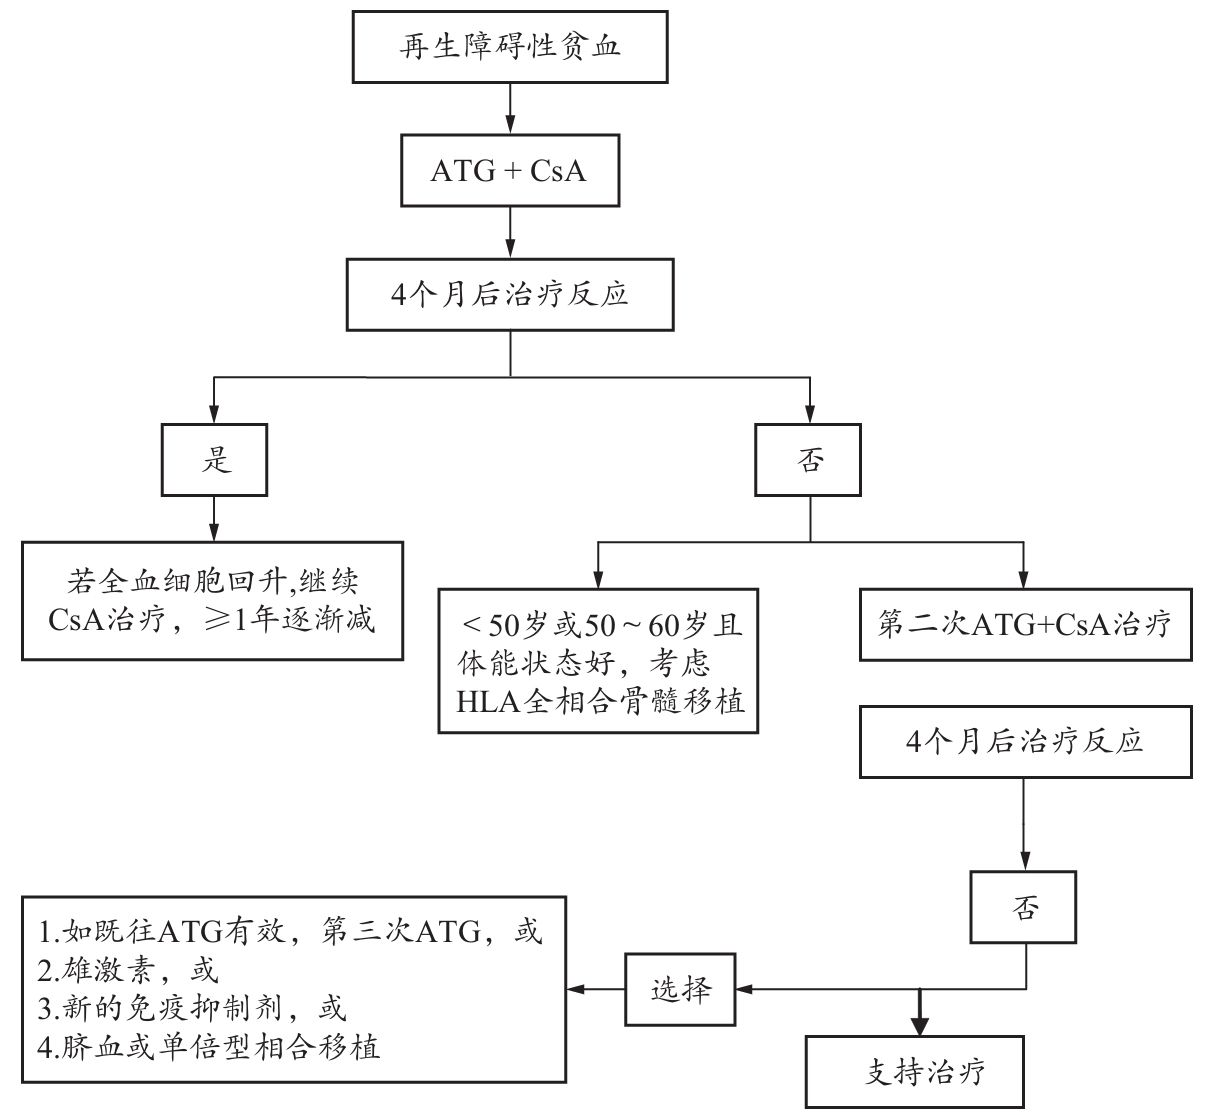
\includegraphics{./images/Image00134.jpg}
 \captionsetup{justification=centering}
 \caption{重型再生障碍性贫血的治疗程序}
 \label{fig5-1-1}
  \end{figure} 

\begin{figure}[!htbp]
 \centering
 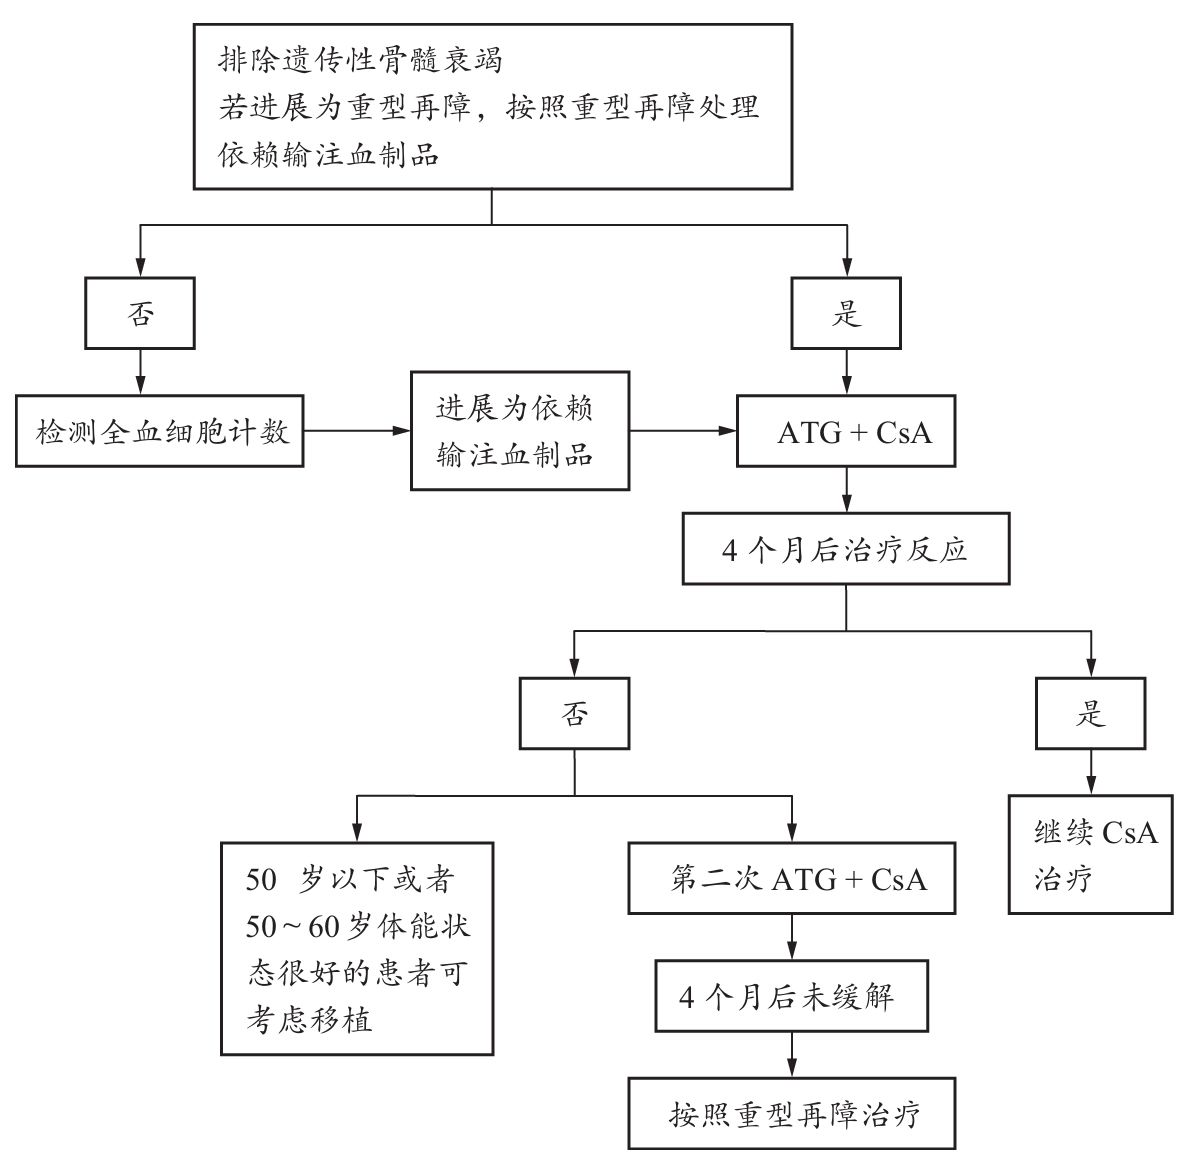
\includegraphics{./images/Image00135.jpg}
 \captionsetup{justification=centering}
 \caption{非重型再生障碍性贫血的治疗}
 \label{fig5-1-2}
  \end{figure} 

【治疗方案】

1. 重型再障的治疗

(1)支持治疗:包括血制品输注、感染的预防和治疗、去铁治疗、心理辅导和一般的支持治疗。

(2)特殊治疗:经确诊的重型再障患者的标准治疗为HLA相合造血干细胞移植,或者抗胸腺球蛋白(ATG)联合环孢素A(CsA)的强化免疫抑制治疗。

兔ATG治疗总量为5mg/(kg·d),静脉滴注第1~5日。由于静脉滴注异种蛋白可能引起严重的过敏反应,在开始大量滴注前必须先进行静脉试验。首先以ATG3mg(法国)或10mg(德国)加入生理盐水100ml,静脉滴注1小时。静脉试验时不用激素,应行心电监护。备好氧气、吸痰器、肾上腺素、地塞米松等抢救药品及器械,并密切观察输液反应。若无反应则开通两个静脉通道:①通道一:ATG5mg/(kg·d)加入生理盐水1000ml,静脉滴注12~16小时滴完。②通道二:先予氢化考的松100mg加入生理盐水500ml,静脉滴注。每日激素用量按泼尼松1mg/(kg·d)计算,每日予氢化考的松100mg,剩余的激素量换算成地塞米松加入5\%葡萄糖500ml静脉滴注,与通道一的时间同步。

猪ATG(武汉生产)治疗总量为30mg/(kg·d),静脉滴注第1~5日。皮试方法:用猪正常免疫球蛋白进行皮试,取0.1ml猪ATG加生理盐水至10ml,稀释至1∶100,于前臂打皮丘,观察15分钟,若有水疱,明显红肿者为阳性。对可疑阳性者,用皮试液滴眼做角膜试验,若出现充血,红肿则为阳性。若皮试阴性,则也采用两通道法用药:①通道一:ATG30mg/(kg·d)加入生理盐水250ml静脉滴注,开始5~10滴/分钟,10分钟后若无不良反应,则逐渐加快速度,2小时内滴完。②通道二:氢化考的松100mg加入5\%葡萄糖500ml静脉滴注,2小时内滴完。

2. 非重型再障的治疗

(1)以雄性激素及中药为主:可予司坦唑醇(康力龙)6~12mg/d,分3次口服;或十一酸睾酮(安特尔)80~160mg/d,分2次口服;或丙酸睾酮100mg,每日1次肌内注射;或达那唑0.2,每日3次口服。也可同时予CsA3~6mg/(kg·d)口服,连续应用3个月以上。

(2)其他刺激造血的药物:再造生血片5片,每日3次口服;或复方皂矾丸7片,每日3次口服;或益血生3片,每日3次口服。

【疗效观察与随访】

1. 观察指标 常见症状、体征、血象与骨髓象。

2. 重型再障疗效标准

(1)完全缓解:Hb正常,ANC\textgreater{}1.5×10$^{9}$
/L,PLT\textgreater{}150×10$^{9}$ /L。

(2)部分缓解:已脱离输注血制品依赖,但未达到完全缓解的指标。

(3)无反应:疾病状态无改善或恶化。

3. 非重型再障疗效标准

(1)完全缓解:Hb正常,ANC\textgreater{}1.5×10$^{9}$
/L,PLT\textgreater{}150×10$^{9}$ /L。

(2)部分缓解:摆脱输注血制品依赖,或至少有一系血细胞较治疗前翻倍或达到正常值,或Hb上升30g/L以上(如最初Hb<60g/L),或ANC上升\textgreater{}0.5×10$^{9}$
/L(如最初ANC<0.5×10$^{9}$ /L),或PLT上升\textgreater{}20×10$^{9}$
/L(如最初PLT<20×10$^{9}$ /L)。

(3)无反应:疾病状态无改善或恶化。

4. 随访 密切观察病情变化,定期复查相关指标。

无论患者接受异基因造血干细胞移植治疗或者ATG联合CsA的强化免疫抑制治疗,均应定期检查血常规和骨髓形态学变化,以评估治疗效果或及时发现疾病复发。对于接受强化免疫抑制治疗者还特别需要随访是否有PNH、MDS、AML克隆的增生,因此在疾病状态发生变化时推荐同时进行骨髓形态学及细胞遗传学检查。2009年英国再障治疗指南还推荐患者每年进行一次PNH克隆的筛查。

【治疗经验与解析】

1.
少数患者可在治疗初期或1~2周时出现速发型超敏反应或血清病。前者典型症状是体温升高、皮肤潮红、水肿、呼吸困难、喘鸣和血压下降。后者常表现为发热、皮疹、肌肉和关节酸痛甚至休克。

ATG的禁忌证:已知对兔蛋白过敏者;血小板严重减少的患者,如少于20×10$^{9}$
/L(因ATG可能引起血小板减少),有增加出血危险;对细菌,病毒感染尚未得到治疗控制者;妊娠或哺乳期妇女。

2.
使用中应将ATG药品的批号保留在病历中,每天使用时应核对批号。同一次治疗的批号必须相同。为预防过敏性休克,急救治疗设备必须准备妥当,并有专人监护尤其是第1日用药。每天的药物必须在12~16小时内滴完(22~24滴/分钟)。ATG不能与葡萄糖、肝素钠、血液、血源性制品和含脂类溶液混合使用。

3.
雄激素治疗后的长期生存者发展为克隆性血液病的可能性基本上与用免疫抑制剂治疗的患者相同。雄激素使用中严密检测不良反应,特别应注意肝脏毒性(康力龙最常见),应定期监测肝功能和给予保肝药物。对于处于生长发育期的儿童和青少年需慎用。

4.
泼尼松可促进血红蛋白增长,控制溶血,但其效果不肯定,且可能导致股骨头坏死,现已少用。英国2009年再障治疗指南中明确指出糖皮质激素对再障的疗效不确切,而且增加了细菌、真菌感染的风险,并增加消化道溃疡的发生率,不推荐使用。

5.
目前中药主要用于非重型再障的治疗,所开发的许多成药已在临床广泛应用。当患者以出血发热为突出症状时,中医认为肾阴虚,治疗以滋补肾阴为主。当患者的发热、出血被控制,以贫血为主要症状时,中医认为属肾阳虚,治疗以补肾阳为主。而由肾阴虚转为肾阳虚的过程中常有一个肾阴阳两虚的阶段,治疗以阴阳双补。当患者大便溏稀时诊断为脾肾两虚可加用健脾药。

6. CsA的应用

(1)常用剂量为3~6mg/(kg·d),每个个体所需的剂量有需要的按血药浓度尝试调整,初始治疗时通常维持全血谷浓度200ng~400ng/ml。疗程不少于0.5年,多数需1~2年,待血象正常或平稳后才考虑逐渐减量。用药时需定期监测血压、肝肾功能、电解质等指标。复发者仍按初始剂量给药。

(2)不良反应有高血压、牙龈及毛发增生、皮肤色素沉着、肝功能损害、氮质血症、增加感染危险等。用药期间需定期检查肝、肾功能,有血清肌酐水平增高是降低用药量的指征,以免出现不可逆的慢性肾病(以间质纤维化、小管萎缩为特征)。CsA与雌激素、雄激素、西咪替丁、地尔硫@、红霉素、酮康唑、伊曲康唑、伏立康唑等合用,可增加本品的血浆浓度。故与上述各药合用时须慎重。用CsA时如输注贮存超过10日的库存血或与保钾利尿剂、含高钾的药物等合用,可使血钾增高。

(3)患者如有下列指标之一,提示对CsA有较好反应:①骨髓粒红比值\textgreater{}0.6。②CsA能促进患者粒单细胞集落刺激单位体外生长。③HLA-DR2位点阳性。④骨髓单个核细胞干扰素-γmRNA阳性等。

7.
造血细胞生长因子曾经广泛的被应用于重型再障的治疗。但是新的指南指出促红细胞生成素(EPO)治疗再障是无效的,因为再障患者本身血清EPO水平就是显著增高的,而EPO使用可能产生抗EPO抗体而引起贫血恶化,与CsA联合应用可能加重毒性(高血压)。

促进血小板生成剂如IL-11及促血小板生成素(TPO)的疗效也不确定。

粒细胞集落刺激因子(G-CSF)用于粒缺的治疗,常见的副作用有发热、头痛、肌肉痛、关节痛等,一般多能耐受。但是对于其治疗再障的疗效尚无有说服力的证据,循证医学提示短程的皮下注射G-CSF5μg/(kg·d)并无增加患者抗细菌和真菌的能力。G-CSF治疗后有反应者一般是仍有残留的部分粒细胞造血活性患者。因此推荐在使用G-CSF无效后即停止此药。

8.
来自同胞的HLA全相合的Allo-HSCT移植有希望治愈本病,无关供者HLA全相合的Allo-HSCT移植治疗效果近年来有明显提高,在特定情况下也可以考虑。而免疫抑制治疗尚不能使血细胞计数完全恢复正常,存在复发的危险。本病经Allo-HSCT后最初3个月病死率最高,多死于移植物排斥(发生率5\%~70\%)或移植物抗宿主病(发生率约为80\%)。关于移植物的选择,目前认为骨髓的治疗效果要优于动员的外周血干细胞。适用于<40岁的重型再障患者;移植前应减少输血,输血<20次者效果好;女性供者以妊娠前、未输血者效好;同性间移植或男性供者效果好。非清髓HSCT因副作用较小,近年来亦用于治疗再障。

\subsection{阵发性睡眠性血红蛋白尿症}

阵发性睡眠性血红蛋白尿症(PNH)是红细胞膜的获得性缺陷引起的对激活补体异常敏感的一种慢性血管内溶血。临床表现以与睡眠有关的、间歇发作的血红蛋白尿为特征,可伴有全血细胞减少或反复血栓形成。

PNH是一种原因不明的克隆性疾病。患者体内正常造血干细胞与异常克隆并存。目前认为患者的骨髓因受到某种有害因素的损伤,而引起造血细胞的基因突变,产生病理性克隆,这种异常细胞达到一定数量后,则可发病。PNH的红细胞有许多异常,其中最重要的是对补体溶血的敏感度显著提高。

【治疗方案】 尚无特殊疗法,以支持和对症治疗为主。对于有轻度贫血、血红蛋白尿轻的患者应尽量减少用药。应避免诱发因素,减少溶血的发生,积极防治感染,避免过度劳累和精神紧张。对于有严重贫血伴有溶血危象、血栓形成、感染的患者应及时治疗。

1.
支持治疗 对于严重贫血患者需酌情输注洗涤红细胞改善症状。大多数反复发作的PNH患者会逐渐出现铁缺乏,可适当补充铁剂。另外可适当补充叶酸。

2.
控制溶血发作 在溶血发作期可口服小苏打或静脉滴注5\%碳酸氢钠碱化利尿。目前控制PNH溶血的主要药物是肾上腺皮质激素。泼尼松、地塞米松、氢化可的松为常用制剂。开始时可用泼尼松40~60mg/d,发作停止后逐渐减量维持。右旋糖酐在体内有抑制溶血的作用,输入6\%右旋糖酐500~1000ml可以阻止血红蛋白尿的发作。适用于伴有感染、外伤、输血反应和腹痛危象者,但长期应用可能发生出血并发症。抗氧化药物对细胞膜有保护作用,常用维生素E,每日300mg,分3次口服,但效果并不肯定。

3. 其他治疗

(1)雄激素:能够刺激造血、提高血红蛋白水平。口服康力龙6~12mg/d或羟甲烯龙10~50mg/d或达那唑400~600mg/d。约有50\%骨髓低增生的PNH患者对雄激素有反应。但鉴于雄激素的不良反应,在治疗后6~8周无明显疗效应停用。

(2)化疗药物:PNH是一种不均质的造血干细胞克隆性疾病,而正常克隆较PNH克隆耐受,恢复快的优势,通过反复化疗,使正常克隆逐步替代PNH克隆。但多数以后会复发。常用的方案为COAP和MP方案,有效率60\%左右,但因PNH对化疗敏感,会发生严重的骨髓抑制,故需加强支持治疗。

(3)免疫抑制剂:抗胸腺细胞球蛋白(ATG)、环孢素A等,联合粒细胞刺激因子对部分患者有效,但不能改变PNH克隆的大小。

(4)单克隆抗体(依库珠单抗):可直接作用于补体C5上,阻断其作用,使溶血减少,达到减少输血依赖并提高生活质量的目的。用法:每周输注600mg共4周,之后1周输注900mg,然后每2周输注900mg共12周结束。后续治疗剂量的频率从每14日900mg增加到每12日900mg,以保证在12个月的治疗间期完全阻断补体。

(5)造血干细胞移植:理论上异基因造血干细胞移植可根治异常造血干细胞病,但本病为良性疾病,有10\%~15\%可以在病后10~20年自然缓解。严重PNH反复常规治疗无效或严重贫血伴有骨髓增生不良的病例建议造血干细胞移植。

4. 并发症的防治

(1)感染:是诱发急性溶血的诱因,也是我国PNH的主要死亡原因。预防和控制至关重要。

(2)血栓形成:口服华法林抗凝剂有防止血栓的作用,但有出血的危险,应慎重。

(3)合并症:PNH还可并发胆石症和肾衰竭等,予以相应的预防和治疗。

【疗效观察与随访】

1.
观察指标 常见症状、体征、血常规、骨髓常规、出凝血指标、尿常规等。患者观察病情的重要指标是尿色,尤其是晨尿,出现浓茶色尿或者酱油色尿提示病情发作,也有些患者首先出现乏力、胸腰腹疼痛、发热等症状而尿色变化不明显。

2. 疗效评估 好转标准:症状减轻,溶血改善,感染控制。

3.
随访 密切观察病情变化,定期复查血常规,流式细胞术检测CD55/CD59阴性克隆的数量及骨髓形态学检查。

【治疗经验与解析】

1. 如同时有血管栓塞可口服华法林,但注意过量有出血危险。

2.
对于血红蛋白尿丢失铁而伴有缺铁的患者,铁剂治疗有助于改善贫血。铁剂可使活性氧产生,PNH细胞对氧化损伤很敏感,易诱发血红蛋白尿。但补铁后红细胞生成增加,对补体敏感的红细胞增多,会加重或诱发溶血,所以缺铁者可应用小剂量的铁治疗(常规量的0.1~0.3),如有溶血,则停用。

3.
低分子右旋糖酐具有抑制PNH细胞溶血的作用,长期应用可发生出血并发症,对心功能不全应注意不可过量和长期应用。

4.
即使是输注洗涤红细胞也有可能再诱发溶血,因此除非贫血很重或高龄、高热、心功能欠佳的患者,应尽量减少输红细胞悬液。

5.
PNH在临床上有时与再生障碍性贫血难以区分。10\%~20\%的再生障碍性贫血患者会在病程中出现PNH的表现。另外有些PNH的患者也会在病程中出现骨髓衰竭表现。对于这些现象在患者诊疗过程中需要注意。

\subsection{骨髓增殖性肿瘤}

骨髓增殖性肿瘤(MPNs),既往称为骨髓增殖性疾病(MPDs),是一类以一系或多系髓系细胞(包括红系、粒系和巨核系)增殖为主要特征的克隆性造血干细胞疾病。主要包括慢性髓性白血病(CML)、真性红细胞增多症(PV)、原发性血小板增多症(ET)和原发性骨髓纤维化(PMF)四种经典类型,另外还包括慢性中性粒细胞白血病(CNL)、慢性嗜酸粒细胞白血病(CEL)、高嗜酸粒细胞综合征(HES)、肥大细胞增生症以及不能分类的MPN。本章重点介绍经典的MPN疾病(CML、PV、ET及PMF)的治疗指南。

{(一)慢性髓性白血病}
 慢性髓性白血病是一种克隆性造血干细胞疾病,主要表现为骨髓和外周血中持续性白细胞数目异常增高,以中幼粒细胞及以下阶段为主。染色体9号与22号相互易位形成Ph染色体,并产生BCR-ABL融合基因,翻译的BCR-ABL融合蛋白是该病重要的分子标志。该蛋白具有异常的酪氨酸蛋白激酶(PTK)活性,能通过作用于Ras相关的信号传递分子及上调Bcl-X{L}
抗凋亡基因活性等途径促进细胞增殖、抑制凋亡,导致CML的发生。CML病程发生较慢,临床症状轻微,可有明显脾大,甚至巨脾,周围血的中性粒细胞显著增多。

慢性髓性白血病占白血病的15\%~25\%,各种年龄均可发病,以中年最多见,男性略多于女性。可分为三期,慢性期(稳定期),加速期(活动期)和急变期。起病缓慢,早期常无自觉症状。大多数患者因急变而死亡。

【治疗程序】

1. CML初始治疗程序 如图\ref{fig5-1-3}所示。

\begin{figure}[!htbp]
 \centering
 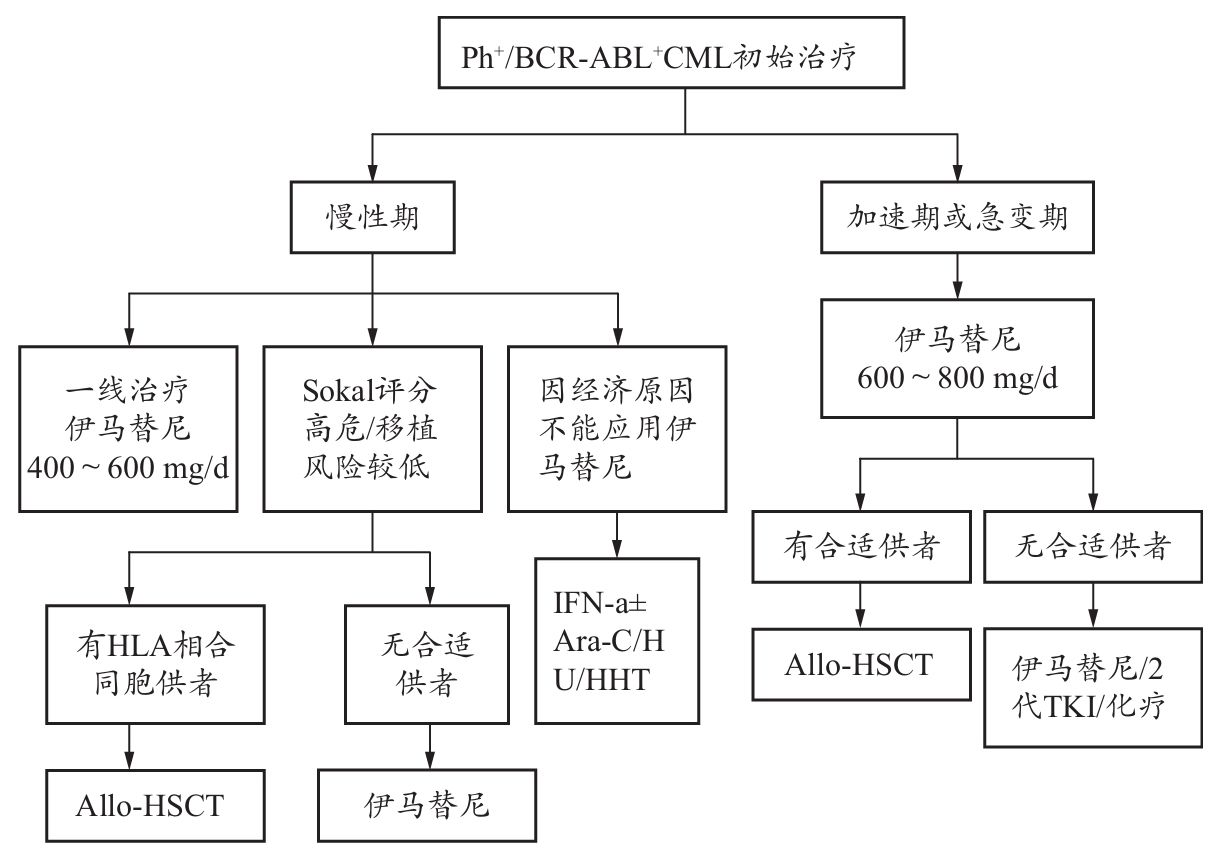
\includegraphics{./images/Image00136.jpg}
 \captionsetup{justification=centering}
 \caption{慢性髓性白血病的初始治疗程序}
 \label{fig5-1-3}
  \end{figure} 

2. 初始治疗后,根据疗效调整治疗方案 如图\ref{fig5-1-4}所示。

\begin{figure}[!htbp]
 \centering
 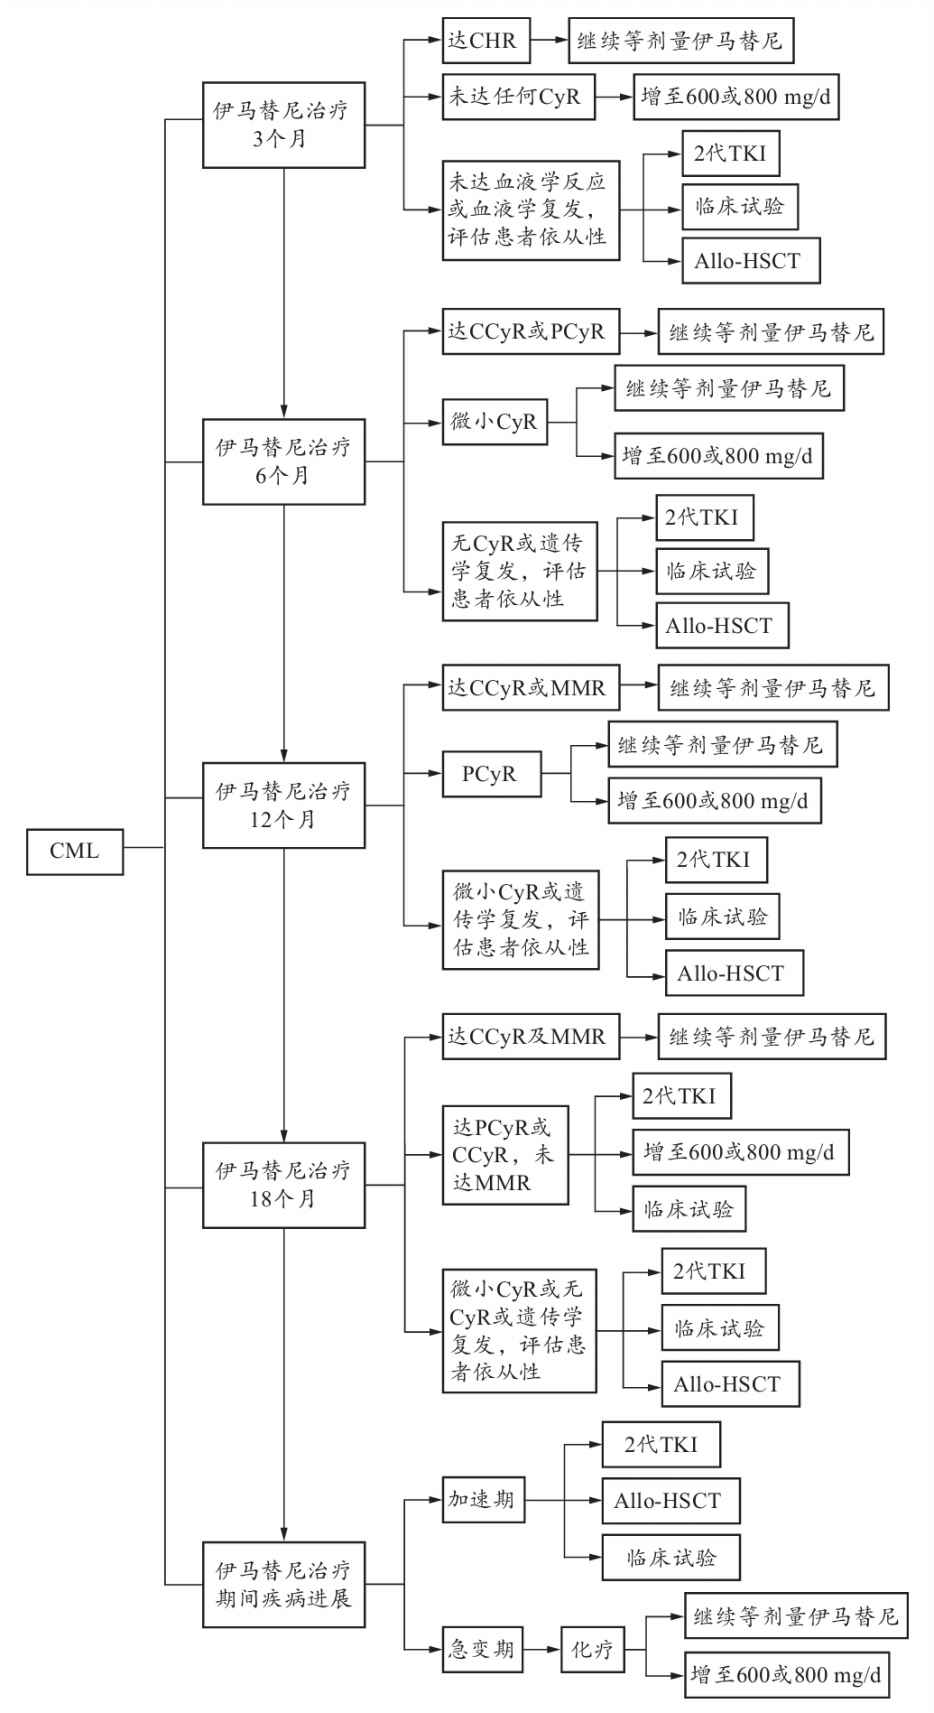
\includegraphics{./images/Image00137.jpg}
 \captionsetup{justification=centering}
 \caption{慢性髓性白血病根据初始治疗的疗效调整治疗方案}
 \label{fig5-1-4}
  \end{figure} 

3. 以IFN-α为基础的治疗及方案调整 如图\ref{fig5-1-5}所示。

\begin{figure}[!htbp]
 \centering
 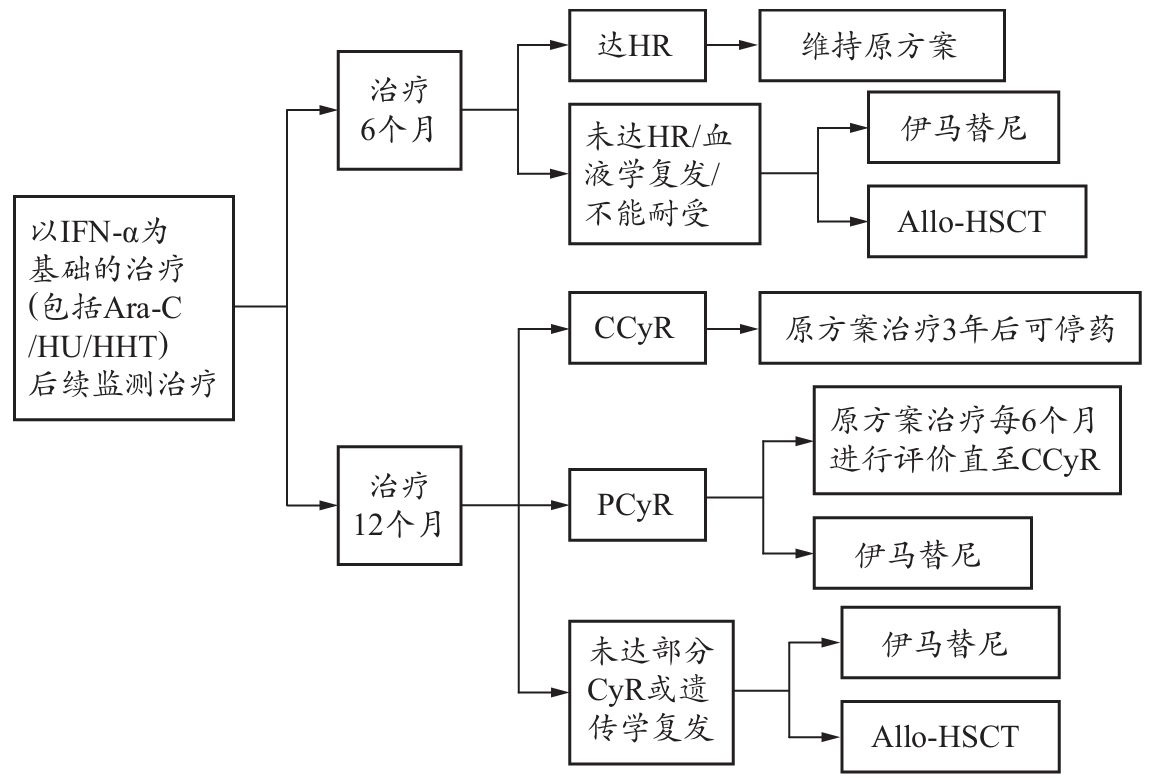
\includegraphics{./images/Image00138.jpg}
 \captionsetup{justification=centering}
 \caption{以IFN-α为基础的治疗及方案调整}
 \label{fig5-1-5}
  \end{figure} 

4. Allo-HSCT后续治疗 如图\ref{fig5-1-6}所示。

\begin{figure}[!htbp]
 \centering
 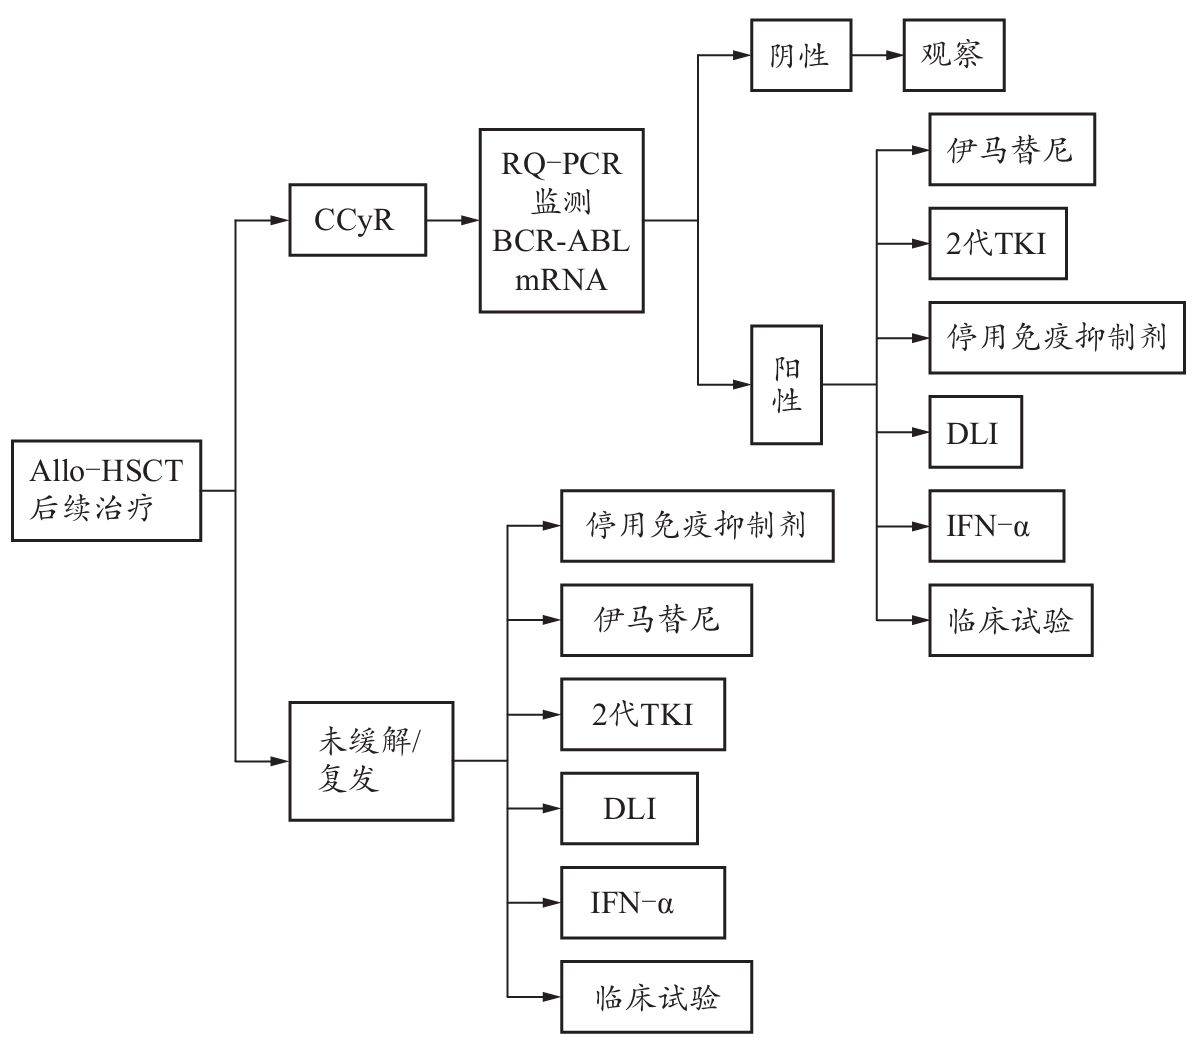
\includegraphics{./images/Image00139.jpg}
 \captionsetup{justification=centering}
 \caption{Allo-HSCT后续治疗}
 \label{fig5-1-6}
  \end{figure} 

【治疗方案】

1. 一般治疗

(1)化疗:虽可使大多数CML患者达到血液学部分或完全缓解,但患者的中位生存期(40个月左右),与不治疗相比并未得到明显改善。

1)羟基脲:起效快,但持续时间较短。用药后2~3日白细胞就迅速下降,停药后又很快回升。初始剂量为1~3g/d,分2次口服,待白细胞减至20×10$^{9}$
/L左右,剂量减半。降至10×10$^{9}$
/L时,改为小剂量(0.5~1g/d)维持治疗。

2)干扰素α:剂量为(3~9)×10$^{6}$
U/d,皮下或肌内注射,每周3~7次。持续用数月至2年不等。因对胎儿发育影响较小,对于妊娠期妇女可以作为一线治疗。约70\%患者获得血液学缓解,30\%患者获得细胞遗传学缓解,对加速和急变期患者无效。该药与小剂量阿糖胞苷联合用,可提高疗效。

3)白消安:属烷化剂,能选择性抑制较成熟的幼粒细胞,初始剂量为4~6mg/d,口服。用药2~3周,外周血白细胞开始减少,故应掌握剂量。当WBC降至20×10$^{9}$
/L时宜暂停药,因停药后白细胞减少可持续2~4周。待稳定后改小剂量(每1~3日2mg),使WBC保持在(7~10)×10$^{9}$
/L。目前临床应用较少。

4)其他:包括靛玉红,小剂量Ara-C,三溴甘露醇、6-MP、苯丁酸氮芥、环磷酰胺及其他联合化疗等。

化疗时宜加用别嘌醇(100mg,每日3次),并保持每日尿量在1500ml以上和碱化尿液,防止尿酸性肾病。待白细胞下降后停药。

(2)造血干细胞移植:Allo-HSCT是目前唯一能治愈CML的方法。疗效与病期相关,慢性期疗效最好;复发率随病期进展而增加。移植相关死亡和疾病复发是移植的主要风险。移植前评估可帮助治疗选择,欧洲血液和骨髓移植组(EBMT)根据患者年龄、疾病分期、病史长短、供受者性别、HLA相合供者来源5个变量进行移植前风险评估,对积分≥3者,建议先接受伊马替尼治疗,或接受非清髓移植以规避风险。研究表明,0~2分者3年总生存率70\%,3~4分者为50\%,≥5分者为30\%,对于高危患者也可采用HLA不全相合的Allo-HSCT。对移植后复发患者可行供者淋巴细胞输注(DLI)、伊马替尼、第2代TKI、IFN-α治疗或临床试验。

(3)白细胞单采:采用血细胞分离机可除去大量白细胞,减少体内白细胞数量。主要用于白细胞淤滞症,以缓解危险状况。也可用于急需治疗的孕妇。

(4)脾放射和脾切除:目前脾区放射偶用于伴有胀痛的巨脾以缓解症状,目前多已弃用。

2.
分子靶向治疗 甲磺酸伊马替尼(Glivec,IM,格列卫)能与BCR-ABL酪氨酸激酶作用,进而抑制白血病细胞的增殖并诱导这些细胞的程序性死亡。慢性期、加速期及急变期均可作为一线用药。常用剂量为400mg/d,可逐步增量至600mg/d,最大可达到800mg/d。不良反应主要为恶心、局限性水肿,肌肉痛性痉挛、腹泻、呕吐、皮疹、乏力及血细胞减少。初治CML-CP,IM治疗1年后CHR、MCR和CCR分别为96\%、85\%和69\%,随治疗时间延长疗效增高,5年CCR
87\%,总生存率90\%。

第2代酪氨酸激酶抑制剂:达沙替尼为SRC和ABL激酶双重抑制剂,尼洛替尼为ABL激酶抑制剂,均为第2代TKI的代表,可以逆转伊马替尼耐药,用于治疗伊马替尼耐药或不能耐受的CML患者。

【疗效观察与随访】

1. 观察指标 常见症状和体征,白细胞、骨髓象等。

2.
疗效评估 由于CML有明确和独特的遗传学和分子标志,可依此来进行治疗反应评估。在进行评估时,应包括血液学、骨髓细胞遗传学及分子学结果(表\ref{tab5-1-1})。

\begin{longtable}[]{@{}lp{4cm}p{4cm}p{4cm}@{}}
    \caption{CML治疗反应定义及监测}
    \label{tab5-1-1}\\
\toprule
& 血液学反应(HR) & 细胞遗传学反应(CyR) &
分子学反应(MoR)\tabularnewline
\midrule
\endfirsthead
\caption[]{CML治疗反应定义及监测}\\
\toprule
& 血液学反应(HR) & 细胞遗传学反应(CyR) &
分子学反应(MoR)\tabularnewline
\midrule
\endhead
\bottomrule
\endfoot
定义 & CHR WBC<10×10$^{9}$ /L,PLT<450×10$^{9}$
/L,外周血无幼稚髓细胞,骨髓原始细胞<5\%,无疾病的症状、体征,可触及的脾肿大消失
& CCyR Ph{+} 0;PCyR Ph{+}
1\%~34\%;mCyR Ph{+}
35\%~90\%;noCyR Ph{+} \textgreater{}90\%
& CMoR BCR-ABL转录本阴性;MMoR
BCR-ABL转录本较治疗前基数下降≥3log\tabularnewline
监测频率 & 每周1次直至CHR,随后每3个月1次 &
每3个月1次直至CCyR,随后每3~6个月1次 &
每3个月1次,疗效欠佳或治疗失败时测定BCR-ABL区点突变\tabularnewline
监测方法 & 全血细胞计数+外周血分类 &
骨髓细胞遗传学分析荧光原位杂交(FISH) &
定量聚合酶链反应(QPCR)\tabularnewline
\end{longtable}

注:WBC=白细胞计数;PLT=血小板计数;CHR=完全血液学反应;CCyR=完全细胞遗传学反应;PCyR=部分细胞遗传学反应;mCyR=微小细胞遗传学反应;noCyR=无细胞遗传学反应;CMoR=完全分子学反应;MMoR=主要分子学反应

3. 随访 密切观察病情变化,定期复查相关指标,指导病后保健。

【治疗经验与解析】

1.
关于高白细胞治疗,应先以降低白细胞、减少相关并发症为治疗目的。可首选羟基脲,白细胞过高时可采用白细胞分离术以防白细胞淤滞症。

2.
伊马替尼耐药的处理,主要策略包括:在排除服药不规范,患者依从性差等因素后,需要进行ABL激酶区突变基因的筛查。根据TKI基因变化类型来选择提高TKI剂量、改用2代TKI药物,或是进行HSCT。

3.
伊马替尼应用过程中的疾病监测对指导治疗、判断预后十分重要,如监测HR、CyR及MR。

4.
伊马替尼可使大部分患者获得CyR甚至MR,延长生存期并提高生活质量;Allo-HSCT是目前唯一能够根治CML的手段,但受到患者年龄和供者条件等因素的限制,并且移植风险也较大。所以,应根据患者的病情和年龄、有无合适的移植供者、经济条件和所在医院的医疗水平等因素,选择伊马替尼、Allo-HSCT、IFN-α或化疗,进行个体化治疗。Sokal评分高危而移植风险较低的CML慢性期患者,如果有HLA相合同胞供者,可以选择一线Allo-HSCT;对于HLA不相合者不推荐Allo-HSCT,但因经济原因或者患者移植意愿强烈者可考虑移植。

{(二)真性红细胞增多症}
 真性红细胞增多症(PV)简称真红,是一种克隆性的以红细胞异常增殖为主的慢性MPNs。其外周血总容量绝对增多,血液粘滞度增高,常伴有白细胞和血小板升高,脾大,病程中可出现出血、血栓形成等并发症。发病高峰年龄集中在50~60岁,因此是一种中老年性疾病。男性稍多于女性,临床特征有皮肤粘膜红紫、肝脾大及血管性与神经性症状,起病隐袭,病程进展缓慢。

【治疗方案】 治疗目的是尽快使血容量及红细胞容量接近正常,抑制骨髓造血功能,从而缓解病情,减少并发症。治疗必须根据年龄、性别、身体状况、临床表现以及血液病学检查结果予以个别处理。

1. 经典治疗

(1)对症支持治疗:有高尿酸血症者,可用别嘌醇,如合并痛风性关节炎,可并用秋水仙碱、糖皮质激素。皮肤瘙痒顽固者可以试用抗组胺类药物,如息斯敏、西咪替丁。对于有静脉血栓并发症的患者,不主张使用血小板抑制剂,如阿司匹林、双嘧达莫,因其并不能减少血栓形成,反而增多胃肠道出血机会。

(2)静脉放血及红细胞单采术:静脉放血可在较短时间内使血容量降至正常,症状减轻。每隔2~3日放血200~400ml,直至Hct<0.45。采用血细胞分离机进行治疗性红细胞单采术,可迅速降低血细胞比容和血液粘度,改善临床症状,适用于伴白细胞或血小板减少或妊娠的患者。

(3)骨髓抑制治疗:

1)羟基脲:对PV有良好抑制作用,其致白血病的长期安全性研究仍在进行中。患者先放血使Hct恢复正常40\%~45\%后给予羟基脲口服。每日剂量为15~20mg/kg。如白细胞维持在3.5~5.0×10$^{9}$
/L,可长期间歇应用。

2)烷化剂:通过抑制骨髓增殖起作用,有效率80\%~85\%。常用的有白消安、环磷酰胺、左旋苯丁酸氮芥(瘤可然)及马法兰(美法仑、苯丙氨酸氮芥)。开始剂量:环磷酰胺为100~150mg/d;白消安、美法仑及苯丁酸氮芥为4~6mg/d。缓解后停用4周后可给维持量,环磷酰胺为每日50mg,白消安为每日或隔日2mg。

3)高三尖杉酯碱:常用剂量2~4mg/d肌内注射或加入5\%葡萄糖溶液中静脉滴注,7~14日为1个疗程。通常1个疗程疗效可持续3~6个月,复发后再用仍有效。

4)放射性核素治疗:{32}
P的β射线损伤DNA和RNA,从而抑制血细胞生成,使细胞数降低,达到治疗效果。有效率为80\%~90\%。

5)干扰素α:抑制PV克隆的增殖,可用于不能耐受羟基脲或药物不能控制外周血象的患者,标准的开始剂量为3.0×10$^{6}$
U皮下注射,每周3次。治疗3个月后脾脏缩小,缓解率可达80\%。但有效性和长期使用的安全性仍在进一步研究和观察中。

2.
新型治疗 JAK2V617F点突变抑制剂:各国研究机构及制药公司正在加紧开发,但其应用于临床尚有待时日。

【疗效观察与随访】

1. 观察指标 常见症状、体征、血象、骨髓象、脾B超检查等。

2. 疗效评估

(1)完全缓解:临床症状消失,皮肤、粘膜从红紫恢复到正常,原肿大的肝脾显著回缩至不能触及,血红蛋白、白细胞和血小板计数降至正常。若红细胞容量也恢复正常,则称完全缓解。

(2)临床缓解:临床及血象恢复如上,但红细胞容量尚未恢复正常或仍可触及脾脏。

(3)好转:临床症状明显改善,皮肤、粘膜红紫有所减轻,原增大的肝脾有所回缩,血红蛋白下降30g/L以上。

(4)无效:临床症状、体征,以及血象无变化或改善不明显。

3.
随访 注意病情观察,观察临床症状、体征变化,注意肝脾大及恢复情况。监测血常规,注意白细胞、血小板及血红蛋白的变化。

【治疗经验与解析】

1.
年轻患者如无血栓并发症可单独采用放血疗法,但放血后有引起红细胞及血小板反跳性增高的可能,注意反复放血有加重缺铁的倾向。老年及有心血管疾病患者,因放血可能引发栓塞并发症,应慎用,每次不宜超过200~300ml,间隔期可稍延长。

2. 放射性核素{32}
P有增加急性白血病的转化的风险,因此要慎用(最好避免用于70岁以下的患者)。

3.
若化疗应常规予碱化尿液、抑制尿酸合成、嘱患者大量饮水等支持治疗。烷化剂有引起白血病的风险,应警惕。

{(三)原发性骨髓纤维化}
 原发性骨髓纤维化(PMF)为造血干细胞异常所致的慢性MPNs。病理上示骨髓弥漫性纤维组织增生,常伴有髓外造血(或称髓外化生),主要在脾,其次在肝、淋巴结等。各系造血细胞不同程度过度增生或增生减低,外周血出现畸形红细胞及幼粒、幼红细胞性,脾显著增大,不同程度的骨质硬化,骨髓常干抽。可与其他类型MPNs相互转化,晚期骨髓衰竭,少数转化为急性白血病。

【治疗程序】 如图\ref{fig5-1-7}所示。

\begin{figure}[!htbp]
 \centering
 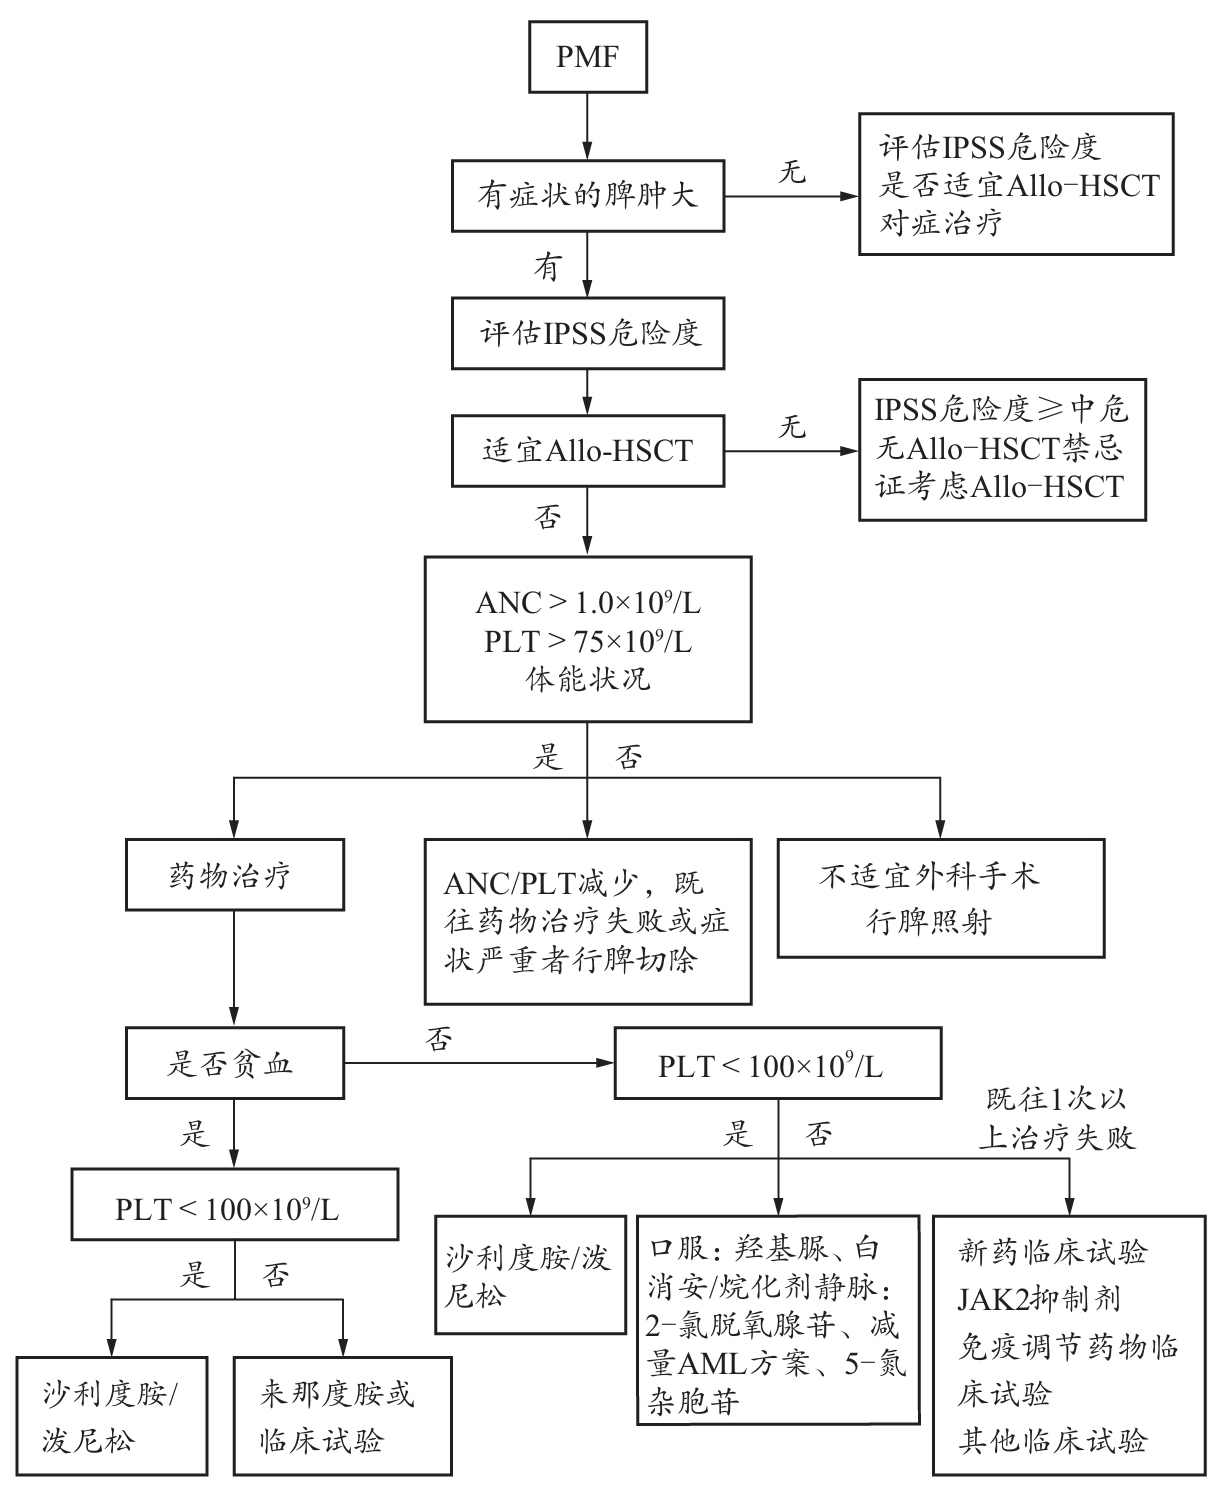
\includegraphics{./images/Image00140.jpg}
 \captionsetup{justification=centering}
 \caption{原发性骨髓纤维化的治疗程序}
 \label{fig5-1-7}
  \end{figure} 

【治疗方案】 PMF患者自初诊后,中位生存期约为5年左右。危险因素有:①Hb<100g/L;②年龄\textgreater{}64岁;③高分解代谢症状(体重减低,疲倦,盗汗,低热);④WBC增加(\textgreater{}30×10$^{9}$
/L)或减少(<4×10$^{9}$
/L);⑤外周血原始细胞≥1\%;⑥细胞遗传学异常(+8,12p-)。根据以上因素,将患者的预后分为三类:低危(无危险因素)、高危(具有2个或2个以上危险因素)、中危(介于低危和高危之间)。低危患者平均寿命可达10年,高危者为3年。因此,低危者不需立即治疗。除造血干细胞移植有治愈PMF的可能外,大部分治疗的目的仍是减轻症状和改善造血功能,阻止纤维化病变的进展。

1. 经典治疗

(1)纠正贫血:红细胞生成素水平低者可用人重组EPO,雄激素具有改善贫血症状的作用,有效率30\%~40\%。严重贫血可输红细胞,要求血细胞比容保持在0.25以上。

(2)化学治疗:适用于白细胞和血小板明显增多、有显著脾大而骨髓造血障碍不很明显时。首选羟基脲治疗,剂量通常为0.5~1.0/d,每周2~3次口服。具体的剂量需考虑治疗前血细胞计数。治疗过程中需要密切观察血象。

(3)干扰素:干扰素α和γ可以抑制巨核祖细胞及骨髓成纤维细胞的生长,剂量为300万~500万U/次,皮下注射,每周3次。

(4)减轻脾肿大:

1)脾切除适应证包括:①持续严重的体重下降、疲倦、低热、盗汗等症状;②持续明显的脾区疼痛(包括脾梗死引起的顽固疼痛);③并发腹水或静脉曲张出血的门脉高压;④药物难治的依赖输血的贫血。脾切除手术并不影响MF患者的长期生存率。

2)脾照射治疗适应证包括:巨脾引起腹部及全身相关症状,存在脾切除手术禁忌证如不适于麻醉、弥散性血管内凝血、血细胞少或门脉高压或拒绝脾切的患者。照射剂量必须个体化,照射期间要监测血象、疗效、毒副作用,及时调整剂量。

(5)维生素D{3}
:有抑制巨核细胞增殖,并诱导髓细胞向单核及巨噬细胞转化作用,并有逆转骨髓纤维化的可能。

(6)造血干细胞移植:对于年轻患者(<45岁)可以考虑HLA全相合的异基因造血干细胞移植(5年生存率62\%)。但对于\textgreater{}45岁以上的患者移植后疗效很差(5年生存率14\%),故需要慎重。

2.
新型治疗 有研究者发现98\%的PMF患者存在血管生成进行性增加,并造成病情加重。近年来对沙利度胺(反应停)治疗PMF的研究取得了很大进展。单药治疗约有20\%的患者贫血改善,25\%~80\%的血小板有反应,但对于脾肿大作用甚微。可采用递增的方法单独服用沙利度胺治疗,每日100~800mg。亦可采用小剂量反应停泼尼松联合治疗PMF,前三个月每日服用沙利度胺50mg,同时口服泼尼松,第1个月0.5mg/(kg·d),第2个月0.25mg/(kg·d),第3个月0.125mg/(kg·d)。患者耐受性好,不良反应小,疗效较通常剂量明显提高,血液学改善明显。

【疗效观察与随访】

1. 观察指标 常见症状与体征,血常规、骨髓常规,肝、脾B超检查等。

2. 疗效评估

(1)好转:临床无症状,脾缩小达1/2或以上,血细胞数达正常范围,无幼稚粒、幼稚红细胞,骨髓增生程度正常。

(2)进步:临床症状有明显改善;脾较治疗前缩小,但未达1/2;血细胞数至少一项达正常范围,幼稚粒、幼稚红细胞较治疗前减少1/2或以上。

(3)无效:未达进步标准者。

3.
随访 注意观察临床症状、体征变化,特别是肝脾肿大情况。监测血常规,注意复查骨髓形态学及病理活检检查,及时判断是否发生疾病的转变。

【治疗经验与解析】

1. 化疗虽可缩小脾脏,提高血红蛋白,但同时亦常可引起骨髓抑制,需加注意。

2.
由于50\%患者具有JAK2V617F突变,JAK2靶向抑制剂则显示出美好的治疗应用前景。如INCB018424可选择性抑制JAK1和JAK2途径,显著缩小患者脾脏大小,从而改善临床症状。另外,增加INCB018424剂量还可观察到炎症因子释放的减少及症状的改善。其他类似的处于研发阶段的药物还有IG101348、XL019等,初步研究显示都可缩小脾脏。但到目前为止,没有一种JAK2抑制剂可显著改善血细胞减少、纤维化和骨髓的组织学改变,有待进一步研究。

3.
本病常见的死因为严重的贫血、感染、心功能不全和出血等,约20\%患者最后可转化为急性髓系白血病。

{(四)原发性血小板增多症}
 原发性血小板增多症(ET),亦称特发性血小板增多症、出血性血小板增多症,为多能干细胞克隆性疾病。其特征是血小板水平显著持续性增多而功能异常,骨髓中巨核细胞过度增殖,伴有出血及血栓形成,脾常肿大。本病较少见,好发于中老年人,女性略多于男性。

【治疗方案】 治疗目的是减少血小板以控制和预防出血、血栓形成和栓塞。

1. 经典治疗

(1)骨髓抑制剂:首选羟基脲,也可应用白消安或环磷酰胺等。血小板\textgreater{}1000×10$^{9}$
/L者,可用白消安4~8mg/d、环磷酰胺100~200mg/d、羟基脲15mg/(kg·d)等,可重复使用。

(2)放射性核素:{32}
P为治疗本病的重要手段。效果佳,见效快。可口服或静脉注射,首次剂量为(11.1~14.8)×10$^{7}$
Bq,必要时3个月后重复给药。

(3)干扰素α:对人巨核细胞前体细胞有抗增殖作用,故对本病亦有效。但停药后易复发。剂量为300万~500万U/次,皮下注射,每周3次。

(4)血小板单采术:可迅速减少血小板量,改善状态。在紧急情况下(手术前、伴急性胃肠道出血的老年患者、分娩前及骨髓抑制药不能奏效时)采用。

(5)出血和血栓、栓塞的治疗:出血以继发于血栓形成者较多。可选用抗血小板粘附和聚集的药物(如双嘧达莫、阿司匹林)能改善出血倾向。如发生血栓形成或栓塞,可用纤溶激活剂治疗。

2. 新型治疗

(1)危险度分层治疗:近年来随着大规模的临床研究,危险度分层治疗的方案也在逐步完善(表\ref{tab5-1-2})。在低危组患者中,血栓栓塞发生率很低,细胞毒药物治疗无益于患者,绝大多数学者不主张使用。尽管低剂量的阿司匹林治疗可缓解血管运动性症状,但是它是否能够预防低危组患者的血栓形成尚未有定论。对于中危组的患者是否适用于细胞毒药物治疗是有争议的。一般来讲,中危组的育龄女性和孕妇禁用细胞毒药物治疗,可以应用干扰素α治疗;而对于其他血小板数量大于1500×10$^{9}$
/L的中危组患者,细胞毒药物的治疗可以降低血栓和出血发生率。对高危组ET患者建议在细胞毒药物治疗的同时可以加低剂量阿司匹林治疗,能更有效地防止血栓的发生。对于高危组的育龄女性和孕妇来说,干扰素α是目前的最佳选择。

\begin{longtable}[]{@{}ll@{}}
    \caption{ET的危险度分层}
    \label{tab5-1-2}\\
\toprule
危险级别 & 危险因素\tabularnewline
\midrule
\endfirsthead
\caption[]{ET的危险度分层}\\
\toprule
危险级别 & 危险因素\tabularnewline
\midrule
\endhead
\bottomrule
\endfoot
高危患者 &
既往有血栓形成病史,或年龄\textgreater{}60岁,或血小板\textgreater{}1500×10$^{9}$
/L\tabularnewline
中危患者 & 40~60岁,无高危因素\tabularnewline
低危患者 & 年龄<40岁,无高危的特征\tabularnewline
\end{longtable}

(2)阿那格雷:系quinazolin衍生物imidazoquinazolin,能特异性干扰巨核细胞成熟分化,抑制血小板产生,可作为一线用药。主要经肾排泄。有效剂量为2~3mg/(kg·d),口服,6~10日开始生效。副作用主要有头痛、心悸、腹泻、液体潴留、贫血,少见充血性心力衰竭、心律失常、头晕、恶心、肺动脉高压、肺纤维化等。充血性心力衰竭者、孕妇禁用。美国已批准此药用于控制MPNs的血小板增多,在欧洲则批准治疗难治以及不能耐受一线药物如羟基脲的ET患者。

【疗效观察与随访】

1.
观察指标 常见症状与体征、血常规、血小板、骨髓常规、心电图及X线胸片等。

2. 疗效观察 显效标准:血小板降至<600×10$^{9}$
/L,获减至治疗前数值的50\%以下,维持4周为治疗显效;血小板下降为治疗前20\%以上但不足50\%,为部分有效;血小板下降未达到20\%则治疗无效。

3.
随访 注意观察病情变化,观察是否有出血的症状及体征。监测血常规,注意血小板的数值。

【治疗经验与解析】

1.
在MPNs中,ET患者具有较长的生存期,少数患者转化为其他疾病如急性白血病或者ET后骨髓纤维化等。

2.
半合成的长效IFN-α(peg-IFN-α)已经用于治疗MPNs,并且证实在不良反应和疗效方面优于普通IFN-α。在27例PV患者使用长效IFN-α中有24例可减少JAK2突变基因的比例,在PV和ET患者中应用长效IFN-α对JAK2突变基因的影响也有报道。

3.
大多报道ET患者中位生存期10~15年。有反复出血或血栓形成者,预后较差,是本病主要致死的原因。

4.
国际工作组对羟基脲耐药及不耐受的定义:羟基脲应用至少2g/d,持续3个月,PLT仍然\textgreater{}600×10$^{9}$
/L;任意剂量羟基脲应用后PLT仍然\textgreater{}400×10$^{9}$
/L,而白细胞计数<2.5×10$^{9}$
/L或者Hb<100g/L;使用任意剂量的羟基脲后出现腿部或者无法耐受的其他部位皮肤粘膜损伤表现;羟基脲相关的发热。

\subsection{急性白血病}

{(一)急性髓系白血病}
 急性髓系白血病(AML)是起源于造血干/祖细胞的克隆性恶性血液病。白血病细胞因分化障碍、增殖过度、凋亡受抑等机制而停滞在细胞发育的不同阶段并大量积聚,浸润多种组织器官,正常造血细胞减少,临床上常以贫血、出血、感染、浸润和高代谢为特点。AML是最常见的成人急性白血病类型,年发生率为3/100000左右,中位发病年龄60岁。大多数AML患者病因不明。已知与该病发生相关的因素有化疗药物(如烷化剂和DNA拓扑异构酶Ⅱ抑制剂)、电离辐射、前驱血液病(如骨髓增生异常综合征和骨髓增殖性肿瘤)及部分先天性疾病(如Fanconi贫血、Downs综合征)。

【治疗程序】 如图\ref{fig5-1-8}~图\ref{fig5-1-11}所示。

\begin{figure}[!htbp]
 \centering
 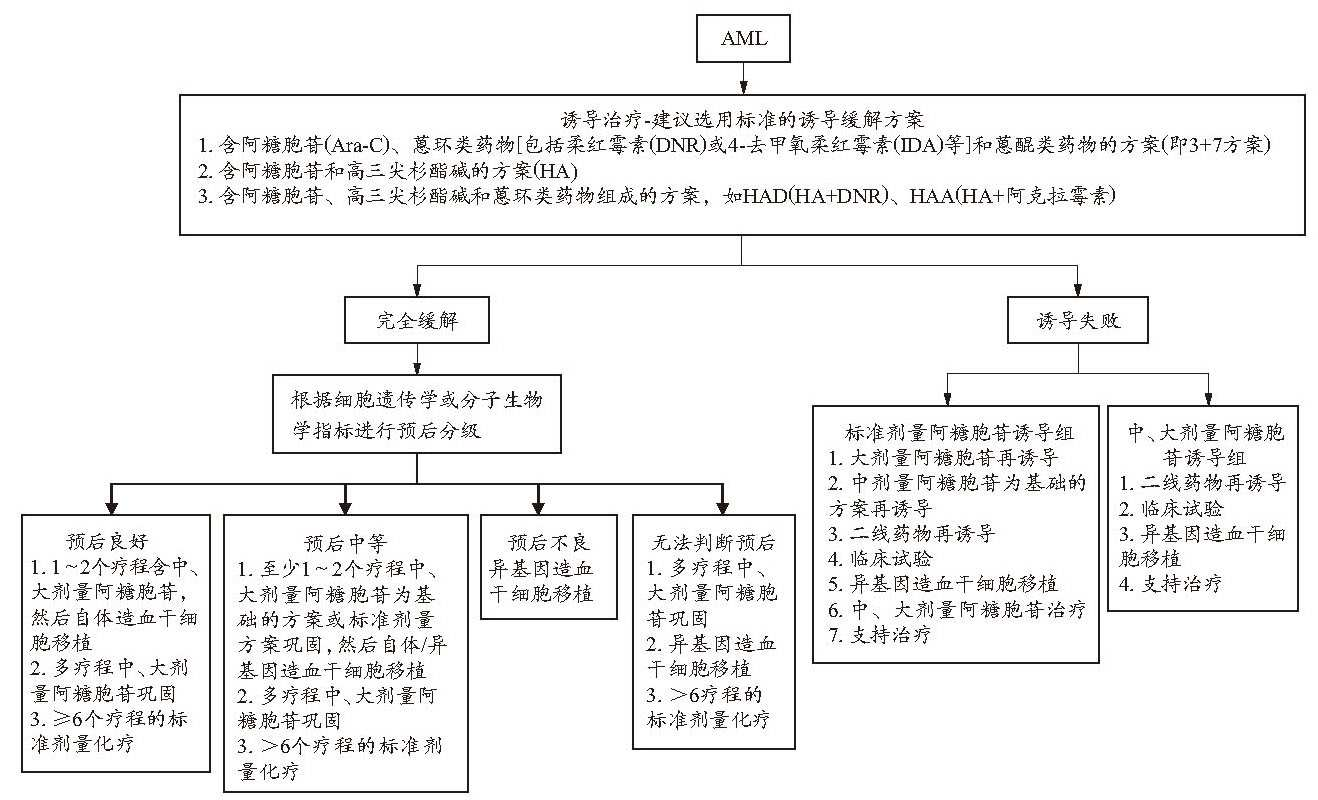
\includegraphics{./images/Image00141.jpg}
 \captionsetup{justification=centering}
 \caption{初诊年龄<60岁AML治疗程序}
 \label{fig5-1-8}
  \end{figure} 

\begin{figure}[!htbp]
 \centering
 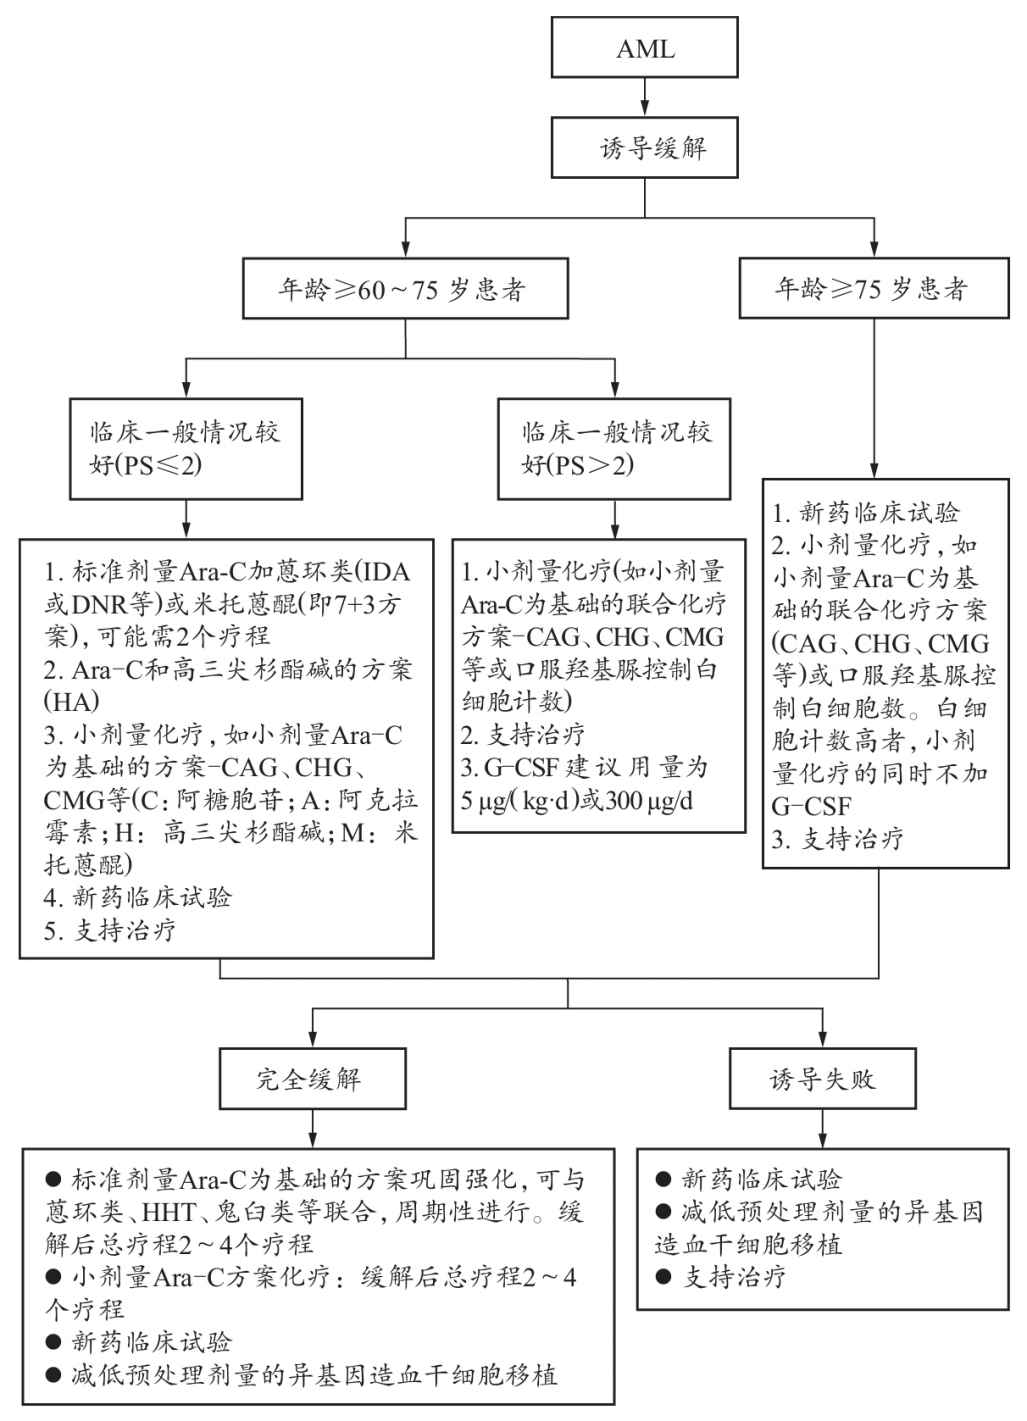
\includegraphics{./images/Image00142.jpg}
 \captionsetup{justification=centering}
 \caption{初诊年龄≥60岁APL治疗程序}
 \label{fig5-1-9}
  \end{figure} 

\begin{figure}[!htbp]
 \centering
 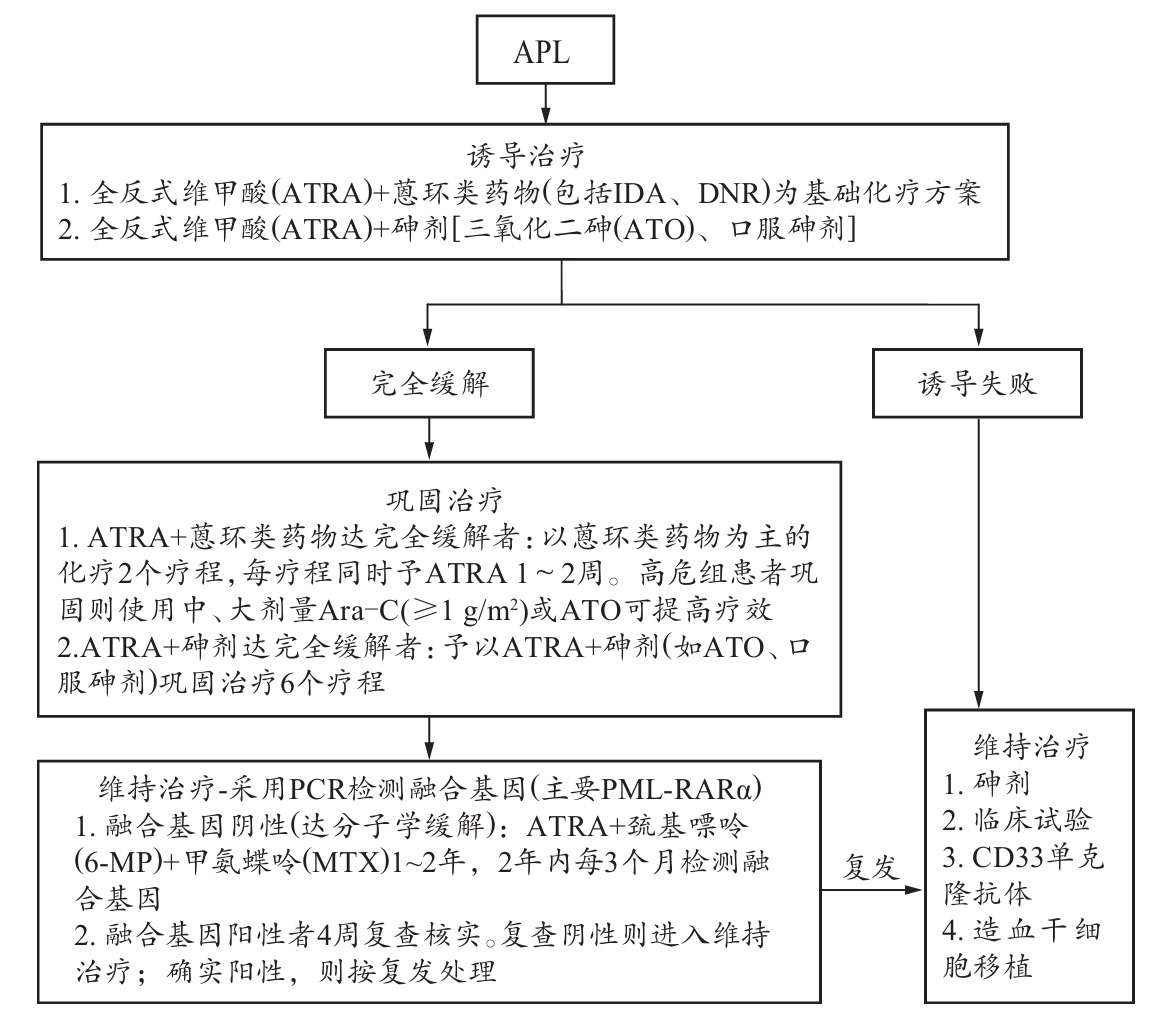
\includegraphics{./images/Image00143.jpg}
 \captionsetup{justification=centering}
 \caption{APL治疗程序}
 \label{fig5-1-10}
  \end{figure} 

\begin{figure}[!htbp]
 \centering
 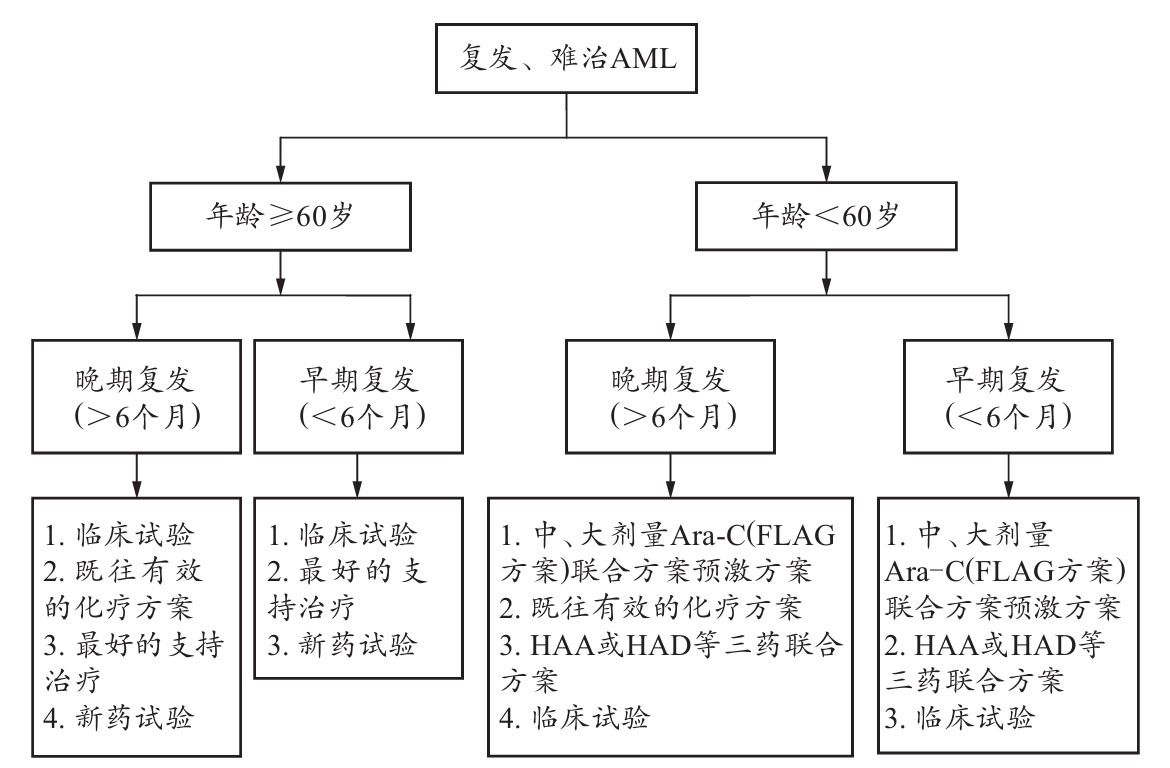
\includegraphics{./images/Image00144.jpg}
 \captionsetup{justification=centering}
 \caption{复发、难治AML治疗程序}
 \label{fig5-1-11}
  \end{figure} 

【治疗方案】

1. 支持治疗

(1)感染的防治:急性白血病患者常伴有粒细胞减少,而接受化疗、放疗后常出现持续而严重的缺乏,此时感染发生率高且严重。强调病房环境清洁,甚至住无菌层流病房,加强个人卫生和基础护理,减少探视。是否要预防性应用抗生素,无统一要求,国内外各个单位做法不一。如感染已存在,应做有关检查,以明确感染部位和性质,在致病菌查明之前,应立即给予联合广谱抗生素治疗。化疗后粒细胞减少患者,特别是老年患者,可以使用粒细胞集落刺激因子(G-CSF)5μg/(kg·d),直至ANC\textgreater{}1×10$^{9}$
/L。一般不主张白细胞输注。应注意的是G-CSF可能影响骨髓结果的解释,所以如要通过骨髓了解是否缓解,要求至少停止G-CSF7日后骨髓穿刺。

(2)贫血的治疗:如患者贫血较严重,需输注红细胞悬液,治疗过程中应保持患者Hb70~90g/L以上,有冠心病者应保持患者Hb100~120g/L以上。高白细胞白血病患者输血要慎重,以免进一步增加血粘度。最好输注去除白细胞的血液制品。氟达拉滨化疗后应输注辐照血(30Gy×30min),以防可能危及生命的输血相关的移植物抗宿主病(GVHD)。

(3)出血的防治:PLT<10×10$^{9}$
/L或有出血表现者,应输注单采血小板。如出血系弥散性血管内凝血(DIC)引起,则按DIC处理。对于APL伴发DIC,应尽量使血小板维持在50×10$^{9}$
/L以上,同时输注冷沉淀和新鲜冰冻血浆维持纤维蛋白原1.5g/L以上。

(4)高白细胞的治疗:高白细胞白血病由于白细胞淤滞危及生命,须紧急采取措施迅速降低白细胞。诱导治疗前常用羟基脲3~4g/d处理。也可应用血细胞分离机去除白细胞,使白细胞数<50×10$^{9}$
/L。因APL细胞的生物学特征与其他类型不同,建议一般不用血细胞分离机去除白细胞。

(5)防治尿酸性肾病及急性肿瘤溶解综合征(ATLS):高白细胞白血病,特别是对化疗敏感的患者,容易出现高尿酸血症、低钙血症、高磷血症和高钾血症为特征的ATLS,ATLS危及生命,所以对初诊急性白血病患者,均应积极防治ATLS。防治ATLS的基本措施为:①别嘌呤醇,300mg/d,降低尿酸;②化疗前及进行中充分补液水化、利尿并碱化尿液,可口服碳酸氢钠3.0g/d;③避免静脉造影检查和非甾体类抗炎药;④积极纠正可能发生的电解质紊乱;⑤有肾功能不全或急性肾衰竭征象者尽早肾内科会诊,必要时透析治疗。

(6)深静脉置管:建议AML患者行深静脉置管,由此进行药物和血液制品输注以及营养支持。这样可保证治疗顺利进行,同时减少了反复静脉穿刺给患者带来的痛苦。

2. 具体化疗方案

(1)DA方案:初治AML诱导治疗选用的标准剂量诱导方案

\begin{longtable}[]{|c|c|}
\toprule
\endhead
\vtop{\hbox{\strut 柔红霉素 45mg/(m$^2$ ·d)}\hbox{\strut NS 250ml}} &
静脉滴注,d1~3\tabularnewline
\bottomrule
\end{longtable}

\begin{longtable}[]{|c|c|}
\toprule
\endhead
\vtop{\hbox{\strut 阿糖胞苷 100~200mg/(m$^2$
·d)}\hbox{\strut NS 250ml}} &
持续静脉滴注,d1~7\tabularnewline
\bottomrule
\end{longtable}

(2)IA方案:初治AML诱导治疗选用的标准剂量诱导方案

\begin{longtable}[]{|c|c|}
\toprule
\endhead
\vtop{\hbox{\strut 去甲氧柔红霉素 8~12mg/(m$^2$
·d)}\hbox{\strut NS 250ml}} &
静脉滴注,d1~3\tabularnewline
\bottomrule
\end{longtable}

\begin{longtable}[]{|c|c|}
\toprule
\endhead
\vtop{\hbox{\strut 阿糖胞苷 100~200mg/(m$^2$
·d)}\hbox{\strut NS 250ml}} &
持续静脉滴注,d1~7\tabularnewline
\bottomrule
\end{longtable}

(3)HA方案:初治AML诱导治疗选用的标准剂量诱导方案

\begin{longtable}[]{|c|c|}
\toprule
\endhead
\vtop{\hbox{\strut 高三尖杉酯碱 3mg}\hbox{\strut NS 250ml}} &
静脉滴注,d1~7\tabularnewline
\bottomrule
\end{longtable}

\begin{longtable}[]{|c|c|}
\toprule
\endhead
\vtop{\hbox{\strut 阿糖胞苷 100~200mg/(m$^2$
·d)}\hbox{\strut NS 250ml}} &
静脉滴注,d1~7\tabularnewline
\bottomrule
\end{longtable}

(4)HAA方案:初治AML诱导治疗或复发及难治AML选用

\begin{longtable}[]{|c|c|}
\toprule
\endhead
\vtop{\hbox{\strut 高三尖杉酯碱 3mg}\hbox{\strut NS 250ml}} &
\vtop{\hbox{\strut 静脉滴注,每日2次,d1~3}\hbox{\strut 或每日1次,d1~7}}\tabularnewline
\bottomrule
\end{longtable}

\begin{longtable}[]{|c|c|}
\toprule
\endhead
\vtop{\hbox{\strut 阿糖胞苷 100~200mg/(m$^2$
·d)}\hbox{\strut NS 250ml}} &
静脉滴注,d1~7\tabularnewline
\bottomrule
\end{longtable}

\begin{longtable}[]{|c|c|}
\toprule
\endhead
\vtop{\hbox{\strut 阿克拉霉素 20mg}\hbox{\strut NS 250ml}} &
静脉滴注,d1~7\tabularnewline
\bottomrule
\end{longtable}

(5)HAD方案:初治AML诱导治疗或复发及难治AML选用

\begin{longtable}[]{@{}ccl@{}}
\toprule
\endhead
\vtop{\hbox{\strut 高三尖杉酯碱 3mg}\hbox{\strut NS 250ml}} &
静脉滴注,d1~7\tabularnewline
\bottomrule
\end{longtable}

\begin{longtable}[]{|c|c|}
\toprule
\endhead
\vtop{\hbox{\strut 阿糖胞苷 100~200mg/(m$^2$
·d)}\hbox{\strut NS 250ml}} &
静脉滴注,d1~7\tabularnewline
\bottomrule
\end{longtable}

\begin{longtable}[]{|c|c|}
\toprule
\endhead
\vtop{\hbox{\strut 柔红霉素 40mg/m$^2$}\hbox{\strut NS 250ml}} &
静脉滴注,d1~3\tabularnewline
\bottomrule
\end{longtable}

(6)MA方案:初治AML诱导治疗选用

\begin{longtable}[]{|c|c|}
\toprule
\endhead
\vtop{\hbox{\strut 米托蒽醌 10mg/m$^2$}\hbox{\strut NS 250ml}} &
静脉滴注,d1~3\tabularnewline
\bottomrule
\end{longtable}

\begin{longtable}[]{|c|c|}
\toprule
\endhead
\vtop{\hbox{\strut 阿糖胞苷 100~200mg/(m$^2$
·d)}\hbox{\strut NS 250ml}} &
持续静脉滴注,d1~7\tabularnewline
\bottomrule
\end{longtable}

(7)中剂量阿糖胞苷方案:AML巩固治疗选用

\begin{longtable}[]{|c|c|}
\toprule
\endhead
\vtop{\hbox{\strut 阿糖胞苷 1.0~2.0g/m$^2$}\hbox{\strut NS 250ml}}
&
\vtop{\hbox{\strut 持续2小时静脉滴注}\hbox{\strut 每12小时1次,共6~8次}}\tabularnewline
\bottomrule
\end{longtable}

(8)大剂量阿糖胞苷方案:AML巩固治疗选用

\begin{longtable}[]{|c|c|}
\toprule
\endhead
\vtop{\hbox{\strut 阿糖胞苷 3g/m$^2$}\hbox{\strut NS 250ml}} &
\vtop{\hbox{\strut 持续2小时静脉滴注}\hbox{\strut 每12小时1次,共6~8次}}\tabularnewline
\bottomrule
\end{longtable}

(9)FLAG方案:AML巩固治疗或复发及难治AML选用

\begin{longtable}[]{|c|c|}
\toprule
\endhead
\vtop{\hbox{\strut 氟达拉滨 30mg/m$^2$}\hbox{\strut NS 250ml}} &
持续30分钟静脉滴注,d1~5\tabularnewline
\bottomrule
\end{longtable}

\begin{longtable}[]{|c|c|}
\toprule
\endhead
\vtop{\hbox{\strut 阿糖胞苷 1~2g/m$^2$}\hbox{\strut NS 250ml}}
&
\vtop{\hbox{\strut 氟达拉滨开始后4小时应用}\hbox{\strut 持续4小时静脉滴注,d1~5}}\tabularnewline
\bottomrule
\end{longtable}

G-CSF 5μg/kg,皮下注射,d0~5或直至中性粒细胞\textgreater{}1.0×10$^{9}$
/L

(10)CAG方案:老年、复发及难治AML选用

阿糖胞苷 10mg/m$^2$ ,皮下注射,每12小时1次,d1~14

\begin{longtable}[]{|c|c|}
\toprule
\endhead
\vtop{\hbox{\strut 阿克拉霉素 10mg}\hbox{\strut NS 250ml}} &
静脉滴注,d1~8\tabularnewline
\bottomrule
\end{longtable}

G-CSF 200μg/m$^2$
,皮下注射,d1~14,外周血白细胞\textgreater{}20×10$^{9}$
/L停药

(11)初治老年(年龄\textgreater{}60岁)AML诱导治疗选用:

\begin{longtable}[]{|c|c|}
\toprule
\endhead
\vtop{\hbox{\strut 地西他滨 20mg/(m$^2$ ·d)}\hbox{\strut NS 250ml}} &
静脉滴注,维持1小时每4周1个疗程\tabularnewline
\bottomrule
\end{longtable}

(12)初治APL诱导治疗选用:

全反式维甲酸 45mg/(m$^2$ ·d),分2次口服,直至CR

(13)初治APL诱导治疗、APL复发选用:

\begin{longtable}[]{|c|c|}
\toprule
\endhead
\vtop{\hbox{\strut 三氧化二砷 0.15mg/kg}\hbox{\strut 5\%GS 500ml}} &
\vtop{\hbox{\strut 静脉滴注}\hbox{\strut 直至CR,最多60个剂量,注意毒副作用}}\tabularnewline
\bottomrule
\end{longtable}

(14)APL维持治疗选用:

全反式维甲酸 45mg/(m$^2$
·d),分2次口服,d1~15,每3个月1次

6-巯基嘌呤 50~100mg/m$^2$ ,口服,每日1次

甲氨蝶呤 10mg/m$^2$ ,口服或肌内注射,每周1次

3.
造血干细胞移植(HSCT) 对部分中等预后、高危及复发/难治急性白血病患者应选择各种类型的HSCT。

【疗效观察与随访】

1. 观察指标 常见症状与体征、血象、白细胞形态、骨髓常规等。

2. 疗效标准

(1)骨髓形态学无白血病状态:①由骨髓小粒骨髓穿刺提示骨髓原始细胞<5\%。②原始细胞中无Auer小体,无髓外病变。

(2)完全缓解(CR):患者获无白血病状态,并且:①ANC\textgreater{}1×10$^{9}$
/L。②PLT≥100×10$^{9}$
/L。③无髓外病变残留的证据。④形态学CR:患者无需输血。⑤细胞遗传学CR:细胞遗传学检查正常(初发时存在细胞遗传学异常)。⑥分子生物学CR:分子生物学检查阴性(目前仅在APL、Ph{+}
白血病证实有意义)。部分患者仅血小板未达标准者称为CRp。

(3)部分缓解(PR):原始细胞至少减少50\%,骨髓穿刺提示原始细胞占5\%~25\%。PR仅用来评估一些新药物的治疗效果,不可以作为标准治疗的疗效目标。

(4)难治性AML:①经典诱导治疗方案2个疗程未获CR。②CR1后6个月内复发。③CR1后6个月后复发,经正规诱导化疗失败。④2次及2次以上复发。⑤髓外白血病持续存在。

(5)复发:CR后外周血重新出现白血病细胞或骨髓原始细胞\textgreater{}5\%(除外其他原因巩固治疗后骨髓重建等)或髓外出现白血病细胞浸润。

3.
随访 诱导治疗过程中要观察化疗后第7日(骨髓抑制期)和第21日(血常规指标恢复期)骨髓象和血常规检查结果进行治疗方案的调整。

(1)标准剂量Ara-C诱导治疗患者:①化疗后第7日检查骨髓象:如果存在明显的残留白血病细胞(≥10\%),可考虑进行双诱导治疗。②化疗后第21日检查骨髓象和血常规,根据检查结果选择治疗方案:完全缓解,进入缓解后治疗。幼稚细胞比例下降不足60\%按诱导失败对待。未取得完全缓解,但幼稚细胞比例下降超过60\%可重复原方案1个疗程。增生低下,残留白血病细胞<10\%时等待恢复;残留白血病细胞≥10\%可考虑下一步治疗(参考双诱导治疗或按治疗失败对待)。

(2)含中、大剂量Ara-C诱导治疗患者:①化疗后第7日检查骨髓象和血常规,根据检查结果选择治疗方案。②化疗后第21日检查骨髓象和血常规,根据检查结果选择治疗方案。

(3)此外:主要病情观察,观察症状和体征等变化,可定期复查血常规、生化等检查;定期复查骨髓常规及细胞遗传学检查及分子生物学指标(如融合基因PML-RARα)。

【治疗经验与解析】

1.
良好的医患沟通是保证急性白血病治疗成功的重要因素。一旦诊断确立,应尽快向患者及其家属交代病情及其治疗,包括治疗疗效、治疗过程中的不良反应等,使患者及其家属理解并配合。医患沟通过程中,要根据患者的文化、宗教、习惯及性格等特点进行必要的保护性医疗。

2.
全反式维甲酸及砷剂治疗APL过程中可能发生危及生命的分化综合征,常与高白细胞相关、表现为发热、体重增加、呼吸困难、低血压、心包和胸腔积液、肺间质浸润及急性肾衰竭。一旦诊断明确,维甲酸应减量或停用直至上述症状消失,同时给予地塞米松20mg/d,分2次静脉滴注,连续3~5日,15日内逐渐停药,同时正规化疗。

3.
AML患者中枢神经系统白血病(CNSL)的发生率一般<3\%。参考NCCN的意见,不建议在诊断时即对无症状的患者行腰穿检查。有头痛、精神错乱的患者先行放射学检查,排除神经系统出血或感染。这些症状也可由白细胞淤滞引起,可通过白细胞分离等降低白细胞数量。若体征不清楚,无颅内出血的证据,可在纠正凝血紊乱和血小板支持的情况下行腰椎穿刺。而初诊时即有中枢神经系统症状且腰穿脑脊液发现白血病细胞以及CR1后腰穿检查阳性的患者需腰穿鞘注MTX8~12mg/m$^2$
±Ara-C30mg/m$^2$
+地塞米松2~5mg,每周2次,直至脑脊液正常,以后每周1次,4~6周。诊断时WBC\textgreater{}100×10$^{9}$
/L或单核细胞白血病(AML-M4、M5)的患者CR1后需腰穿鞘注MTX8~12mg/m$^2$
±Ara-C30mg/m$^2$ +地塞米松2~5mg,4~6次。

4.
大多数的AML不需要维持治疗,但APL是一个例外。APL在诱导巩固治疗后还需要进行维持治疗。

{(二)急性淋巴细胞白血病}
 急性淋巴细胞白血病(ALL)是一种发生在B细胞或T细胞系的未成熟淋巴细胞或淋巴祖细胞的肿瘤性疾病,原始细胞在骨髓中增殖和聚集,导致正常造血受到抑制,引起贫血、血小板减少和中性粒细胞减少。原始淋巴细胞可以累及多种髓外组织,如脑膜、性腺、胸腺、肝、脾和淋巴结等。

ALL是15岁以下患者中最常见的恶性肿瘤之一,占这个年龄组所有白血病的75\%,发病高峰在2~5岁,10岁以后发病率随年龄增长逐渐下降。在成人中15~24岁有一发病高峰,另一高峰出现于60岁以上的老年人。

【治疗程序】 如图\ref{fig5-1-12}所示。

\begin{figure}[!htbp]
 \centering
 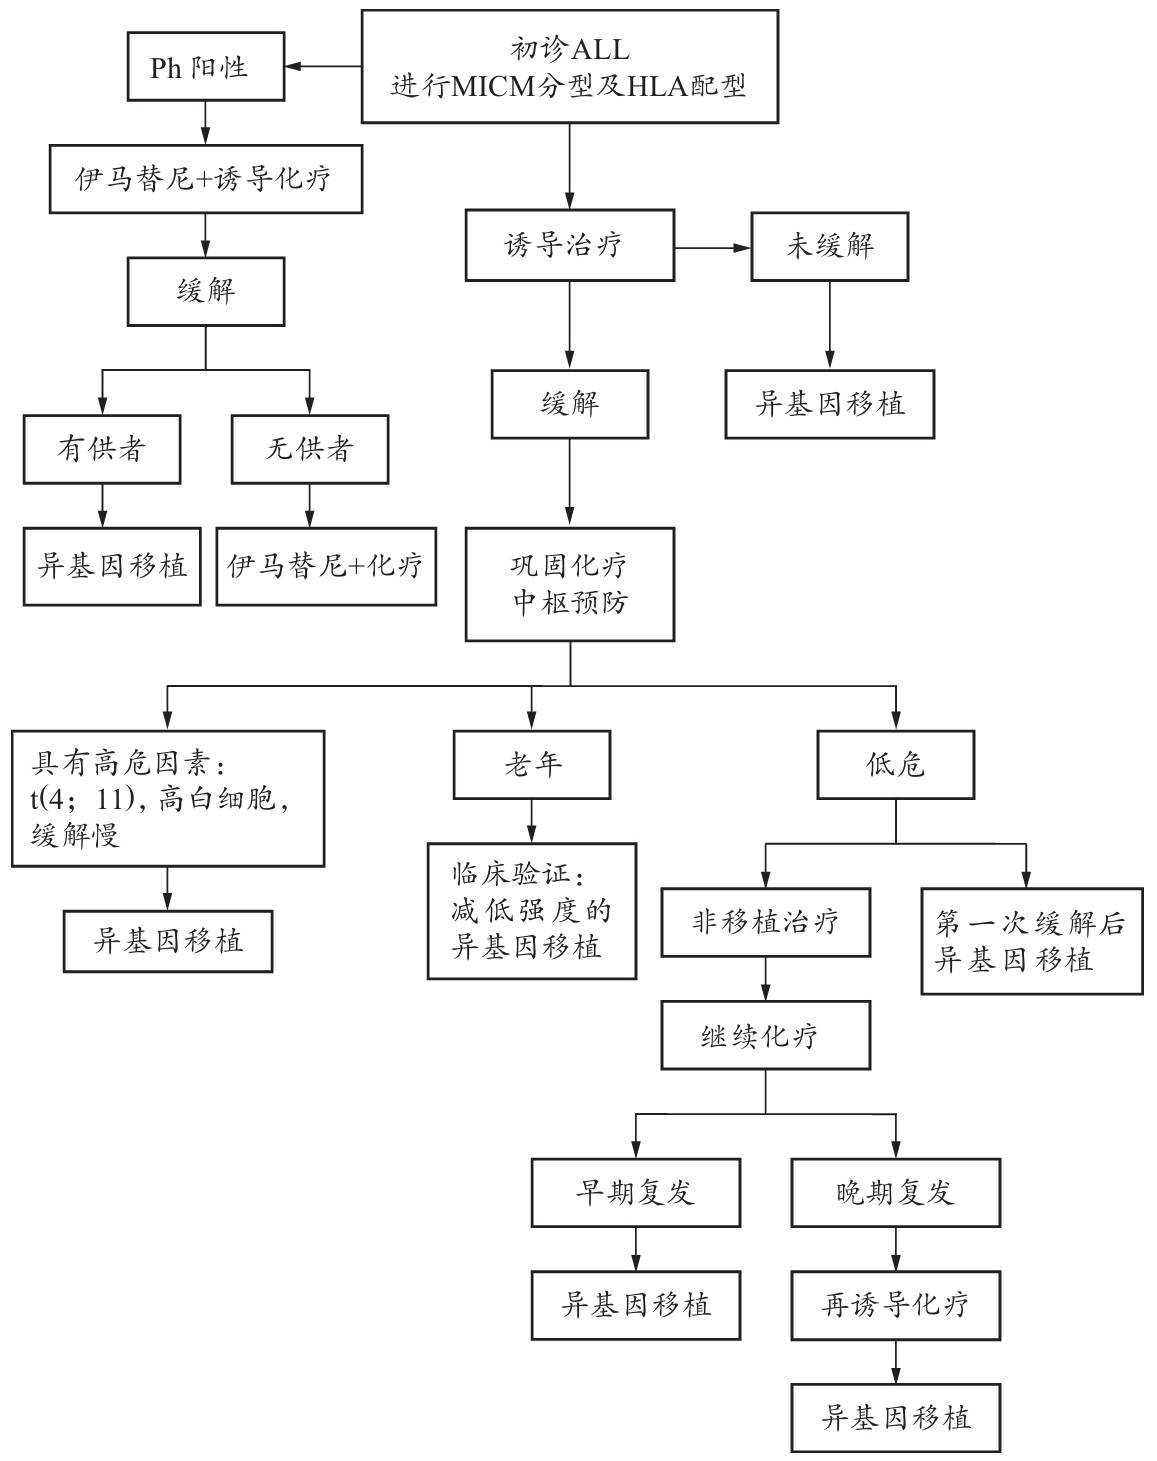
\includegraphics{./images/Image00145.jpg}
 \captionsetup{justification=centering}
 \caption{急性淋巴细胞白血病的治疗程序}
 \label{fig5-1-12}
  \end{figure} 

【治疗方案】 由于ALL是一种异质性疾病,应根据不同亚型的生物学特性选择个体化治疗方案。化疗是ALL最主要、最基本的治疗方法,分为两个阶段:第一阶段是诱导缓解治疗,目的是迅速、大量减少体内白血病细胞负荷,恢复正常造血,达到缓解;第二阶段为缓解后治疗(包括巩固强化治疗、维持治疗和中枢神经系统白血病的防治等),目的是消灭体内残存白血病细胞,预防复发、延长生存。

1. 治疗方案1 适用于除某些特殊类型(如Ph{+}
和Burkitt型)外的大多数成人ALL患者(“十一五”国家科技支撑计划成人ALL方案):

(1)预治疗:如果WBC≥50×10$^{9}$
/L,或者肝、脾、淋巴结肿大明显,则使用预治疗,以防止肿瘤溶解综合征的发生。

泼尼松(Pred) 60mg/d,口服,d-3~-1

环磷酰胺(CTX) 200mg/(m$^2$ ·d),静脉滴注,d-3~-1

(2)诱导治疗:VDCLP方案:

长春新碱(VCR) 2mg,静脉注射,d1,d8,d15,d22(1.4mg/m$^2$
,最大量不超过每次2mg)

柔红霉素(DNR) 40mg/(m$^2$
·d),静脉滴注,d1~3,d15~16(若d14骨髓有残留白血病细胞时使用,继续d15~16治疗,反之,则d15~16不治疗)

CTX 750mg/m$^2$ ,静脉滴注,d1,d15(美司钠解救)

左旋门冬酰氨酶(L-Asp),6000IU/m$^2$
,静脉滴注d11,d14,d17,d20,d23,d26

Pred 1mg/(kg·d),口服,d1~14;d15开始(d15~28)可以降低1/3的剂量用药

血象恢复后(WBC≥1×10$^{9}$ /L,PLT≥50×10$^{9}$ /L)进行鞘内注射(三联):

\begin{longtable}[]{@{}ll@{}}
\toprule
\endhead
\vtop{\hbox{\strut 甲氨蝶呤(MTX) 10mg}\hbox{\strut 阿糖胞苷(Ara-C) 50mg}\hbox{\strut 地塞米松(Dex) 5mg}}
& 鞘内注射2次,中间间隔至少3日。\tabularnewline
\bottomrule
\end{longtable}

有移植指征者,行HLA配型,寻找合适供体

挽救治疗:第28日缓解与否均进入下一步治疗。

(3)早期巩固强化治疗:

1)CAM(T)方案:

CTX 750mg/m$^2$ ,静脉滴注,d1,d8(美司钠解救)

Ara-C 100mg/(m$^2$
·d),静脉滴注,d1~3,d8~10

巯基嘌呤(6-MP或6-TG) 60mg/(m$^2$ ·d),口服,d1~7

血象恢复后,进行三联鞘内注射(见VDCLP方案)。

2)大剂量MTX+L-Asp方案:

MTX 3g/m$^2$  静脉滴注持续24小时,d1(T-ALL可加量至5g/m$^2$ )

\begin{longtable}[]{@{}ll@{}}
\toprule
\endhead
\vtop{\hbox{\strut MTX 10mg}\hbox{\strut Dex 5mg}} &
鞘内注射,d1\tabularnewline
\bottomrule
\end{longtable}

L-Asp 6000IU/m$^2$ ,静脉滴注,d3,d4

3)MA方案:

米托蒽醌(MIT) 6mg/(m$^2$ ·d),静脉滴注,d1~3

Ara-C 750mg/m$^2$ ,静脉滴注,q12h,d1~3

血象恢复后,进行三联鞘内注射(见VDCLP方案)

分层治疗:高危患者,有同胞相合、半相合或无关供体者,行异基因造血干细胞移植。无供体的患者继续下面治疗。

(4)晚期强化:

1)VDLP方案(再诱导治疗):

VCR 2mg,静脉注射,d1,d8,d15,d22

DNR 40mg/(m$^2$ ·d),静脉滴注,d1~3

L-Asp 6000IU/m$^2$ ,静脉滴注,d11,d14,d17,d20,d23,d26

DEX 8mg/(m$^2$
·d),口服或静脉滴注,d1~7,d15~21

血象恢复后,进行三联鞘内注射(见VDCLP方案)。

2)COATD方案:

CTX 750mg/m$^2$ ,静脉滴注,d1

VCR 2mg,静脉注射,d1

Ara-C 100mg/(m$^2$ ·d),静脉滴注,d1~7

VM-26 100mg/(m$^2$ ·d),静脉滴注,d1~4

DEX 6mg/(m$^2$ ·d),口服或静脉滴注,d1~7

(头颅和脊髓照射的患者,Ara-C和VM-26均减1日)

血象恢复,进行鞘内注射(见VDCLP方案)。

分层治疗:无合适供体的高危组患者、标危组患者可以考虑进行自体造血干细胞移植。无移植条件的患者继续下面治疗。

3)大剂量MTX+L-Asp方案:

MTX 3g/m$^2$ ,静脉滴注持续24小时,d1(T-ALL可加量至5g/m$^2$ )

L-Asp 10000IU,静脉滴注,d3,d4(MTX输注结束24h后)

\begin{longtable}[]{@{}ll@{}}
\toprule
\endhead
\vtop{\hbox{\strut MTX 10mg}\hbox{\strut Dex5mg}} &
鞘内注射,d1(已行颅脑照射的患者不再鞘注)\tabularnewline
\bottomrule
\end{longtable}

4)TA方案:

VM-26 100mg/(m$^2$ ·d),静脉滴注,d1~4

Ara-C 100mg/(m$^2$ ·d),静脉滴注,d1~7

血象恢复后,进行鞘内注射(见VDCLP方案)。

(5)中枢神经系统白血病(CNSL)预防治疗:18岁以上的高危组患者一般应考虑进行颅脑分次(10~12次)照射,总量18~20Gy;有CNSL的证据者照射剂量为24Gy,照射野为颅脑+脊髓。标危组患者可以酌情进行。18岁以下的患者,未诊断CNSL时可以不进行头颅放疗。

放疗期间可予Pred口服或VP(VCR+Pred)方案维持(用法见VDCLP方案)。

已行颅脑照射的患者,若无CNSL的证据则半年内不进行鞘内注射治疗。

(6)维持治疗:每月1个疗程,直至缓解后3年。每6个月予强化治疗1次;维持治疗期间尽量保证3个月复查1次。

6-MP 60mg/(m$^2$ ·d),口服,d1~7

MTX 20mg/(m$^2$ ·d),口服,d8

(7)强化治疗(维持治疗时应用):MOACD方案:

MIT 8mg/(m$^2$ ·d),静脉滴注,d1,d2

VCR 2mg,静脉注射,d1

CTX 600mg/m$^2$ ,静脉滴注,d1

Ara-C 100mg/(m$^2$ ·d),静脉滴注,d1~5

DEX 6mg/(m$^2$ ·d),口服或静脉滴注,d1~7

高危组、未行头颅照射的患者,每6个月强化的同时鞘注1次。

共鞘注12次(低危组)~16次(高危组),L-Asp总应用次数16次左右。

附:大剂量MTX的应用及四氢叶酸钙的解救(表\ref{tab5-1-3})。

表\ref{tab5-1-3} MTX浓度与四氢叶酸钙剂量

\begin{longtable}[]{@{}ll@{}}
\toprule
\endhead
MTX浓度(μmol/L) & 四氢叶酸钙(mg/m$^2$ )\tabularnewline
1~2 & 30\tabularnewline
2~3 & 45\tabularnewline
3~4 & 60\tabularnewline
4~5 & 75\tabularnewline
\textgreater{}5 & MTX浓度×体重(kg)\tabularnewline
\bottomrule
\end{longtable}

MTX 3g/m$^2$
,1/3量30分钟内输入(此时行腰穿鞘注MTX,以提高脑脊液中MTX的浓度),余量维持23小时,静脉滴注,d1。

停药12小时开始解救,四氢叶酸钙用量30mg/(m$^2$
·次),6小时1次,解救至MTX浓度<0.1μmol/L(若不能监测MTX浓度,则根据口腔粘膜损伤情况解救6~8次)。

若在第42h或48h时(自MTX用药计算时间)MTX浓度高于下述值,四氢叶酸钙剂量应进行调整。

2. 治疗方案2 适用于成人Ph{+}
ALL患者(“十一五”国家科技支撑计划成人ALL方案)。

(1)预治疗:同治疗方案1。

(2)诱导治疗:

VDCP方案:

VCR 2mg,静脉注射,d1,d8,d15,d22(1.4mg/m$^2$
,最大量不超过2mg/次);

DNR 40mg/m$^2$
,静脉滴注,d1~3,d15(若d14骨髓有残留白血病细胞,继续d15治疗,反之,则d15不治疗);

CTX 750mg/m$^2$ ,静脉滴注,d1,d15(美司钠解救);

Pred 1mg/(kg·d),口服,d1~14;d15开始(d15~28)可以降低1/3的剂量用药。

血象恢复后进行鞘内注射同治疗方案1中VDCLP方案。

诱导治疗的前2周所有ALL患者基本一样(不管Ph/BCR-ABL阳性与否),在诱导治疗的第2周行骨髓穿刺,根据骨髓结果进行分层。Ph/BCR-ABL阳性患者进入Ph{+}
ALL治疗系列,自第15日开始加用伊马替尼,并尽量持续应用至维持治疗结束(无条件应用伊马替尼的患者按一般ALL的治疗方案进行,维持治疗改为干扰素)。

伊马替尼用药开始剂量400mg/日,并持续应用。若粒细胞缺乏(尤其是<0.2×10$^{9}$
/L)持续时间较长(超过1周),出现感染发热时,可以临时停药,以减少患者的风险。

于诱导化疗结束时(约为治疗的第4周左右)复查骨髓常规和细胞遗传学、BCR/ABL融合基因。有干细胞移植条件者,行HLA配型,寻找合适供体。

(3)早期巩固强化治疗:

1)CAM(T)方案:同治疗方案1。

2)大剂量MTX方案±VD:

MTX 3g/m$^2$ ,静脉滴注持续24小时,d1

\begin{longtable}[]{@{}ll@{}}
\toprule
\endhead
\vtop{\hbox{\strut MTX 10mg}\hbox{\strut Dex 5mg}} &
鞘内注射d1\tabularnewline
\bottomrule
\end{longtable}

VCR 2mg,静脉注射,d8

Dex 6mg/(m$^2$ ·d),口服或静脉滴注,d8~15

3)MA方案:

MIT 6mg/(m$^2$ ·d),静脉滴注,d1~3

Ara-C 100mg/(m$^2$ ·d),静脉滴注,d1~5

血象恢复后,进行三联鞘内注射同治疗方案1中VDCLP方案。

已找到骨髓供体,准备行干细胞移植者,伊马替尼持续口服至行造血干细胞移植(估计用药周期为5~6个月)。在治疗过程中,每疗程均监测BCR/ABL融合基因水平,有继续下降趋势的可在完成3个疗程的强化治疗后行干细胞移植;若融合基因表达呈上升趋势则直接进行移植。

造血功能重建后(如移植后1个月)复查染色体核型和BCR/ABL融合基因。若融合基因连续3次为零(阴性)则不再应用伊马替尼;否则,予伊马替尼口服(400mg/d)(至融合基因转阴性,连续复查2次阴性/每2个月1次)。伊马替尼的治疗时间为2~6个月。

无供体、无条件或其他原因不能行干细胞移植治疗者,继续接受巩固强化化疗和伊马替尼的联合治疗。

伊马替尼根据个人经济能力决定,无应用条件者按计划化疗,化疗结束后予干扰素维持治疗。

(4)CNSL预防治疗:未行干细胞移植的18岁以上患者一般应考虑进行颅脑分次(10~12次)照射,总量18~20Gy。有CNSL的证据者照射剂量为24Gy,照射野为颅脑+脊髓。照射期间可予Pred口服或VP(VCR+Pred)方案维持(用法见VDCLP方案)。

已行颅脑照射的患者,若无CNSL的证据则半年内不进行鞘注治疗。

(5)晚期强化:

1)COATD方案:

CTX 750mg/(m$^2$ ·d),静脉滴注,d1(美司钠解救)

VCR 2mg,静脉注射,d1

Ara-C 100mg/(m$^2$ ·d),静脉滴注,d1~5

VM-26 100mg/(m$^2$ ·d),静脉滴注,d1~4

DEX 8mg/(m$^2$ ·d),口服或静滴,d1~7

血象恢复后,进行三联鞘内注射(用法见VDCLP方案)。

2)VDCD方案:

VCR 2mg,静脉注射,d1,d8,d15,d22

DNR 40mg/(m$^2$ ·d),静脉滴注,d1~3

CTX 750mg/m$^2$ ,静脉滴注,d1,d15(美司钠解救)

DEX 6mg/(m$^2$
·d),口服或静脉滴注,d1~7,d15~21

血象恢复后,进行三联鞘内注射(用法见VDCLP方案)。

分子学阴性的患者可选择自体造血干细胞移植,移植后的患者继续可予伊马替尼(无条件者用干扰素)维持治疗,不再进行下面2个疗程治疗。

3)大剂量MTX方案±VD:

MTX 3g/m$^2$ ,静脉滴注持续24小时,d1

\begin{longtable}[]{@{}ll@{}}
\toprule
\endhead
\vtop{\hbox{\strut MTX 10mg}\hbox{\strut Dex 5mg}} &
鞘内注射d1(已行颅脑照射的患者不再鞘注)\tabularnewline
\bottomrule
\end{longtable}

VCR 2mg,静脉注射,d8

Dex 6mg/(m$^2$ ·d),口服或静脉滴注,d8~15

血象恢复后,进行三联鞘内注射(用法见VDCLP方案)。

4)TA方案:

VM-26 100mg/(m$^2$ ·d),静脉滴注,d1~4

Ara-C 100mg/(m$^2$ ·d),静脉滴注,d1~7

血象恢复后,进行三联鞘内注射(用法见VDCLP方案)。

(6)维持治疗(不能应用伊马替尼作为维持治疗者):采用干扰素维持治疗,300万U/次,qod,至缓解后3年。

疗效观察指标(维持治疗期间应尽量保证3个月复查1次):定期查血常规、骨髓象、染色体核型[t(9;22)]和(或)融合基因(BCR/ABL)。

3.
治疗方案3 适用于成熟B(Burkitt型)成人ALL患者:(Hyper-CVAD/MTX-Ara-C方案)。

(1)Hyper-CVAD(第1,3,5,7疗程):

CTX 300mg/m$^2$
,静脉滴注,持续3小时,q12h,d1~3(共6次)

美司钠(Mesna) 600mg/m$^2$ ,静脉滴注,持续24小时,d1~3

(与CTX同时开始,至最后1次CTX结束后6小时停止)

多柔比星(ADM) 50mg/m$^2$ ,静脉滴注,持续24小时,d4

VCR 2mg,静脉注射,d4,d11

Dex 40mg/d,静脉滴注,d1~4,d11~14

(2)MTX+大剂量Ara-C(第2,4,6,8疗程):

MTX 200mg/m$^2$ ,静脉持续2小时,MTX 800mg/m$^2$
,静脉滴注,持续22小时,d1

四氢叶酸钙 30mg/m$^2$ ,静脉滴注,q6h

(MTX停药12小时开始解救至MTX浓度<0.1μmol/L,若不能监测MTX浓度,则根据口腔粘膜损伤情况解救6~8次)

Ara-C 3g/m$^2$ (≥60岁患者1g/m$^2$
),静脉滴注持续2小时,q12h,d2,d3(共4次)

(3)CNSL预防和治疗:

甲氨蝶呤(MTX) 10mg,鞘内注射,d2

阿糖胞苷(Ara-C) 100mg,鞘内注射,d8

· CNSL:鞘内注射每周2次直至CNS阴性,然后继续预防治疗。

·
高危患者[LDH\textgreater{}600U/L和(或)高增殖指数;成熟B细胞ALL]:以上预防方案贯穿于全部8个疗程。

· 低危患者(无以上高危因素):以上预防方案用于前2个疗程。

· 未知危险组患者:以上预防方案用于前4个疗程。

4.
治疗方案4 适用于成熟B细胞(Burkitt型)成人ALL患者(“十一五”国家科技支撑计划成人ALL方案)。

(1)预治疗:如果WBC≥25×10$^{9}$
/L或者肝脾大、淋巴结肿大明显,则进行预治疗,以防止肿瘤溶解综合征的发生。

Pred 60mg/d,口服,d-5~-1

CTX 200mg/(m$^2$ ·d),静脉滴注,d-5~-1

(2)A方案(第1,7,13周应用)(第1,3,5,7疗程):

\begin{longtable}[]{@{}ll@{}}
\toprule
\endhead
\vtop{\hbox{\strut 甲氨蝶呤(MTX) 10mg}\hbox{\strut 阿糖胞苷(Ara-C) 50mg}\hbox{\strut 地塞米松(Dex) 5mg}}
& 鞘内注射 d1\tabularnewline
\bottomrule
\end{longtable}

利妥昔单抗(美罗华) 375mg/(m$^2$
·d),静脉滴注,d0(根据患者经济情况应用)

VCR 2mg,静脉注射,d1

MTX 1500mg/m$^2$ ,静脉滴注,持续24小时,d1

异环磷酰胺(IFO) 800mg/m$^2$
,静脉滴注,d1~5(美司钠解救)

VM-26 100mg/m$^2$ ,静脉滴注,d4,d5

Ara-C 150mg/m$^2$ ,静脉滴注,q12h,d4,d5

Dex 10mg/(m$^2$ ·d),口服或静脉滴注,d1~5

(3)B方案(第4,10,16周实施)(第2,4,6,8疗程):

\begin{longtable}[]{@{}ll@{}}
\toprule
\endhead
\vtop{\hbox{\strut 甲氨蝶呤(MTX) 10mg}\hbox{\strut 阿糖胞苷(Ara-C) 50mg}\hbox{\strut 地塞米松(Dex) 5mg}}
& 鞘内注射d1\tabularnewline
\bottomrule
\end{longtable}

利妥昔单抗(美罗华) 375mg/(m$^2$
·d),静脉滴注,d0(根据患者经济情况应用)

VCR 2mg,静脉注射,d1

MTX 1500mg/m$^2$ ,静脉滴注,持续24小时,d1

CTX 200mg/(m$^2$ ·d),静脉滴注,d1~5

多柔比星(ADM) 25mg/m$^2$ ,静脉滴注,d4,d5

Dex 10mg/(m$^2$ ·d),口服或静脉滴注,d1~5

(4)CNSL预防和治疗:

1)

\begin{longtable}[]{@{}ll@{}}
\toprule
\endhead
\vtop{\hbox{\strut 甲氨蝶呤(MTX) 10mg}\hbox{\strut 阿糖胞苷(Ara-C) 50mg}\hbox{\strut 地塞米松(Dex) 5mg}}
& 鞘内注射\tabularnewline
\bottomrule
\end{longtable}

2)放疗:20~24Gy分次放疗,于治疗4个疗程后进行,如无CNS累及,照射野仅为颅脑;如有CNS受累,照射野包括颅脑、脊髓。

放疗期间可予Pred口服或VP(VCR+Pred)方案维持(用法见VDCLP方案);放疗后的2疗程内大剂量MTX用药时不再鞘注。

5.
治疗方案5 适用于老年(≥60岁)ALL患者,体能状况差,合并心、肝、肾等基础疾患或功能不全时,不能耐受标准化疗。目前尚无针对老年ALL较为公认的疗效满意的化疗方案,以下“Age-adapted
Therapy”方案供参考:

(1)诱导缓解:

VCR 2mg,静脉注射,d1,d8,d15,d22

CTX 400mg/(m$^2$ ·d),静脉滴注,d1,d8,d15,d22

Pred 60mg/(m$^2$ ·d),口服,qod,d1~22

DNR 30mg/(m$^2$ ·d),d1,d8,d15,d22

d15骨髓原始细胞低于20\%,d15和d22不用DNR。

d28复查骨髓达CR,d35开始以下巩固治疗;若未达CR,则立即开始以下巩固方案作为挽救治疗。

(2)巩固治疗:

DNR 40mg/m$^2$ ,d1

Ara-C 60mg/(m$^2$ ·d),肌内注射或静脉滴注,d1~5

L-Asp 500U/(kg·d),肌内注射或静脉滴注,d6~10

若挽救治疗后达CR,再重复以上巩固方案1疗程。

(3)维持治疗(持续2年):

MTX 6mg/m$^2$ ,肌内注射,qw

6-MP 20mg/(m$^2$ ·d),口服,qd

IFNα-2b 3MU/m$^2$ ,皮下注射,tiw

根据血液学毒性调整剂量。

(4)CNSL的预防:鞘内注射在诱导缓解、巩固治疗期间各2次,维持治疗期间1次(用法见VDCLP方案)。

(5)老年Ph{+} ALL:加用伊马替尼治疗可明显改善预后。

【疗效观察与随访】

1.
观察指标 常规症状与体征、血象、白细胞形态、骨髓常规、血清淀粉酶、血糖等。

2. 疗效评估

(1)完全缓解(CR):

1)临床无白血病细胞浸润所致的症状和体征,生活正常或接近正常。

2)血象:Hb≥100g/L(男),或≥90g/L(女及儿童),ANC≥1.5×10$^{9}$
/L,PLT≥100×10$^{9}$ /L。外周血白细胞分类中无白血病细胞。

3)骨髓象:原粒细胞Ⅰ型+Ⅱ型(原始单核+幼稚单核细胞或原始淋巴+幼稚淋巴细胞)≤5\%,红细胞及巨核细胞系正常。

(2)部分缓解(PR):骨髓原粒细胞Ⅰ型+Ⅱ型(原始单核+幼稚单核细胞或原始淋巴+幼稚淋巴细胞)\textgreater{}5\%而≤20\%;或临床、血象中有一项未达完全缓解标准者。

3.
随访 密切观察病情变化,每3个月复查骨髓象1次,按病情变化不断调整治疗。

【治疗经验与解析】

1.
在化疗(尤其是应用L-Asp)的过程中若出现肝功能、出凝血等异常或严重感染,应酌情调整治疗。在应用L-Asp前需要确认患者肝功能、凝血功能、血清淀粉酶是否在正常范围,用药前及用药过程中无油饮食。

2.
老年患者应用L-Asp,相比较于其他年龄组,更易引起认知障碍、脑病,易被误诊为老年抑郁症或病毒性脑炎,要引起注意。

3.
应用蒽环类药物,特别是老年患者或有心脏基础病变时应充分考虑其心脏毒副作用。

4.
糖皮质激素可致高血糖、加重糖尿病、易感染、导致体液和电解质紊乱,对于老年患者和既往有相关基础疾病者要特别重视。

5. VCR可能引起严重便秘,可适当应用轻泻药予以预防。

6.
老年患者因其他非严重性的慢性病长期服用的药物,如有可能,在化疗期间尽量停用,以避免严重的药物间相互作用。

{(三)少见类型的白血病}

\paragraph{多毛细胞白血病}

多毛细胞白血病(HCL)是一种罕见的慢性B淋巴细胞增殖性疾病(B-LPD),在所有淋巴细胞白血病中约占2\%。1958年,由Bouroncle等首次描述,最早被称为白血病性网状内皮组织增生症。HCL主要特征为外周血和(或)骨髓存在有典型的多毛细胞(HC)、全血细胞减少和不同程度的脾肿大。HCL患者中位年龄55岁,但是诊断时年龄跨越范围较广。男性多见,男女比为(3~4)∶1。HCL的病因目前尚不清楚,且存在争议。有报道其发病具有家族倾向性,也有提出与病毒感染有关。通过免疫学、细胞遗传学和分子生物学研究提示毛细胞来源于B细胞。

【治疗程序】 HCL患者的治疗具有明显异质性,目前还缺乏较为统一的治疗意见。脾脏切除、IFN-α单药应用曾是HCL治疗的主要措施。20世纪90年代后嘌呤类药物成为治疗HCL的一线药物。利妥昔单抗也可获得显著疗效。治疗程序如图\ref{fig5-1-13}所示。

\begin{figure}[!htbp]
 \centering
 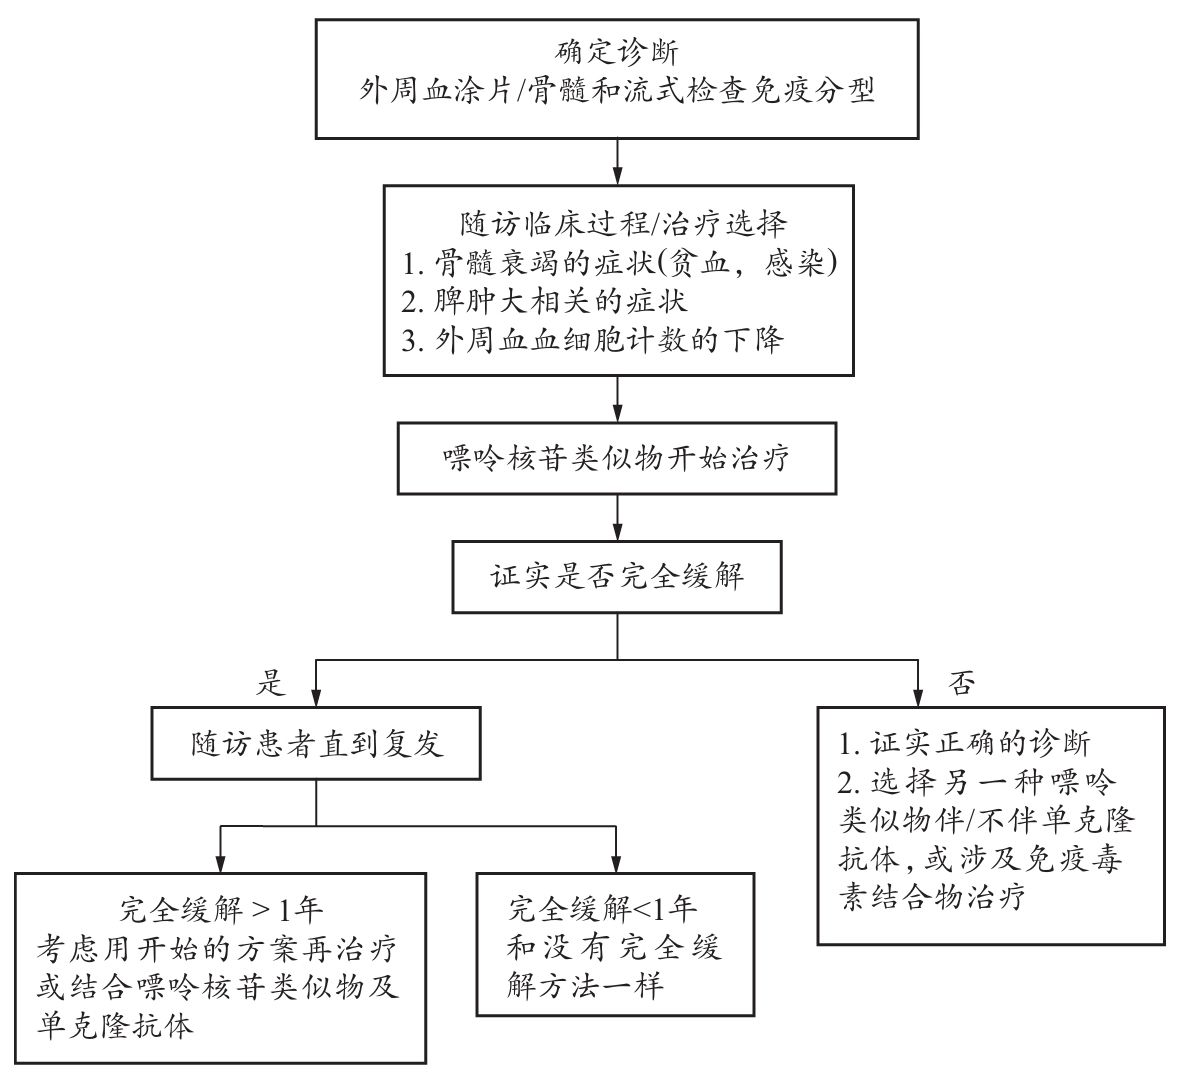
\includegraphics{./images/Image00146.jpg}
 \captionsetup{justification=centering}
 \caption{多毛细胞白血病的治疗程序}
 \label{fig5-1-13}
  \end{figure} 

【治疗方案】

1.
治疗指征 HCL呈惰性病程,进展缓慢,很多患者无需立即治疗,治疗指征包括:①有影响正常活动的症状如乏力、发热、盗汗等。②肝脾肿大或淋巴结肿大出现症状。③血红蛋白<120g/L,或需输血。④血小板<100×10$^{9}$
/L,或有出血。⑤白细胞\textgreater{}20×10$^{9}$
/L或HC增多。⑥中性粒细胞<1×10$^{9}$
/L。⑦伴有自身免疫性疾病。⑧反复或严重感染。

2. 药物治疗

(1)嘌呤类药物:

1)克拉屈滨:为HCL的一线治疗方案,给药方式多样,主要分三种:①0.14mg/(kg·w)×5w,CI
2小时;②0.14mg/(kg·d)×5d,CI 2小时;③0.1mg/(kg·d)×7d,CI
24小时。其中方案①更适于发病时伴中粒细胞减少的患者。

2)喷司他丁:早期研究显示其有较高的完全缓解率,超过85\%。一般用量4mg/m$^2$
,静脉滴注,每周或每2周1次,2个疗程,可有血液学改善,2个月内可恢复正常。

(2)α干扰素(IFN-α):在重度血细胞减少和嘌呤类药物治疗无效者可用,对典型的HCL疗效较好。治疗剂量一般为3MU/d或每周5日,或2~3MU/m$^2$
,每周3次,连用6~12个月,43\%CR,90\%PR。停药后2年内50\%可临床复发,复发后再用多数患者仍有效。

(3)脾脏切除:是HCL传统的标准治疗措施,也是化疗药物面世前唯一有效的治疗方法,一直沿用至20世纪80年代。由于HCL患者均有程度不一的血细胞减少,且大多和脾大有关。切脾后90\%患者血象可很快改善,40\%~70\%三系血细胞可恢复正常,惟独不能减少骨髓中的HC。疗程可维持18个月,5年生存率为70\%。目前已很少行脾切除术。切除指征:①巨脾疼痛或脾破裂。②脾大伴严重血小板减少和活动性出血。③活动或不能控制的感染。④化疗失败。

(4)利妥昔单抗:HC表面表达CD20,因此抗CD20的嵌合型单克隆抗体美罗华成为该疾病治疗药物之一。针对复发难治的毛细胞白血病患者,使用美罗华完全缓解(CR)率达13\%~53\%;对于毛细胞白血病变异型同样存在很好的疗效。虽然克拉屈滨和喷司他丁明显提高了该疾病患者的预后,但随访5年仍有20\%~30\%的患者复发。美罗华联合嘌呤类似物治疗其他淋巴增殖性疾病取得很好的临床效果,如FCR方案治疗CLL,因此美罗华联合克拉屈滨也同样可成为该疾病治疗策略之一。

【疗效观察与随访】

1. 观察指标 常见症状与体征,血象、骨髓活检、流式检测MRD等。

2. 疗效评估

(1)完全缓解(CR):症状与体征完全消失,血象恢复正常(血红蛋白≥120g/L,中性粒细胞绝对值≥1.5×10$^{9}$
/L,血小板≥100×10$^{9}$
/L,稳定至少1个月);外周血及骨髓中HC消失或HC<0.5(50\%);BM活检无HCL证据,网状纤维恢复正常。然而,最精细的是检查MRD。MRD定义为在不存在形态学的标准时,使用免疫分型分析,免疫组化染色或DNA聚合酶链反应来检测治疗后的HCL。

(2)部分缓解(PR):以上各项均有改善,但未恢复正常,血象三系细胞应有二系恢复正常;外周血及骨髓中HC减少≥0.5(50\%)。

(3)进步:以上各项指标有进步。血象三系细胞至少一系恢复正常;外周血及骨髓中HC减少<0.5(50\%)。

(4)无反应(NR):以上各项指标均未恢复正常。

3.
随访 主要观察症状和体征等变化,按疗效标准可定期复查血常规,观察血红蛋白、中性粒细胞、血小板的恢复情况,观察外周血及骨髓中多毛细胞的比例,定期复查骨髓活检、流式检测MRD等。

【治疗经验与解析】 骨髓增生程度对治疗方案的选择很重要,增生极度低下的患者需减少初始使用嘌呤类似物的剂量,避免延长和加重治疗相关骨髓抑制。克拉屈滨和喷司他丁均需监测肾功能。喷司他丁适用于血清肌酐<1.5mg/d的患者。使用喷司他丁治疗时需要以每单位剂量1.5L的液体充分的水化。如果患者血清肌酐值超过基线的20\%,需停止用药至肾功能恢复。

\paragraph{幼淋巴细胞白血病}

幼淋巴细胞白血病(PLL)是一种幼稚淋巴细胞的血液系统恶性疾病,主要累及外周血、骨髓及脾等淋巴器官,外周血中幼稚淋巴细胞占淋巴细胞≥55\%。PLL包括B-PLL及T-PLL二种亚型。从2001年始WHO分型取消了T细胞慢性淋巴细胞白血病(T-CLL),将其归入T-PLL。PLL约占所有成熟淋巴细胞白血病的2\%,男性多于女性,发病中位年龄65~70岁,呈侵袭性病程、预后差。

【治疗程序】 如图\ref{fig5-1-14}所示。

\begin{figure}[!htbp]
 \centering
 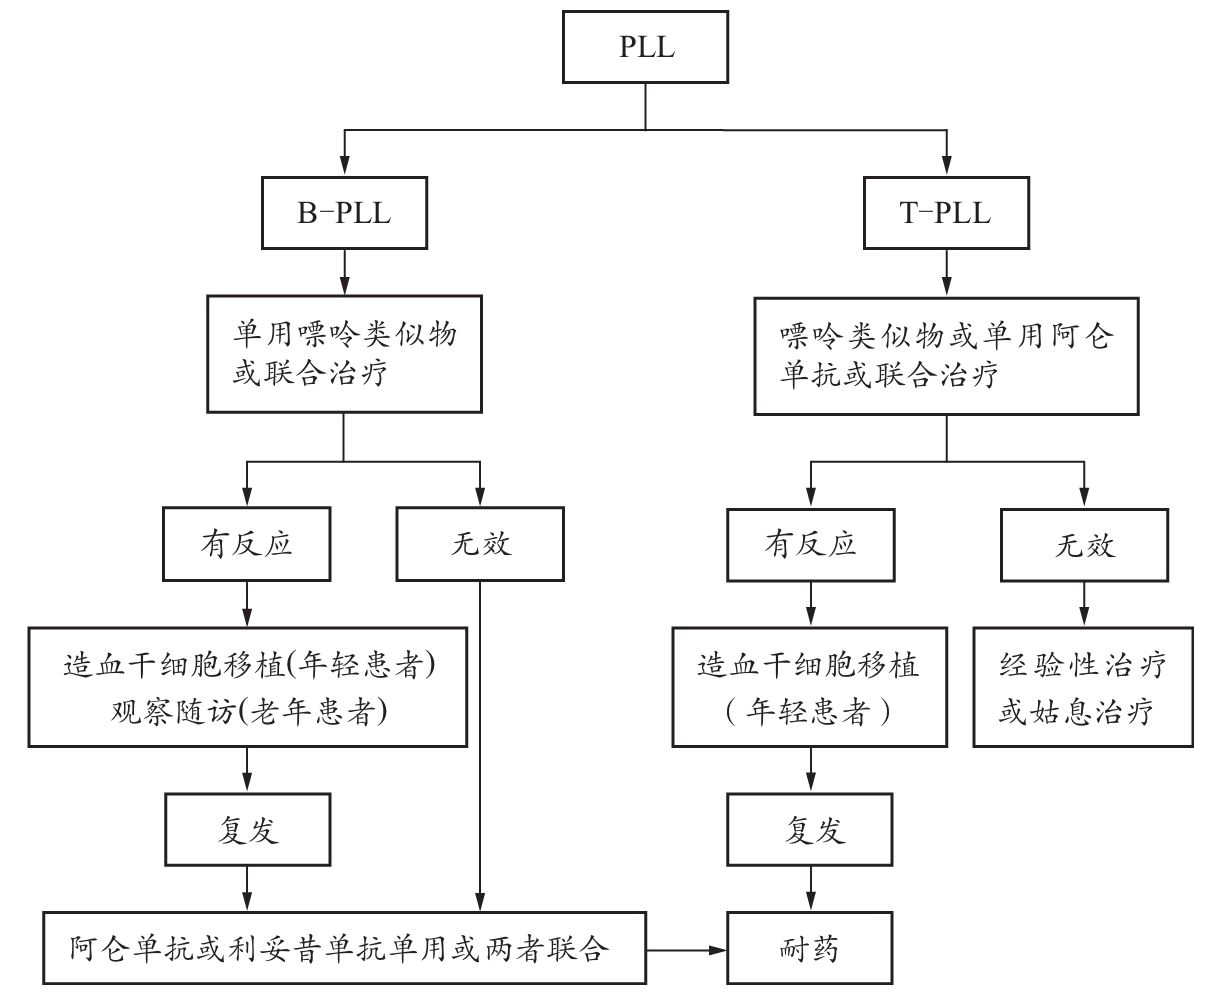
\includegraphics{./images/Image00147.jpg}
 \captionsetup{justification=centering}
 \caption{幼淋巴细胞白血病的治疗程序}
 \label{fig5-1-14}
  \end{figure} 

【治疗方案】

1. 支持治疗 详见急性白血病章节。

2. 化疗

(1)B-PLL的治疗方案:

1)CHOP方案:

\begin{longtable}[]{@{}ll@{}}
\toprule
\endhead
\vtop{\hbox{\strut 环磷酰胺 750mg/m$^2$}\hbox{\strut NS 100ml}} &
静脉滴注,每日1次,d1\tabularnewline
\bottomrule
\end{longtable}

\begin{longtable}[]{@{}ll@{}}
\toprule
\endhead
\vtop{\hbox{\strut 多柔吡星 50mg/m$^2$}\hbox{\strut 5\% GS 250ml}} &
静脉滴注,每日1次,d1\tabularnewline
\bottomrule
\end{longtable}

\begin{longtable}[]{@{}ll@{}}
\toprule
\endhead
\vtop{\hbox{\strut 长春新碱 1.4mg/m$^2$
(最大每日剂量2mg)}\hbox{\strut NS 20ml}} &
静脉注射,每日1次,d1\tabularnewline
\bottomrule
\end{longtable}

泼尼松 60mg/(m$^2$ ·d),口服,d1~d5

21日1疗程

2)单药氟达拉滨:

\begin{longtable}[]{@{}ll@{}}
\toprule
\endhead
\vtop{\hbox{\strut 氟达拉滨 25mg/(m$^2$ ·d)}\hbox{\strut NS 100ml}} &
静脉滴注,每日1次,d1~d5\tabularnewline
\bottomrule
\end{longtable}

28日1疗程

3)单药喷司他丁:

\begin{longtable}[]{@{}ll@{}}
\toprule
\endhead
\vtop{\hbox{\strut 喷司他丁 4mg/m$^2$}\hbox{\strut NS 500ml}} &
静脉滴注,每周1次×3,然后每2周1次×3,其后有反应者1个月1次,最多不超过6个月\tabularnewline
\bottomrule
\end{longtable}

4)单药克拉屈滨:

\begin{longtable}[]{@{}ll@{}}
\toprule
\endhead
\vtop{\hbox{\strut 克拉屈滨 0.1mg/(kg·d)}\hbox{\strut NS 500ml}} &
静脉滴注(连续滴注),每日1次,d1~d7\tabularnewline
\bottomrule
\end{longtable}

\begin{longtable}[]{@{}ll@{}}
\toprule
\endhead
\vtop{\hbox{\strut (或)克拉屈滨 0.14mg/(kg·d)}\hbox{\strut NS 500ml}}
&
静脉滴注(连续滴注超过2小时),每日1次,d1~d5\tabularnewline
\bottomrule
\end{longtable}

28日1疗程

5)FC方案:

\begin{longtable}[]{@{}ll@{}}
\toprule
\endhead
\vtop{\hbox{\strut 氟达拉滨 25mg/(m$^2$ ·d)}\hbox{\strut NS 100ml}} &
静脉滴注,每日1次,d1~d3\tabularnewline
\bottomrule
\end{longtable}

\begin{longtable}[]{@{}ll@{}}
\toprule
\endhead
\vtop{\hbox{\strut 环磷酰胺 250mg/(m$^2$ ·d)}\hbox{\strut NS 100ml}}
& 静脉滴注,每日1次,d1~d3\tabularnewline
\bottomrule
\end{longtable}

28日1疗程

6)FCM方案:

\begin{longtable}[]{@{}ll@{}}
\toprule
\endhead
\vtop{\hbox{\strut 氟达拉滨 25mg/(m$^2$ ·d)}\hbox{\strut NS 100ml}} &
静脉滴注,每日1次,d1~d3\tabularnewline
\bottomrule
\end{longtable}

\begin{longtable}[]{@{}ll@{}}
\toprule
\endhead
\vtop{\hbox{\strut 环磷酰胺 200mg/(m$^2$ ·d)}\hbox{\strut NS 100ml}}
& 静脉滴注,每日1次,d1~d3\tabularnewline
\bottomrule
\end{longtable}

\begin{longtable}[]{@{}ll@{}}
\toprule
\endhead
\vtop{\hbox{\strut 米托蒽醌 8mg/m$^2$}\hbox{\strut NS 100ml}} &
静脉滴注,每日1次,d1\tabularnewline
\bottomrule
\end{longtable}

28日1疗程

7)FC±利妥昔单抗方案:

\begin{longtable}[]{@{}ll@{}}
\toprule
\endhead
\vtop{\hbox{\strut 氟达拉滨 25mg/(m$^2$ ·d)}\hbox{\strut NS100ml}} &
静脉滴注,每日1次,d1~d3\tabularnewline
\bottomrule
\end{longtable}

\begin{longtable}[]{@{}ll@{}}
\toprule
\endhead
\vtop{\hbox{\strut 环磷酰胺 250mg/(m$^2$ ·d)}\hbox{\strut NS 100ml}}
& 静脉滴注,每日1次,d1~d3\tabularnewline
\bottomrule
\end{longtable}

\begin{longtable}[]{@{}ll@{}}
\toprule
\endhead
\vtop{\hbox{\strut 利妥昔单抗 375mg/m$^2$}\hbox{\strut NS 500ml}} &
静脉滴注,每日1次,d0\tabularnewline
\bottomrule
\end{longtable}

28日1疗程

8)阿仑单抗+利妥昔单抗方案:用于复发/难治、遗传学检查具有17p-的患者

\begin{longtable}[]{@{}ll@{}}
\toprule
\endhead
\vtop{\hbox{\strut 阿仑单抗*}\hbox{\strut NS 500ml}} &
静脉滴注(2小时滴完)\tabularnewline
\bottomrule
\end{longtable}

*:阿仑单抗 3mg,d1,10mg,d3和30mg,d5,以后30mg,每周2次至12周

\begin{longtable}[]{@{}ll@{}}
\toprule
\endhead
\vtop{\hbox{\strut 利妥昔单抗 375mg/m$^2$}\hbox{\strut NS 500ml}} &
静脉滴注,d1,d8,d15,d22,每日1次\tabularnewline
\bottomrule
\end{longtable}

(2)T-PLL的治疗方案:

1)单药阿仑单抗:

\begin{longtable}[]{@{}ll@{}}
\toprule
\endhead
\vtop{\hbox{\strut 阿仑单抗*}\hbox{\strut NS 500ml}} &
静脉滴注(连续2小时滴注)\tabularnewline
\bottomrule
\end{longtable}

*:阿仑单抗 3mg,d1,10mg,d3和30mg,d5,以后30mg,每周3次至12周

2)单药喷司他丁:

\begin{longtable}[]{@{}ll@{}}
\toprule
\endhead
\vtop{\hbox{\strut 喷司他丁 4mg/m$^2$}\hbox{\strut NS 500ml}} &
静脉滴注,每周1次,连续4周,然后每隔两周1次,直至获得最大反应\tabularnewline
\bottomrule
\end{longtable}

【疗效观察与随访】

1. 观察指标

(1)症状、体征:观察发热、盗汗等B组症状的变化,浅表淋巴结、脾脏等大小的变化。

(2)血常规、骨髓、CT:根据白细胞、红细胞、血小板及骨髓幼稚淋巴细胞数等改变综合疗效。

2. 疗效评估 临床缓解:症状、体征改善,血象、骨髓象进步,但总体预后差。

3.
随访 注意观察病情,观察症状体征的变化,注意饮食起居,避免感冒,避免并发症。定期复查血象、骨髓象。

【治疗经验与解析】

1.
PLL需与CLL/PL、套细胞淋巴瘤[具有特征性的t(11;14)]、脾边缘区淋巴瘤、多毛细胞白血病变异型等鉴别。

2.
使用利妥昔单抗前30分钟,静脉注射地塞米松5mg、肌内注射非那根25mg预防过敏。第1次使用的第1个100mg应静脉滴注维持4小时,以后开始速度为50mg/h,如无不良反应,每30分钟递增50mg/h,最大可达400mg/h,同时给予床边心电监测。治疗过程中若发生低血压或支气管痉挛时,应暂时停止滴注,并给予抗过敏药,必要时给予支气管扩张药,症状均可减轻。由于在药物输入过程中可能发生暂时性低血压,所以在输入本药前12小时及输入过程中停止抗高血压药治疗。

3.
使用阿仑单抗前30分钟予以苯海拉明50mg和对乙酰氨基酚650mg预防和减轻输液反应。如果出现严重输液反应,予以氢化可的松200mg;用药前予以磺胺类药物和泛昔洛韦及类似药物预防感染,直至停药后2个月或者CD4+细胞达到2×10$^{8}$
/L以上;治疗期间每1~2周监测巨细胞病毒抗原;如果停药时间超过7日,则从3mg起用,渐渐加量至10mg或30mg。

\paragraph{大颗粒淋巴细胞白血病}

大颗粒淋巴细胞(LGL)白血病在1985年首次被描述为有关血液、骨髓及脾脏的克隆性疾病。1993年Sokolet等将LGL分为T、NK细胞系,并被所有病理分型系统采纳。LGL克隆性疾病是一组异质性较大的淋巴样恶性疾病,T细胞及NK细胞型在临床上均可表现为惰性或进展型。WHO对淋巴系统恶性肿瘤的分类中包括T-LGL白血病及侵袭性NK细胞白血病,上述两种疾病均可作为T/NK细胞淋巴瘤/白血病中单一亚型。T-LGL白血病是西方国家中最常见的LGL异常,约占LGL白血病总病例数的85\%,大多数临床过程呈惰性,生存期长达10年以上,中位诊断年龄为60岁,无性别差异。侵袭性NK细胞白血病预后差,约占所有LGL疾病的10\%,多见于亚洲人群,好发于青壮年,中位发病年龄为39岁,男女比例相似,有证据表明其发病与EB病毒感染高度相关。

【治疗程序】 如图\ref{fig5-1-15}所示。

\begin{figure}[!htbp]
 \centering
 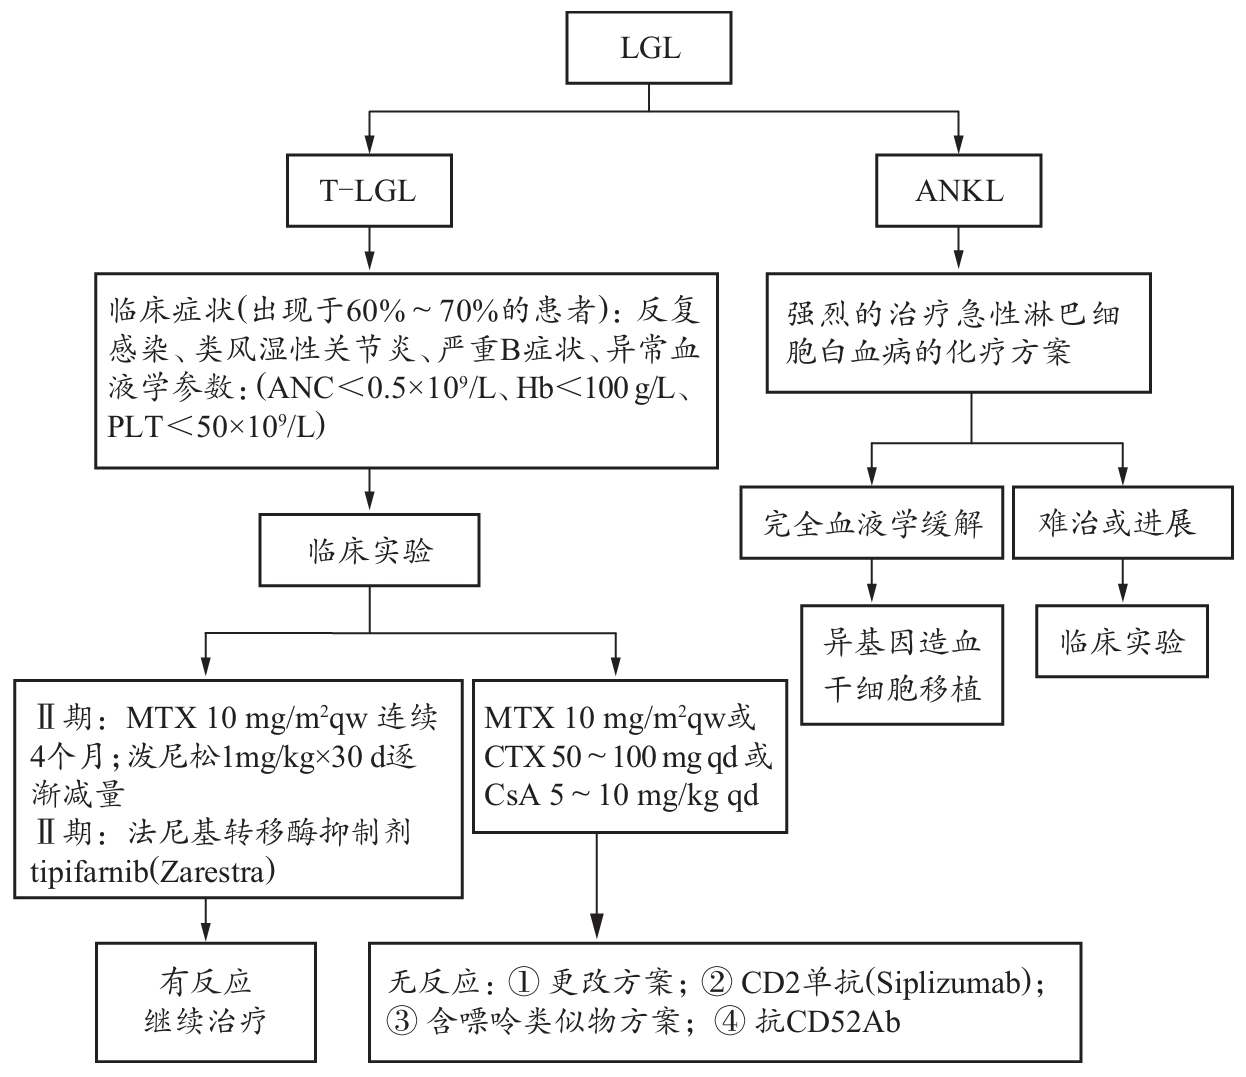
\includegraphics{./images/Image00148.jpg}
 \captionsetup{justification=centering}
 \caption{大颗粒淋巴细胞白血病的治疗程序}
 \label{fig5-1-15}
  \end{figure} 

【治疗方案】

1.
支持治疗 对于伴有严重粒缺及同时使用激素治疗的患者,有必要预防性使用抗生素。全血细胞减少时,针对病情选择输注红细胞或血小板支持,造血生长因子,尤其是促红细胞生成素,粒细胞集落刺激因子等也有一定疗效。累及脏器功能时,积极对症、支持治疗,保护脏器功能。

2. 药物治疗

(1)T-LGL治疗方案:

1)免疫抑制治疗:甲氨蝶呤能有效诱导反应,单一使用MTX治疗的有效率近50\%。然而,患者可能需要进一步的治疗以维持疗效,如MTX,10mg/m$^2$
,每周1次。环磷酰胺(CTX,50~100mg/d)或环孢素A[CsA,5~10mg/(kg·d)]也是有效治疗。目前认为这些药物起效主要是通过免疫调节机制,而并非对T细胞LGL的细胞毒作用。

2)糖皮质激素:糖皮质激素也有一定的疗效,在治疗的第1个月,联合CTX或MTX可能更快的改善B症状及获得血液学的改善。但因为其副作用,不建议长程(\textgreater{}1个月)使用大剂量的糖皮质激素,如泼尼松1mg/kg口服,每日1次,连续30日后缓慢减量。

3)嘌呤类似物:氟达拉滨、克拉曲滨、喷司他丁等嘌呤类似物为基础的方案亦有相当疗效,清除恶性克隆优于MTX、CsA等,如FND方案:

\begin{longtable}[]{@{}ll@{}}
\toprule
\endhead
\vtop{\hbox{\strut 氟达拉滨 25mg/(m$^2$ ·d)}\hbox{\strut NS 100ml}} &
静脉滴注,每日1次,d1~3\tabularnewline
\bottomrule
\end{longtable}

\begin{longtable}[]{@{}ll@{}}
\toprule
\endhead
\vtop{\hbox{\strut 米托蒽醌 10mg/m$^2$}\hbox{\strut NS 100ml}} &
静脉滴注20分钟,避光,d1\tabularnewline
\bottomrule
\end{longtable}

地塞米松 20mg/d,口服,d1~5 28日1疗程

4)阿仑单抗:T-LGL白血病细胞表达CD52,阿仑单抗可应用于难治的T-LGL白血病患者,如阿仑单10mg,静脉滴注(维持2小时滴注),每日1次,连续10日。

(2)ANKL治疗方案:侵袭性NK细胞白血病具体方案参见急性淋巴细胞白血病化疗。

【疗效观察与随访】

1. 观察指标 血象,出凝血相关指标、骨髓常规、尿常规。

2. 缓解标准 症状、体征减轻,相关检测指标改善,病情稳定3个月以上。

3.
随访 主要观察贫血、出血等相关症状和体征,定期检测血常规、生化、骨髓常规等。注意饮食起居,避免感冒,避免并发症。

【治疗经验与解析】

1.
LGL白血病临床表现异质性较大,有些患者淋巴细胞绝对值并无升高,某些患者的白血病细胞并没有粗大颗粒,此时诊断较为困难,主要依靠免疫表型与TCR基因克隆性重排诊断。

2.
T-LGL白血病中侵袭性亚型病例数极少,此亚型未出现在WHO分类中。一过性的(<6个月)及慢性的(\textgreater{}6个月)LGL增多是LGL异常中的两种良性状态。一过性反应性的LGL增多可出现在病毒感染、免疫异常、恶性肿瘤及部分进行实体器官移植后的患者。反应性的LGL是多克隆的,在大多数病例表达T细胞免疫表型(CD3+),LGL计数自行恢复正常或治疗后正常,通常在6个月之内。

3.
在T-LGL白血病患者,有25\%~50\%伴有免疫异常,T-LGL常并发类风湿关节炎,纯红再障或周期性中性粒细胞减少。而CMV或HIV感染可导致反应性或一过性LGL升高,在鉴别诊断时予以区分。

4. T-LGL白血病治疗一般需持续至少4个月,若无效,则再改用其他治疗方案。

5.
由于缺乏克隆标记,NK细胞克隆性很难确定,因此不能确定是慢性NK细胞增多,还是慢性NK细胞白血病,因而临床表现是鉴别诊断这两种情况的最重要的依据。有系统性症状或有肝、脾、骨髓浸润的患者一般归类于慢性NK细胞白血病。无症状的患者倾向于归类至良性慢性NK细胞增多。

\paragraph{肥大细胞白血病}

肥大细胞白血病(MCL)又称组织嗜碱细胞白血病,是一种由肥大细胞恶性增生,引起各种器官如肝、脾、皮肤和血液及淋巴造血系统等一系列病理学改变的疾病。原发性者少见,多继发于系统性肥大细胞增多症(SM)。MCL是一种极为少见的白血病,约占恶性肥大细胞肿瘤的15\%,国内仅有个案报道。其病因未明,有报告称发病可能和C-KIT基因突变有关。

【治疗程序】 如图\ref{fig5-1-16}所示。

\begin{figure}[!htbp]
 \centering
 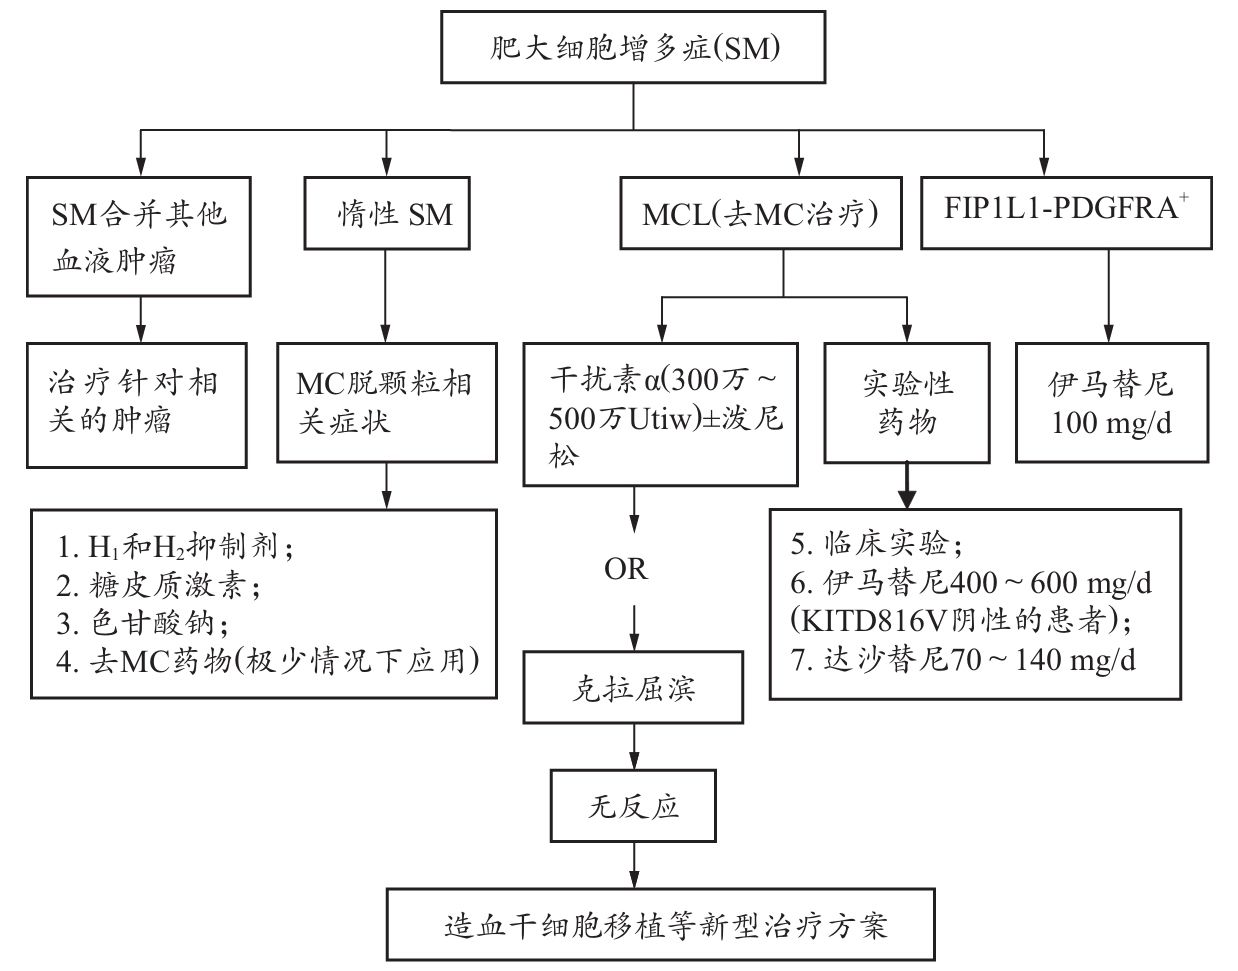
\includegraphics{./images/Image00149.jpg}
 \captionsetup{justification=centering}
 \caption{肥大细胞白血病的治疗程序}
 \label{fig5-1-16}
  \end{figure} 

【治疗方案】 目前尚无有效的治疗方法。糖皮质激素、烷化剂、抗组胺药物仅适用于早期患者。MCL患者也可采用含有干扰素、伊马替尼或克拉屈滨的治疗,对于少数进展迅速、恶性程度较高的MCL可以考虑进行异基因造血干细胞移植。具体的药物用法为:

1. 抗组胺H{1}
受体药物 主要用于控制皮肤相关症状。酮替芬1mg,口服,每日2次,或西替利嗪10mg,口服,每日1次。

2. 抗组胺H{2}
受体药物 主要控制胃肠道反应相关的症状。雷尼替丁150mg,口服,每日2次。

3. 糖皮质激素 泼尼松0.2~2mg/kg,口服,每日1次。

4.
色甘酸钠 主要用于胃肠道反应相关的症状。色甘酸钠100~600mg,口服,每日3次。

5. 干扰素α 300万~500万U,皮下注射,每周3次。

6. 单药克拉屈滨 5mg/(m$^2$
·d),静脉滴注(连续滴注),连续5日,28日1疗程。

7.
酪氨酸激酶抑制剂 伊马替尼400~600mg/d,口服,每日1次,或达沙替尼70~140mg/d,口服,每日1次。

【疗效观察与随访】

1. 观察指标 血常规、骨髓常规、肝脾B超检查等。

2. 缓解标准 症状、体征改善,相关检测指标改善,病情稳定3个月以上。

3.
随访 主要观察症状和体征等变化,可定期复查血常规、生化等检查;定期复查外周血骨髓中肥大细胞的比例。

【治疗经验与解析】 伊马替尼、达沙替尼主要副作用为血液学毒性,应注意血液学监测和支持治疗。常见非血液学毒性包括水肿、恶心、腹泻、皮疹、骨关节痛、肌痉挛和肝酶异常等。伊马替尼治疗失败主要由耐药导致,存在KITD816V基因突变的患者对其无效,因此治疗前需行该基因检测。

\subsection{骨髓增生异常综合征}

骨髓增生异常综合征(MDS)是一种起源于造血干细胞的恶性克隆性疾病,其临床特征主要是造血细胞一系或多系发育异常、无效造血所致的难治性血细胞减少和高风险转化为急性髓系白血病。MDS多见于老年人,年发病率在3~5/10万。MDS可分为原发性MDS和继发性MDS,后者与长期接触苯,或因某些肿瘤而接受放疗、化疗相关。

【治疗程序】 如图\ref{fig5-1-17}所示。

\begin{figure}[!htbp]
 \centering
 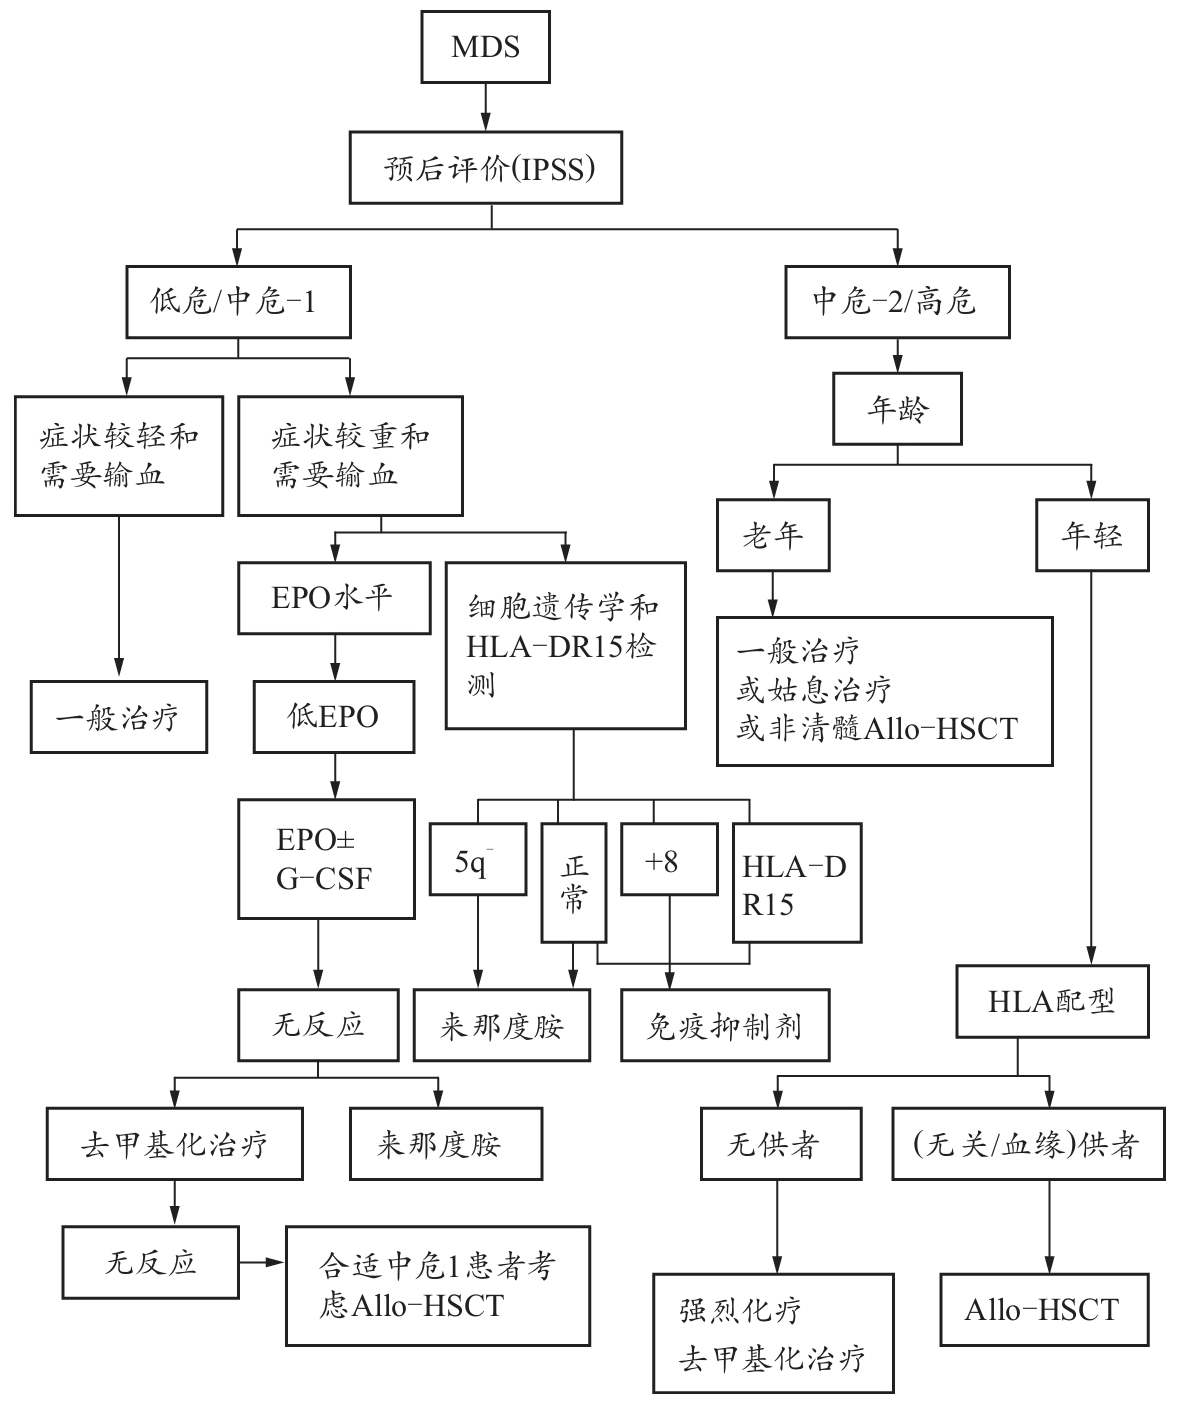
\includegraphics{./images/Image00150.jpg}
 \captionsetup{justification=centering}
 \caption{骨髓增生异常综合征的治疗程序}
 \label{fig5-1-17}
  \end{figure} 

【治疗方案】 治疗是以国际预后积分系统(IPSS)危度分组为依据,对于低危和中危-1患者,主要是刺激残存造血干、祖细胞的造血能力和(或)改善MDS异常造血克隆的造血效率,从而改善患者的生活质量,对于中危-2和高危患者,则是根除MDS异常造血克隆恢复正常造血。

1.
一般治疗 避免接触可能的致病因素。临床症状不明显者可仅观察随访。对重度贫血而有自觉症状者可输注红细胞悬液;对有明确感染者,应给予有效的抗生素治疗;血小板数严重减少伴有明显的出血者可输血小板,维持血小板\textgreater{}10×10$^{9}$
/L。对于长期红细胞输注\textgreater{}20~30U或血清铁蛋白\textgreater{}2500μg/L,且预计生存期较长(以年计)者,常用去铁胺去铁治疗,直至<1000μg/L,去铁胺20~40mg/(kg·d),微量泵皮下持续注射12小时,每周5~7日。

2. 姑息或对症治疗 姑息治疗包括生物反应调节剂或低剂量化疗。

(1)针对其全血细胞减少,可选用:

EPO 10000U,皮下注射,每日1次

G-CSF或GM-CSF 150~300μg,皮下注射,每日1次

IL-11 10μg/kg,皮下注射,每日1次

血小板生成素(TPO) 10000U,皮下注射,每日1次

(2)免疫抑制治疗应用于某些MDS亚型,特别是伴严重血细胞减少的低增生性MDS。如:

CsA 2~6mg/(kg·d),口服,每日2次

血液CSA浓度维持100~300ng/ml

兔ATG 3~5mg/(kg·d),加入NS1000ml中,静脉滴注,维持12~16小时,连用5日

(3)小剂量化疗,常用小剂量药物治疗,如:

阿糖胞苷 10~20mg/d,皮下注射,2周为1个疗程,间歇2周后重复使用

高三尖杉酯碱 0.5~1mg/d,静脉滴注,2周为1个疗程,间歇2周后再开始下一个疗程

阿克拉霉素 5mg/(m$^2$ ·d),静脉滴注,7日为1个疗程,一般用2个疗程。

或联合化疗方案如CAG、HAG。

3.
高强度治疗 包括异基因造血干细胞移植(Allo-HSCT)和强烈诱导化疗如标准或大剂量Ara-C联合蒽环类或氟达拉滨方案,具体参照AML相关章节。

4.
DNA甲基转移酶抑制剂 适用于中危-2及高危患者,特别是老年不适合强烈化疗及HSCT的患者。常用有5氮杂胞苷75mg/(m$^2$
·d),皮下注射,d1~7,4周为1个疗程,至少4疗程;地西他滨20mg/m$^2$
加入250ml生理盐水,静脉滴注,d1~5,4周为1个疗程,至少3个疗程。

5. 免疫调节剂 适用于伴5q{-}
伴/不伴额外细胞遗传学异常且有输血依赖的低、中危患者。如沙利度胺100~200mg,口服,每日2次;来那度胺10mg口服,每日1次。

【疗效观察与随访】

1. 观察指标

(1)症状:观察患者是否有进行性加重的贫血、出血倾向及反复发生的感染等。

(2)血常规:全血细胞减少进行性加重,提示病情进展,预后差。

(3)染色体:出现新的染色体异常,提示病情进展,预后差。

(4)骨髓:原始细胞增高,当\textgreater{}20\%,提示转化为急性髓系白血病。

2.
疗效标准 关于骨髓增生异常综合征的疗效标准,在很长时间内没有国际统一认同的标准。为解决这一问题,2000年Cheson等专家组提出了统一的标化疗效标准。具体见表\ref{tab5-1-4}。

表\ref{tab5-1-4} 标化MDS疗效判定标准*

\begin{longtable}[]{@{}l@{}}
\toprule
\endhead
完全缓解(CR)\tabularnewline
1. 骨髓(BM):反复骨髓穿刺示原始细胞<5\%{\#}
,各系细胞成熟正常,无发育异常的形态表现{Δ}\tabularnewline
\vtop{\hbox{\strut 2.
外周血(PB):绝对值必须在不要造血生长因子的情况下维持2个月:}\hbox{\strut (1)血红蛋白(Hb)\textgreater{}110g/L}\hbox{\strut (2)中性粒细胞≥1.5×10$^{9}$
/L}\hbox{\strut (3)血小板(BPC)≥100×10$^{9}$
/L}\hbox{\strut (4)无原始细胞}\hbox{\strut (5)血细胞无发育异常表现}}\tabularnewline
部分缓解(PR)\tabularnewline
1.
BM原始细胞较前减少50\%或更多;或与之前FAB亚型相比转变为较轻的亚型(不管有核细胞增生程度和发育异常表现)\tabularnewline
2. PB绝对值需至少维持2个月\tabularnewline
3. 其余同CR标准\tabularnewline
4. 血液学改善(HI){▲}
:改善值必须在不用细胞毒药物治疗的情况下,至少维持2个月:\tabularnewline
\vtop{\hbox{\strut (1)红细胞和血红蛋白(HI-E)}\hbox{\strut 显效:治疗前Hb<110g/L,治疗后升高20g/L以上;治疗前依赖输血者,治疗后脱离输血}\hbox{\strut 有效:治疗前Hb<110g/L,治疗后升高10~20g/L;治疗前依赖输血者,治疗后需求减少50\%}}\tabularnewline
\vtop{\hbox{\strut (2)血小板(HI-P)}\hbox{\strut 显效:治疗前BPC<100×10$^{9}$
/L,治疗后升高30×10$^{9}$
/L,或更多治疗前依赖输BPC者,脱离输BPC,BPC数维持稳定}\hbox{\strut 有效:治疗前BPC<100×10$^{9}$
/L,治疗后升高50\%或更多;净增值\textgreater{}10×10$^{9}$
/L,但<30×10$^{9}$ /L}}\tabularnewline
\vtop{\hbox{\strut (3)中性粒细胞(HI-N)}\hbox{\strut 显效:治疗前中性粒细胞绝对计数(ANC)<1.5×10$^{9}$
/L,治疗后增加100\%或净增数≥0.5×10$^{9}$
/L}\hbox{\strut 有效:治疗前ANC<1.5×10$^{9}$
/L,治疗后只是增加100\%,但净增数<0.5×10$^{9}$
/L}}\tabularnewline
\bottomrule
\end{longtable}

注:*:所有疗效标准必须是根据治疗后适当日期(≥1个月)相隔至少1周的至少连续2次测定值加以判定。\#:如红系\%<有核细胞(NC)的50\%,原始细胞\%按NC\%计算;如红系\%≥有核细胞(NC)的50\%,原始细胞\%按非红系细胞(NEC)计算。Δ:如考虑为治疗影响所致,可允许有轻度巨幼样变,但不能有治疗前存在的其他形态异常。▲:按有效的血细胞系列报告。

3.
随访 注意病情观察,观察症状、血常规、染色体、骨髓等变化,避免并发症。

【治疗经验与解析】

1.
MDS患者治疗的初次策略须考虑以下4点:①IPSS危险度,②年龄,③体能状态,④输血的依赖程度。在治疗过程中应对患者病情动态评估以调整治疗策略。

2.
关于预后积分系统(IPSS),IPSS是目前血液科医生广泛接受的预后判断系统,但该系统呈静止状态,没有融入患者年龄、病情进展速度及输血依赖情况等重要因素。而目前研究证实在MDS患者的病程中是否输血能极大影响患者的预后并有可能成为评价疾病严重程度的独立因素。如何动态的分层评估患者的预后对于调整和确定治疗方案有较大的意义。

3.
关于异基因造血干细胞移植(Allo-HSCT) Allo-HSCT是目前唯一能根治MDS的措施,患者年龄、疾病状态和供者来源是影响患者移植后长期生存率的重要因素。目前行Allo-HSCT的指征包括:①年龄<55岁的中危2或高危患者如能找到HLA匹配的同胞供体,应在确诊后立即施行Allo-HSCT。②年龄<40岁的中危-1、中危-2或高危患者可以施行HLA匹配的无关供体Allo-HSCT。③低危或中危-1患者如选择HSCT,则应在出现新的染色体异常、进行性加重的血细胞减少以及进展为更高IPSS危险度时施行。我国的专家共识认为:<60岁,中危-2、高危组和具有明确恶性克隆证据或血小板长期<20×10$^{9}$
/L或严重依赖于输血的中危-1患者,应首选HLA相合的HSCT;对于无HLA相合的高危患者,可以选择单倍体相合HSCT。

\section{红细胞疾病}

\subsection{缺铁性贫血}

缺铁性贫血(IDA)是由于体内铁缺乏影响血红蛋白合成所引起的一种小细胞低色素性贫血。这种贫血的特点是骨髓、肝、脾及其他组织中缺乏可染色铁,血清铁蛋白、血清铁浓度和血清转铁蛋白饱和度均降低,发病率甚高。男性发病率约10\%,女性发病率大于20\%,其中孕妇占60\%~80\%。IDA的主要原因包括:①铁需要量增加而摄入不足;②铁吸收不良;③铁丢失过多如慢性失血等,上述原因均会影响血红蛋白和红细胞生成而发生贫血。缺铁发生的主要危险因素在青少年为营养因素,月经期妇女为月经过多,中老年缺铁性贫血患者则应警惕消化道肿瘤的存在。IDA分期分为缺铁期(贮存铁缺乏期),缺铁性红细胞生成期,缺铁性贫血期。

【治疗方案】 治疗原则:①病因治疗:尽可能除去引起缺铁和贫血的原因。②补充足够量的铁以供机体合成血红蛋白,补充体内铁的贮存量至正常水平。

1.
病因治疗 IDA患者必须要明确病因,病因治疗对纠正贫血的效果、速度及防止其复发均有重要意义。确诊为IDA后要详细询问病史,了解是否有肠道、肛门、阴道慢性失血情况,了解饮食习惯。若发现肠道畸形、肿瘤、钩虫病等慢性失血,在纠正贫血的同时应行外科手术和驱虫治疗。长期月经增多要请妇科协助处理。

2. 铁剂治疗

(1)口服铁剂:硫酸亚铁控释片(福乃得500mg,qd),于每晨饭后服。第二代可溶性铁剂:小分子有机酸铁盐络合物,如富马酸铁0.2g,tid;琥珀酸亚铁(速力菲)0.1g,tid,含铁量较高,起效较快;多糖铁复合物(力蜚能0.15g,bid),胃肠道反应很小,适用于孕妇口服补铁。

(2)注射铁剂:

1)右旋糖酐铁:首次给药0.5ml(约10mg)深部肌内注射,观察1小时无过敏反应,可继续治疗,第1日剂量50mg;然后100mg隔日或每周2~3次,直至完成治疗总剂量。铁剂总量=体重(kg)×[150-患者Hb(g/L)]×0.24+500mg。

2)蔗糖铁注射液:适用于诊断明确、口服铁剂不能耐受或吸收不好的患者。用药前根据公式以此确定每个患者的给药量:

总缺铁量(mg)=[正常Hb-患者Hb(g/L)]×体重(kg)×0.24+贮存铁(mg)

需与0.9\%生理盐水混合,以滴注或缓慢注射的方式静脉给药。根据血红蛋白水平每周用药2~3次,剂量为成年人和老年人每次5~10ml(100~200mg铁),儿童为每次0.15ml/kg。给药频率应不超过每周3次。第1次治疗前成人用1~2.5ml进行测试,如果在给药15分钟后未出现任何不良反应,继续给予余下的药液。静脉蔗糖铁不含右旋糖酐,极少发生过敏反应。并且几乎完全通过网状内皮系统摄取,不沉积在肝内,从而避免了肝损伤。

【疗效观察与随访】

1.
观察指标 血常规、网织红细胞、血清铁、血清铁饱和度、血清铁蛋白、总铁结合力,并计算MCI、MCH、MCHC等。

2.
治愈标准 病因消除,贫血纠正,相关检测指标恢复正常,半年内未复发。3.随访 通过动态检测血常规和网织红细胞评估治疗效果。一般口服铁剂

有效者在服药3~4日后,网织红细胞开始上升,7~10日可达到15\%~16\%,半月后逐渐下降,此为网织红细胞反应。血红蛋白和红细胞服药一周后开始上升,平均每日可上升15~20g/L,2周后血红蛋白较治疗前增加20~30g/L可做为铁剂治疗的有效指征。血红蛋白恢复正常后,仍需继续服用铁剂3~6个月,或直至血清铁蛋白恢复到50μg/ml,以补足贮备铁。连服铁剂2~3周无效者,应查明原因,采取相应措施。

【治疗经验与解析】

1.
通过实验室检查诊断IDA较简单,但病因诊断较IDA本身更加重要,中老年人饮食正常情况下缺铁需要反复检查粪便隐血以免漏诊肠道恶性肿瘤;女性阴道出血量增加可能是妇科疾患的信号,需要妇科医生详细检查并进行病因治疗。

2.
口服铁剂需在饭后1小时服用,每日3~4次。服药时忌茶,以免铁被鞣酸沉淀而不能被吸收;由于牛奶中含有较多的磷酸盐,影响铁剂吸收,不宜同服;碱性药物(碳酸氢钠、胃舒平等)可影响铁的吸收;同时加服维生素C和微量元素可加强铁剂的吸收。

3.
注射铁剂可引起局部疼痛、荨麻疹、发热、头痛、关节疼痛、恶心、哮喘等,严重过敏性休克需慎用。注射铁剂的总需量按公式计算。常见副作用有头痛、发热、荨麻疹。

4.
仅在下列情况下才考虑应用注射铁剂:①口服铁剂不能吸收,例如胃切除或胃肠吻合术后、慢性腹泻、脂肪痢等;②对口服铁剂有严重的胃肠道反应,例如消化性溃疡,溃疡性结肠炎、节段性结肠炎、胃切除后胃肠功能紊乱及妊娠时持续呕吐等;③慢性失血(铁)过多,口服铁剂不足以补充;④原患严重胃肠道疾病,口服铁剂可能使病情加重,如溃疡性结肠炎;⑤怀孕晚期伴严重IDA,急需治疗。

5.
对贫血症状严重、Hb<60g/L的患者或有合并症者,可输注浓缩红细胞或添加液红细胞。

\subsection{铁粒幼细胞性贫血}

铁粒幼细胞性贫血(SA)是一组铁利用障碍性疾病。特征为骨髓中出现大量环状铁粒幼红细胞,红细胞无效生成,组织铁储量过多和小细胞低色素性贫血。本病分为遗传性和获得性,还有维生素B{6}
反应性贫血。遗传性SA包括X连锁(XLSA)、常染色体隐性遗传和与线粒体DNA突变相关的SA;获得性SA分为原发性和继发于药物、毒物、慢性肿瘤性和炎症性疾病相关SA。

【治疗方案】

1.
一般治疗 对于药物、慢性乙醇中毒、铅中毒引起的,停药或戒酒后,贫血可恢复;慢性病所致者以治疗原发病为主。

2. 药物治疗

(1)维生素B{6}
(吡哆醇):采用大剂量治疗小剂量维持的方法。1/3的XLSA患者对吡哆醇有效,剂量为75~150mg,qd,至少3个月。吡哆醇生效可使血液中稳态血红蛋白增加,减少输血,停用吡哆醇后,贫血又会复发,再用吡哆醇治疗仍有效,但疗效不如第1次。建议吡哆醇大剂量治疗后有效者以37.5~75mg,qd维持。

(2)去铁治疗:

1)静脉放血:如血红蛋白无明显下降可每2周放血1次,每次250~350ml或(4~5)ml/kg。

2)注射用甲磺酸去铁胺(得斯芬):是临床上常用的铁螯合剂,建议在最初的10~20次输血后或血清铁蛋白水平已达到1000ng/ml时开始用本品进行治疗。剂量的安排和给药方式都应个体化,治疗过程中根据其铁负荷的严重程度而进行调整。应使用最小有效剂量。平均日剂量通常在20~60mg/kg。血清铁蛋白水平低于2000ng/ml的患者每日需用量大约在25mg/kg。血清铁蛋白水平在(2000~3000)ng/ml之间每日需用量约35mg/kg。血清铁蛋白浓度较高的患者,最大剂量可能达到55mg/(kg·d)。铁负荷过载患者通常会有维生素C缺乏,可能是由于铁氧化了维生素。维生素C可用作螯合治疗的辅助治疗。最大剂量为每日200mg,分次服用,并在用本品进行正规治疗1个月以后开始服用。甲磺酸去铁胺首选的用药方法是持续静脉滴注。推荐的最大滴注速度是15mg/(kg·h)。通常在用药4~6小时之后,条件允许时应减慢滴速,使之24小时总的静脉用药量不超过推荐剂量80mg/kg。

得斯芬试验:肌内注射本品500mg,然后收集6小时尿液送验铁含量。如6小时尿铁含量为1~1.5mg(18~27μmol)表示有铁负荷过载。超过1.5mg(27μmol)者可认为是病理性的。此试验只有在肾功能正常的病例,才能得到可靠的结果。应使用本品的10\%水溶液用于注射。5ml注射用水注入含有500mg本品的小瓶中,充分摇动。只能使用清亮溶液。

【疗效观察与随访】

1.
观察指标 血常规、血红蛋白电泳分析、骨髓常规、铁染色分析、得斯芬试验等。

2. 好转标准 症状改善,相关检测指标未能完全恢复正常。

3. 随访 密切观察病情变化,定期复查相关指标,注意治疗效果。

对吡哆醇治疗有效者能生存多年,无效者常因血色病并发症导致心功能衰竭、肝衰竭或继发感染而死亡。经吡哆醇治疗后患者可达完全或部分缓解,血红蛋白增加,血清铁减低,但红细胞形态异常不能完全消失(MCV,MCH和RDW),异常的铁粒幼细胞仍存在。

【治疗经验与解析】

1. 吡哆醇对获得性的SA无效。年龄小者建议选择75mg,每日1次。

2.
多数患者因长期输血铁负荷过重影响体内脏器功能。去铁治疗时当血清铁蛋白低于1000μg/L时去铁胺的毒性作用会增加,因此当血清铁蛋白在1000~2000μg/L时需调整去铁胺的用量,稳定铁平衡。

3. 移植治疗应在出现明显器官损害前进行。

\subsection{巨幼细胞性贫血}

巨幼细胞贫血(MA)是由于脱氧核糖核酸合成障碍所引起的大细胞性贫血,主要由体内叶酸和(或)维生素B{12}
缺乏引起。遗传性、药物因素可引起获得性DNA合成障碍。MA是一个全身性病变,世界各地均有发病,营养性MA具有地区性,我国以山西、陕西等西北地区较多见,患病率达5.3\%;恶性贫血在我国则罕见。本病好发于婴幼儿、孕妇、青少年,39岁以下占66.39\%,男∶女为6∶3。根据缺乏物质的种类不同,可分为单纯叶酸缺乏性贫血、单纯维生素B{12}
缺乏性贫血及叶酸和维生素B{12}
同时缺乏性贫血。发病原因包括:摄入量不足如营养不良,偏食,小肠吸收功能不良,哺乳、妊娠等机体对营养素的需要量增加,应用了某些影响叶酸代谢的药物,胃切除术后,某些寄生虫病等。营养性MA经过适当治疗可迅速治愈,但是恶性贫血需要终身维持治疗,神经系统症状严重者不易完全恢复。

【治疗方案】 治疗原则:秉持缺啥补啥的原则,补充足量直到补足应有的贮存量;治疗基础疾病,去除病因。

1. 补充缺乏的相应的物质 补充叶酸和(或)维生素B{12} 是最有效的疗法。

(1)叶酸缺乏的治疗:叶酸5mg,口服,每日3次。对肠道吸收不良者可肌内注射甲酰四氢叶酸钙3~6mg/d,直至贫血和病因被纠正。因严重肝病或抗叶酸制剂如甲氨蝶呤所致的营养性贫血可直接应用四氢叶酸治疗。如不能明确是哪一种缺乏,可以维生素B{12}
和叶酸联合应用。如合并缺铁应补充铁剂。

(2)维生素B{12} 缺乏的治疗:维生素B{12} 缺乏可应用肌内注射维生素B{12}
,100μg/d,连续2周,以后改为每周2次,共4周或直到血红蛋白恢复正常,连续6周的治疗,维生素B{12}
总量应在2000μg以上。以后改为维持量,每月100μg。有神经系统症状者维生素B{12}
剂量应稍大,且维持治疗宜2周1次,凡神经系统症状持续超过1年者难以恢复。

2.
病因治疗 应积极去除病因,治疗原发疾患,预防和控制感染。对慢性溶血性贫血或长期用抗癫痫药物者应予叶酸补充治疗;全胃切除者应每月预防性肌内注射维生素B{12}
一次。纠正偏食习惯和不良的烹调习惯。婴儿用母乳喂养,及时添加辅食;孕妇应多食新鲜蔬菜和动物蛋白质。年轻伴恶性贫血的患者常合并自身免疫性疾病、胃癌、胃肠道肿瘤和类癌瘤。

3. 并发症的治疗

(1)心力衰竭:应排除其他原因引起的心力衰竭。因本病严重贫血引起的心力衰竭应输注红细胞悬液,并同时利尿,以防心衰加重。

(2)精神抑郁症:精神抑郁明显者,予多虑平25mg,每日3次,口服。

(3)出血:严重者可输血小板悬液,并选用止血药,如安络血5mg,每日3次,口服。本病并发溶血时,应以及时控制MA病情发展、纠正贫血为主。

【疗效观察与随访】

1. 观察指标

(1)叶酸补充治疗开始后2~3日内,临床症状可明显改善,1周后网织红细胞升高达到高峰,2周内白细胞和血小板恢复正常,分叶过多的中性粒细胞消失。骨髓内巨幼红细胞在用药后24小时内即有显著变化,3~4日内恢复正常。治疗4~6周贫血被纠正。

(2)应用维生素B{12}
治疗后48~72小时,临床症状即有好转,网织红细胞也开始上升,血象恢复正常。骨髓在治疗开始后6~8小时,巨幼红细胞明显减少,24~48小时呈正常幼红细胞造血。

(3)治疗终点是红细胞计数、Hb、MCV均达到正常。

2.
疗效评估 治愈标准:症状消失,相关检测指标恢复正常,病情稳定3个月以上。好转标准:症状减轻、相关检测指标有改善,但未能达正常。

3. 随访 3个月内定期复查血常规,观察临床症状与体征的变化及血象的变化。

【治疗经验与解析】

1.
对恶性贫血、胃切除者、Imerslund-Grsbeck综合征及先天性内因子缺陷者需终身维持治疗。

2. 叶酸和维生素B{12}
补充治疗后如贫血改善不满意,要注意有否合并缺铁,重症病例因大量红细胞新生,也可出现相对性缺铁,均应及时补充铁剂。严重贫血的患者接受治疗后,大量的新生红细胞形成,血钾大量进入新生的红细胞内,血钾会突然下降,要及时补钾,尤其是对老年患者及原有心血管病者。营养性MA可同时补充维生素C、维生素B{1}
和维生素B{6} 。

3. 恶性贫血患者应用叶酸治疗后,增加了维生素B{12}
的需要量,加重了维生素B{12}
的缺乏。所以临床上大多数患者在治疗过程中神经障碍会加重。因此维生素B{12}
缺乏的恶性贫血患者禁忌单独进行叶酸治疗。

\subsection{溶血性贫血}

溶血是一组由于后天或先天的各种原因使红细胞遭破坏寿命缩短的过程。溶血性贫血(HA)系指红细胞破坏超过骨髓造血代偿功能而发生的一类贫血。如果骨髓能够增加红细胞生成,足以代偿红细胞的生存期缩短,则不会发生贫血,这种状态称为代偿性溶血性疾病。根据溶血的发病机制可分为:①红细胞内在缺陷所致的溶血性贫血:可分为遗传性红细胞膜、酶或珠蛋白异常,获得性血细胞膜膜蛋白异常引起的溶血性贫血。②红细胞外在异常所致溶血性贫血:自身、同种和血管性免疫性溶血性贫血,生物和物理因素所致的溶血性贫血等。

【治疗方案】 治疗原则:病因治疗,控制溶血,纠正贫血,防治并发症。

1.
治疗原发病,去除诱因 是最有效的治疗方法。如冷型抗体自体免疫性溶血性贫血应注意防寒保暖;蚕豆病患者应避免食用蚕豆和具有氧化性质的药物;药物引起的溶血,应立即停药;感染引起的溶血,应予积极抗感染治疗;继发于其他疾病者,要积极治疗原发病。

2. 如无法去除病因,针对发病机制对症处理

(1)药物治疗:肾上腺糖皮质激素和免疫抑制剂主要用于自身免疫性溶血性贫血或阵发性睡眠性血红蛋白尿发作。

(2)脾切除:需较大剂量肾上腺糖皮质激素维持治疗的自身免疫性溶血性贫血;遗传性球形细胞增多症切脾佳,贫血可根治;某些类型的血红蛋白病、丙酮酸激酶缺乏,切脾后可使红细胞寿命延长,贫血减轻。

(3)输血:对重度贫血或发生溶血危象时,可输注洗涤红细胞悬液,但可能会加重自身免疫性溶血性贫血或阵发性睡眠性血红蛋白尿及药物诱发的免疫复合物型溶血性贫血。对需长期依赖输血者,应注意铁负荷。

(4)预防并发症:如休克、急性肾衰竭、心力衰竭等应及早防治。

(5)慢性溶血的治疗:①酌情成分输血,血红蛋白维持在无贫血症状的水平,但小儿及老年人血红蛋白应维持在80g/L以上。②去铁治疗。③适度补充叶酸。④脾切除。

(6)急性溶血的治疗:①一般处理如吸氧、卧床休息。②大量补液、利尿、碱化尿液。③肾上腺皮质激素。④酌情慎重成分输血(例如洗涤红细胞),并注意观察输血效果。⑤免疫抑制治疗。⑥防治肾功能衰竭、休克、DIC等。

【疗效观察与随访】

1.
观察指标 血总胆红素、结合胆红素、非结合胆红素、血红蛋白尿、血常规、网织红细胞、Coombs试验等。

2.
疗效评估 近期痊愈标准:1年未出现血红蛋白尿,不需输血,血象、网织红细胞均恢复正常。近期缓解标准:半年未出现血红蛋白尿,不需输血,血象、网织红细胞在正常范围内。

3.
随访 1年内定期复查血常规、网织红细胞、血红蛋白尿、肝肾功能等,一旦病情恶化,应立即到医院诊治。

【治疗经验与解析】

1.
糖皮质激素和免疫抑制剂主要用于自身免疫性溶血性贫血或阵发性睡眠性血红蛋白尿发作。

2.
慢性溶血的治疗,应酌情成分输血,维持血红蛋白在无贫血症状的水平,小儿及老年人血红蛋白应维持在80g/L以上,同时注意适度补充叶酸。

3.
急性溶血的治疗在使用肾上腺皮质激素的同时应大量补液、利尿、碱化尿液。并酌情慎重成分输血(例如洗涤红细胞),防治肾功能衰竭、休克、DIC等。

\paragraph{自身免疫性溶血性贫血}

自身免疫性溶血性贫血(AIHA)是一种获得性溶血性疾病,由于免疫功能紊乱产生抗自身红细胞抗体,与红细胞表面抗原结合,或激活补体使红细胞加速破坏而致溶血性贫血。国外报道本病约占溶血性疾病患者总数的1/3。国内AIHA的发病率仅次于阵发性睡眠性血红蛋白尿,占获得性溶血性贫血疾患的第二位,女性患者多于男性,以青壮年为多,根据致病抗体作用于红细胞所需温度的不同,AIHA可分为温抗体型和冷抗体型,其中温抗体型约占80\%。当机体既产生抗自身红细胞抗体,又产生抗自身血小板抗体(甚至白细胞抗体),进而同时出现溶血性贫血和血小板减少时,称之为Evans综合征。

【治疗程序】 激素耐药的温抗体型AIHA的治疗流程见图\ref{fig5-2-1}。

\begin{figure}[!htbp]
 \centering
 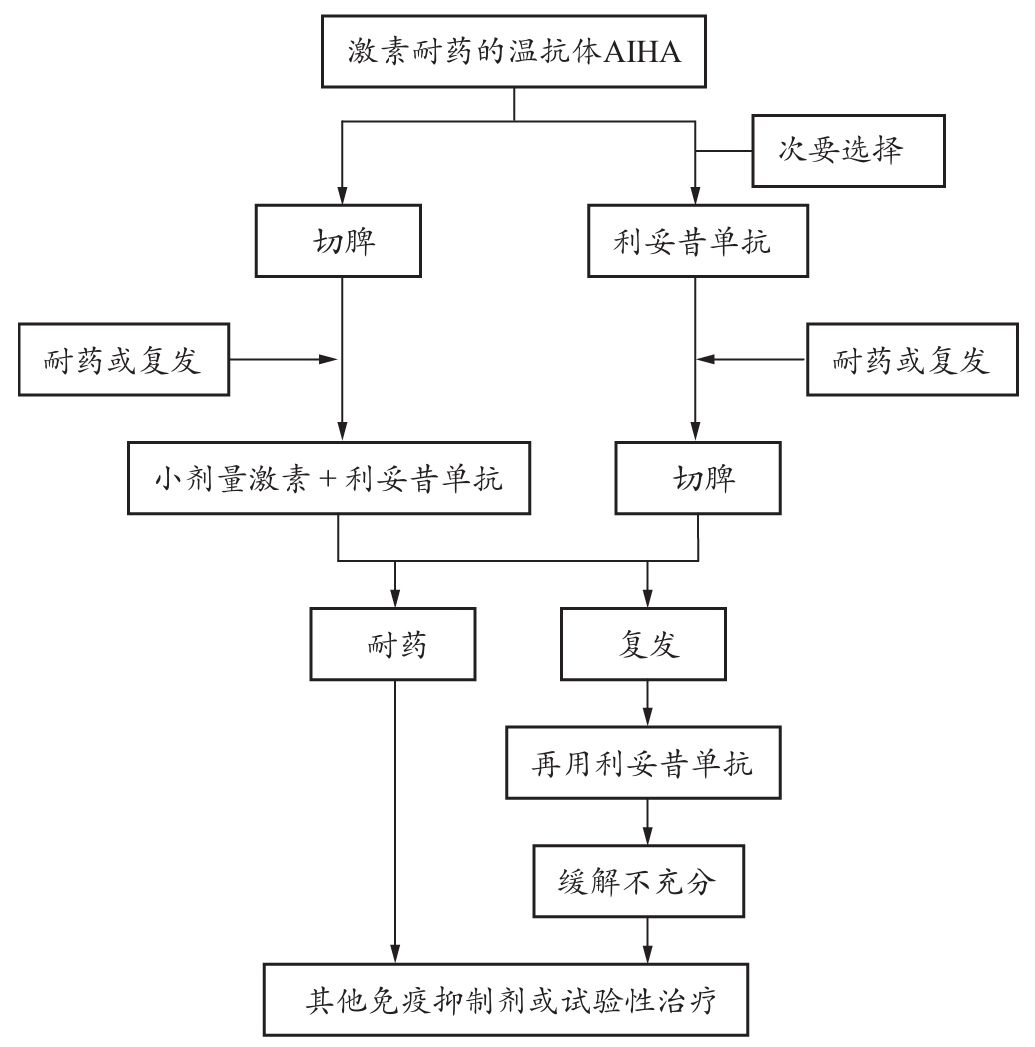
\includegraphics{./images/Image00151.jpg}
 \captionsetup{justification=centering}
 \caption{激素耐药的温抗体型AIHA的治疗流程}
 \label{fig5-2-1}
  \end{figure} 

【治疗方案】 治疗原则:去除病因,早期治疗;坚持治疗;维持治疗。

1.
病因治疗 积极寻找病因,治疗原发病,感染所致的AIHA大多可治愈。继发于卵巢囊肿,畸胎瘤等手术后可治愈,继发于造血系统肿瘤的患者,积极治疗原发病。

2. 药物治疗

(1)糖皮质激素:为首选药物,开始剂量要足,泼尼松1~1.5mg/(kg·d),7~10日内病情改善,起初约80\%患者有效。血红蛋白接近正常时,每周渐减泼尼松用量10~15mg,直至泼尼松20mg,每日1次,每周查血红蛋白及网织红细胞计数,若稳定每周减泼尼松2.5mg,至5~10mg,每日1次,或隔日应用泼尼松10~20mg维持治疗6个月,逐渐停药。撤除激素后成人20\%~35\%患者能获长期缓解。如果在减药过程中或停药后疾病复发,则泼尼松剂量需增加至40~60mg,每日1次。治疗3周无效或泼尼松维持量需在15mg/d以上则需换其他疗法。发生感染往往诱使溶血加重,增加药量,同时加强有针对性的抗生素治疗。

糖皮质激素的作用机理:①作用于淋巴细胞及浆细胞,抑制抗体产生。②改变抗体对红细胞膜上抗原的亲和力。③抑制了巨噬细胞上的IgG及C3受体,或抑制这些受体与红细胞相结合。一般在用药后4~5日,网状内皮系统清除受抗体或补体致敏红细胞的能力即见减退。

(2)免疫抑制剂适应证:①对糖皮质激素及脾切除治疗不能达缓解。②有脾切除禁忌证。③对治疗无效的或必须依赖大剂量激素(泼尼松15mg/d以上者)维持者切脾禁忌,或者切脾无效者均可有使用。治疗期间必须观察血象,至少每周检查1次,应注意骨髓抑制、严重感染。

常用的有:①硫唑嘌呤:是一种对T淋巴细胞抑制作用强烈的免疫抑制剂,体内排泄缓慢,有较高的持久作用,可延长激素的治疗效果。一般剂量为50~200mg,每日1次,或80mg/m$^2$
,有效率50\%左右。由于其胃肠道耐受性和骨髓抑制小,所以在临床上应用较广泛;②环磷酰胺(CTX):剂量为50~150mg,每日1次,或60mg/m$^2$
,可同时合用激素。也有报道用大剂量的CTX50mg/(kg·d),连用4日,和粒细胞集落刺激因子(G-CSF)治疗9例难治AIHA,结果6例达完全缓解(血红蛋白正常),3例达部分持续性缓解(Hb达100g/L以上),平均随访15个月无复发者。血液学缓解后,先减少糖皮质激素剂量,后减少免疫抑制剂至维持剂量,如硫唑嘌呤25mg隔日1次或每周2次维持,治疗需3~6个月。

用药期间注意观察骨髓抑制等副作用。一种免疫抑制剂治疗4周如效果不佳,则可略加大剂量或改用其他制剂,但必须注意血常规和肝肾功能。

(3)大剂量丙种球蛋白0.4~1.0mg/(kg·d),连用5日,起效时间为3周,大多患者需超过1个疗程的治疗。对小部分IgG介导的免疫性溶血性贫血有一定疗效,但疗效短暂。推荐用于常规治疗无效者。Flores等统计73例温抗体型AIHA的对大剂量丙种球蛋白的效果,结果有效率39.7\%,而效果佳与肝大(伴或不伴脾肿大)和治疗前血红蛋白低明显相关。

(4)达那唑:一般在激素治疗无效,或在激素减量时联合应用;作用时间短暂,必要时可重复使用,其他药物治疗无效时可减用。但该药对肝脏有毒性,需定期监测肝功能。Piqnon报道80\%最初有效,但只有60\%长期(随访21个月)有效。剂量600mg,每日1次,同时泼尼松20~30mg,每日1次,待溶血减轻,达那唑逐渐减量直至停用。

(5)环孢素A(CsA):用于治疗糖皮质激素或切脾治疗无效的病例效果也较好。常用剂量为5mg/(kg·d),分次口服,连用6日后改为3mg/(kg·d)维持。其作用机制为:①抑制细胞介导的同种或自身免疫反应;②抑制T细胞生成,阻断与细胞免疫有关的淋巴因子产生抑制T细胞依赖性抗原刺激抗体的反应。不良反应主要为神经毒性。我国天津血液病研究所采用CsA1~3mg/(kg·d),泼尼松0.5~1.0mg/(kg·d)和达那唑0.4~0.6g,每日1次,三药联合治疗18例难治AIHA和Evans综合征患者。血红蛋白正常后CsA逐渐减量,疗程1~2年。结果发现可以降低溶血的复发率,延长缓解期。

(6)霉酚酸酯(MMF):是一种高效的、选择性、非竞争性抑制次黄嘌呤磷酸脱氢酶的抑制剂,阻断DNA合成,抑制T细胞、B细胞的增殖。近期有些学者用该药治疗AIHA也取得较好的疗效。Howard等观察了10例患者,4例AIHA,6例特发性血小板减少性紫癜,剂量为500mg,每日1次,2周后增加到2g,每日1次,所有的AIHA均有很好的反应和部分缓解。MMF可以作为一种有效的二线免疫抑制药。

3. 生物治疗

(1)美罗华:是直接抗B淋巴细胞表面抗原CD20的单克隆抗体,多用于治疗B细胞淋巴瘤。根据其能清除B细胞上抗体的能力,包括红细胞上的自身抗体的清除。目前有数据显示15例温抗体AIHA对常规治疗无效的儿童,采用美罗华每周375mg/m$^2$
,连续2~4周,随访13个月后,13例(87\%)有效。不少文献报道也支持AIHA应用美罗华。

(2)Cammpath-1H:是人源化的针对CD52的单克隆抗体,IgG1型。Marsh等用该药治疗21例对常规治疗无效的免疫性血细胞减少症(包括AIHA、纯红再障和特发性血小板减少性紫癜),第1周成人首次为3mg,逐渐加量至10mg,在患者耐受的情况下用至30mg。结果14例有效,尽管有7例复发,但多数能停止应用激素或减少激素的用量。该药的毒副作用与美罗华相似。

(3)造血干细胞移植:目前已有学者开展治疗对激素依赖的AIHA,我国肖毅等采用美罗华(CD20单抗)进行体内净化以清除异常的B细胞克隆,阻断自身抗红细胞抗体产生后,进行自体外周干细胞移植治疗1例激素依赖的AIHA。预处理方案为CTX50mg/(kg·d),连用4日,+1d和+8d给予美罗华375mg/m$^2$
体内净化,随访13个月,患者Coombs试验阴性,血红蛋白、网织红细胞及胆红素均正常。而异基因造血干细胞移植因治疗相关死亡率高,故临床上并未广泛应用。

4. 手术治疗

(1)脾切除适应证为:急性期患者,糖皮质激素治疗效果差或无效;低剂量糖皮质激素维持治疗下,有严重并发症或溶血反复发作者;需要高剂量糖皮质激素维持治疗(泼尼松15mg,每日1次以上者)。脾切除适用于中青年原发性温抗体AIHA。最初约50\%对脾切有很好的效果,但仍有部分患者需小剂量的泼尼松<15mg,每日1次,维持血红蛋白的水平。晚期疾病复发可能是抗体生成增多和肝内潴留增加所致。脾切除后菌血症的发生率为3.2\%,死亡率达1.4\%,术前应用肺炎球菌和脑膜炎球菌疫苗可以降低菌血症的发生率和死亡率。对是否需要预防性应用抗生素仍有争议,支持者建议青霉素、阿莫西林和复方新诺明交替应用预防。但脾切除的患者一旦发热,及时给予抗生素。

(2)脾动脉栓塞:远期疗效不如脾切除。

5. 其他治疗

(1)血浆置换:可迅速清除自身抗体、补体、免疫复合物及胆红素,改善临床症状,温抗体型疗效差,仅适用于抗体滴度高,危重的溶血危象而其他治疗无效时。

(2)输血:溶血危象或贫血严重的可输洗涤红细胞。因血清中高滴度的自身抗体,常发生配血困难及输血后溶血加重,当出现配血不相容时,需去除IgG抗体再进行ABO配型,但情况危重而配血困难,可给予“O”型的洗涤红细胞悬液。对有妊娠史和输血史(尤其近3个月)的,需鉴定存在多种自身抗体。输血必须审慎,予浓缩的洗涤红细胞输入为宜。

(3)并发叶酸缺乏者:口服叶酸制剂。

【疗效观察与随访】

1.
观察指标 常见症状与体征、血常规、网织红细胞、血红素测定、Coombs试验、血红蛋白尿等。

2. 疗效标准

(1)温抗体型AIHA:

1)完全缓解:临床症状消失,红细胞数、血红蛋白\textgreater{}80g/L,网织红细胞<5\%,血清胆红素测定≤34μmol/L,抗球蛋白试验阴性,或仍为阳性,但效价较治疗前明显降低。

2)部分缓解:临床症状基本消失,血红蛋白及网织红细胞百分率均在正常范围,血清胆红素测定在正常范围,直接和间接抗球蛋白试验转为阴性。

3)无效:临床症状及血象未能达到明显进步者。

(2)冷凝集素综合征:

1)痊愈:继发于支原体肺炎、传染性单核细胞增多症者,原发病治愈后,CAS亦治愈。此时,症状消失,无贫血,DAT-C3型阴性,冷凝集素效价正常(<1∶40)。

2)完全缓解:原发病及继发于目前尚不能治愈而能缓解的疾病,基础病缓解,CAS亦缓解。症状消失,无贫血,DAT阴性,冷凝集素效价正常。

3)部分缓解:症状基本消失,血红蛋白未恢复正常,但较治疗前上升≥20g/L,冷凝集素仍高于正常但较治疗前效价下降\textgreater{}50\%。

4)无效:临床表现及实验室检查无好转或加重。

3.
随访 注意病情观察,观察症状体征等变化,避免致病因素,避免合并症、并发症。必要时复查相关检测指标。

【治疗经验与解析】

1.
糖皮质激素为首选用药,但应注意开始剂量要足,减量不宜太快,维持时间要长,必要时可与免疫抑制剂合用,但要注意骨髓抑制,至少每周复查1次血象。

2. 积极寻找病因,治疗原发病。

3.
预后评价 温抗体型AIHA原发初治患者多数用药后反应良好、月余至数月血象可恢复正常,但需维持治疗。反复发作者疗效差,病程数月至数年不等,病死率约50\%。继发者预后随原发病而异,继发于感染者控制感染后即愈;继发于胶原系统疾病或肿瘤者预后较差,Evans综合征也难以治愈,可死于出血。CAS较温抗体型AIHA好,大多患者能耐受轻度贫血,病程相对良性,均能长期存活,不影响寿命。对劳动能力影响较小,严重感染或严重贫血者预后差。

\paragraph{遗传性球形红细胞增多症}

遗传性球形红细胞增多症(HS)是一种较常见的红细胞膜有先天性缺陷的一种溶血性贫血。其临床特点为贫血、黄疸、脾肿大、血液中球形红细胞增多,病程呈慢性贫血经过并伴有反复急性发作的溶血。此病世界各地均有发现,发病率为20~30/10万人口。此病在我国并不少见,男女均可发病,患病的概率也相同。HS主要通过常染色体显性遗传,但也有部分患者在家族中并没有同样的患者,可能是发生了基因突变引起的。

【治疗方案】

1. 轻型者无需治疗,密切随访。或给予对症治疗。

2. 切除脾脏,最好在10岁以后进行。

3. 脾栓塞治疗HS近期疗效良好,远期疗效有待观察。

4. 重度贫血或发生溶血危象时应输红细胞,必要时予输血小板。

5.
再障危象可给予输血和糖皮质激素1mg/(kg·d),分2~3次口服治疗。

6. 补充叶酸5~10mg,口服,每日3次,预防危象发生。

7. 基因治疗。

【疗效观察与随访】

1. 观察指标 常见症状与体征、血常规、网织红细胞等。

2. 疗效标准

(1)临床缓解:贫血及溶血症状消失,血红蛋白达到男性120g/L,女性100g/L以上,网织红细胞降至3\%以下,随访1年以上无复发者。

(2)明显进步:贫血及溶血症状明显改善,血红蛋白保持70g/L以上,不再输血,随访1年以上病情稳定者。

(3)无效:临床症状及血象未能达到明显进步者。

(4)复发:部分病例于术后若干时间重复出现术前之贫血者。

3.
随访 注意病情观察,观察症状体征等变化,避免合并症、并发症。必要时复查血常规。

【治疗经验与解析】

1.
如病情较重,可提前在1岁行切脾手术。切脾者应给予肺炎球菌疫苗和预防性抗生素。发生下列情况之一者应考虑切脾:①贫血影响生活质量或体能活动;②贫血影响重要脏器的功能;③发生髓外造血性肿块。

2.
本病起病的年龄和病情轻重、预后明显相关,如在新生儿或1岁以内发病,病情较重,预后差。而中年以上症状轻微者,预后较好,只需注意一般卫生保健和适当的生活方式等即可。

\subsection{血红蛋白病}

血红蛋白病是由于血红蛋白分子结构异常(异常血红蛋白病),或珠蛋白肽链合成速率异常(珠蛋白生成障碍性贫血,又称地中海贫血)所引起的一组遗传性血液病。临床可表现溶血性贫血、高铁血红蛋白血症或因血红蛋白氧亲和力增高或减低而引起组织缺氧或代偿性红细胞增多所致紫绀。

大多数异常血红蛋白病系一种珠蛋白链中的一个氨基酸发生替代所致。少数可以发生氨基酸缺失、链延长、链融合或2~3个氨基酸替代。迄今为止已发现500多种异常血红蛋白,但多数异常血红蛋白不伴生理功能改变。我国目前发现的异常血红蛋白已有70余种,分布于几十个民族中,仅1/5的异常血红蛋白有生理功能改变,并产生症状。

【治疗方案】

1. 地中海贫血的治疗

(1)限制铁元素的进食:限制含铁药物的使用及限制进食含铁的食物。

(2)输血疗法:以输浓缩红细胞悬液为宜。目前主张高量输血,维持Hb在100g/L以上,可明显改善患者生存质量,感染、骨骼畸形、骨质疏松症及脾肿大等并发症少,且继发性血色病未提前。近来提倡超量输血,即维持Hb(120~150)g/L可延长生存期,而且输血量并不比高量输血多。输血疗法应在2~3岁开始,否则会影响生长发育。

(3)去铁治疗:见“铁粒幼细胞性贫血”。

(4)维生素C:可增强去铁胺的排铁作用,0.2~0.5g/d,可使去铁胺排铁量增加2倍。但应注意,维生素C可加重组织铁的毒性。茶叶中含鞣酸可与铁形成复合物,不利于铁胃肠道的吸收。

(5)脾切除:对巨脾和脾功能亢进者可行脾切除或脾动脉栓塞术,以减轻溶血。切脾指征:脾大6cm以上或脾功能亢进;输血量逐渐增多,每年在250ml/kg以上;5岁以上。切脾后输血量减少,贫血改善。但脾切除的主要并发症为血小板增多,导致血栓形成和感染。所以脾切除后应给予抗生素预防感染1~2周,血小板大于800×10$^{9}$
/L给予阿司匹林,150~300mg/d,分次服用。噻氯匹定500mg/d,分2次,以防血栓。

(6)抗氧化剂治疗:常用维生素E,10~15mg/d,可减轻溶血,长期服用。维生素C可增强维生素E的抗氧化作用,且可增加去铁胺的排铁作用,但同时增加组织铁对心脏的毒性,故不宜用于严重铁负荷过重的。

(7)羟基脲:最新研究认为羟基脲可使有功能的βmRNA的产量增加,使β珠蛋白肽链合成也增加。羟基脲25~50mg/(kg·d),5~7日1个疗程。

(8)造血干细胞移植:异基因造血干细胞移植是目前根治本病的唯一方法。对有HLA相合的同胞供者的重型β地中海贫血可作为首选治疗。肝大,肝纤维化,铁螯合剂治疗不规范是影响骨髓移植预后的三种因素,并根据这三种因素分为三级:Ⅰ级无上述3种危险因素,Ⅱ级有1或2种危险因素,Ⅲ级有3种危险因素。三级患者获得HLA配型相合的造血干细胞移植后无病生存率分别为87\%、85\%和80\%。

(9)其他:中医中药等治疗。

2. 异常血红蛋白病的治疗

(1)镰状细胞贫血:

1)输血:保持含血红蛋白S的红细胞在40\%以内,每3~4周输红细胞1次。为减轻铁负荷,可交换输血即先放血或红细胞单采后再输红细胞。

2)其他治疗方法:改善α链和非α链合成速率的平衡。①激活血红蛋白F的合成:5-氮杂胞苷2mg/kg,口服,每日1次,7日为1个疗程。促红细胞生成素和α-氨基丁酸、安宫黄体酮或静滴丙种球蛋白等。②针对血红蛋白或红细胞膜的抗镰变剂:硫酸锌、氨甲酰磷酸、氰酸盐和表面活性剂泊洛沙姆-188。③降低红细胞内血红蛋白浓度:西替地尔、克霉唑等。④近年来,越来越多证据表明羟基脲可能是维持治疗镰状细胞贫血的理想药物,目前有五大临床试验收集其安全性及疗效信息。羟基脲有效的主要机制在于其为特异性S期细胞毒药物,是核糖核苷酸还原酶的强有力抑制剂,减少碱磷酸去氧核苷酸的产生,最终达到血红蛋白S减少合成的效果。羟基脲20~50mg/kg,分2~3次口服,5日为1个疗程,间隔1~2周可重复使用。⑤基因治疗:有人用siRNA以修复干细胞缺陷的有关基因,取得初步疗效。⑥异基因造血干细胞移植,是目前临床治愈的唯一方法,有HLA相合同胞供体的重型患者为首选治疗。

(2)不稳定性血红蛋白病:目前尚无特效治疗。避免感染,禁服氧化性药物,大剂量维生素E治疗有一定疗效,严重病例应输血并考虑脾切除。

(3)血红蛋白M病:病程经过良性,不影响患者的生活生命,不需治疗。

(4)异常血红蛋白所致贫血者:氧亲和力降低的异常血红蛋白所致贫血者,不需治疗,不能随便服用补血剂。氧亲和力增高的异常血红蛋白患者,若红细胞压积超过60\%,可以放血治疗。

【疗效观察与随访】

1. 观察指标 常见症状与体征,血常规、网织红细胞等。

2. 疗效标准

(1)临床治愈:治疗后血红蛋白达到或接近正常,达到或接近正常人生活质量,治疗结束后持续一年以上,并预期可长期不依赖输血生存。

(2)显效:治疗后血红蛋白上升≥30g/L,生活质量提高,且继续治疗可维持Hb水平。

(3)有效:治疗后血红蛋白上升≥5g/L,但达不到30g/L,生活质量有所提高。

(4)无效:治疗后血红蛋白上升不足5g/L。

3.
随访 注意病情观察,观察症状体征等变化,避免合并症、并发症。必要时复查血常规及网织红细胞。

【治疗经验与解析】

1.
重型β地中海贫血目前总体预后很差,多数于学龄前因继发感染、心力衰竭而死亡。

2. 预防镰状细胞危象:预防并发症最重要。

3. 可用改善循环药物如复方丹参、潘生丁等。

4. 适量补充叶酸。

5.
利用载体将正常β珠蛋白基因导入患者基因组,以矫正基因缺陷,恢复正常表达调控,但由于珠蛋白基因调控的复杂性和基因突变的多样性,目前此项工作仍处于探索中。

\subsection{代谢酶缺陷引起的溶血}

\paragraph{红细胞葡萄糖-6-磷酸脱氢酶缺乏症}

红细胞内戊糖磷酸途径的多种酶可有遗传性缺陷,红细胞葡萄糖-6-磷酸脱氢酶(G6PD)是磷酸戊糖旁路中的关键酶,红细胞G6PD缺乏症是一种较常见的伴性不完全显性遗传性疾病,由于红细胞活性降低和(或)酶性质改变导致溶血性贫血。依据发病诱因的不同,可分为五种临床类型:①新生儿高胆红素血症。②伯氨喹啉型药物性溶血性贫血。③蚕豆病。④感染诱发的贫血。⑤先天性非球形红细胞性溶血性贫血。在我国,G6PD缺乏症是遗传性红细胞酶缺乏症中最常见的一种。

G6PD缺乏是红细胞最常见的代谢性疾病,患者遍及世界各大洲,各民族间发生率有很大差异。国内以广西壮族自治区某些地区、海南岛黎族、云南省傣族为最多,淮河流域以北较少见。

【治疗方案】

急性获得性溶血性贫血 停止接触已知的药物是治疗的关键,由药物引起的轻度贫血可由造血代偿增加而迅速纠正。轻症患者以口服泼尼松1~1.5mg/(kg·d)及维生素和辅助药为主;重症患者可先静脉使用地塞米松冲击治疗和预防并发症。贫血严重可适当输洗涤红细胞,严重者肾上腺糖皮质激素无效情况下可以选择血浆置换术。对感染等诱发的溶血性贫血应迅速控制感染,及时纠正酸中毒。新生儿高胆红素血症患者换血疗法有助于预防胆红素脑病,目前多采用光照疗法或苯巴比妥5mg/(kg·d),分3次口服,疗程5日。

(1)先天性非球形红细胞性溶血性贫血:输血及使用糖皮质激素可改善病情,但脾切除效果不理想,应慎重。

(2)蚕豆病者:应禁食生熟蚕豆,溶血时可以反复输血及用糖皮质激素为主,严重者应注意水和电解质的平衡,积极纠正酸中毒。

(3)其他:维生素E具有抗氧化作用,可作为治疗药物。

【疗效观察与随访】

1.
观察指标 常见症状与体征、血常规、网织红细胞、电解质、血清胆红素、血红蛋白尿、肝肾功能等。

2.
疗效评估 G6PD缺乏为遗传性缺陷,病因属基因缺陷,目前尚无特殊治疗,故无根治标准。但由于G6PD缺乏所致的溶血性贫血,则可通过治疗而使病情减轻或加速恢复。在判断G6PD缺乏所致溶血性贫血的疗效时,应对照其自然病程,不可将疾病本身的缓解当作治疗有效。

3.
随访 注意病情观察,观察症状体征等变化,避免合并症、并发症。定期复查血常规、网织红细胞、血清胆红素、血红蛋白尿等。

【治疗经验与解析】

1.
G6PD缺乏症所致溶血具有自限性,轻症患者给予补液及对症支持治疗。重症患者可输血、补液、纠正酸碱失衡、抗感染,防治休克和急性肾衰竭等。

2. 除非少见的情况,一般G6PD缺乏者不影响其生存。

\section{粒细胞疾病}

\subsection{中性粒细胞增多症和类白血病反应}

中性粒细胞增多症指成年人外周血中性粒细胞绝对值超过7.5×10$^{9}$
/L。中性粒细胞类白血病反应指并非由白血病引起的中性粒细胞极度升高(可达30×10$^{9}$
/L)以上,分类以中性粒细胞为主和(或)出现幼稚细胞类似白血病的临床现象。淋巴细胞、单核细胞及嗜酸性粒细胞形成的类白血病反应较少见,临床上以中性粒细胞类白血病反应为主。中性粒细胞增多症常见病因包括感染、中毒、药物、变态反应、急性失血、炎症和组织坏死、物理和情绪刺激、恶性肿瘤、血液病尤其是骨髓增殖性肿瘤、代谢和内分泌紊乱。中性粒细胞类白血病反应病因与中性粒细胞增多症较类似,常见为感染、外伤、出血、溶血、药物过敏、恶性肿瘤、粒细胞缺乏症恢复期或使用集落刺激因子。患者主要存在原发病的相关临床表现,可有感染灶的相应表现,可有淋巴结、肝脾肿大、贫血等相关体征。反应性疾病骨髓多增生活跃或粒系更为活跃,各系细胞形态比例正常;血液病或累及血液系统疾病有特殊的骨髓象,必要时可进一步行染色体、分子生物学和流式细胞术检测。

【治疗程序及治疗方案】 寻找病因,治疗原发病,可参照各原发病的治疗。

【疗效观察与随访】

1. 观察指标

(1)症状、体征:观察原发病的症状、体征,如感染灶的症状、体温变化;恶性肿瘤的症状、体征。

(2)血常规及外周血涂片:观察白细胞及中性粒细胞的绝对计数、形态变化。

2. 治愈标准 可参照各原发病的疗效标准进行评估。

3. 随访 观察原发病的症状、体征变化,定期复查血常规及外周血涂片。

【治疗经验与解析】

1. 原发病得到控制后白细胞及中性粒细胞计数随之降低并恢复正常。

2. 应分析其病因,不能盲目制定治疗方案。

3. 判定类白血病反应不能轻易排除白血病,以免延误治疗。

\subsection{白细胞减少和粒细胞缺乏症}

白细胞减少是指外周血白细胞绝对计数持续低于4.0×10$^{9}$
/L。中性粒细胞减少指成人外周血中性粒细胞绝对计数低于2.0×10$^{9}$
/L,≥10岁的儿童低于1.8×10$^{9}$ /L或<10岁的儿童低于1.5×10$^{9}$
/L。粒细胞缺乏症指外周血中性粒细胞绝对计数低于0.5×10$^{9}$
/L。中性粒细胞是白细胞的主要成分,中性粒细胞减少常导致白细胞减少。引起粒细胞减少和粒细胞缺乏原因包括:化学物质如细胞毒药物、止痛药、镇静剂、抗甲状腺药、磺胺药、苯等;放射线接触;急慢性感染;系统性红斑狼疮等风湿性疾病等;具有家族史者,粒细胞减少呈长期稳定状态且红细胞及血小板不减少;先天性中性粒细胞减少多在婴幼儿时期起病,伴或不伴发育异常。中性粒细胞减少症多起病缓慢,患者可无症状,多数患者有头晕、乏力、低热、纳差等,是否发生感染与患者对感染的易感性以及中性粒细胞数、中性粒细胞减少的时间和减少的速率相关,此外皮肤、粘膜的完整性、组织的血液供应和营养状态亦是十分重要的影响因素。粒细胞缺乏症患者起病急,可表现为严重感染,出现畏寒、高热、头痛及乏力,常见感染部位为口腔、舌和咽部,可见坏死性溃疡以及肺、泌尿系统、肝胆,肛周皮肤炎症和脓肿,常发败血症。

【治疗程序】 如图\ref{fig5-3-1}所示。

\begin{figure}[!htbp]
 \centering
 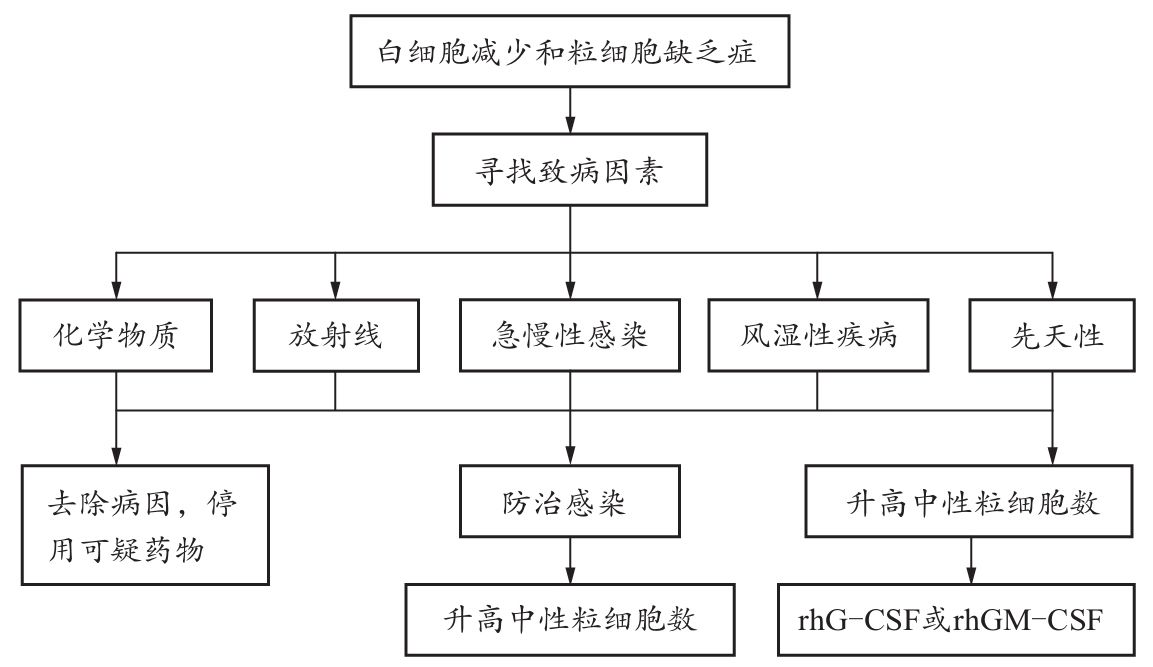
\includegraphics{./images/Image00152.jpg}
 \captionsetup{justification=centering}
 \caption{白细胞减少和粒细胞缺乏症的治疗程序}
 \label{fig5-3-1}
  \end{figure} 

【治疗方案】

1.
一般治疗 积极寻找原发病和可疑的药物或其他致病因素,治疗原发病,去除病因。同时积极防治感染,升高中性粒细胞数。

2. 药物治疗

(1)抗感染治疗:

1)药物治疗原则:轻度中性粒细胞减少者(≥1.0×10$^{9}$
/L)的感染率与正常人无明显差异,不需特别的预防措施。中度减少者(0.5×10$^{9}$
/L~1.0×10$^{9}$
/L)则感染率增加,但因易产生细菌耐药性,不主张预防性应用抗生素。对粒细胞缺乏症患者宜采取无菌隔离措施,同时可选用各种漱口液预防口腔感染,还可适当口服肠道不吸收的抗菌药物(如诺氟沙星、制霉菌素)抑制内源性细菌感染。如患者已发热,常提示感染已经发生,65\%~70\%为细菌感染,须做血、尿、痰或感染病灶分泌物的细菌培养和药敏试验,选用敏感抗生素。在致病菌未找出之前,应立即开始应用广谱抗生素(能覆盖革兰阳性和阴性菌包括铜绿假单胞菌)治疗。广谱抗生素使用效果不佳则考虑真菌感染可能,需使用抗真菌药物。病毒感染可加用抗病毒药物。

2)抗菌药物选用:较常见的细菌为革兰阴性菌(如大肠杆菌、肺炎克雷伯菌、铜绿假单胞菌及变形杆菌),革兰阳性菌(如金黄色葡萄球菌、表皮葡萄球菌、链球菌属),偶尔也有厌氧菌感染。可用的抗生素方案有:第3代头孢菌素与氨基糖苷类(或氟喹诺酮类)合用;单用第4代头孢菌素;单用亚胺培南或与氨基糖苷类(或喹诺酮类)合用;如有金黄色葡萄球菌感染等加用万古霉素。抗生素的剂量宜用足,使其血药浓度达到杀菌水平,对粒细胞缺乏症的患者很重要。经试用抗菌药物治疗3~4日后如病原菌已找到,则根据药敏试验选用敏感抗生素;如未找到,而患者仍未退热,应重复细菌培养及真菌培养,并更换抗生素。如仍无效,须检查患者有无脏器及组织脓肿形成、药物热、病毒感染(肝炎、巨细胞病毒)、寄生虫感染(疟疾、卡氏肺囊虫)等。在排除上述情况后,要考虑隐性真菌感染(念珠菌、曲霉菌等)可能,经验性的使用抗真菌药。

(2)升高中性粒细胞数:

1)造血生长因子:中性粒细胞<1.0×10$^{9}$
/L可使用造血生长因子升高粒细胞数。重组人粒-巨噬细胞集落刺激因子(rhGM-CSF)和重组人粒细胞集落刺激因子(rhG-CSF)适用于各种先天性及获得性粒细胞减少。两药的常用剂量相似,一般2~5μg/(kg·d)就有明显效果,随着剂量增大,效果增强,但当剂量\textgreater{}16μg/(kg·d),效果增加不明显而副作用却增多。两药半衰期短,为2~3小时。常用皮下注射,每日1次或分2次,静脉给药应连续滴注。用药后粒细胞上升效果与造血干细胞损伤程度、恢复增生情况及个体差异性等有关。如果粒细胞缺乏的病因未去除,停药后粒细胞又会迅速下降,故而只能作为支持疗法。常见副作用包括发热、肌肉骨骼疼痛、皮疹、静脉注射后的血栓性静脉炎、血清肌酐暂时性升高等。当剂量<5μg/(kg·d)时,副作用很少出现;而大剂量用药时多见,尤其是用rhGM-CSF的副作用较多,偶可发生毛细血管渗漏综合征。

2)碳酸锂:可增加粒细胞的生成,但对慢性骨髓功能衰竭者无效。剂量为成人每日200~300mg。常见副作用包括胃部不适、瘙痒、水肿等,肾脏疾病患者慎用。

(3)自身免疫性粒细胞减少和通过免疫机制导致的粒细胞缺乏症:可用糖皮质激素、环孢素等免疫抑制剂治疗,其他原因引起的粒细胞减少不宜采用。

【疗效观察与随访】

1.
观察指标 观察体温及各系统感染的症状、体征、血常规、血培养或中段尿培养等。

2. 治愈标准 症状、体征消失,白细胞、中性粒细胞恢复正常,半年内无复发。

3.
随访 观察血常规变化,避免导致白细胞减少的致病因素及使用可疑药物。一旦中性粒细胞数增至1.0×10$^{9}$
/L以上时即可停药。

【治疗经验与解析】

1.
粒细胞缺乏症患者感染的治疗十分重要,粒细胞缺乏症患者一旦发热应立即住院,进行血、尿等标本细菌培养,并立即给予广谱抗菌药物治疗,确定病原体之后改用敏感抗菌药物治疗。

2.
rhGM-CSF除促进粒-单核系祖细胞的增生和分化外,对嗜酸系祖细胞、巨核系祖细胞及红系祖细胞的生长也有刺激作用,所以用药后除中性粒细胞升高外,还可使单核及嗜酸性粒细胞增多。rhG-CSF促进粒系祖细胞增生,缩短分化成熟时间,因而使中性粒细胞迅速增多。此外,两药均能增强中性粒细胞的吞噬杀菌及趋化功能。

\section{淋巴、组织细胞疾病}

\subsection{淋巴瘤}

\paragraph{霍奇金淋巴瘤}

霍奇金淋巴瘤(HL)是一种淋巴系统恶性增殖性疾病,在淋巴组织中具有特征性的Reed-Sternberg(R-S)细胞。HL在世界各地的发病情况差异较大,在欧美国家多发,可占淋巴瘤的20\%左右,我国HL占淋巴瘤的8\%。欧美地区,男性发病多于女性,白人多于黑人,发病年龄呈双峰性,好发于15~34岁的年轻人和大于50岁的老年人;我国发病年龄则呈单峰性。最新的WHO分类将霍奇金淋巴瘤分为淋巴细胞为主型(LPHL)和经典型霍奇金淋巴瘤(CHL)。而CHL可进一步分为结节硬化型、富于淋巴细胞经典型霍奇金淋巴瘤、混合细胞型和淋巴细胞消减型4个亚型。

【治疗程序】 如图\ref{fig5-4-1}、图\ref{fig5-4-2}所示。

\begin{figure}[!htbp]
 \centering
 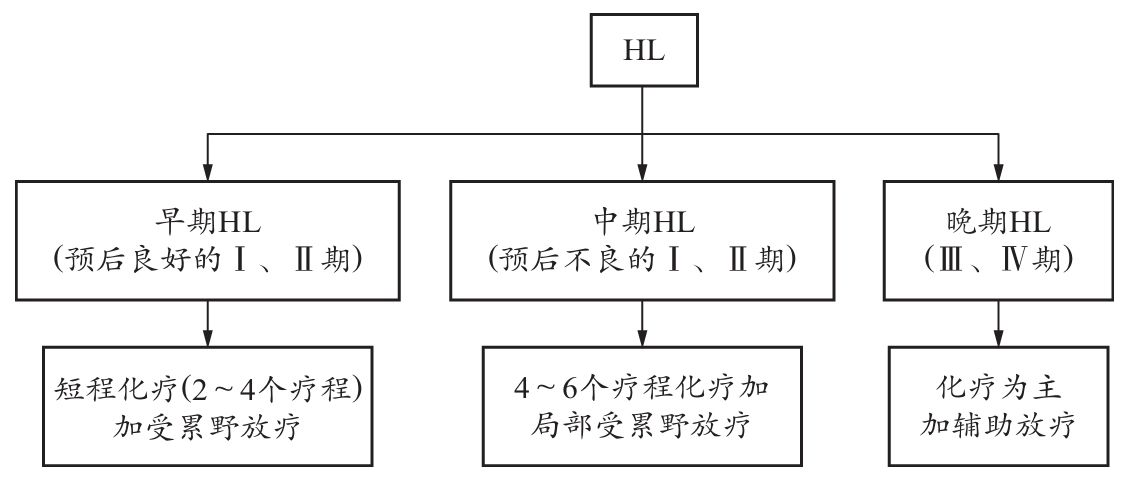
\includegraphics{./images/Image00153.jpg}
 \captionsetup{justification=centering}
 \caption{经典型霍奇金淋巴瘤的治疗流程}
 \label{fig5-4-1}
  \end{figure} 

\begin{figure}[!htbp]
 \centering
 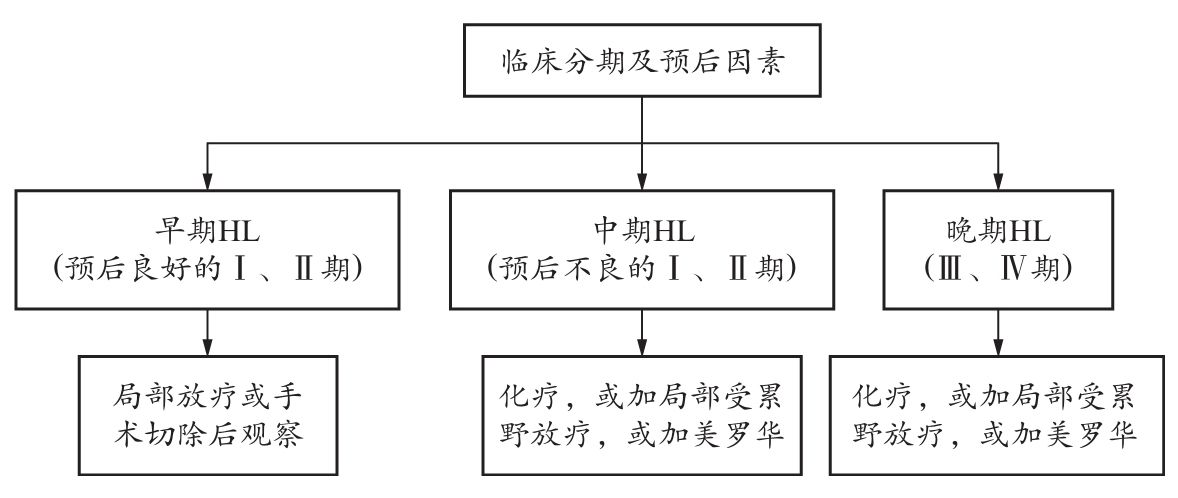
\includegraphics{./images/Image00154.jpg}
 \captionsetup{justification=centering}
 \caption{淋巴细胞为主型的治疗流程}
 \label{fig5-4-2}
  \end{figure} 

【治疗方案】 大多数HL预后较好,甚至可以治愈,为提高患者长期生存的生活质量,选择治疗方案需考虑最大限度地减少治疗相关的远期并发症。通常根据患者的预后选择合理的治疗方案。根据HL的预后因素,一般将Ⅰ期、Ⅱ期HL不伴预后不良因素(如:大纵隔、结外受侵、脾脏受侵、有全身症状者ESR≥30mm/H或无全身症状者ESR≥50mm/H和侵及淋巴结区域数目为1或2个者)称预后良好的Ⅰ期、Ⅱ期HL(或称早期),而将伴有以上一个或多个不良预后因素者称预后不良的Ⅰ、Ⅱ期HL(或称中期),将Ⅲ期、Ⅳ期HL患者称为晚期。

1.
早期HL的治疗 可选用2~4个ABVD方案(±利妥昔单抗)化疗联合受累野放疗;非大肿块者亦可选用2个StanfordⅤ方案化疗联合受累野放疗。ABVD方案每个疗程多柔吡星25mg/m$^2$
,博莱霉素10mg/m$^2$ ,长春花碱6mg/m$^2$ ,达卡巴嗪375mg/m$^2$
,所有药物均在第1日和第15日静脉注射1次,28日为1疗程;若联用利妥昔单抗,于每个疗程第1日375mg/m$^2$
静脉滴注。StanfordⅤ方案:多柔吡星25mg/m$^2$
第1日、15日静脉滴注,长春花碱6mg/m$^2$ 第1日、15日静脉注射,氮芥6mg/m$^2$
第1日静脉注射,长春新碱1.4mg/m$^2$
(最大剂量2mg)第8日、22日静脉注射,博莱霉素5mg/m$^2$
第8日、22日静脉滴注,依托泊苷60mg/(m$^2$
·d)第15日、16日静脉滴注,泼尼松40mg/(m$^2$
·d)第1~28日隔天口服,28日为1疗程。累及野放疗剂量30~40Gy。

2.
中期HL的治疗 可选用4~6个ABVD方案加局部受累野放疗;亦可选用3个StanfordⅤ方案化疗加局部受累野放疗。StanfordⅤ方案中≥50岁者长春花碱自第10周起每周减量1~4mg/m$^2$
,泼尼松第10周起逐渐减量,隔天减10mg。受累野放疗剂量36~40Gy。

3.
晚期HL的治疗 化疗为主加辅助放疗。化疗方案可选用6个ABVD方案,或3个StanfordⅤ方案,或8个BEACOPP方案(或BEACOPP增强方案),化疗后大肿块病灶处放疗36~40Gy。BEACOPP方案(或BEACOPP增强方案)博莱霉素10mg/m$^2$
第8日静脉滴注,依托泊苷100(200)mg/(m$^2$
·d)第1~3日静脉滴注,多柔吡星25(35)mg/m$^2$
第1日静脉滴注,环磷酰胺650(1250)mg/m$^2$
第1日静脉滴注,长春新碱1.4mg/m$^2$
(最大剂量2mg)第1日静脉注射,丙卡巴肼100mg/(m$^2$
·d)第1~7日口服,泼尼松40mg/(m$^2$
·d)第1~14日口服,21日为1个疗程,剂量增强方案需G-CSF支持。

4.
难治或复发的HL的治疗 在初始治疗过程中或3个月内疾病继续进展者称难治性HL,完成完整的治疗疗程3个月后复发者称复发性HL。常用解救方案有MINE、DHAP、ESHAP、GDP、IGEV、异环磷酰胺+长春瑞滨、DEXA-BEAM方案等。对常规解救治疗效果不好的可以用造血干细胞支持下更强烈的化疗。自体造血干细胞移植(ASCT)治疗HL的适应证为复发的HL和原发难治HL。对化疗无反应且治疗过程中进展的HL不适于ASCT治疗;对于化疗反应差但病情较稳定的HL,虽然移植效果相对较差,但仍可考虑移植。一般情况差,年龄\textgreater{}70岁常被认为是ASCT的相对禁忌证。

【疗效观察和随访】

1.
观察指标 常见症状与体征、血常规、骨髓常规、淋巴结活检、肝脾B超检查等。

2. 疗效标准(表\ref{tab5-4-1})

\begin{table}[htbp]
\centering
\caption{修订后的霍奇金淋巴瘤疗效标准(包括PET)}
\label{tab5-4-1}
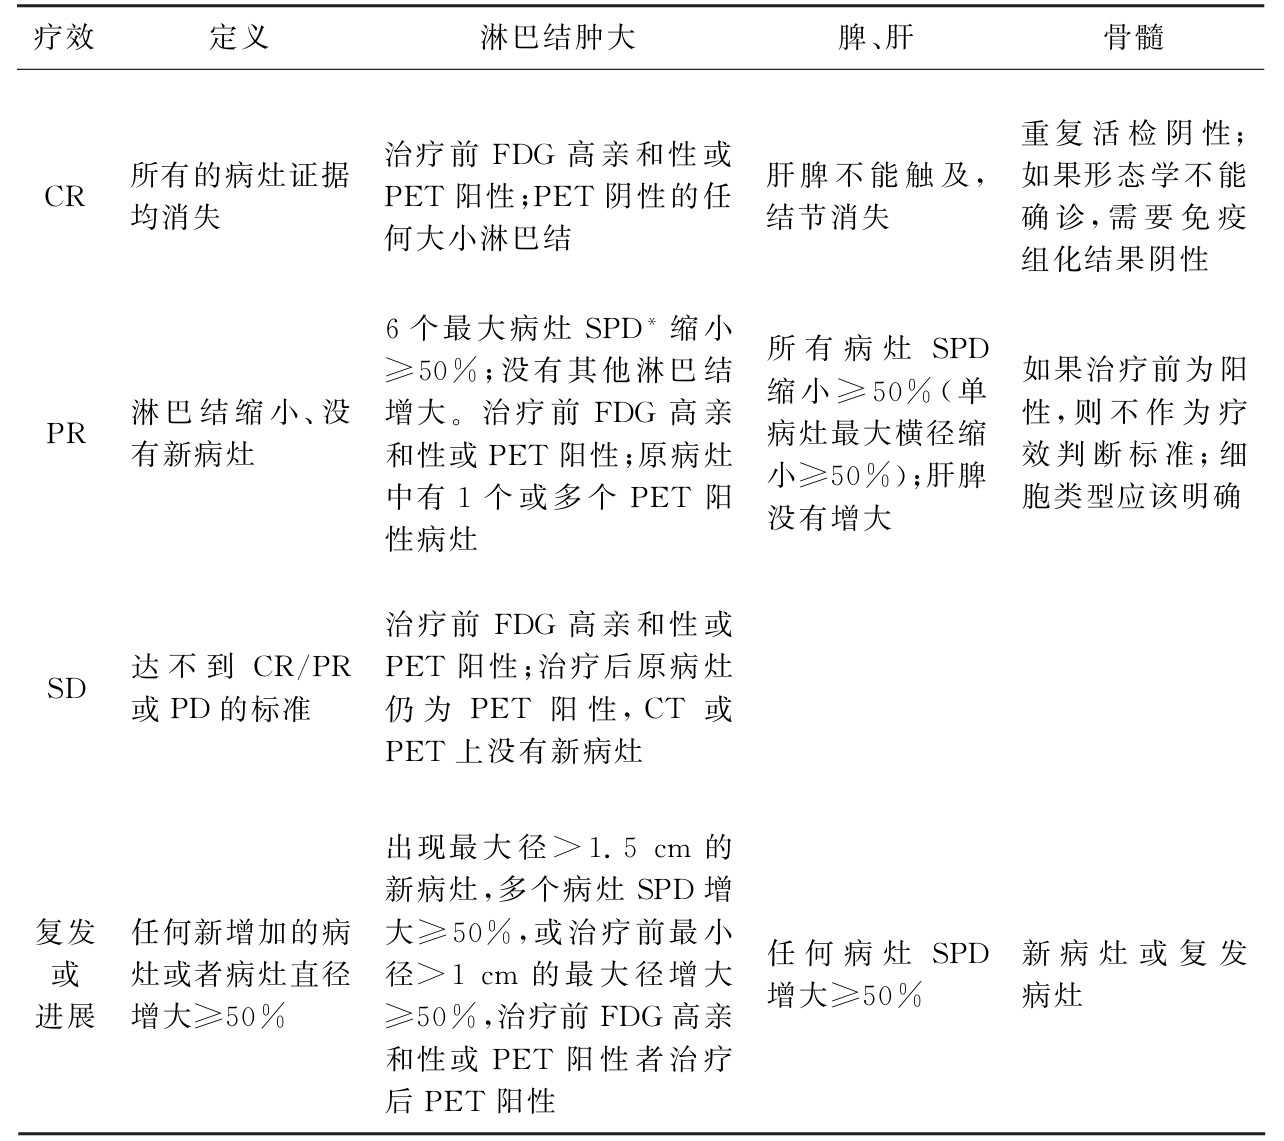
\includegraphics{./images/Image00155.jpg}
\end{table}

注:*SPD:最大垂直径乘积之和。

3.
随访 治疗结束后至少随访5年,其后根据发生晚期并发症如第二肿瘤、心血管疾病等的危险因素每年随访1次。

(1)病史及体格检查:最初1~2年,每2~4个月1次,第3~5年,每3~6个月1次。对于高危人群如接受胸部放射治疗或用博来霉素治疗的考虑每年接种流感疫苗。

(2)实验室检查:血常规、血沉(若发病时升高)、生化,若行颈部放射治疗则每年至少测1次TSH。

(3)胸部影像学检查:最初2~5年,每6~12个月做1次胸部X线片或CT。

(4)腹部或盆腔CT:最初2~3年,每6~12个月1次。

(5)健康咨询:生育、卫生习惯、心理、心血管疾病、乳房自查、皮肤肿瘤风险及关于治疗终点的讨论。

(6)假阳性:由于假阳性可能,PET监测不必常规进行。如何处理不应仅根据PET结果,而应结合临床和病理综合分析。

【治疗经验和解析】

1. 目前常用的分期系统是1989年英国Costwold会议对Ann
Arbor分期的修改而形成新的国际分期方法。常用的分期检查主要有影像学检查、骨髓检查和剖腹探查等。

2.
淋巴细胞为主型(Lymphocyte-predominant,LPHL)和经典型霍奇金淋巴瘤(Classical
HL,CHL)相比,其疾病发展过程和对治疗的反应均有不同。总体而言,LPHL的预后、对治疗的反应要优于CHL,所以在治疗的选择上与CHL也略有不同。此外,LPHL的恶性细胞表达CD20,所以CD20单抗如美罗华常常可以整合到治疗中。

\paragraph{非霍奇金淋巴瘤}

非霍奇金淋巴瘤(NHL)是一种淋巴系统恶性增殖性疾病,包括多种具有不同临床特点的疾病,多累及一至多组淋巴结区。见于各年龄组,随年龄增长发病率增高,男多于女。成人NHL以西欧、美国和中东的发生率为高,东欧和亚洲较低;儿童NHL以非洲和中东的发病率为高,欧洲和美国较低。我国NHL占淋巴瘤的92\%,以中高度恶性NHL和结外原发NHL多见,最常见的病理类型为弥漫性大B细胞淋巴瘤(DLBCL),而滤泡淋巴瘤(FL)比欧美国家少见。

【治疗方案】 NHL因多中心发生的倾向使得临床分期价值和累及野放疗的治疗作用不如HL。治疗策略以全身化疗或联合免疫治疗为主,化疗间歇期或化疗结束后辅助受累野放疗。

1. 化疗

(1)惰性淋巴瘤:B细胞惰性淋巴瘤包括小淋巴细胞淋巴瘤(SLL)、浆细胞样淋巴细胞淋巴瘤、边缘区淋巴瘤和滤泡淋巴瘤(FL)等;T细胞惰性淋巴瘤指蕈样肉芽肿/Sézary综合征。惰性NHL起病隐匿,疾病进展缓慢,化、放疗有效,但不易缓解。Ⅰ期和Ⅱ期患者治疗后存活可达10年,甚至部分患者可自发性肿瘤消退;Ⅲ期和Ⅳ期患者治疗后虽可能多次复发,但中位生存期也可达10年,故在疾病早期主张观察和等待的姑息性治疗原则。化疗或化疗联合放疗是现阶段治疗惰性淋巴瘤的主要手段。COP和CHOP是最经典和常用的方案。COP方案:环磷酰胺750mg/m$^2$
第1日静脉滴注,长春新碱1.4mg/m$^2$
(最大每日剂量2mg)第1日静脉注射,泼尼松60mg/(m$^2$
·d)第1~5日口服,21日为1疗程。CHOP方案:环磷酰胺750mg/m$^2$
第1日静脉滴注,多柔吡星50mg/m$^2$ 第1日静脉滴注,长春新碱1.4mg/m$^2$
(最大每日剂量2mg)第1日静脉注射,泼尼松60mg/(m$^2$
·d)第1~5日口服,21日为1疗程。也可单药苯丁酸氮芥6~12mg/d,分3次口服。若疾病进展不能控制可试用FC方案:氟达拉滨25mg/(m$^2$
·d)第1~3日静脉滴注,环磷酰胺250mg/(m$^2$
·d)第1~3日静脉滴注,28日为1个疗程。

(2)侵袭性淋巴瘤:B细胞侵袭性淋巴瘤包括套细胞淋巴瘤(MCL)、弥漫大B细胞淋巴瘤(DLBCL)和Burkitt淋巴瘤等,T细胞和NK细胞淋巴瘤除了皮肤型这一大组外,大部分均为侵袭性。侵袭性淋巴瘤不论分期均应以化疗为主,对化疗残留肿块、局部巨大肿块或中枢神经系统累及可行累及野放疗作为化疗的补充。常用方案有CHOP(CHOP-14比CHOP-21更有效)、EPOCH、HyperCVAD等方案。EPOCH方案:依托泊苷50mg/(m$^2$
·d)、长春新碱0.5mg/d、多柔吡星10mg/(m$^2$
·d)配置于同一液体中第1~4日持续静脉滴注,环磷酰胺750mg/m$^2$
第5日静脉滴注,泼尼松60mg/(m$^2$
·d)第1~5日口服,21日为1个疗程。Hyper-CVAD方案,A方案(1,3,5,7疗程):环磷酰胺300mg/m$^2$
第1~3日静脉滴注(维持2小时滴注),每12小时1次,Mesna保护,长春新碱1.4mg/m$^2$
(最大每日剂量2mg)第4日、11日静脉注射,多柔吡星50mg/m$^2$
第4日静脉滴注(维持24小时),地塞米松40mg第1~4日、11~14日;B方案(2,4,6,8疗程):甲氨蝶呤1g/m$^2$
第1日静脉滴注(维持24小时),CF解救,阿糖胞苷3.0g/m$^2$
第2日静脉滴注(维持2小时)每12小时1次;每疗程中枢神经系统预防:甲氨蝶呤12mg、阿糖胞苷100mg第2日、7日鞘内注射;所有疗程均G-CSF支持,三周重复(血象允许,2周也可)。

2.
生物治疗 凡CD20阳性的B细胞淋巴瘤均可用利妥昔单抗治疗。利妥昔单抗每次375mg/m$^2$
与化疗联用或单用。

3.
造血干细胞移植 55岁以下、重要脏器功能正常,如属复发、难治或易复发的侵袭性淋巴瘤,化疗后能使淋巴结缩小超过3/4者,可考虑大剂量化疗后进行异基因或自体造血干细胞移植。

【疗效观察和随访】

1. 观察指标 常见症状与体征、血常规、骨髓常规、肝脾B超、淋巴结活检等。

2. 疗效标准 同表\ref{tab5-4-1}。

3. 随访 注意病情观察,观察症状、体征变化,监测血常规、生化及骨髓等。

【治疗经验与解析】

1.
当前的免疫治疗加全身化疗,部分弥漫大B细胞性淋巴瘤(DLBCL)患者可以治愈。而对DLBCL患者而言,通常初始12周的治疗结果往往决定患者最终的治疗效果。所以,在治疗DLBCL初诊患者的过程中,尽可能地使患者按疗程、剂量接受治疗。

2.
对于表达CD20的B细胞NHL如弥漫大B细胞性淋巴瘤(DLBCL)、滤泡性淋巴瘤(FL)、慢性淋巴细胞白血病(CLL)等,抗CD20单克隆抗体美罗华可以提高这些类型淋巴瘤的整体治疗效果。所以,对于有条件的患者,可采用免疫治疗+化疗的治疗方案。

3.
非霍奇金淋巴瘤患者国际预后指标(IPI评分)是基于患者的年龄、体能指数、血LDH水平、结外病变数目和AnnArbor分期这5项变量来对患者评分。根据IPI进行危险度分型,0~1为低危,2分为中低危,3分为中高危,4~5分为高危。对侵袭性淋巴瘤,尤其是DLBCL,IPI对治疗策略选择的指导意义较大。

4. 造血干细胞移植常在大剂量化疗后进行。

\paragraph{慢性淋巴细胞白血病}

慢性淋巴细胞白血病(CLL)是一种成熟B淋巴细胞克隆增殖性肿瘤,以形态学成熟的小淋巴细胞在外周血、骨髓、脾脏和淋巴结聚集为特征。世界卫生组织(WHO)分型中,CLL仅限于肿瘤性B细胞疾病,而以前的T细胞CLL(T-CLL)现称为T幼稚淋巴细胞白血病(T-PLL)(Swerdlow等,2008)。CLL是西方国家成人最常见的白血病,占1/3,国内相对少见。临床预后异质性大。

【治疗程序】 如图\ref{fig5-4-3}所示。

\begin{figure}[!htbp]
 \centering
 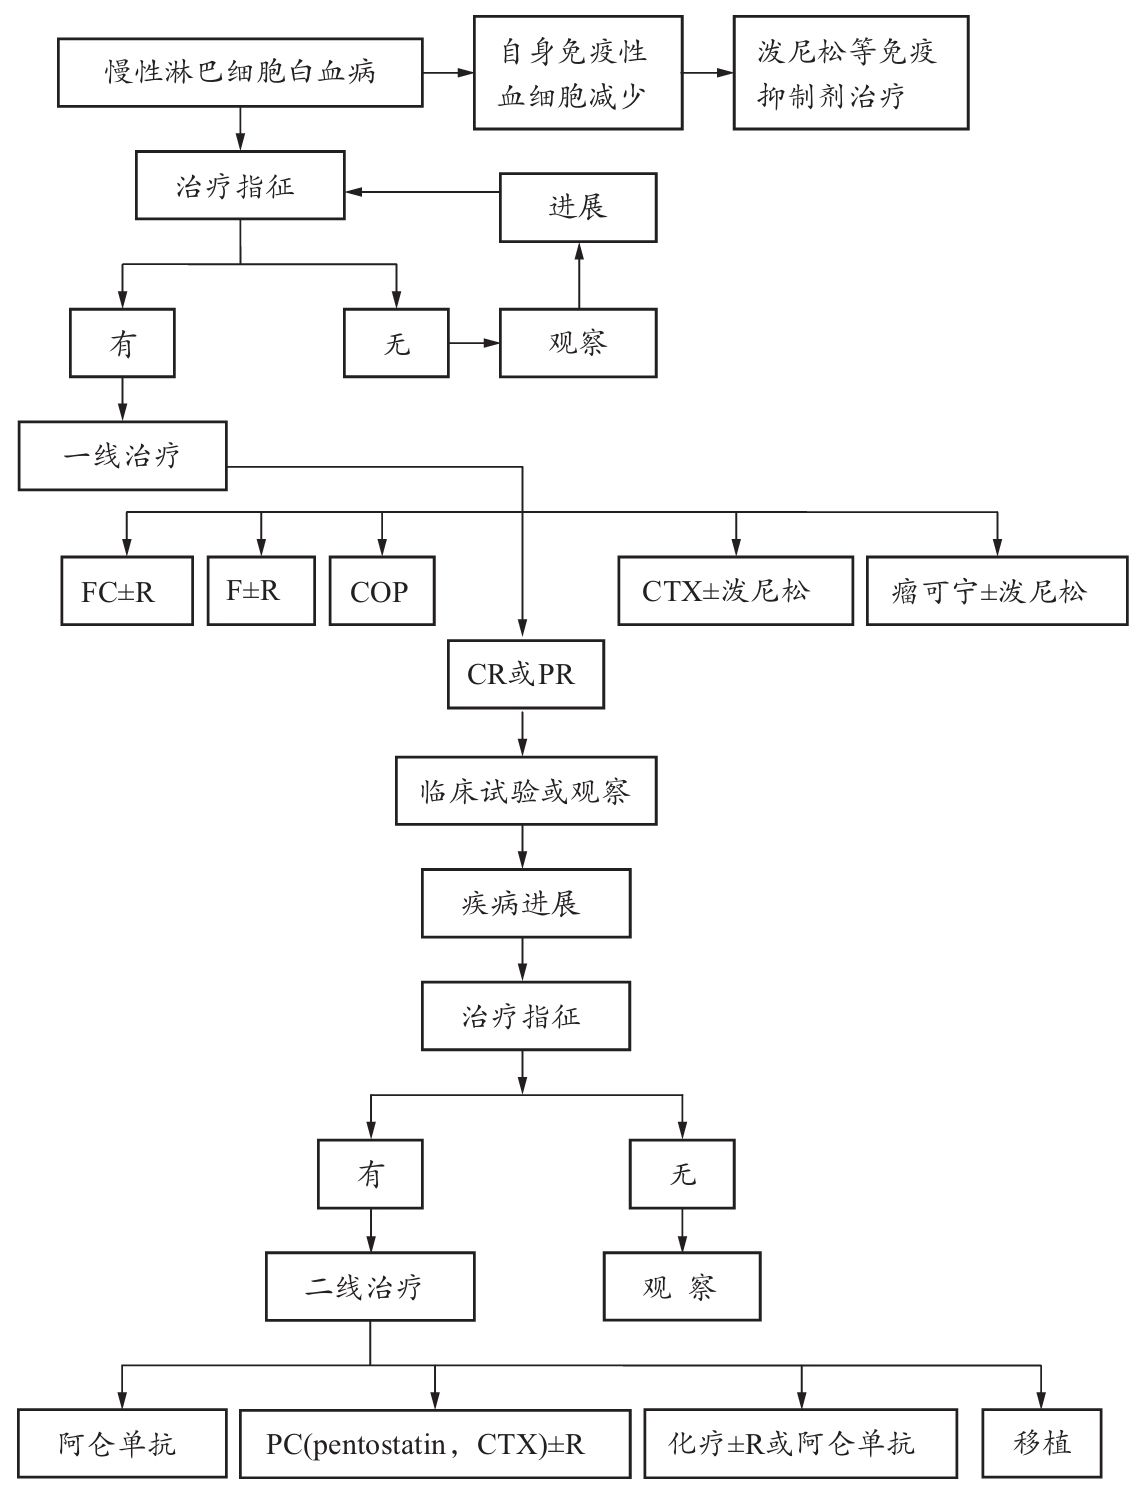
\includegraphics{./images/Image00156.jpg}
 \captionsetup{justification=centering}
 \caption{慢性淋巴细胞白血病治疗流程}
 \label{fig5-4-3}
  \end{figure} 

【治疗方案】

1.
初治患者的治疗选择 对于有治疗指征的年轻(<65岁)患者,应进行FISH检测del(17p),有条件的单位可开展p53突变的检查,突变的意义等同于del(17p)。

(1)对于无del(17p)患者的治疗,按年龄及身体状况进行个体化治疗,选择如下:

1)年轻、无并发症的患者,建议用FC方案,如经济条件许可,首选加用利妥昔单抗的FCR方案。也可应用其他核苷类似物如喷托司汀联合环磷酰胺、利妥昔单抗组成的PCR方案。另外,COP±R、CHOP±R方案也可在部分患者应用,但有效率不及FC为基础的方案高。

2)年龄较大,或合并有严重并发症不能耐受的患者,单药应用氟达拉滨(30mg/m$^2$
,第1~3日静脉滴注,28日为1疗程)、苯达莫司汀、瘤可宁、环磷酰胺或利妥昔单抗均可。

3)合并自身免疫性溶血性贫血(AIHA)的患者,首先应用糖皮质激素控制溶血,如反应不佳则开始针对CLL治疗。避免单用氟达拉滨,但可以在严密监测下应用FC或FCR方案。

(2)伴del(17p)患者的治疗:

1)如年轻有供者,考虑异基因造血干细胞移植,也可采用减低预处理剂量的移植以减轻不良反应。

2)FCR方案。

3)阿伦单抗(CD52抗体):单独应用或与FCR联合。

4)大剂量甲泼尼龙(HDMP):1g/m$^2$
,第1~5日静脉滴注,28日为1疗程。

2.
复发、难治性患者的治疗 对核苷类似物治疗无反应,或虽有反应但停止治疗后6个月以内疾病再次进展,或干细胞移植后1年内疾病进展或复发称为难治性CLL。停止治疗24个月后复发可按原方案治疗;停止治疗后24个月以内复发则按照难治性CLL进行二线治疗。对于未应用氟达拉滨为基础的或未应用利妥昔单抗者可采用FCR方案,对于初治时应用过FCR者可应用阿伦单抗、HDMP治疗。有条件进行移植的患者也可应用异基因造血干细胞移植,对于化疗有效者也可选择自体造血干细胞移植。对于老年或有较严重合并症的患者,保守治疗不失为合适选择。同时疾病复发或进展时应注意排除Richter转化的可能。

3. 巩固维持治疗 维持治疗的意义不明确。

4. 并发症的治疗

(1)并发自身免疫性血细胞减少:

1)首选糖皮质激素,泼尼龙1mg/(kg·d),有效率约75\%,几日至几周起效。

2)静脉丙种球蛋白(IVIG):如果激素治疗7~10日无反应,加用IVIG
0.4/(kg·d),连续5日,起效快而短暂,常需每3~4周重复使用。

3)利妥昔单抗:治疗AHIA的疗效逐渐肯定,并同时治疗CLL本病。

4)其他:如环孢素、脾切除等,部分有效。

(2)感染的防治:如血清IgG<5g/L,每月给予IVIG0.3~0.5g/kg,维持LgG浓度\textgreater{}5~7g/L。注意CLL化疗前后病毒、细菌、真菌感染的预防和治疗,尤其注意乙型肝炎病毒携带者乙肝病毒的监测。

5.
Richter转化的治疗 广义的Richter转化指CLL转化为所有淋巴系统的其他肿瘤。最常见的还是转化为DLBCL,称为Richter综合征。Richter综合征治疗效果明显差于原发的DLBCL,可采用R-CHOP或RICE等DLBCL的二线治疗方案,有条件的可行异基因造血干细胞移植。

【疗效观察与随访】

1.
观察指标 常见症状与体征、血常规、血小板、骨髓常规、肝脾B超检查、淋巴结活检等。

2. 疗效标准(表\ref{tab5-4-2})。

\begin{table}[htbp]
\centering
\caption{CLL的疗效标准}
\label{tab5-4-2}
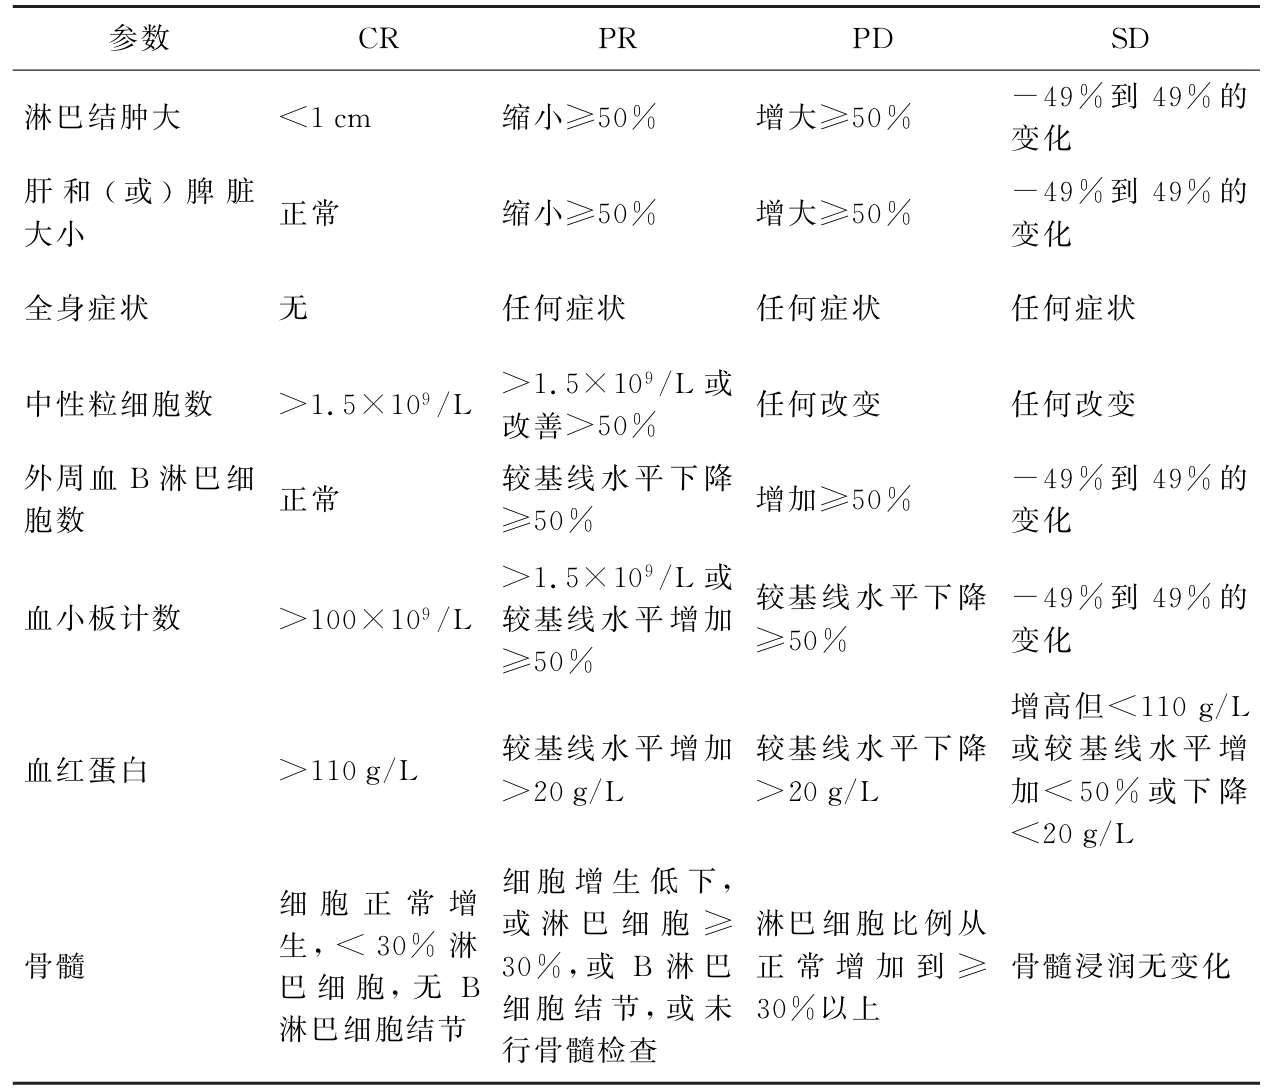
\includegraphics{./images/Image00157.jpg}
\end{table}

3.
随访 注意病情观察,观察症状、体征变化,监测血常规、外周血B淋巴细胞计数及骨髓等。

【治疗经验与解析】

1.
CLL的诊断确定后,首要问题不是选择治疗方案,而是考虑何时开始治疗。一般来说,1/3患者无需治疗,1/3需要即刻治疗,1/3患者诊断时无需治疗、随着病情进展需要治疗。只有RaiⅢ和Ⅳ期或BinetB和C期的患者治疗能够改善预后。

2008年IWCLL提出的CLL开始治疗的标准至少应该满足以下1个条件(Hallek等,2008):

(1)进行性骨髓衰竭的证据,表现为贫血和(或)血小板减少进展或恶化。

(2)巨脾(如左肋缘下\textgreater{}6cm)或进行性或有症状的脾肿大。

(3)巨块型淋巴结肿大(如最长直径\textgreater{}10cm)或进行性或有症状的淋巴结肿大。

(4)进行性淋巴细胞增多,如2个月内增多\textgreater{}50\%,或淋巴细胞倍增时间(LDT)<6个月。当初治淋巴细胞<30×10$^{9}$
/L,不能单凭LDT作为治疗指征。

(5)自身免疫性贫血和(或)血小板减少对皮质类固醇或其他标准治疗反应不佳。

(6)至少存在下列一种疾病相关症状:①在以前6个月内无明显原因的体重下降≥10\%。②严重疲乏[如ECOG体能状态(PS)≥2;不能工作或不能进行常规活动]。③无其他感染证据,发热\textgreater{}38.0℃,≥2周。④无感染证据,夜间盗汗\textgreater{}1个月。

2.
低丙种球蛋白血症或单克隆、寡克隆副蛋白血症本身不是开始治疗的指征。CLL患者可表现为显著的白细胞增高,但是,白细胞聚集相关的症状在CLL患者中罕见。所以,淋巴细胞数不能作为治疗的唯一指标。对部分血小板轻度减少,病情稳定的患者建议暂缓治疗、密切观察,有明显疾病进展时开始治疗。

3.
起始治疗达完全缓解(CR)或部分缓解(PR)的患者随访观察,除非进行临床试验,否则无需进一步治疗。观察过程中疾病进展的治疗原则同起始治疗。二线治疗需考虑缓解持续时间及首次用药。

\subsection{浆细胞病}

\paragraph{多发性骨髓瘤}

多发性骨髓瘤(MM)是一种恶性浆细胞克隆性增生疾病,以骨髓内有恶性浆细胞(骨髓瘤细胞)的增殖与聚集,并分泌单克隆免疫球蛋白(M蛋白)为特征。主要表现为贫血、出血、溶骨性损害、病理性骨折、高钙血症、肾功能损害。欧美国家MM的年发病率约为5/10万人口,中位发病年龄为65岁,40岁以下发病罕见。我国发病率低于欧美国家,年发病率约为1/10万人口,但发病年龄较欧美国家明显提前。几十年来,MM一直采用激素和细胞毒性药物联合化疗,中位生存期3~5年,近年来采用了大剂量化疗和自体造血干细胞移植,及针对瘤细胞和造血微环境的靶向治疗沙利度胺及其衍生物和蛋白酶体抑制剂等,生存期虽有所改善,但迄今为止,MM仍是一种不可治愈的疾病。

【治疗程序】 如图\ref{fig5-4-4}所示。

\begin{figure}[!htbp]
 \centering
 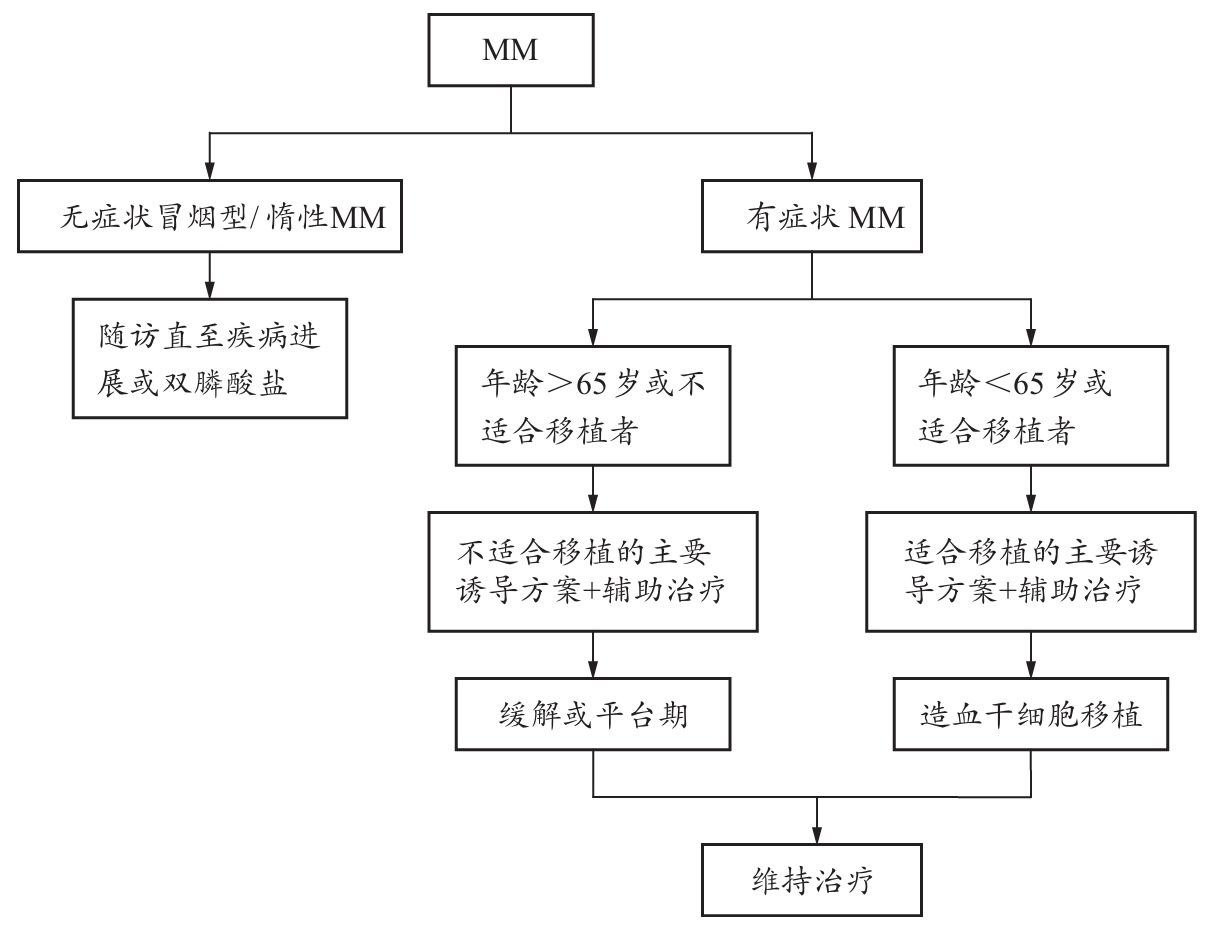
\includegraphics{./images/Image00158.jpg}
 \captionsetup{justification=centering}
 \caption{多发性骨髓瘤的治疗流程}
 \label{fig5-4-4}
  \end{figure} 

【治疗方案】 对无症状、无骨损害、无进展证据的冒烟型MM或ⅠA期患者可暂不治疗,每3~6个月随访检查1次,每年1次骨骼平扫,至病情进展、出现症状时开始治疗。当患者出现血、尿中M蛋白进行性增加、贫血、高钙血症、肾功能不全、骨痛、溶骨性损害、病理性骨折以及髓外浆细胞瘤等症状时开始治疗。

1.
一般治疗 预防感染,加强口腔、外阴护理;发生感染应积极抗感染治疗,必要时予以静脉滴注丙种球蛋白等支持治疗。贫血采用重组人促红细胞生成素(rHuEPO)治疗,EPO开始剂量通常是150U/kg,皮下注射,每周3次,当Hb上升到120g/L时,EPO应该停用或减量。如治疗4~6周后反应不理想,可将剂量提高1倍再治疗6~8周,如Hb未能上升10~20g/L,说明无效,即可停用EPO。防治高尿酸血症,水化碱化尿液,降低高钙血症,纠正电解质紊乱,维持足量尿量,防治肾功能不全,禁用损害肾功能的药物(如非甾体类解热镇痛药物以及静脉造影剂等),肾衰竭时可行血浆置换或血液透析。对于症状性高粘血症,可采用血浆置换作为辅助治疗。

2.
放疗 低剂量放射(10~30Gy)可以作为姑息治疗,用于不能控制的疼痛,即将发生的病理性骨折或即将发生的脊髓压迫。

3.
诱导化疗 由于目前认为含自体造血干细胞移植的治疗方案,可以提高多发性骨髓瘤的总体治疗效果,所以对于适合自体造血干细胞移植的患者,均应推荐在治疗方案中整合自体造血干细胞移植。由于某些烷化剂类药物如马法兰对造血干细胞有明显损害,所以对于适合移植的患者应该避免使用这一类药物。

总体而言,对于适合移植的骨髓瘤患者,要避免在移植前采用对造血干细胞采集有明显影响的化疗方案。而对不适合移植的骨髓瘤患者,既可以采用对造血干细胞采集有明显影响的化疗方案,也可以采用适合移植患者的方案。

对于年龄65岁以上或因基础疾病不适合自体造血干细胞移植(ASCT)的MM患者,除常规以烷化剂为基础的联合诱导方案外,可在原诱导缓解方案基础上加入沙利度胺及其衍生物和蛋白酶体抑制剂等新的药物组合,疗效优于原方案。

对于年龄≤65岁且无移植禁忌者均首先考虑ASCT治疗,应该限制使用烷基化药物和亚硝基脲类骨髓毒性药物,从而避免危害干细胞采集前的干细胞储备。诱导期间尽量加入新型治疗药物以获得高缓解率,尽可能采集足够双次ASCT的干细胞。

(1)不适合移植患者的初始治疗方案:近年来出现的新治疗方案与以往方案相比,总有效率、完全和部分缓解率均有明显的提高,具体的方案包括MPT(马法兰+泼尼松+沙利度胺)、RD(来那度胺+地塞米松)、MPV(马法兰+泼尼松+硼替佐米+地塞米松)、MPR(马法兰+泼尼松+来那度胺)和BD(硼替佐米+地塞米松)方案。而以往的治疗方案与现在的上述方案相比,由于疗效欠佳已经不再作为首选方案。但在一些特定的情况下也可以选择作为患者的初诊方案。这些方案包括MP(马法兰+泼尼松)、VAD(长春新碱+阿霉素+地塞米松)、地塞米松单用方案。部分方案的具体用法见表\ref{tab5-4-3}。

\begin{table}[htbp]
\centering
\caption{不适合移植多发性骨髓瘤患者的诱导方案}
\label{tab5-4-3}
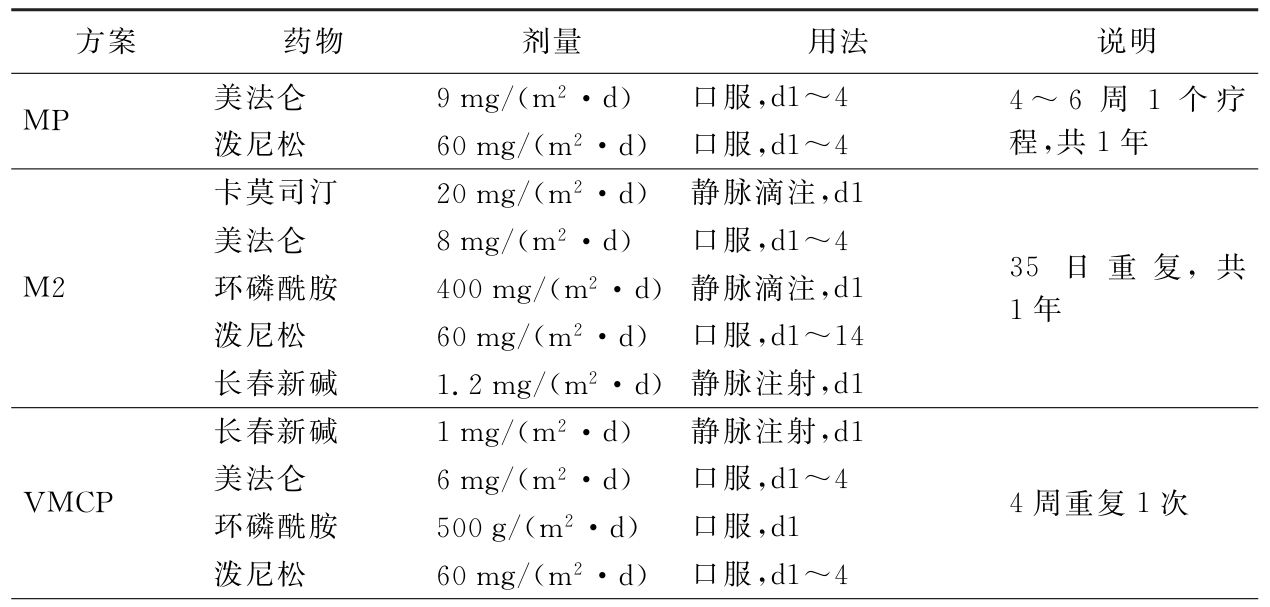
\includegraphics{./images/Image00159.jpg}
\end{table}

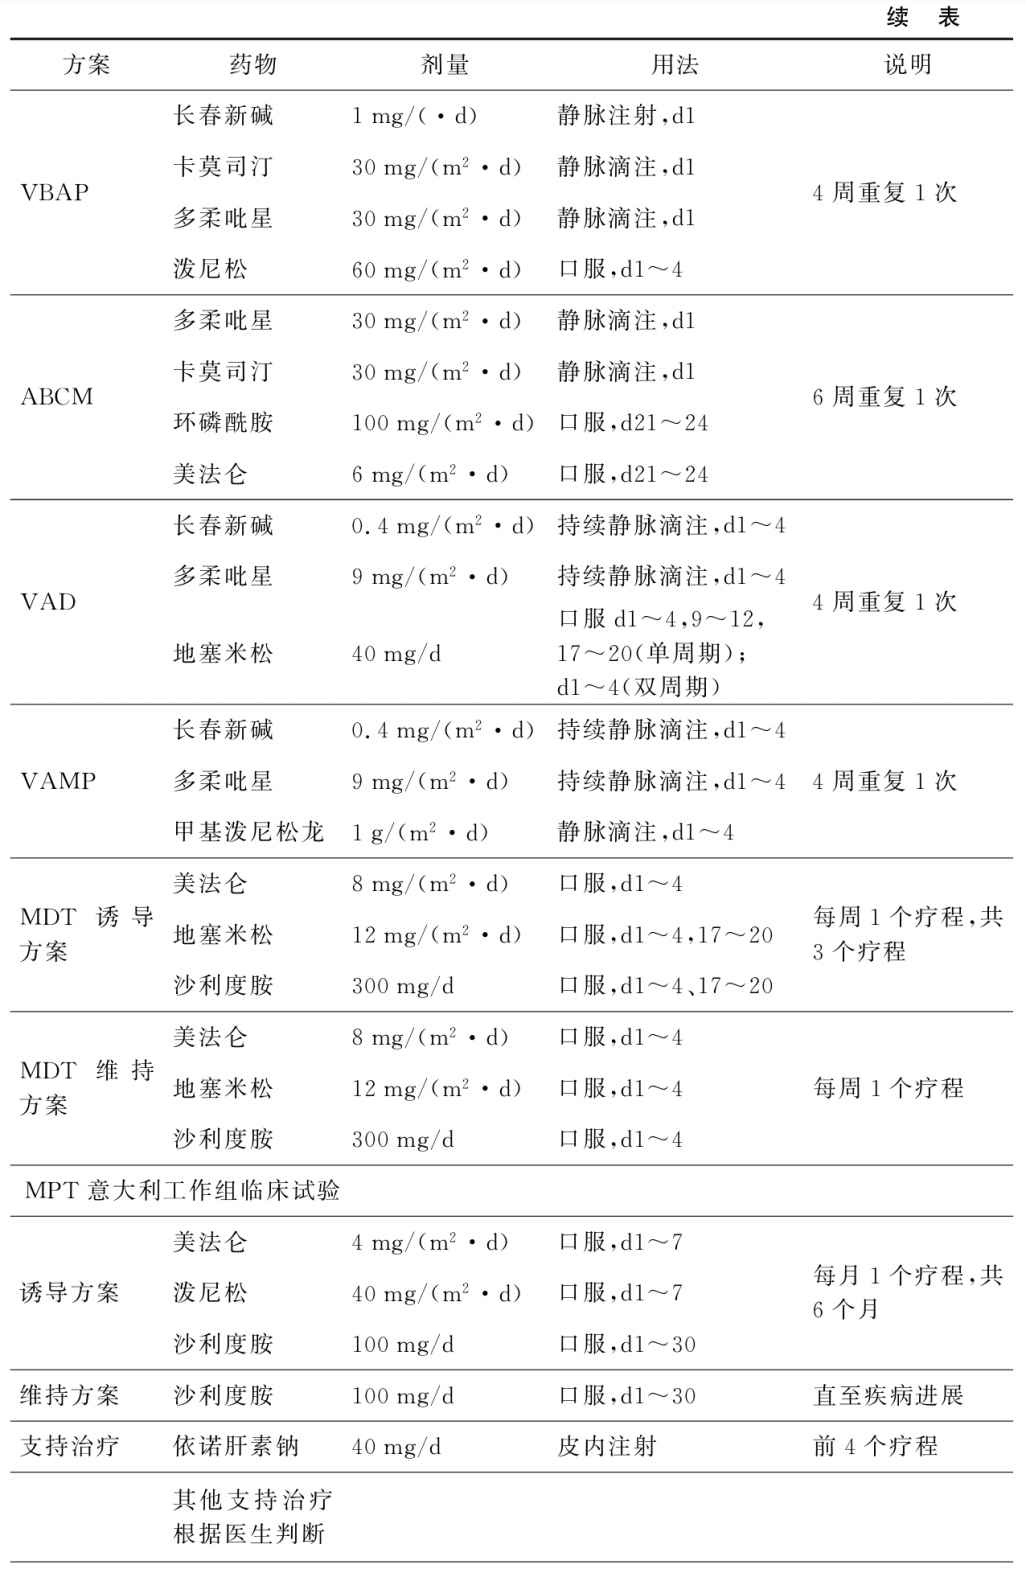
\includegraphics{./images/Image00160.jpg}

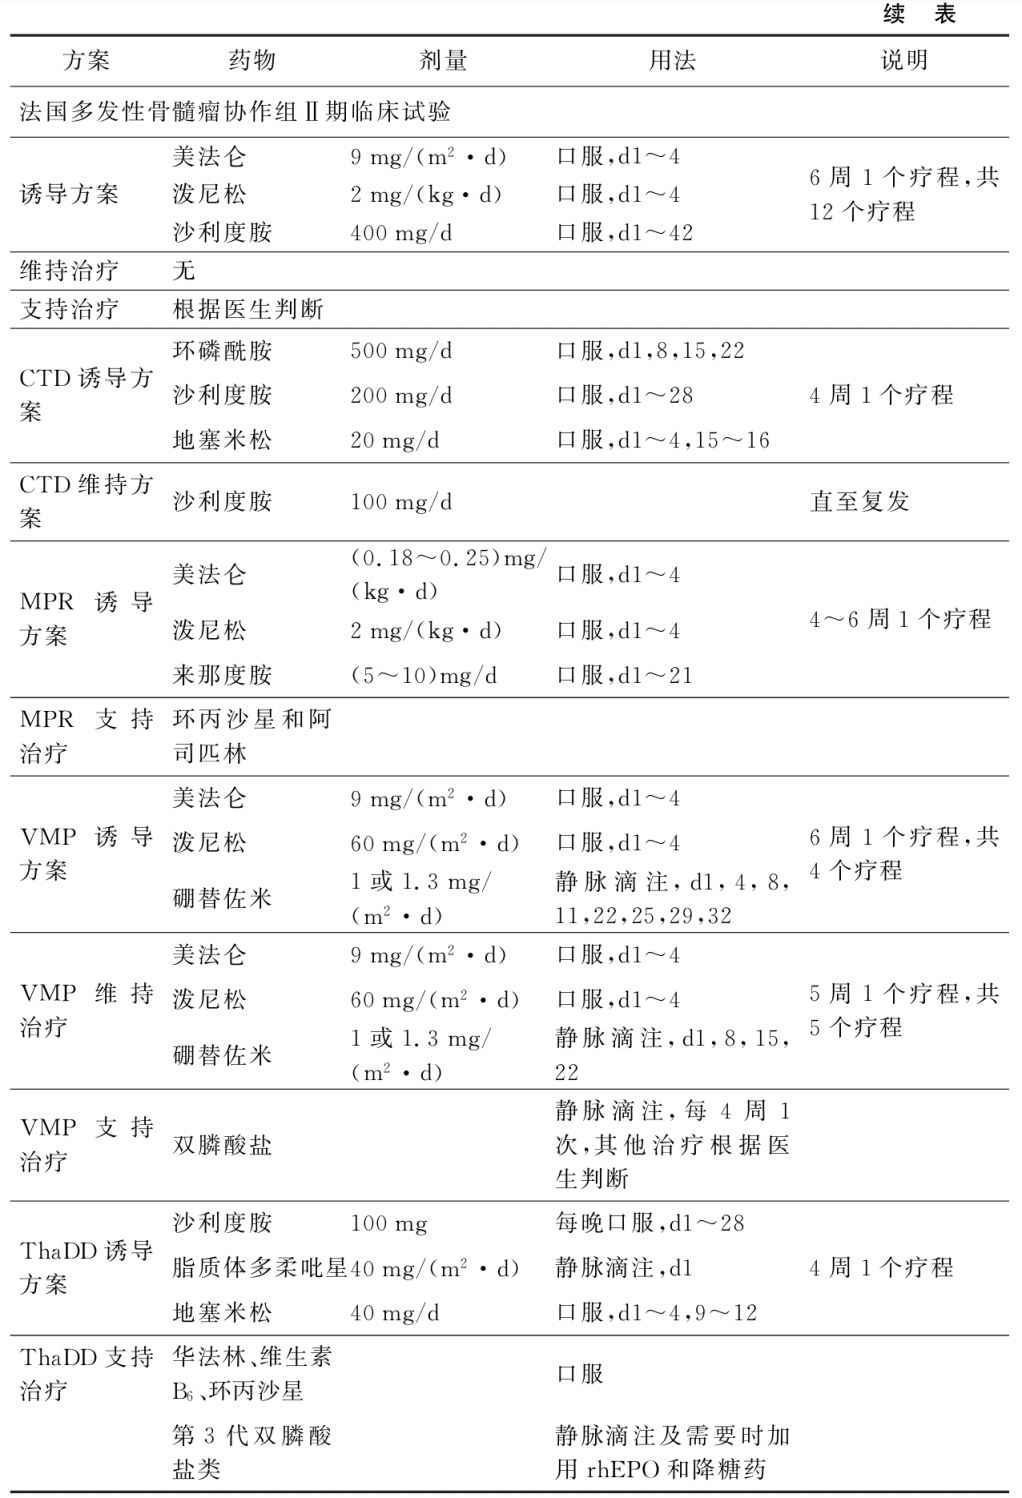
\includegraphics{./images/Image00161.jpg}

(2)适合移植患者的主要诱导方案:对于适合移植患者,要避免在移植前采用对造血干细胞采集有明显影响的化疗方案。对于这一部分患者,移植前治疗方案可以选用BD(硼替佐米+地塞米松)、PAD(硼替佐米+阿霉素+地塞米松)、RVD(硼替佐米+来那度胺+地塞米松)、VTD(硼替佐米+沙利度胺+地塞米松)、RD(来那度胺+地塞米松)。经上述方案治疗后,总有效率、完全和部分缓解率均较以往的传统方案明显提高。在某些特定情况下,也可以在移植前用TD(沙利度胺+地塞米松)、VAD(长春新碱+阿霉素+地塞米松)、DVD(酯质体阿霉素+长春新碱+地塞米松)等方案(表\ref{tab5-4-4})。

\begin{table}[htbp]
\centering
\caption{适合移植多发性骨髓瘤患者的诱导方案}
\label{tab5-4-4}
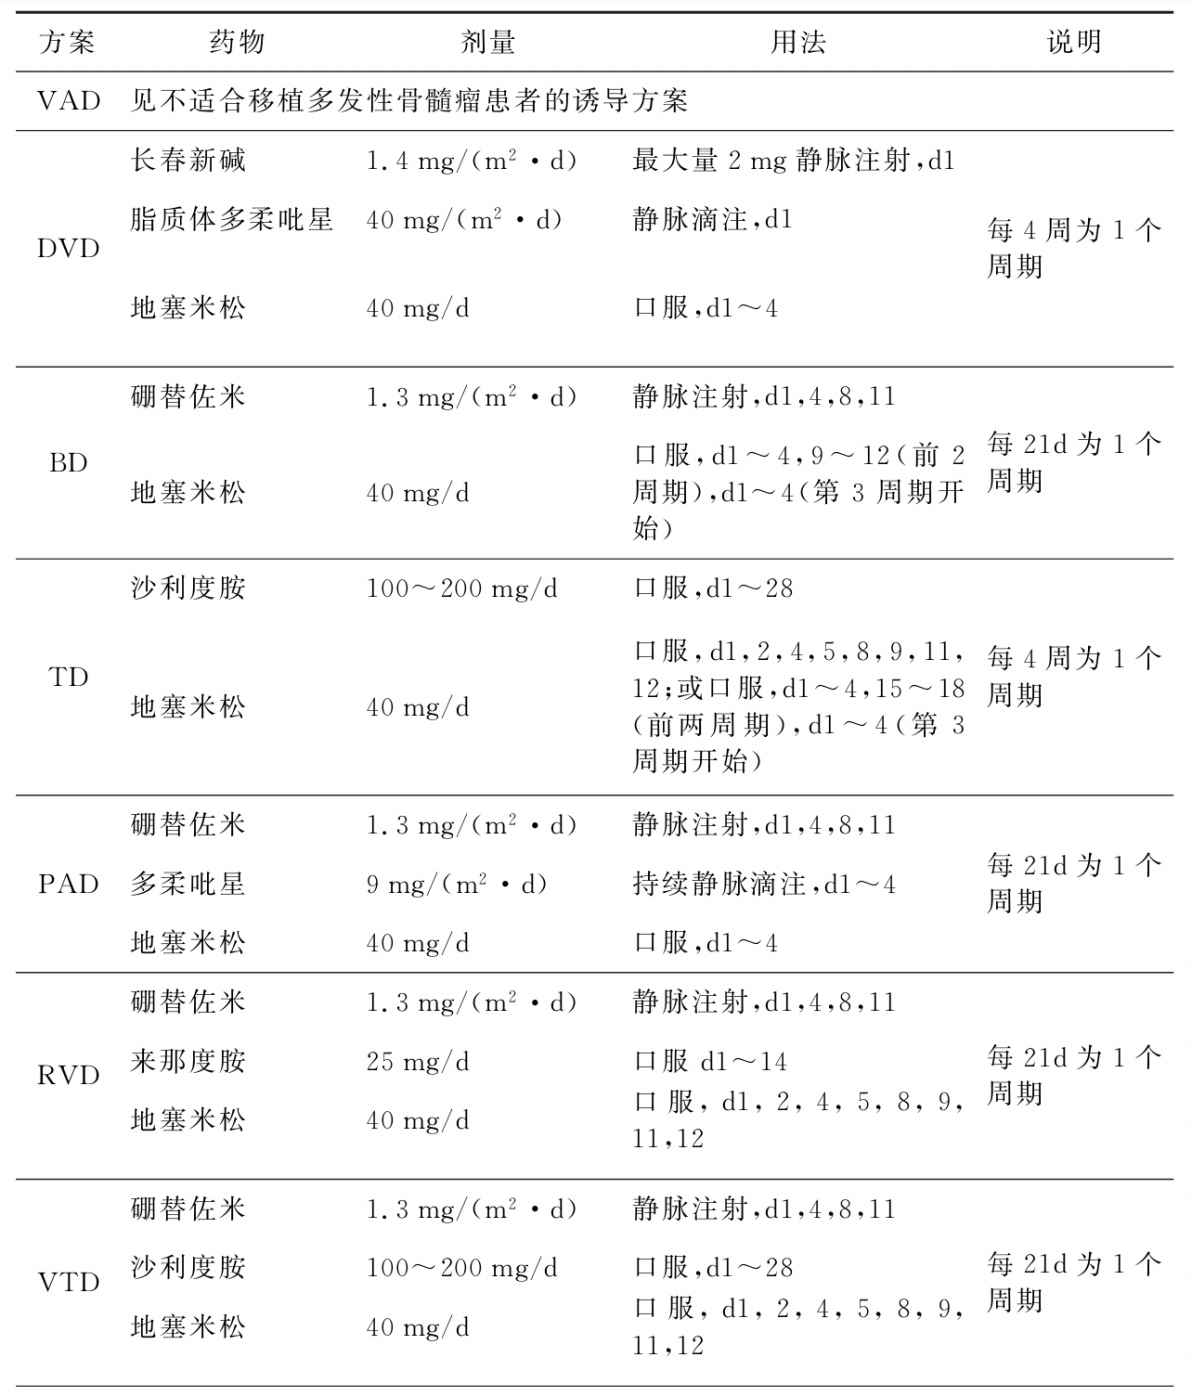
\includegraphics{./images/Image00162.jpg}
\end{table}
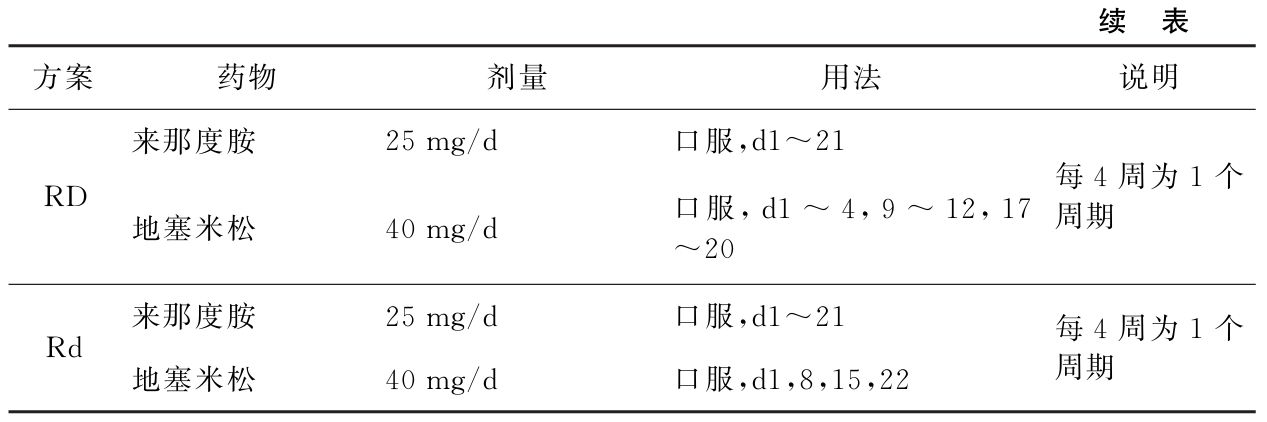
\includegraphics{./images/Image00163.jpg}

4. 维持治疗

(1)沙利度胺:已有MM患者ASCT后采用沙利度胺作为维持治疗的Ⅲ期临床试验,结果表明沙利度胺维持治疗具有一定的生存优势,但这一结果尚未在不适合ASCT的患者中得到证实。

(2)硼替佐米和来那度胺:在近期进行的一些观察性研究中,MM患者ASCT后采用硼替佐米或来那度胺进行维持治疗,初步结果令人鼓舞,但尚需在随机对照研究中进行验证。

(3)糖皮质激素:有报道用泼尼松50mg,隔日1次,作为维持治疗,其无进展生存期及总生存期较无维持治疗组明显延长,提示泼尼松作为维持治疗可能有效。但另有研究表明,采用地塞米松维持治疗者的PFS明显延长,但并不能改善OS。因此,激素作为维持治疗的依据尚不够充分,需要更多的临床研究去证明其益处、安全性和对生活质量的影响。

(4)干扰素:干扰素α(IFNα)300万~500万U,皮下注射,3次/周,对常规或大剂量化疗后平台期的患者及移植后的患者有一定的活性。对传统化疗患者IFN-α维持治疗PFS有所改善,但对总生存期并无延长。移植后IFN-α维持治疗的经验尚不多。干扰素的治疗持续时间尚无定论。主要不良反应有流感样综合征、全身乏力、自身免疫性疾病、阳痿和抑郁等。

5.
难治或复发MM的治疗 国际骨髓瘤工作组(IMWG)将难治与复发性MM定义为:经初始治疗取得微小反应以上的疗效,复发后经挽救性治疗仍发生疾病进展者;或在接受末次治疗后60日内疾病又进展者。当患者在一线治疗中进展或当再重复一线治疗无效时称为难治性MM,需要换其他方案或策略。复发MM患者如发生在一线治疗停止后1年内,换用二线治疗;如发生在1年以上,可选用原方案治疗。既往二线治疗方案见表\ref{tab5-4-5}。随着靶向治疗药物(沙利度胺、硼替佐米和来那度胺)的临床应用,即BD、PAD、RVD、VTD、TD及RD等方案的应用,难治与复发性MM的治疗取得了明显的进步,因此已作为目前二线治疗的主要方案。

\begin{table}[htbp]
\centering
\caption{多发性骨髓瘤二线化疗方案}
\label{tab5-4-5}
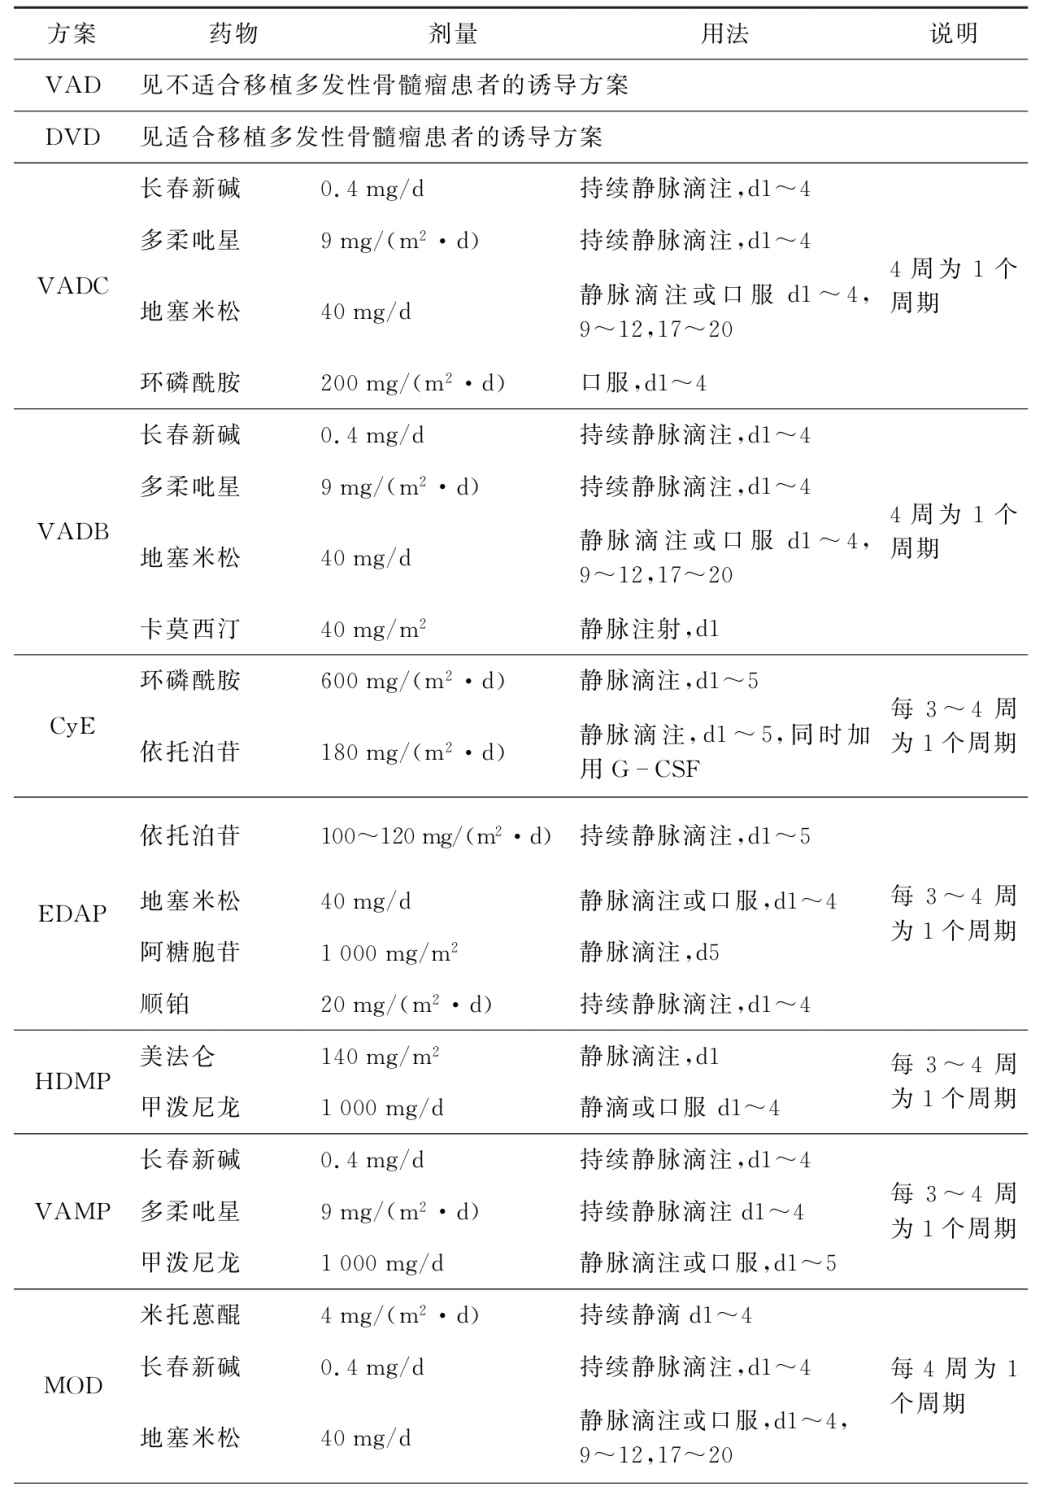
\includegraphics{./images/Image00164.jpg}
\end{table}
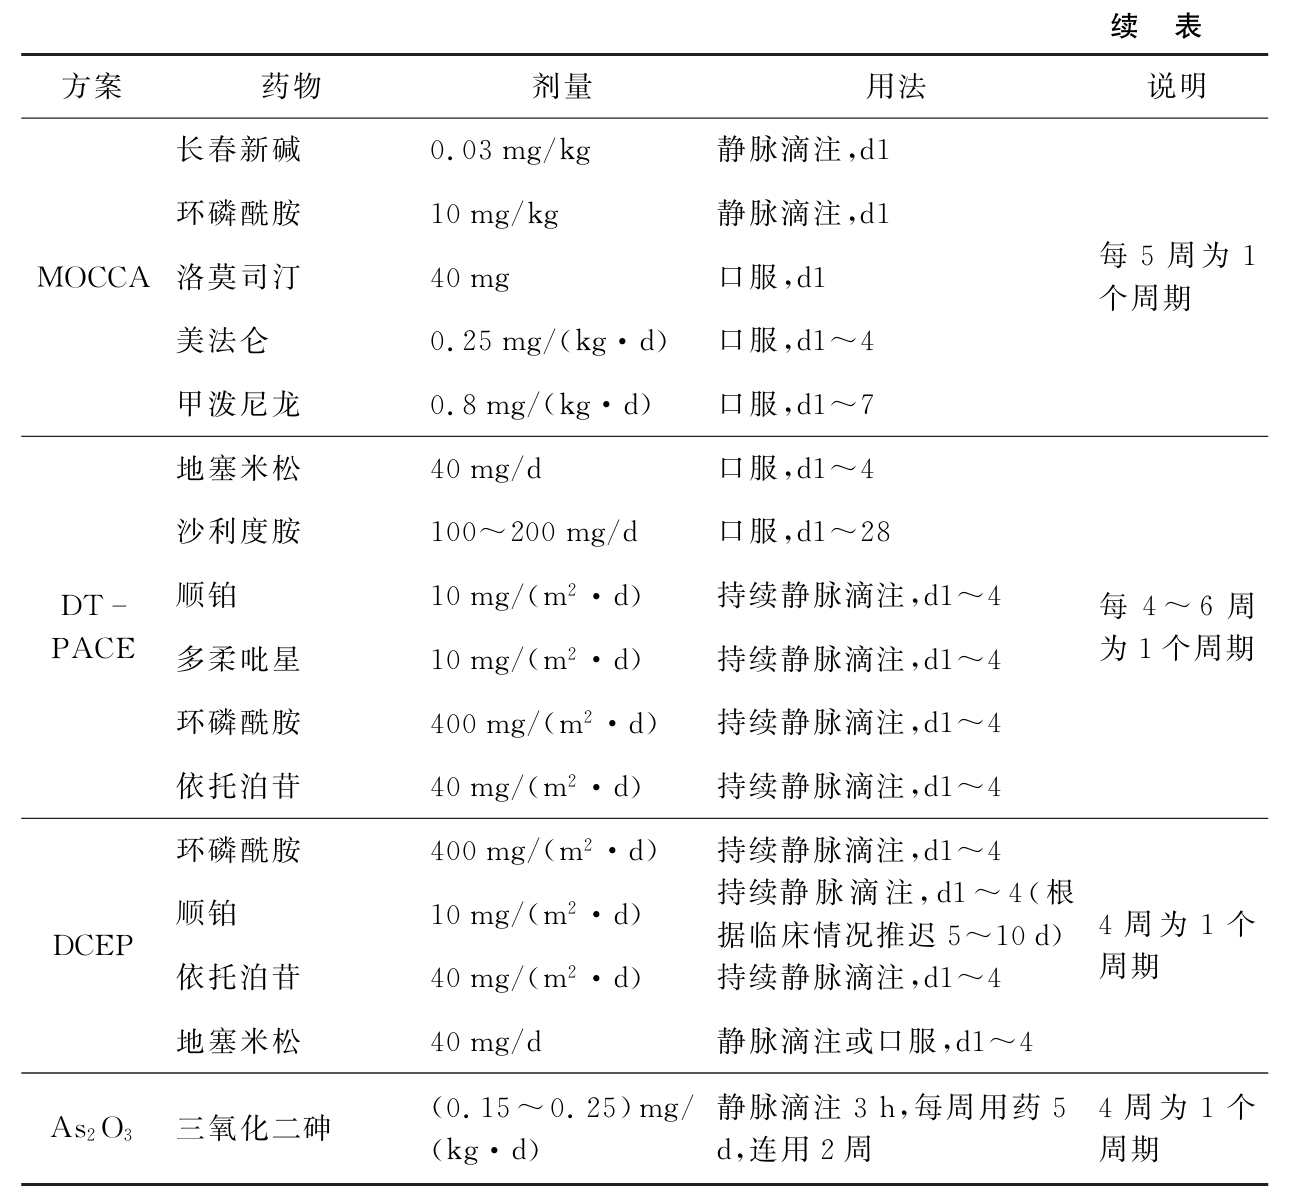
\includegraphics{./images/Image00165.jpg}

6. 辅助治疗

(1)骨病变:对溶骨损害严重可能发生病理性骨折者,应限制活动并配备矫正性支架予以保护;骨折时应予以固定术;有神经压迫如脊椎骨折引起肢体活动不便或截瘫时,有条件可做减张手术,无条件时可行放疗,但可能影响采集足够数量的外周血干细胞和将来的治疗计划,因此较少用。对疼痛患者根据WHO三阶梯止痛原则给予止痛治疗:第一步,对轻度疼痛使用非阿片类镇痛剂;第二步,对中度疼痛使用弱效的阿片药物,可考虑加用非阿片镇痛剂;第三步,对重度疼痛使用强效阿片,或合用非阿片镇痛剂。但是应该避免或非常小心使用非类固醇类消炎药,因为它们对肾脏具有潜在的损害,并能引起胃刺激。有效化疗,特别是含大剂量地塞米松的方案常使骨痛显著改善。

目前研究显示:对于所有有临床症状的骨髓瘤患者,都应接受双膦酸盐治疗,治疗应该至少持续2年。对于Durie-Salmon分期Ⅰ期或Smoldering型的骨髓瘤患者,双膦酸盐治疗的作用尚不明确。

临床应用的双膦酸盐类药物有:①氯屈膦酸钠(clodronate,国内商品名骨膦)为第一代双膦酸盐,氯屈膦酸钠1600mg/d,于晨起空腹口服,服后2小时进餐,可连续服用;或者静滴300mg/d,每个月5日,持续静滴至少2小时。如果肌酐清除率10~30ml/min,剂量减半;如果<10ml/min,忌用。②帕米膦酸钠(APD,阿可达)是第二代双膦酸盐,其强度是氯屈膦酸钠的10倍。帕米膦酸钠90mg,静脉滴注3小时以上,每月1次。如果肾功能不全,输注速度减慢至20mg/h。③第三代双膦酸盐埃本膦酸钠,其活性是APD的100倍,起效快,持续时间长。埃本膦酸钠4mg静脉滴注,每个月1次。每次输注前,检测肌酐,确保水化;如果血清肌酐\textgreater{}265μmol/L,建议不使用。

(2)高钙血症:骨髓瘤中发生有症状的或无症状的高钙血症的患者达到30\%。轻度高钙血症(血钙<3.0mmol/L)无症状,不需紧急处理,但需预防脱水,予以水化,避免使用肾毒性药物;中度高钙血症(血钙3.0~3.5mmol/L),视症状轻重予以正确处理;重度高钙血症(血钙\textgreater{}3.5mmol/L),可迅速导致脱水、肾衰竭及多器官受损表现。需紧急处理:①水化利尿:严重高钙血症常有多尿、脱水,甚至微循环衰竭,首先必须立即补液纠正脱水。补液量视脱水程度和心功能情况而定,一般每日补液3000~4000ml,应首先补给等渗盐水,肾脏排钠增加的同时也增加钙的排出。脱水一旦纠正,可适当应用利尿剂。可静脉推注呋塞米(速尿)40~80mg,必要时2~6小时后重复1次,注意监测电解质;但不能用双氢克尿塞,此药在抑制Na{+}
、Cl{-} 重吸收时也增加了K{+} 、Mg{2+} 的排泄而减少Ca{2+}
和尿酸的排泄。②糖皮质激素:口服泼尼松40~60mg/(m$^2$
·d)或静脉用甲泼尼龙或地塞米松,可通过减少钙从肠道吸收,增加尿钙排出,抑制破骨细胞活性和对肿瘤细胞的直接作用而迅速降低血钙和改善脑病。③双膦酸盐类药物:用法同骨病变。④降钙素抑制骨重吸收和增加肾脏钙的排泄,皮下注射或肌内注射4U/kg,12小时1次,其作用较弱,常与激素合用。⑤化疗:初治或复发MM患者,在处理高钙的同时应尽早化疗。

(3)肾功能损害:预防肾衰竭很重要,去除引起肾功能不全的诱因,如脱水、高尿酸血症、高钙血症、感染尤其是尿路感染;避免使用一切肾毒性药物,如氨基糖苷类、非甾体类抗炎药和造影剂等。水化碱化尿液,至少3000ml/d液体输入,以利于轻链、钙、尿酸和其他有害代谢物的排泄;尽早化疗以减少M蛋白特别是游离轻链的产生;严重肾功能不全应考虑血浆置换,必要时可血透或腹膜透析治疗。

7.
造血干细胞移植治疗 年龄<65岁,全身状态良好的标危MM患者在诱导治疗3~4个疗程后可行自体造血干细胞移植。采用环磷酰胺1.5~4g/m$^2$
联合G-CSF或单独用G-CSF动员方案动员造血干细胞,预处理方案以大剂量美法仑200mg/m$^2$
,老年(超过65~70岁)和肾衰竭患者减量为140mg/m$^2$
。在第1次移植后6个月内进行第二次移植,称为二次移植(顺次移植),二次移植疗效是否优于单次移植目前仍有争议,但仍建议采集造血干细胞时能采集足够两次的量。

高危MM得益自体造血干细胞移植较少,需采用更积极的治疗策略。对于年龄<60岁,全身状态良好,高危患者如有HLA相合同胞供者可采用非清髓性异基因造血干细胞移植。非清髓性异基因造血干细胞移植可以单独应用,或者在自体移植后接着进行。使用常规预处理进行匹配的无关供者移植,其治疗相关死亡率明显高于匹配同胞间移植,目前不被推荐。

【疗效观察与随访】

1.
观察指标 在治疗过程中至少每隔3个月进行1次免疫球蛋白或M蛋白定量,定期检测血常规、肾功能及血钙,血尿游离轻链,每年进行骨髓常规检查及症状评估,视临床需要进行骨髓活检,并考虑PET/CT或MRI。可根据以下疗效标准进行评估。

2. 疗效评估

(1)欧洲血液和骨髓移植小组(EBMT)、国际骨髓移植登记处(IBMTR)和自体血液和骨髓移植登记处(ABMTR)对大剂量治疗和干细胞移植后MM患者反应、复发和进展的标准,见表\ref{tab5-4-6}。

表\ref{tab5-4-6} EBMT/IBMTR/ABMTR反应标准

\begin{longtable}[]{@{}ll@{}}
\toprule
\endhead
& EBMT/IBMTR/ABMTR反应标准\tabularnewline
完全缓解(CR) &
免疫固定电泳检测血清或尿中单克隆M蛋白消失,至少持续6周;骨髓中浆细胞<5\%;溶骨性骨损害大小和数量未增加;软组织浆细胞瘤消失\tabularnewline
部分缓解(PR) &
血清单克隆M蛋白水平下降≥50\%,或尿中游离轻链排出减少90\%或减少到<200mg/24h;不分泌型MM,骨髓浆细胞比例降低≥50\%,以上均至少持续6周{\#}
;溶骨性骨损害大小和数量未增加;软组织浆细胞瘤减小≥50\%(影像学或临床检查)\tabularnewline
轻微缓解(MR) &
血清单克隆M蛋白水平下降25\%~49\%和(或)尿中游离轻链排除减少50\%~89\%,但仍然\textgreater{}200mg/24h,不分泌型MM,骨髓浆细胞比例降低25\%~49\%,持续6周{\#}
;溶骨性病变大小和数量未增加;软组织浆细胞瘤减小25\%~49\%(影像学或临床检查)\tabularnewline
无变化(NC) & 既达不到轻微缓解标准,也无疾病进展\tabularnewline
平台期 &
无持续的骨髓瘤相关的器官或组织损伤(ROTI)持续3个月,M蛋白水平变化或轻链分泌<25\%\tabularnewline
疾病进展(PD) &
\vtop{\hbox{\strut 尽管治疗,骨髓瘤ROTI持续,或在平台期再现}\hbox{\strut ·血清M蛋白水平升高\textgreater{}25\%(\textgreater{}5g/L)和(或)}\hbox{\strut ·尿中M蛋白水平升高\textgreater{}25\%(\textgreater{}200mg/24h)和(或)}\hbox{\strut ·骨髓浆细胞增多\textgreater{}25\%(绝对值增加至少10\%){△}}}\tabularnewline
复发 &
\vtop{\hbox{\strut 既往完全缓解患者的疾病再现,包括免疫固定电泳发现M蛋白}\hbox{\strut ·血清或尿中再次出现M蛋白和(或)}\hbox{\strut ·骨髓中浆细胞和(或)}\hbox{\strut ·出现新的溶骨性病变或软组织浆细胞瘤或原有的骨缺损增大和(或)}\hbox{\strut ·发生不能用其他原因解释的高钙血症}}\tabularnewline
\bottomrule
\end{longtable}

{\#}
仅对于非分泌型骨髓瘤,必须骨髓浆细胞较最初数量减少\textgreater{}50\%(部分缓解),或较最初数量减少25\%~49\%(轻微缓解)。

{△}
在非分泌型骨髓瘤,骨髓浆细胞应该增加\textgreater{}25\%,以及绝对条件至少10\%,MRI检查对于选择性患者也许是有帮助的

(2)国际骨髓瘤工作组统一疗效标准(IMWG标准,2006年),见表\ref{tab5-4-7}。

表\ref{tab5-4-7} 国际骨髓瘤工作组统一疗效标准

\begin{longtable}[]{@{}ll@{}}
\toprule
\endhead
& 国际骨髓瘤工作组统一疗效标准\tabularnewline
严格意义的完全缓解(sCR) &
满足CR标准的同时,具备下列条件:血清游离轻链(FLC)比率正常以及免疫组化、免疫荧光证实骨髓中无单克隆浆细胞\tabularnewline
完全缓解(CR) &
血清和尿免疫固定电泳阴性,无软组织浆细胞瘤及骨髓中浆细胞≤5\%\tabularnewline
非常好的部分缓解(VGPR) &
血清和尿免疫固定电泳阳性,但常规蛋白电泳不能检出M蛋白;或血清M蛋白降低≥90\%及尿M蛋白<100mg/24h\tabularnewline
部分缓解(PR) &
血清M蛋白降低≥50\%,24h尿M蛋白减少≥90\%或降到<200mg/24h;如血尿M蛋白不可测定,则血清受累游离轻链与非受累游离轻链之间的差值缩小≥50\%;如血尿M蛋白及血清FLC均不可测定,并骨髓浆细胞比例≥30\%,则要求骨髓中浆细胞数目下降≥50\%。除了上述标准外,如基线存在软组织浆细胞瘤,则要求浆细胞瘤大小缩小≥50\%\tabularnewline
疾病稳定(SD) & 不符合CR,VGPR,PR及疾病进展标准\tabularnewline
疾病进展(PD) &
满足以下一项:与基线值比较,血M蛋白升高≥25\%(绝对值升高≥5g/L);24h尿M成分升高≥25\%(绝对值升高≥200mg);如血尿M蛋白不可测定,血清受累游离轻链与非受累游离轻链之间的差值升高≥25\%(绝对值升高\textgreater{}10mg/dl);骨髓中浆细胞增多≥25\%(绝对值升高≥10\%);新出现浆细胞瘤、溶骨性病变,或浆细胞瘤增大、溶骨性病变增多;出现与浆细胞增殖相关的高钙血症(校正血钙)\textgreater{}11.5mg/dl(2.65mmol/L)\tabularnewline
临床复发 &
表现为肿瘤负荷增加和(或)出现终末器官功能不全(CRAB)。满足以下一项:出现新的浆细胞瘤或骨质损害;原有浆细胞瘤或骨质损害增加:长径×宽径增加≥50\%(长径、宽径增加至少1cm);高钙血症\textgreater{}11.5mg/dl(2.65mmol/L);Hb降低≥2g/dl(1.25mmol/L);血肌酐升高≥2mg/dl(177mmol/L)\tabularnewline
完全缓解后复发 &
满足以下一项:确认血或尿中M蛋白再次出现;骨髓浆细胞\textgreater{}5\%;发生了新的溶骨性病变或软组织的浆细胞瘤;残留骨骼病变的大小明确增加;出现高钙血症\tabularnewline
\bottomrule
\end{longtable}

【治疗经验与解析】

1.
含有沙利度胺和来那度胺的治疗方案,尤其是同时含有糖皮质激素时,深静脉血栓(DVT)的发生率明显增高。所以在使用这些方案时,要注意DVT的预防。采用的药物包括低分子肝素、华法林或阿司匹林。

2.
硼替佐米的主要不良反应有恶心、呕吐、腹泻、疲劳、周围神经病变及血细胞减少。当患者发生3级非血液学或任何4级血液学的毒性(不包括下面讨论的神经病)时(NCI常见毒性标准),应暂停本品治疗,一旦毒性症状得到缓解,可以重新开始本品的治疗,剂量减少25\%。如果患者发生与本品治疗有关的神经痛或周围感觉神经病,应按以下推荐调整剂量进行治疗:1级,(感觉异常或者反射丧失),不伴有疼痛或者功能丧失,剂量不改变;1级,伴有疼痛或者2级(功能障碍,但不影响日常生活),剂量降至1.0mg/m$^2$
;2级,伴有疼痛或者3级(不影响日常生活)暂停本品的治疗直至毒性缓解后恢复本品的治疗,剂量降至0.7mg/m$^2$
,并且改为每周注射1次;4级(永久的感觉丧失,功能障碍)停止本品的治疗。

3.
地塞米松治疗期间需密切观察血糖、电解质、血压、胃部不适及水肿,以防大剂量激素所致类固醇性糖尿病、高血压、胃炎、消化性溃疡、水钠潴留及低钾血症。糖尿病、高血压患者地塞米松需减量到20mg/d,并需用胰岛素降血糖药物控制血糖及用降血压药物控制血压在正常范围,消化性溃疡、心衰竭患者需慎用。

4.
双膦酸盐类药物常见的副作用包括感冒样症状、胃肠道症状(主要是口服制剂)、眼部副反应、颌骨坏死、贫血、肾功能异常。其中下颌骨坏死和肾损害尤其应引起临床医生的重视。

(1)肾功能损害:发生率9\%~15\%,肾毒性具有剂量和时间依赖性。因此推荐每次使用双膦酸盐前以及在用药过程中需要动态检测肾功能,尤其是在每次给药前要保持水化状态,根据肌酐清除率调整药物剂量。用药过程的监测:对于血清肌酐<265.2μmol/L的患者不需调整剂量;应避免滴注速度过快;建议所有患者均应定期3~6个月监测尿蛋白,如24小时尿蛋白\textgreater{}500mg应考虑停药,直到患者肾功能恢复正常。在双膦酸盐使用过程中尽可能避免或减少使用可能损害肾功能的药物,包括非甾体类抗炎药、沙利度胺、放射线造影剂等。如果不可避免,应在使用双膦酸盐24小时后使用,以避免出现肾衰竭的问题。

(2)下颌骨坏死:目前文献报道长期使用双膦酸盐治疗的多发性骨髓瘤患者的颌骨坏死发生率为1.8\%~12.8\%。使用双膦酸盐过程中应保持口腔卫生,定期口腔检查,尽量避免侵入性的口腔操作,观察患者是否存在口腔溃疡、口腔软组织肿胀以及坏死骨质暴露,当双膦酸盐治疗过程中患者出现牙科问题必须进行牙科手术时,应当尽量保守处理,减少手术操作范围,另外加用抗菌药物有利于预防颌骨坏死的发生。一些研究者推荐在进行口腔侵入性操作前的1~3个月,暂时停用静脉双膦酸盐,当口腔内伤口愈合后再继续双膦酸盐的治疗。

\paragraph{原发性巨球蛋白血症}

原发性巨球蛋白血症又名华氏巨球蛋白血症(WM),以合成和分泌大量单克隆IgM蛋白(巨球蛋白)的淋巴样浆细胞恶性增生、积聚为特点。恶性B细胞在骨髓和髓外浸润以及血中巨球蛋白浓度过高引起一系列的临床症状,患者可表现为全血细胞减少,器官肿大,神经病变,高粘滞综合征。血清中单克隆IgM\textgreater{}10g/L和骨髓中淋巴样浆细胞浸润是诊断本病的必要依据。本病男性多见,多在50岁以上。目前病因尚不明确,约20\%WM患者具有家族遗传性,此外可能与慢性感染及一些肿瘤有关。目前WM仍是一种难以治愈的疾病。

【治疗程序】 如图\ref{fig5-4-5}、图\ref{fig5-4-6}所示。

\begin{figure}[!htbp]
 \centering
 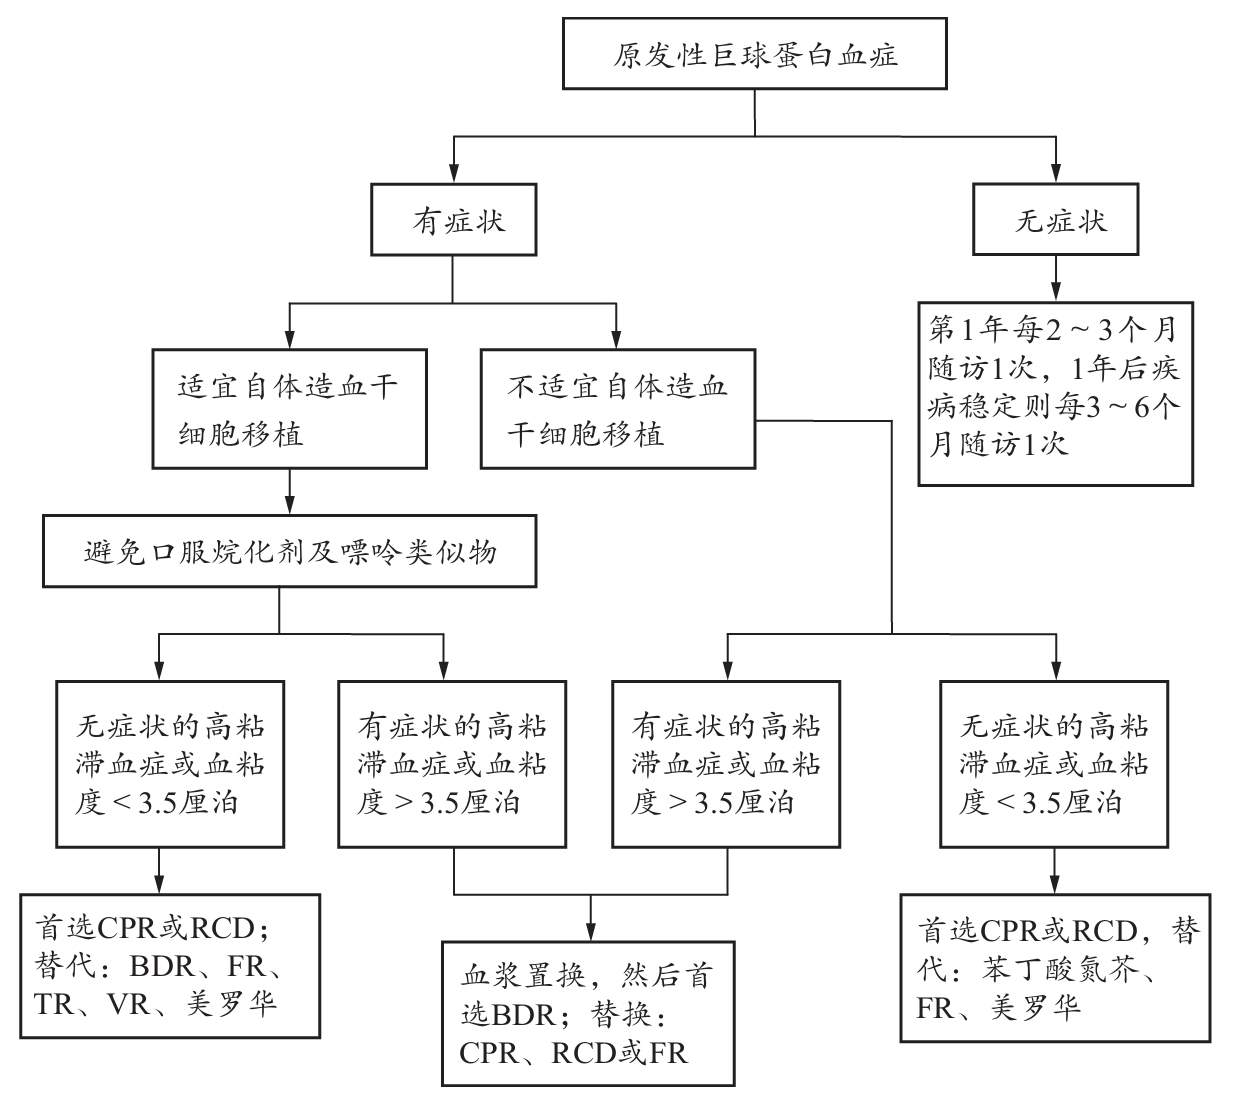
\includegraphics{./images/Image00166.jpg}
 \captionsetup{justification=centering}
 \caption{原发性巨球蛋白血症的治疗程序}
 \label{fig5-4-5}
  \end{figure} 

\begin{figure}[!htbp]
 \centering
 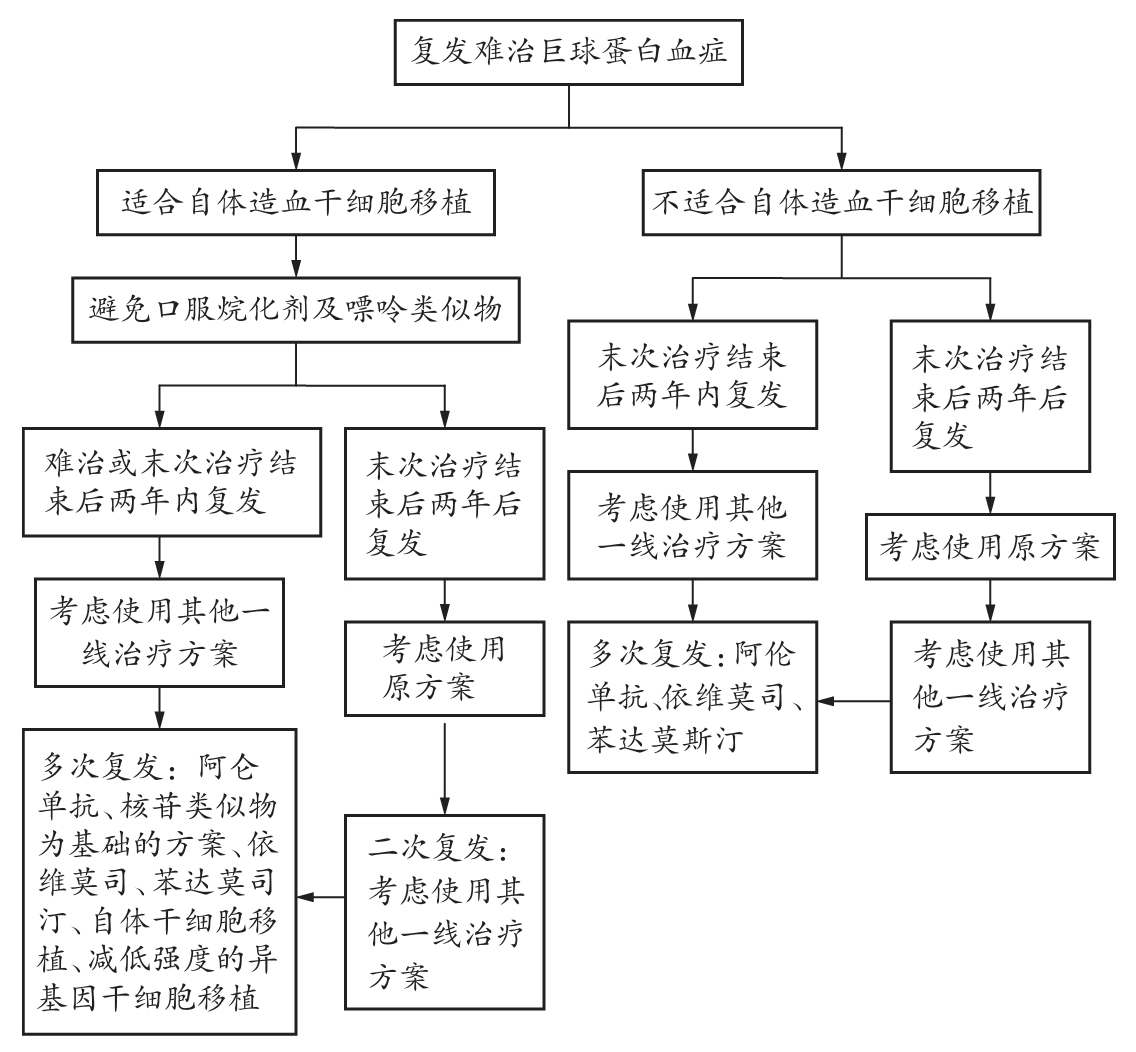
\includegraphics{./images/Image00167.jpg}
 \captionsetup{justification=centering}
 \caption{复发难治巨球蛋白血症的治疗程序}
 \label{fig5-4-6}
  \end{figure} 

【治疗方案】

1.
治疗时机的选择 血红蛋白\textgreater{}120g/L及IgM<30g/L的无症状WM患者呈现惰性病程,常可保持多年稳定而不需治疗,但应严密随访。初始治疗不应单纯基于血清单克隆IgM水平,因为该水平可能与WM的临床表现不相符。开始治疗的指征包括:①高粘滞血症的表现。②贫血、全血细胞减少。③进行性淋巴结肿大和脾肿大。④冷球蛋白血症和神经病变的表现。

2.
一般治疗 积极预防与控制感染;重度贫血可输注红细胞悬液,但应缓慢输入;禁用损害肾功能的药物;对于高粘滞综合征患者,静脉滴注低分子右旋糖酐、丹参等改善微循环,注意改善心脏功能。

3.
血浆置换 由于80\%IgM在血管内,因此血浆置换可去除WM患者血循环中单克隆IgM抗体。单次血浆置换即能有效清除一定量的单克隆IgM,从而降低血粘度,缓解高粘滞血症危象。但IgM抗体浓度下降后,又可反馈性地刺激新的抗体生成。因此,血浆置换后应该联合系统化疗来杀伤恶性增殖的淋巴样浆细胞,以抑制单克隆IgM生成。

4. 化疗

(1)烷化剂:苯丁酸氮芥(瘤可宁)是本病的主要治疗药物,有效率约50\%,既可采用间歇给药,亦可连续给药,效果相似。连续给药每日口服6~12mg,持续2~4周,然后改为维持治疗,每日2~6mg。间歇给药0.7mg/(kg·d),d1或者0.2mg/(kg·d),d1~d4,每21~28日为1疗程。IgM的降低速度较慢,需观察几个月才能确定其疗效。对长期服药患者需注意可能发生骨髓抑制。美法仑和环磷酰胺也可应用,但疗效不如苯丁酸氮芥,环磷酰胺50mg口服每日1~3次,美法仑2mg口服每日1~3次。初治的患者可选用任一种烷化剂口服。

(2)核苷类似物为基础的治疗:氟达拉滨和克拉屈滨治疗WM取得了较好的疗效。对于初发WM,两者的有效率均在70\%以上。氟达拉滨的用法:每日25~30mg/m$^2$
,连续5日静脉滴注,每4周1次。克拉屈滨用法:一般是0.1mg/(kg·d),持续静脉滴注,连用7日或0.12mg/(kg·d)静脉用药2小时,连用5日,间歇期为1个月。对于耐烷化剂的患者,氟达拉滨和克拉屈滨有30\%以上的有效率。氟达拉滨和克拉屈滨的主要不良反应是骨髓抑制和免疫抑制。初治、难治性WM患者均可选用核苷类似物单药治疗。

(3)其他治疗:

1)利妥昔单抗(美罗华):美罗华治疗WM有效,毒副作用小,对于M蛋白\textgreater{}5g/dl,不建议单独应用美罗华,美罗华单独应用后M蛋白会暂时的升高。美罗华以标准剂量375mg/(m$^2$
·w)静脉输注4周,可使30\%~40\%的患者至少获得部分反应。美罗华联合化疗方案主要有:①美罗华可联用氟达拉滨,即FR方案,氟达拉滨的用药方法是每日25~30mg/m$^2$
,连续5日静脉滴注,美罗华第1日用。②R-CHOP方案:美罗华375mg/m$^2$
静脉滴注d1,环磷酰胺750mg/m$^2$ 静脉滴注d1,阿霉素50mg/m$^2$
静脉滴注d1,长春新碱1.4mg/m$^2$
(最大不超过2mg),泼尼松100mg/d,d1~d5。③CPR方案:美罗华375mg/m$^2$
静脉滴注d1,环磷酰胺1000mg/m$^2$
静脉滴注d1,泼尼松100mg/d,d1~d5。④美罗华合用环磷酰胺和地塞米松(RCD方案),地塞米松20mg,静脉滴注,d1,紧接着予以美罗华375mg/m$^2$
静脉滴注d1,环磷酰胺100mg/m$^2$
口服,每日2次,d1~d5,21日为1个疗程,共6个月。以上方案可用于初治、难治性WM患者。美罗华与骨髓抑制无关,对干细胞也无毒性作用,因此对已有或有发展为血细胞减少趋势的患者以及准备接受干细胞采集和经大剂量化疗的患者均是合适的选择。

2)沙利度胺:沙利度胺治疗WM的确切疗效尚需要大样本、随机、对照研究证实。沙利度胺治疗WM的临床试验中,初始剂量为200mg/d,逐渐增加剂量,最大用至600mg/d。目前尚有采用TR方案的小样本Ⅱ期临床试验:沙利度胺200mg/d,2周,后改为400mg/d,50周,美罗华每周375mg/m$^2$
静脉滴注,第2~5周,第13~16周,总反应率为70\%。

3)蛋白酶体抑制剂:硼替佐米目前已成功用于WM患者的治疗,取得很好的临床疗效。初治、难治性WM患者均可选用含硼替佐米的方案:硼替佐米联合地塞米松、美罗华组成BDR方案,具体为:硼替佐米:1.3mg/m$^2$
静脉注射,d1,4,8,11,21日为1疗程,地塞米松40mg静脉滴注,d1,4,8,11,美罗华375mg/m$^2$
静脉滴注,d11。硼替佐米和美罗华组成VR方案,具体为:硼替佐米1.6mg/m$^2$
静脉注射,d1,8,15,每28日为1个疗程×6周期,美罗华375mg/m$^2$
静脉滴注,每周1次,第1和第4周期。

4)其他新药:①阿仑单抗:这是一种单克隆抗体,可与WM肿瘤细胞表面的CD52抗原结合,目前临床试验正在进行中。②CD22单抗:这是近几年用于治疗WM的一种新型单抗。一般用量每次360mg/m$^2$
,每周1次,共4次。它与其他药物联合使用获得很好的临床疗效。优点是患者耐受性好,无剂量限制毒性,无骨髓抑制。③依维莫司(Everolimus,RAD001):是口服的mTOR信号通路抑制剂,Ⅱ期临床试验显示复发、难治WM患者总反应率是70\%,其中44\%达到主要反应,28\%获得轻微反应。用法:10mg/d,根据毒副反应可降低至5mg/d。

(4)造血干细胞移植治疗:自体干细胞移植治疗WM的资料有限,其原因在于WM患者年龄多大于70岁。自体干细胞移植治疗可作为挽救治疗方案用于年轻的多次复发和原发耐药的WM患者。非清髓异基因干细胞移植治疗WM的例数更少,相关病死率高,但完全缓解率明显高于自体移植,故适用于较年轻有供者来源的患者。清髓性的异基因造血干细胞移植因移植相关死亡率高,一般不予考虑。

【疗效观察与随访】

1. 观察指标

(1)症状、体征:观察淋巴结、脾肿大缓解情况,神经病变缓解情况,高粘滞血症和冷球蛋白血症的改善情况,全身情况,如发热、盗汗、乏力的改善情况。

(2)实验室检查:随访血常规,肾功能,免疫球蛋白定量,免疫固定电泳,肝功能,血粘度,骨髓,血尿轻链,C-反应蛋白,β{2}
-微球蛋白等。

2. 疗效标准

(1)完全缓解:相隔6周两次免疫固定电泳血清中单克隆M蛋白成分消失,IgM定量正常,淋巴结肿大/脏器肿大消失,体格检查、骨髓象及血清粘滞度均恢复正常。

(2)部分缓解:血清蛋白电泳单克隆IgM减少50\%以上,体检或CT扫描淋巴结肿大或脏器肿大缩小50\%以上,无活动性病变的新的症状和体征。

(3)轻微缓解:血清蛋白电泳单克隆IgM减少在25\%以上但在50\%以下,无活动性病变的新的症状和体征。

(4)进展:血清中M蛋白增加25\%。

(5)疾病稳定:血清蛋白电泳单克隆IgM减少和增高均<25\%,淋巴结肿大或脏器肿大、血细胞减少、临床与疾病相关的症状、体征等无进展。

(6)疾病进展:2次检测证实血清蛋白电泳单克隆IgM增高\textgreater{}25\%,或者发现淋巴结肿大或脏器肿大、贫血、白细胞减少、血小板减少有进展,或出现与疾病相关的症状:持续发热\textgreater{}38.4℃、盗汗、体重下降\textgreater{}10\%、神经病变,高粘滞综合征、症状性冷球蛋白血症和淀粉样变。

3.
随访 注意病情变化,观察症状、体征变化,避免合并症。每两个疗程检测血常规、血清蛋白电泳、免疫球蛋白定量,既往有脏器肿大者3~6个月予以CT扫描,有症状者予以血粘度检测。

【治疗经验与解析】

1.
目前WM治疗有效的方案较多,但很少有比较性的临床试验研究,尚无证据表明哪种药物、哪种方法更为有效。基于专家的共识推荐,烷化剂、核苷酸类似物和美罗华都可作为WM一线治疗的选择。在选择化疗药物时需考虑如下诸多因素:①患者年龄;②明显的脾肿大和淋巴结肿大,血细胞减少(特别是血小板减少);③是否适合自体干细胞移植;④症状严重需要及时控制;⑤是否有高粘滞血症;⑥周围神经病;⑦可能同时合并的其他疾病。最近有学者报道在初治的WM患者中,应用RCD方案治疗,有效率达83\%,其中完全缓解率7\%,部分缓解率67\%,9\%微小缓解。2年的无进展生存率90\%,只有9\%的患者有3或4级的血液学毒性。但目前仍没有随机临床试验证明RCD方案优于核苷类似物或蛋白酶体抑制剂为基础的方案。有高粘滞血症症状和体征的患者,血浆置换应先于系统化疗,年轻患者或合并其他严重并发症患者需立即纠正的可考虑氟达拉滨,对于无严重并发症的老年患者可选用烷化剂;血清β{2}
-微球蛋白升高及重度贫血的年轻患者可考虑大剂量化疗联合自体干细胞移植;如患者合并严重的神经症状,应慎用硼替佐米;不适合予大剂量化疗的患者,三种药物可任选其一,但是当疾病需迅速控制时,应首选氟达拉滨或克拉屈滨;对于血细胞减少的患者,建议用美罗华,而对于M蛋白\textgreater{}5g/dl,不建议单独应用美罗华;对某一药物治疗后复发或难治的病例可换用其他的一线用药。

2.
WM细胞表达CD20,因此可应用CD20单抗美罗华治疗,初始治疗应用美罗华可改善血细胞减少,神经病变和骨髓浸润等症状。在初治和既往治疗过的WM患者中,美罗华的缓解率为29\%~65\%。一些患者应用美罗华后单克隆蛋白可出现反常的升高,升高水平可持续达4个月,这并不表示治疗失败。目前尚没有比较美罗华和其他治疗的随机临床试验,因此不能认为美罗华优于其他治疗。对于低危的WM的患者,或是有IgM相关的神经病变并需要治疗,或是激素治疗无效的溶血性贫血,可用美罗华单药治疗。目前没有证实WM患者美罗华维持治疗可以改善至进展时间,因此不推荐维持治疗。在美罗华使用过程中的主要副作用有发热、寒战、皮疹和恶心呕吐,以及喉头水肿、低血压、休克及死亡。因此用前30分钟应口服或肌内注射非那根25mg和静脉注射地塞米松5~10mg。

3.
目前尚没有临床试验证明最优的治疗选择。挽救治疗的选择依赖于初始治疗方案,初始治疗缓解的质量和持续时间,还有一些其他因素,如对初始治疗的耐受性和是否预备行干细胞移植治疗,第四届WM国际工作组的专家共识推荐如果患者缓解的时间长,可以重新应用一线治疗的方案,如果患者缓解时间过短或是对一线治疗耐药,推荐应用与一线治疗药物不同类的药物治疗。专家共识中强调了复发患者中应用氟达拉滨,硼替佐米和阿伦单抗,单独应用或与美罗华联合可能有效。自体或是异基因干细胞移植也可以考虑。最近有研究表明苯达莫司汀单药或是联合美罗华可作为复发患者的有效治疗方案(图\ref{fig5-4-7})。

\begin{figure}[!htbp]
 \centering
 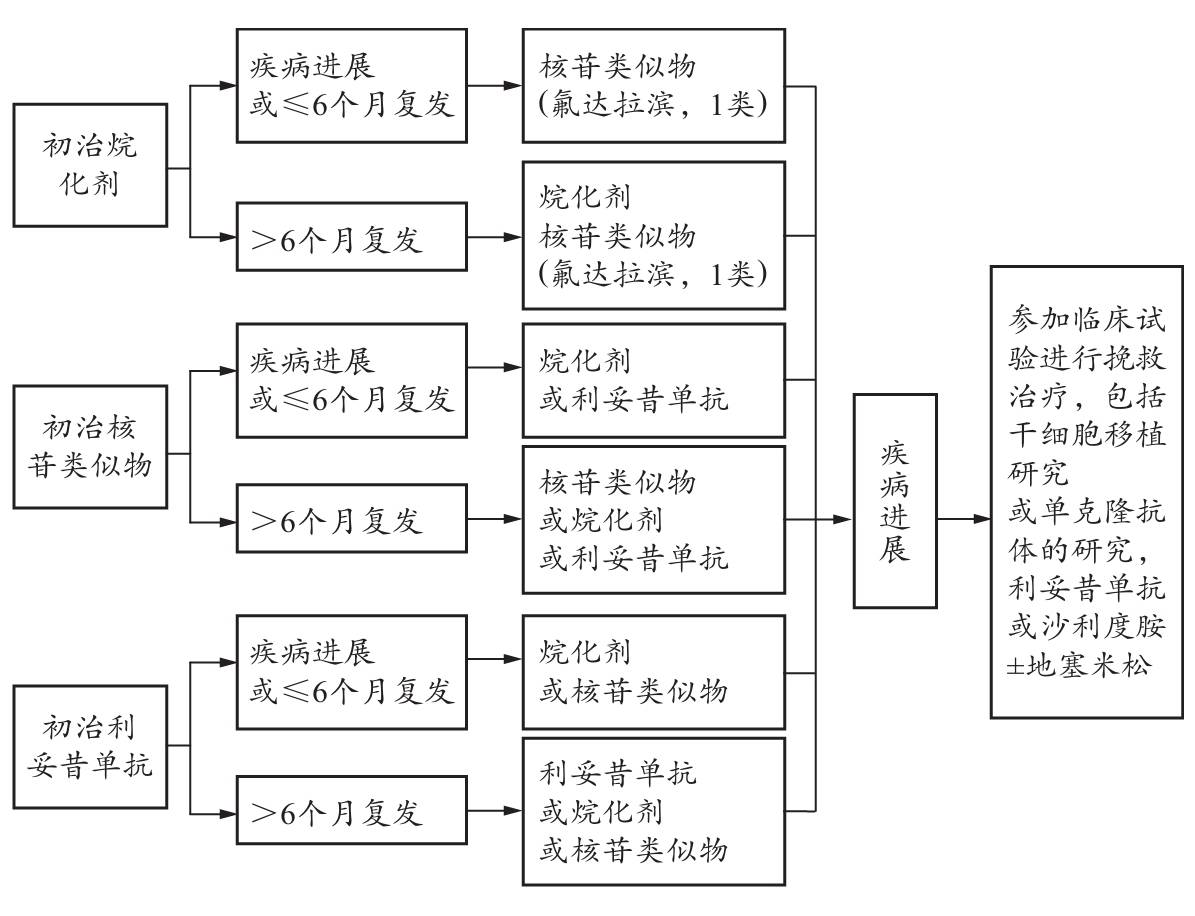
\includegraphics{./images/Image00168.jpg}
 \captionsetup{justification=centering}
 \caption{复发性巨球蛋白血症的治疗流程}
 \label{fig5-4-7}
  \end{figure} 

疾病进展:定义为血清或尿M蛋白持续升高25\%,腺体增大或器官增大。

疾病部分缓解:定义为各种可测量的疾病指标减少50\%,并≥4周后再次测量证实。

4.
关于切脾治疗 切脾治疗仅见个例和小样本病例报道,对常规化疗失败的WM患者行脾切除可获得一定效果,然而,巨脾在WM中很罕见,切脾的疗效有待进一步证实。

(屈晓燕 费小明 朱华渊 陈丽娟 李建勇 许家仁)

\paragraph{重链病}

重链病(HCD)是一组特殊的B淋巴细胞及浆细胞克隆增生性疾病,其特征是克隆增生的恶性细胞合成和分泌大量结构均一的不完全免疫球蛋白,该蛋白质仅由不能与轻链结合的异常重链组成,并且克隆增生的细胞可以同时分泌游离轻链或者不表达轻链。现已发现γ、α、μ和δ四种类型HCD,δHCD仅见个案报道。其临床表现随类型不同表现各异。重链病的病因尚不清楚,感染、自身免疫病及免疫球蛋白合成缺陷与其发病有密切关系。

【治疗方案】

1.
γ-HCD 目前尚无满意的治疗方案。部分患者可以不经特殊治疗而有一个较长的临床过程。对有症状并伴低度淋巴样浆细胞增生的患者可用苯丁酸氮芥治疗,而对进行性加重的患者可选用COP,CHOP或MP方案,除个别病例可达完全缓解外,疗效均不满意。近年来有报道采用氟达拉滨、美罗华治疗有效。放射治疗在缩小肿大淋巴结和脾脏以消除压迫症状方面是有效的,但易于复发。

2.
α-HCD 依据疾病严重程度及病理分期不同,治疗方法不同。A期可选用抗生素治疗,如口服罗红霉素、甲硝唑、氨苄西林等,尽量清除肠道内的细菌和寄生虫。对于口服抗生素疗效差或疾病已处于B、C期的患者,应采用抗肿瘤化学治疗,通常选择非霍奇金淋巴瘤的方案,如COP、CHOP等,也可采用全腹放射治疗(包括肝、肾),疗效不如化疗。对于年轻的有条件的难治复发患者可考虑干细胞移植。

3.
μ-HCD 目前尚无特殊的治疗手段,主要针对内在的B细胞淋巴瘤增生性疾病如慢性淋巴细胞白血病的治疗。

【疗效观察与随访】

1. 观察指标 常见症状与体征、血常规、淋巴结活检等。

2. 疗效评估 本病预后差,应重点注意防治感染,合理选用抗生素。

3. 随访 密切观察病情变化,积极防治并发症。

【治疗经验与解析】

1.
本病本质上是一些少见的淋巴瘤亚型,如γ-HCD为淋巴浆细胞淋巴瘤变异型,α-HCD为结外粘膜相关淋巴组织淋巴瘤的亚型,μ-HCD则为CLL变异型。本病尚无特别而有效的方法,治疗主要参照淋巴瘤治疗的方案。

2.
α-HCD的病程长短不一,主要取决于病理分期,通常疾病发展较缓慢。经治疗的患者5年平均生存率67\%。γ-HCD多数患者在数月内死于感染和疾病的进展,亦有患者发展为浆细胞白血病而死亡,存活5年以上者少见。部分患者可存活5年以上,甚至重链蛋白消失。μ-HCD预后差,病程为1个月至11年,中位生存期24个月。

(屈晓燕 费小明 王莉 陈丽娟 李建勇 许家仁)

\paragraph{淀粉样变性}

淀粉样变性是一组疾病,此组疾病的特点是因蛋白质代谢紊乱产生的特殊淀粉样蛋白质沉积到一处或多处器官组织细胞间,造成组织器官结构和功能改变,从而导致相应的临床表现的异质性疾病。临床上淀粉样变性可分为系统性和非系统性两大类,也可分成原发性和继发性。原发性系统性淀粉样变性是淀粉样变性中最常见的类型,约占所有淀粉样变性的70\%。根据淀粉样蛋白性质,淀粉样变可分为:①AL型淀粉样变性,②AA型淀粉样变性,③β2-MG型淀粉样变性,④遗传性淀粉样变性,⑤AH型淀粉样变性。

【治疗方案】 目前尚无充分的数据确定最佳治疗选择,如可能所有患者尽可能加入临床试验。治疗应针对三方面:①降低淀粉样物质产生;②抑制淀粉样物质的聚集和沉积;③促进已沉积的淀粉样物质的溶解。迄今尚无特异性消除淀粉样物质沉积灶的方法,治疗的重点是根据淀粉样蛋白的种类,选择合适的治疗方法减少淀粉样前体蛋白,合理的治疗计划应包括:

1. 控制原发病,加强病因治疗。

2. 根据淀粉样蛋白的种类,降低淀粉样物质产生。

(1)AL型淀粉样变可选用化疗:

1)MD方案:美法仑10mg/(m$^2$
·d),口服,d1~d4,地塞米松40mg/d,口服,d1~d4,每月1次,持续治疗12~18个疗程,12个疗程后血清或尿中淀粉样蛋白减少50\%以上可停止治疗。

2)VAD方案:长春新碱0.4mg/d,持续静脉滴注4日,多柔比星9mg/(m$^2$
·d),持续静脉滴注4日,地塞米松(Dex)40mg/d,口服d1~d4、d9~d12、d17~d20。每4周重复给药。

3)新药治疗:沙利度胺+地塞米松(TD方案):沙利度胺100~200mg/d,口服,每晚1次,地塞米松40mg/d,分1~2次口服,d1~d4(偶数周期),d1~d4,d9~d12,d17~d20(奇数周期)。环磷酰胺+沙利度胺+地塞米松(CTD):复方环磷酰胺500mg,口服,d1,8,15,沙利度胺200mg/d,口服,每晚1次,地塞米松40mg/d,口服,d1~d4,d9~d12,21日为1个疗程,患者耐受性好可用至12个疗程。来那度胺+地塞米松(LD方案):来那度胺25mg/d,口服,d1~d21,地塞米松40mg/d,口服,d1~d4,d15~d18,28日为1个疗程,最多可用12个疗程。硼替佐米+地塞米松(BD方案):硼替佐米1.3mg(m$^2$
·d),静脉注射,d1,d4,d8,d11,地塞米松40mg/d,口服或静脉滴注,d1~d4,每21日为1个疗程,共用6个疗程。

(2)干细胞移植治疗:为了减少动员过程的危险性,动员时应给予小剂量G-CSF[10~12μg/(kg·d)],分2次皮下注射,连续给药5日,在第5日早晨给予G-CSF2~4h后开始采集。预处理采用中高剂量美法仑:美法仑片剂140或200mg/m$^2$
,顿服,d-2,或美法仑注射剂140或200mg/m$^2$
,静脉滴注(每支50mg,每支静注时间不少于15min)d-2,于d0输注自体造血干细胞。适用于AL型淀粉样变选用。

(3)家族性地中海热、溃疡性结肠炎、强直性脊柱炎和类风湿关节炎合并淀粉样变性:秋水仙碱0.6mg,口服,每日3次,至症状缓解或出现副作用。继发于青少年慢性多关节炎的肾淀粉样变:苯丁酸氮芥(瘤可宁)0.1~0.2mg/(kg·d),分1~3次餐后口服,4~8周为1个疗程,连用3~12个月。

3. 消除淀粉样沉积灶 目前尚无特效方法。

4.
对症支持治疗 可以推迟靶器官的功能衰竭、提高生活质量、延长生存期;禁用钙通道阻滞剂,肾功能不全者可予以血液透析或腹膜透析治疗,AA型淀粉样变性患者进行肾移植;心脏淀粉样变性患者进行心脏移植;家族性淀粉样变性多神经病患者可行肝脏移植。

【疗效观察与随访】

1.
观察指标 观察心功能的情况,有无神经病变,注意舌有无淀粉样物质沉积,胃肠道功能等。观察血常规,肝功能,肾功能,骨髓检查,血清和尿免疫球蛋白定量,心电图,超声心动图,血尿轻链。

2. 疗效评估 好转标准:症状减轻,相关检测指标改善。

3.
随访 注意观察病情,观察症状、体征变化,避免并发症,定期复查相关检测指标。

【治疗经验与解析】

1.
需严格把握化疗的适应证。抗肿瘤坏死因子治疗被认为是治疗继发于类风湿性关节炎的AA型肾淀粉样变的一种有效疗法,etanercept作为肿瘤坏死因子阻滞剂,已被证实能延缓AA型肾淀粉样变患者肾功能的恶化,同时能抑制类风湿性关节炎患者的炎症反应。最近一个小分子新药eprodisate已开始应用于临床,可以抑制淀粉样纤维形成,证实可减缓AA型淀粉样变患者的肾功能下降速度。二氟尼柳和tafamidis用于治疗遗传性及老年性系统性淀粉样变性的临床试验正在进行中。

2.
关于移植,由于淀粉样变性患者通常有肾、心脏、肝脏、胃肠道或神经病变,故其移植相关死亡率高于MM患者。对AL淀粉样变累及心脏或多脏器者移植相关死亡率可高达38\%以上,因此患者的选择是移植成功与否的一个重要因素。推荐的入选标准包括疾病有症状、无多发性骨髓瘤、年龄小于70岁、心脏室间隔厚度小于15mm、左室射血分数大于55\%、血肌酐小于20mg/L、碱性磷酸酶不超过正常值的3倍、直接胆红素小于20mg/L。

(屈晓燕 费小明 洪鸣 陈丽娟 李建勇 许家仁)

\paragraph{POEMS综合征}

POEMS综合征是一种与浆细胞病有关的多系统病变,临床上以多发性周围神经病(polyneuropathy)、脏器肿大(organomegaly)、内分泌障碍(endocrinopathy)、M蛋白血症(M-protein)和皮肤病变(skin
change)为特征,取其英文首字母组成POEMS综合征。除了以上临床特点外,患者还可表现为硬化性骨损害,Castleman病,视乳头水肿,水肿等表现。

【治疗方案】

1.
放疗 局部区域的单个或多个骨硬化性损害可采用放疗。如果患者出现广泛的骨硬化性损害或骨髓浆细胞增多,需进行全身治疗。孤立性浆细胞瘤可给予40~50Gy剂量的放疗。非神经病变的表现,如色素沉着、水肿、多毛、男性乳腺发育和肝脾肿大相对神经病变改善迅速。

2. 系统性治疗

(1)美法仑联合泼尼松治疗对约40\%的POEMS综合征患者有效。最佳的治疗持续时间尚未确定,借鉴多发性骨髓瘤(MM)的治疗,可进行12~24个月的治疗。具体为:美法仑8mg/(m$^2$
·d)分2~3次口服,d1~d4,泼尼松60mg/(m$^2$
·d)分2~3次口服,d1~d4,每4~6周重复。

(2)尚没有前瞻性研究支持皮质类固醇用于治疗POEMS综合征,但是个案报道表明皮质类固醇治疗有效。

(3)采用沙利度胺、来那度胺及硼替佐米等新药治疗POEMS综合征的经验尚少。由于沙利度胺或来那度胺具有抗-VEGF及抗-TNF作用,因此理论上可用其治疗本病。具体治疗方案:沙利度胺+地塞米松(TD方案):沙利度胺(100~200)mg/d,口服,每晚1次,地塞米松40mg/d,分1~2次口服,d1~d4(偶数周期),d1~d4,d9~d12,d17~d20(奇数周期)。来那度胺+地塞米松(RD方案):来那度胺25mg/d,口服,每日1次,d1~d21,地塞米松40mg/d,分1次~2次口服,d1~d4,d9~d12,d17~d20,4疗程后d1~d4。硼替佐米联合地塞米松(BD方案):硼替佐米1.3mg/m$^2$
,静脉注射,d1,d4,d8,d11,21日为1个疗程,地塞米松40mg静脉滴注,d1~d2,d4~d5,d8~d9,d11~d12。

(4)国外学者报道贝伐单抗治疗POEMS综合征患者改善了患者的神经病变、水肿和呼吸道症状,而一些患者发生了毛细血管渗漏综合征。

(5)大剂量化疗联合自体外周血干细胞移植是POEMS综合征患者一种新兴的治疗方法。首例采用该方法的报道来自于一例25岁的女性POEMS综合征患者,该患者采用大剂量化疗继之以骨髓移植,移植63日后患者死于多器官衰竭。国外文献报道的接受自体外周血干细胞移植的POEMS综合征患者38例,随着时间的推移,所有患者神经病变得到改善。自体外周血干细胞移植后其他一些临床症状也得到缓解,包括一些患者的血管内皮生长因子(VEGF)水平。

【疗效观察与随访】

1. 观察指标

(1)症状、体征:观察患者周围神经病变的缓解情况,器官肿大的缓解情况,内分泌病变的改善情况,皮肤病变的缓解情况等。

(2)实验室检查:监测血常规,血清和尿免疫球蛋白,骨髓情况,内分泌功能等。

2.
疗效评估 缓解标准:症状、体征减轻,相关检测指标改善,病情稳定3个月以上。

3.
随访 注意病情观察,观察症状、体征等变化,避免并发症,定期复查相关检测指标。

【治疗经验与解析】

1. 目前没有POEMS患者的随机对照临床试验,都是基于回顾性研究。

2.
关于新药治疗POEMS综合征,目前,采用沙利度胺、来那度胺和硼替佐米等新药治疗的经验尚少。采用沙利度胺治疗时,应注意以下问题:①MM患者接受沙利度胺治疗后,约20\%的患者可出现周围神经病变;②沙利度胺在原发性系统性淀粉样变病患者中可导致水钠潴留;③作为单一治疗药物,沙利度胺对于浆细胞病的疗效并不优于口服烷化剂治疗。来那度胺的神经毒性较轻,该药物可用于治疗POEMS综合征。采用硼替佐米治疗POEMS综合征患者时可能加重神经病变。

3.
其他治疗方法包括静脉用丙种球蛋白、血浆去除术、干扰素α、硫唑嘌呤、环孢素A和全反式维甲酸。国外有学者认为这些治疗疗效不大,但这些治疗通常与糖皮质激素或放疗联用,因此比较难评估这些治疗的作用。POEMS综合征与慢性炎症性脱髓鞘性多神经病不同,血浆去除术和静脉注射免疫球蛋白临床疗效不佳。

4.
烷化剂治疗过程中应定期检测外周血象,并根据血象及时调整剂量,以免发生不可逆的骨髓抑制。预备行自体干细胞移植的患者在采集干细胞前应避免应用烷化剂,以免影响干细胞采集。

5.
国外学者报道POEMS综合征患者干细胞移植相关的死亡率高于MM患者。超过1/3的患者需要机械通气。综合已发表的移植后POEMS患者数据,死亡率为7.4\%。

(屈晓燕 费小明 陈丽娟 李建勇 许家仁)

\section{止血和血栓}

\subsection{血管性紫癜}

血管性紫癜是一组血管壁异常导致的出血性疾病。本组疾病的共同特征表现为自发性皮肤瘀点和瘀斑。按照疾病的原因可以分为原发性和继发性两大类。

\paragraph{过敏性紫癜}

过敏性紫癜(AP)是机体对某些致敏原发生变态反应,导致毛细血管壁通透性和脆性增加,伴发小血管炎,其本质是一种血管变态反应性出血性疾病,是血管性紫癜中最常见的类型,又称Schonlein-Henoch综合征。本病好发于儿童和青少年,平均年龄为5~7岁。根据不同的临床表现分为皮肤型、关节型、腹型、肾型和混合型。

【治疗方案】

1.
一般治疗 去除可能存在的致敏原;治疗上呼吸道感染,清除局部病灶如扁桃体炎,祛除肠道寄生虫等。

2. 药物治疗

(1)一般药物治疗:

1)抗组胺类药物:可选用H{1}
受体阻滞剂口服,如马来酸氯苯那敏(扑尔敏)4~8mg,口服,每日1次或氯雷他定(开瑞坦)10mg,口服,每日1次。

2)止血药物:卡巴克洛(安络血)、酚磺乙胺(止血敏)等,如止血敏3~5g静滴。

3)辅助治疗:包括芦丁、维生素C和钙剂等,如10\%葡萄糖酸钙10~20ml静脉滴注或维生素C
2~5g,复方芦丁片20~40mg,口服,每日3次。

(2)其他药物治疗:

1)糖皮质激素:抑制抗原抗体反应,改善毛细血管通透性,对皮肤型、腹型、关节型紫癜效果较好。但对肾型紫癜效果欠佳,不能改变肾型患者预后,也不能防止复发。如泼尼松30mg/d,口服,如1周后皮疹不退可加至40~60mg/d,紫癜消失后每周减少日服量10mg,直至减完。

2)免疫抑制剂:对于激素无效或者较为严重患者可选用环磷酰胺、硫唑嘌呤、环孢素A等免疫抑制剂。一般适用于糖皮质激素治疗效果不佳,特别是伴有肾损害的病例。如环磷酰胺2~3mg/(kg·d),口服,每日3次,连用4~6个月。

3.
对症治疗 关节症状明显者,可酌情应用水杨酸类如阿司匹林,但需注意其抑制血小板功能的副作用。腹痛明显者,可给予山莨菪碱。消化道出血应给予止血治疗,必要时输血。紫癜性肾炎治疗根据肾脏受累程度不同而异,建议肾内科诊治。

【疗效观察与随访】

1.
观察指标 常见症状与体征、紫癜分布、范围、类型、血常规、血小板、尿常规等。

2. 治愈标准 紫癜消退,症状消失,近期内无新的紫癜出现。

3.
随访 注意病情观察,观察症状和体征等变化,并且注意避免诱发因素,找出过敏原。

\paragraph{遗传性出血性毛细血管扩张症}

遗传性出血性毛细血管扩张症(HHT)是一种常染色体显性遗传性血管异常疾病,以皮肤、粘膜多部位毛细血管扩张和扭曲为特征。其发病机制是位于9号染色体endoglin基因(HHT1)或12号染色体的ALK1基因(HHT2)发生异常,受累的血管脆弱易破而发生出血。

【治疗方案】 由于本病系遗传性疾病因此无特效治疗,对于无明显临床症状患者可随访观察,出现较为明显出血的患者临床处理原则以对症和支持治疗为主。

1.
对症治疗 出血时主要局部止血为主。如鼻出血可用吸收性明胶海绵或其他鼻腔填塞物加压止血处理,可同时加用止血剂如:酚磺乙胺(止血敏)0.25~0.75g,肌内注射或稀释后静脉滴注,每日1~2次。

2.
手术治疗 反复发生鼻出血者在上述治疗无效时可采用激光凝固、冷冻、手术缝合等措施,但易于复发。

【疗效观察与随访】

1. 观察指标 主要观察局部出血相关的症状和体征。

2. 疗效评估 缓解:出血停止、血压稳定。

3. 随访 注意观察出血情况。

【治疗经验与解析】 本病为遗传性疾病,主要以对症与支持治疗为主,积极防治出血。应避免外伤,避免服用阿司匹林类药物,避免能引起血压增高、血容量增加及血管扩张的因素和药物。

\paragraph{单纯性紫癜}

单纯性紫癜是指无其他病因,自发或轻微外伤导致的皮肤尤其双下肢反复出现紫癜,不经治疗可以自行消退的一种出血性疾病。本病发病以年轻女性为主,月经期、青春期好发,一般不出现内脏等重要器官的出血。

【治疗方案】 单纯性紫癜临床多表现为机体在无明显诱因或者轻微外伤后四肢出现紫癜,大多数不经过治疗可以自行消退,本病常在一个家庭内出现多例类似患者,部分病例表现为遗传性的单纯性紫癜,系染色体显性遗传。治疗方面主要是避免可能存在的外伤,大多数患者无需特殊药物治疗和处理紫癜可以自行消退,同时避免使用对于血管壁和血小板有影响的药物。

1. 单纯性紫癜大多数可以自行消退,无需特殊治疗和处理。

2.
如果紫癜症状较为明显,可以使用维生素C、芦丁和安络血等增加血管稳定性、减少渗出的药物进行对症处理。具体为芦丁20~40mg,口服,每日3次;安络血2.5~5mg,口服,每日3次。

3. 尽量避免使用阿司匹林等影响血小板功能的药物。

【疗效观察与随访】 大多数单纯性紫癜患者疾病呈自限性和良性过程,虽然有可能反复发生,但是即使在外伤、外科手术等应激状态时并不会发生过度出血的危险。

【治疗经验与解析】 本病确诊需要建立在排除其他原因造成皮肤紫癜的前提下,因此需要和其他病因造成的紫癜相鉴别。

\subsection{血小板疾病}

\paragraph{原发免疫性血小板减少症}

原发免疫性血小板减少症(ITP),既往称为特发性血小板减少性紫癜,是临床上最常见的血小板减少性疾病。大多数该病患者体内可检出针对自身血小板的自身抗体,目前认为ITP系机体免疫功能异常所致。本病的发生率为5~10/10万人口,女性略多于男性。

【治疗程序】 如图\ref{fig5-5-1}所示。

\begin{figure}[!htbp]
 \centering
 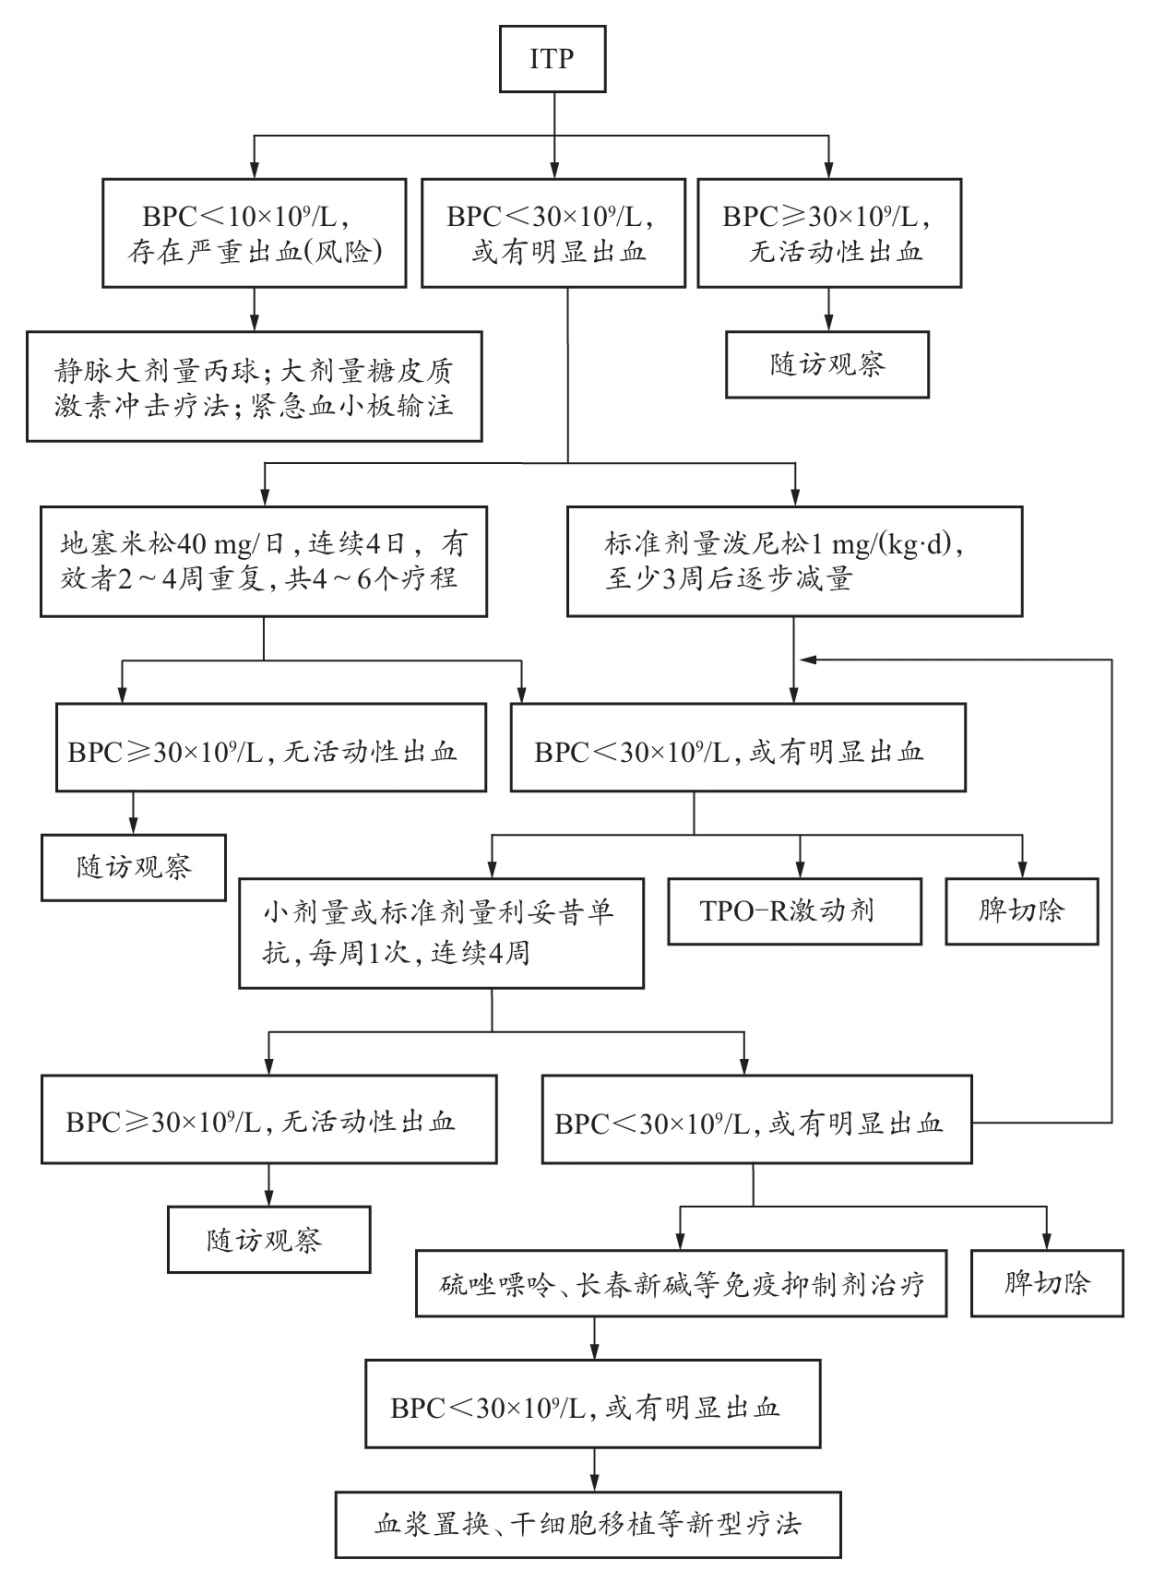
\includegraphics{./images/Image00169.jpg}
 \captionsetup{justification=centering}
 \caption{原发免疫性血小板减少症的治疗程序}
 \label{fig5-5-1}
  \end{figure} 

【治疗方案】

1.
一般治疗 对急性出血严重者,应注意休息,防止各种创伤性出血,尤其是颅内出血。可用一般止血药,如酚磺乙胺(止血敏)、卡巴克络(安络血)等。出血严重时可输血小板悬液,慢性反复出血者,如女性患者月经过多,可予铁剂治疗。忌用阿司匹林、双嘧达莫(潘生丁)等影响血小板功能的药物。

2. 药物治疗

(1)糖皮质激素:为治疗ITP的主要首选药物。如泼尼松1~2mg/(kg·d),顿服或分次口服,至少3周,待血小板数\textgreater{}30×10$^{9}$
/L时,每周减少日服量5mg,减至剂量15~20mg/d,每周减少日服量5mg,减至剂量5~10mg/d维持,共3~6个月,或每周减少日服量2.5mg,或每2周减少日服量5mg,直至减完。

(2)免疫抑制剂:采用脾切除无效或复发的患者可再次考虑应用糖皮质激素;仍无效或不能耐受者可应用免疫抑制剂治疗,常用药物有硫唑嘌呤、长春新碱、环磷酰胺和霉酚酸酯(骁悉)。如硫唑嘌呤常用剂量为每日50~150mg,一般需治疗数月后才见疗效,该药较为安全,可长时间应用维持量,但完全缓解者不多见,并需检测血象和肝功能;环磷酰胺(CTX):口服量每日50~200mg;或静脉注射,每隔3~4周1次,每次400~600mg。一般需3~6周才获效果,血小板回升后再维持4~6周。

(3)达那唑:为雄激素衍生物,对其他治疗疗效不佳的患者,部分病例可获得满意的效果。剂量为0.1~0.2g,每日2~4次。有效者一般在用药2~6周后血小板数开始升高,6~10周达高峰。达那唑需逐步减量,以维持安全止血水平的血小板数为宜。达那唑与泼尼松有协同作用,合用时可减少泼尼松用量,尤其适用于需较大量泼尼松维持治疗的患者。但应注意其对肝脏的毒性。定期监测肝功能。

(4)抗CD20单克隆抗体(利妥昔单抗):对于激素无效或无法耐受的患者同时又不愿意采用脾切等创伤性治疗的患者可以考虑使用该新型药物。抗CD20单抗(美罗华)100mg(小剂量)或375mg/m$^2$
(标准剂量),静脉滴注,每周1次,连续4周。

(5)血小板生成素受体激动剂:对于激素无效或无法耐受的患者同时又不愿意采用脾切等创伤性治疗的患者可以考虑使用该新型药物。AMG531
1~10μg/kg,皮下注射,每周1次;Eltrombopag
50~75mg/d,口服。

3.
脾切除术 是治疗本病较有效的方法之一。完全缓解率60\%~80\%。对糖皮质激素无效或依赖者、出血症状顽固或危及生命者宜尽早进行脾切除。约10\%的脾切除无效或复发的患者是由于副脾的存在,所以在手术中若发现副脾应一并切除。

4.
急症处理 患者有严重的粘膜出血(如口腔血疱)或脑出血,或疑有脑出血、BPC<10×10$^{9}$
/L时应该住院,并立即开始治疗,降低致命性出血发生率和死亡率。可采用输注单采血小板,每次10~20U或0.2U/kg;大剂量IVIG2g/kg(总量),分5日或2日给予,1个月后可重复;大剂量甲泼尼龙(HD-MP)1.0g/d,3~5日或1.0~2.0g/d,2~3日;血浆置换:每次置换3000ml血浆,在3~5日内连续3次以上。

5.
ITP孕妇的治疗 孕妇中ITP的发生率高于正常人群,由于地塞米松、长春碱类、利妥昔单抗、血小板生成素受体激动剂都可能对胎儿产生影响,因此应尽量避免使用,对于ITP孕妇的初始治疗可采用低剂量的泼尼松10~20mg/d进行治疗以维持相对安全的血小板计数,对于泼尼松疗效不佳的患者可以采用静脉用丙种球蛋白进行治疗,待血小板恢复后可以定期使用丙球进行维持治疗。

【疗效观察与随访】

1. 观察指标 血常规、血小板、骨髓常规、出凝血指标、紫癜分布等。

2.
治愈标准 血小板恢复正常、无出血症状、紫癜消失、持续3个月以上,如维持2个月以上无复发为基本治愈。

3.
随访 观察皮肤粘膜有无明显出血点、头昏乏力程度等症状。定期监测血常规变化,决定下一步治疗方案,综合评估疗效。

【治疗经验与解析】

1.
由于临床上存在少数由于EDTA抗凝导致的假性血小板减少症患者,因此对于血常规检查出现明显血小板异常,而临床症状不符合的患者,推荐使用肝素抗凝采血管复查血常规。

2. 欧洲慢性ITP诊治指南中推荐血小板数的安全值在口腔科检查≥10×10$^{9}$
/L,拔牙或补牙≥30×10$^{9}$ /L,小手术≥50×10$^{9}$ /L,正常经阴分娩≥50×10$^{9}$
/L,剖宫产≥80×10$^{9}$ /L,大手术≥80×10$^{9}$ /L。

3.
难治性ITP患者需要寻找可能存在的潜在病原体,包括血清学或呼吸试验以确定胃部幽门螺杆菌感染,血清学或分子生物学确定HCV或HIV感染等,并采取相应的治疗。

\paragraph{血栓性血小板减少性紫癜}

血栓性血小板减少性紫癜(TTP)是一种以全身性微血管血小板异常聚集、减少及红细胞机械性受损为主要特征的血栓性微血管病。目前认为TTP的发病与血管性血友病因子裂解酶(vWF-CP)即ADAMTS-13活性的绝对或相对缺乏以及针对ADAMTS-13自身抗体的产生,异常超大分子量的vWF多聚体(UL-vWF)不能被正常降解,后者可以促进血小板粘附与聚集并形成微血栓。本病主要临床表现为微血管病性溶血性贫血、血小板减少性出血、神经精神症状、肾脏损害和发热五联征。溶血性尿毒综合征(HUS)在成人和小儿均可发病,但多见于儿童与婴儿,尿毒症表现更为突出,少有发热与严重神经精神症状,其病理基础几与TTP无异,近来认为两者并入TTP/HUS综合征。

【治疗程序】 如图\ref{fig5-5-2}所示。

\begin{figure}[!htbp]
 \centering
 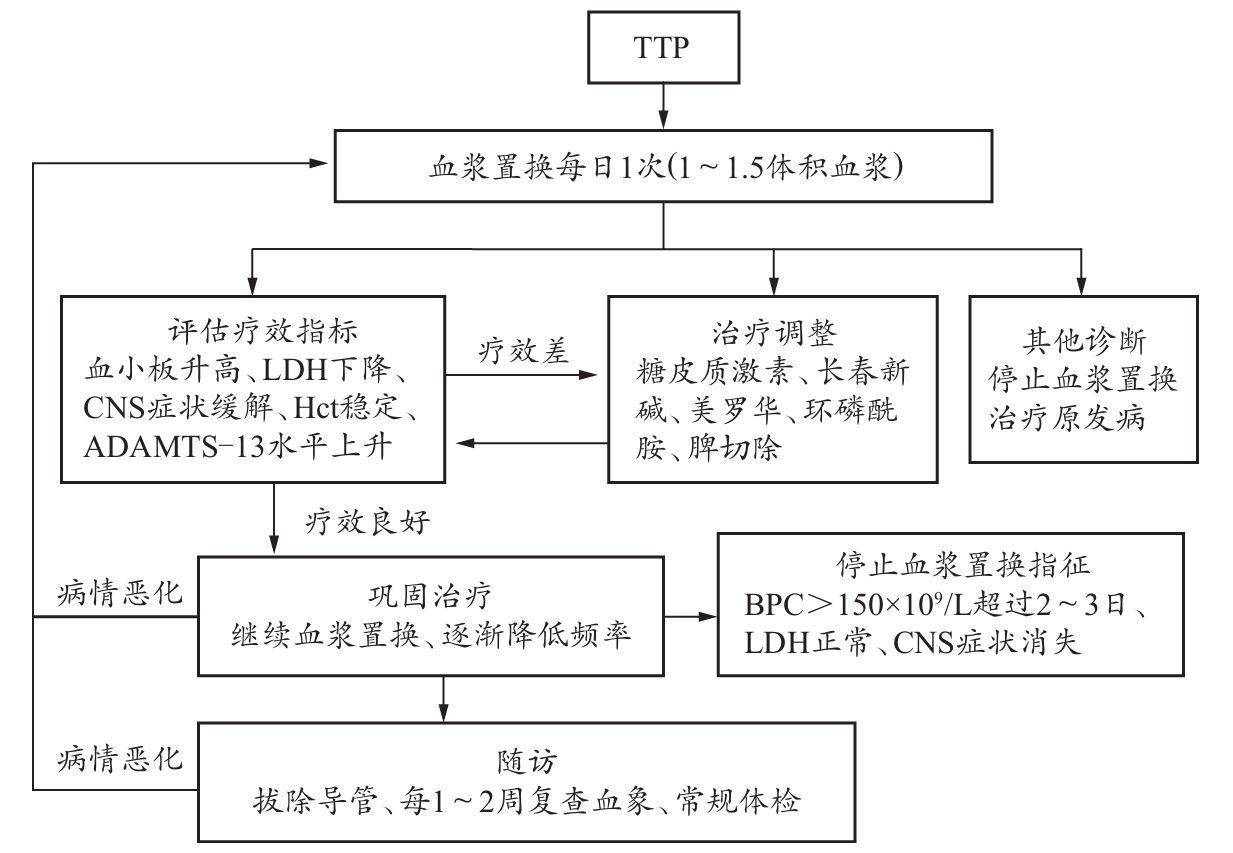
\includegraphics{./images/Image00170.jpg}
 \captionsetup{justification=centering}
 \caption{血栓性血小板减少性紫癜的治疗程序}
 \label{fig5-5-2}
  \end{figure} 

【治疗方案】

1.
血浆置换 可以有效清除UL-vWF和可能存在的ADAMTS-13自身抗体,并补充ADAMTS-13,为TTP抢救和治疗首选方案,置换液一般采用新鲜冰冻血浆(FFP)。

治疗原则:①早期:由于TTP发病凶险,死亡率高因此应尽早开始,一旦高度怀疑本病时即应开始给予血浆置换;②足量:血浆置换量应以单个血浆容积(40ml/kg)作为基础日交换量。推荐进行每日血浆置换,开始治疗的前2日,每日置换1.5个血浆容积(60ml/kg),以后每日置换1个血浆容积(40ml/kg),直至疗程结束。③联合:对于自身免疫因素导致机体产生ADAMTS-13抑制物的TTP可以在进行血浆置换的同时联合糖皮质激素、IVIG、免疫抑制剂和利妥昔单抗(美罗华)等进行联合治疗。

2.
糖皮质激素 有助于稳定血小板和内皮细胞膜,抑制ADAMTS-13自身抗体的产生。除非患者有糖皮质激素使用禁忌证,一旦诊断确立,建议在应用血浆置换的同时使用糖皮质激素,直至病情缓解。如泼尼松1mg/kg,口服,每12小时1次或甲泼尼龙1000mg,静脉滴注,每日1次,用3日后减量或改为口服泼尼松维持。

3.
利妥昔单抗 对于多次血浆置换效果欠佳,或者初治疗效尚可,但是疾病反复复发的TTP患者可以考虑使用利妥昔单抗进行治疗;此外对于初治TTP患者有明确自身免疫因素导致的ADAMTS-13活性下降可以考虑在血浆置换同时联用糖皮质激素和利妥昔单抗,使用方法建议在血浆置换后使用利妥昔单抗以保证体内有效药物浓度。如抗CD20单抗(美罗华)375mg/m$^2$
,静脉滴注,每周1次,连用4周。

4.
长春新碱(VCR) 目前主要用于难治复发性TTP的治疗。如长春新碱1.4mg/m$^2$
(最大2mg),静脉注射,d1,d8。

5.
脾脏切除 对于部分反复发作的TTP,切除脾脏可以去除了扣押破坏血小板和红细胞的场所,也去除了致病抗体的产生部位,在部分难治的患者中有效。

6.
血液透析 发生急性肾衰竭的患者提倡尽早进行透析治疗。HUS患者无尿持续时间越长,肾功能恢复机会越少。

【疗效观察与随访】

1.
观察指标 观察皮肤粘膜的出血情况,神经精神异常的变化。根据血小板、LDH、Hct、ADAMTS-13水平的变化,综合评估疗效。

2.
治愈标准 症状与体征消失,出血停止,相关检测指标恢复正常,3个月内未复发。

3.
随访 注意观察病情,观察症状体征的变化,避免再次接触致病因素,避免并发症,定期复查相关指标。

【治疗经验与解析】

1.
TTP分为遗传性TTP和继发性TTP,临床上常见的TTP是由于机体产生ADAMTS-13抑制物或者各种病原体严重感染、恶性肿瘤等因素所导致的继发性TTP。

2.
由于TTP发病凶险,病情进展迅速,因此临床只要高度怀疑TTP,出现微血管病性溶血和血小板减少表现,并排除DIC、ITP、Evans综合征、子痫等类似病症后,即可开始血浆置换治疗。

3.
对于TTP患者发生的贫血和血小板减少一般不提倡积极输注红细胞和血小板,除非出现致命性出血或颅内出血。

4.
儿童腹泻后出现的微血管病性溶血和血小板减少,多诊断为腹泻相关性HUS,通常无特殊治疗,抗生素、止泻药可能会加重病情,应避免应用。

\subsection{凝血因子疾病}

\paragraph{血友病}

血友病是由于先天性血浆凝血因子缺乏或功能缺陷致血浆凝血活酶生成障碍而引起的一组伴性遗传性出血性疾病,绝大多数血友病为男性患者。血友病分为由于凝血因子Ⅷ(FⅧ)缺乏造成的血友病A和凝血因子Ⅸ(FⅨ)缺乏造成的血友病B。该病自幼起病,临床表现关节和内脏出血,我国血友病中以血友病A为常见,约占到血友病总数的80\%。

【治疗方案】 以预防为主,患者应该定期监测APTT和FⅧ:C含量,及时补充缺乏的凝血因子,防止严重致命性出血的发生。

1.
预防出血 加强宣教,避免创伤及较重的体力活动。美国国家血友病基金会对重型血友病患儿进行早期预防性治疗,维持FⅧ:C或FⅨ:C\textgreater{}1\%。推荐剂量:FⅧ(25~40)U/kg,每周3次;FⅨ(25~40)U/kg,每周2次。

2.
替代疗法 新鲜血浆或新鲜冰冻血浆(FFP);冷沉淀物(CPT);FⅧ浓缩剂或FⅨ浓缩剂;基因重组FⅧ或FⅨ。

新鲜血浆或新鲜冰冻血浆(FFP)1ml正常新鲜血浆中FⅧ或FⅨ的含量相当于1UFⅧ或FⅨ。成人一次最大用量为20ml/kg,因容量因素使血浆在血友病的应用受到限制,目前作为替代治疗已少用。

冷沉淀(CPT)适用于轻中型血友病A患者,每袋20ml冷沉淀制剂取自200ml新鲜血浆,具有容量小而效力大的特点。不足之处在于冷沉淀中含有少量红细胞及碎片,易引起抗原抗体反应,部分患者输注后产生血型抗体,且病毒未被灭活。

凝血酶原复合物浓缩剂(PCC)多用于血友病B。每瓶200U规格,相当于200ml血浆中所含有的FⅨ。

FⅧ浓缩剂或FⅨ浓缩剂:FⅧ浓缩剂根据来源分为人型和猪型两种,猪型FⅧ浓缩剂多用于产生了FⅧ抗体的患者。每输入1U/kg的FⅧ,可使患者FⅧ:C活性水平提高2\%,推荐输入FⅧ浓缩剂剂量(U)=0.5×体重(kg)×预期增加值(\%)。但由于FⅨ浓缩剂回收率低,每输入1U/kg的FⅨ,可使患者FⅨ:C活性水平提高0.5\%~1\%,推荐输入FⅨ浓缩剂剂量(U)=1.2×体重(kg)×预期增加值(\%)。FⅧ:C半衰期8~12小时,补充FⅧ需连续(持续)或每8~12小时1次,静脉滴注。FⅨ半衰期18~30小时,补充FⅨ只需每日1次静脉滴注即可。血友病各种出血替代治疗用量及相应其他治疗见表\ref{tab5-5-1}。

\begin{longtable}[]{p{3cm}p{5cm}p{5cm}}
    \caption{血友病各种出血替代治疗用量及相应其他治疗}
    \label{tab5-5-1}\\
\toprule
出血表现 & 血友病A:输注FⅧ & 血友病B:输注FⅨ\tabularnewline
\midrule
\endfirsthead
\caption[]{血友病各种出血替代治疗用量及相应其他治疗}\\
\toprule
出血表现 & 血友病A:输注FⅧ & 血友病B:输注FⅨ\tabularnewline
\midrule
\endhead
\bottomrule
\endfoot
关节出血 &首次20~50U/kg;若尽早治疗,可用15U/kg;若出血严重,第2日重复输注,然后可隔日1次,持续1周;对于轻、中型血友病,若已知患者对DDAVP有反应,应使用DDAVP(0.3μg/kg)代替FⅧ&首次30U/kg;若尽早治疗,可用20U/kg;若出血严重,第2日重复输注;然后可隔日1次,持续1周\tabularnewline
肌肉血肿或严重的皮下血肿 & 首次20U/kg,然后隔日1次,直至血肿完全吸收 &
首次30U/kg;然后每2~3日1次,直至血肿完全吸收\tabularnewline
口腔粘膜出血或拔牙 & 首次20U/kg,并加抗纤溶药物 &
首次30U/kg,并加抗纤溶药物。抗纤溶药物应在输注凝血酶原复合物4~6小时后使用\tabularnewline
鼻出血 &
压迫止血15~20分钟;凡士林纱布填塞;抗纤溶药物;必要时20U/kg输注
&
压迫止血15~20分钟;凡士林纱布填塞;抗纤溶药物;必要时30U/kg输注\tabularnewline
大手术,危及生命的出血(CNS出血、消化道出血,呼吸道出血等) &首次50~75U/kg,然后3U/(kg·h)维持;第1日因子水平维持在100\%以上;第2日2~3U/(kg·h)维持,连续用药5~7日,因子水平维持在50\%以上;继续用药5~7日,因子水平维持在30\%左右&首次80U/kg,然后20~40U/kg,每12~24小时1次,因子水平维持\textgreater{}40\%,持续5~7日继续用药5~7日,因子水平维持在30\%左右\tabularnewline
腹膜后或髂腰肌出血&首次50U/kg,然后25U/kg,每12小时1次,直至症状消失;以后20U/kg,隔日1次,总天数10~14日。在停止治疗前应反复进行放射学评价&首次80U/kg,然后20~40U/kg,每12~24小时1次,直至症状消失;以后30U/kg,隔日1次,总天数10~14日。在停止治疗前应反复进行放射学评价\tabularnewline
\end{longtable}

3.
醋酸去氨加压素(DDAVP) 因为DDAVP可以刺激内皮细胞释放vWF和FⅧ,因此可以用于轻中型血友病A或血管性血友病患者的出血。用法为:DDAVP0.3~0.4μg/kg,加入20~40mlNS或5\%GS,静脉滴注持续20~30分钟,每12小时1次。

4.
抗纤溶药物(纤溶抑制剂) 对皮肤粘膜出血尤其口腔出血的效果较好,对内脏、关节、肌肉的出血无效。此外由于抗纤溶药物多经过泌尿系统以原形形式排出,因此对于泌尿道出血,不主张使用抗纤溶治疗以防止堵塞尿道。用法:氨基己酸(EACA)50~100mg/kg,静脉滴注,每日1次;或止血环酸20~40mg/kg,静脉滴注,每日1次。

5.
肾上腺糖皮质激素 尤其适用于反复接受FⅧ输注产生FⅧ抑制物而疗效渐差的患者,尚有控制血尿、促进急性关节出血吸收,减少局部炎症反应辅助作用。

6.
达那唑 为人工合成雄性激素,可提高因子Ⅷ水平。年龄<15岁时,300mg/d,连续14日,口服;年龄\textgreater{}15岁时,600mg/d,连续14日,每日分3次口服。

7.
血友病合并抑制物的处理 在获得性凝血因子抑制物中最常见的是FⅧ抑制物。对于遗传性血友病A患者,由于要长期补充FⅧ,因此治疗过程中产生FⅧ抑制物的发生率为10\%~20\%。血友病B患者FⅨ抑制物的发生率约为3\%,重型患者可高达12\%。当临床应用足量因子Ⅷ治疗后,出血仍持续甚至加剧,应考虑抗Ⅷ因子抗体的产生。

(1)大剂量的FⅧ替代治疗:人型或猪型FⅧ浓缩剂均有效,大剂量浓缩物足以中和抑制物,且提供多余的FⅧ,使血浆FⅧ≥0.3U/ml。但对于产生了FⅧ抗体的患者多用猪型FⅧ浓缩剂。推荐剂量hFⅧ20U/(kg·Bu)抑制物,再加40U/kg,静脉滴注(高反应\textgreater{}5Bu和低反应<5Bu),可同时加用肾上腺皮质激素、IVIG或免疫抑制剂如CTX等。

(2)旁路治疗:

1)重组活化FⅦ(rFⅦa,诺其):大量的FⅦ可以激活机体内源性凝血途径,产生凝血酶从而达到止血的效果。rFⅦa也可用于防治产生了FⅧ或FⅨ抗体的血友病患者的出血,推荐rFⅦa90~100μg/kg,静脉滴注,每2~4小时1次,直至出血停止,85\%~100\%有效,但有促进血栓形成的副作用。

2)凝血酶原复合物浓缩剂(PCC):PCC50~100U/kg或活化的凝血酶原复合物浓缩剂(APCC)50~70U/kg,每12~24小时1次,止血效果达60\%~95\%。

(3)近年来有报道对于难治性FⅧ抑制物可以考虑使用利妥昔单抗进行治疗,但是由于方法较新,缺乏大样本临床研究数据,具体用法和疗程尚未统一。

8.
血友病A基因携带者妊娠后的处理 血友病A基因携带者的FⅧ:C水平往往仅为正常人的50\%左右,产程中部分血友病A基因携带者会出血,也可表现为产后出血,产前进行严密准备,胎儿娩出后产妇若有出血倾向,应即予以输注FⅧ制剂。

9. 外科治疗 关节固定及理疗、关节成形及人工关节置换术。

【疗效观察与随访】

1.
观察指标 常见症状与体征,出血部位、范围,血小板及出凝血指标、凝血因子等。

2.
疗效评估 本病虽然为终身性疾病,但随着近年来各种治疗方法的出现及进展,预后得到了显著改善,生活质量得到提高。

3.
随访 观察疗效主要是两方面:①出血症状的改善及消退情况;②FⅧ:C水平达到止血要求,一般达正常人的60\%~120\%。

【治疗经验与解析】

1.
对于血友病患者应该加强宣教,以预防为主,定期监测各项相关指标,推荐预防性输注,防止致命性出血的发生。

2.
血友病患者尽量避免手术,如必须施行,术前做好充分准备。凝血严重异常者尽量避免肌内注射或皮下注射,静脉穿刺至少压迫10~15分钟。慎用阿司匹林、双嘧达莫、吲哚美辛等抑制血小板功能的药物。

\paragraph{血管性血友病}

血管性血友病(vWD)是由于von
Willebrand因子(vWF)质或量的异常而导致的出血性疾病,是常见的遗传性出血性疾病之一,多数患者为显性遗传,少数患者为隐性遗传,两性均可发病。出血以皮肤、粘膜、齿龈、内脏出血为主,很少累及关节腔及深部肌肉。

【治疗方案】 根据最新分型标准,vWD分为三型:1型、2型(2A、2B、2M、2N)及3型。1型和3型是vWF量的减少,其中1型为部分减少,3型为重型减少,2型是vWF质的异常。治疗程序参见血友病节。

vWD的治疗原则是对于轻型患者主要以避免外伤、手术和抗血小板药物造成的出血,对于有明显出血的患者可以使用替代疗法和相应的对症处理。

1.
1-去氨基-8D-精氨酸加压素(DDAVP) 为人工合成的加压素衍生物。可促使血管内皮细胞释放FⅧ:C,促进VEC释放vWF:Ag,增加FⅧ:C稳定性,并改善血小板粘附功能。对大多数1型和2型患者有效,2B型vWD患者由于vWF和血小板GPIb的结合能力上升,因此不宜使用DDAVP治疗以防止血栓形成。

2. 替代疗法

(1)冷沉淀物(CPT):为替代治疗首选制剂。CPT中含FⅧ/vWF及纤维蛋白原,且vWF含量较FFP高5~10倍,能缩短出血时间及提高FⅧ:C。vWD患者大手术前给予FⅧ50U/kg(使血浆中FⅧ水平达到100\%),随后可每12小时输注半量。中度vWD患者术后24小时给冷沉淀,可达较好的止血目的。

(2)新鲜冰冻血浆(FFP):FFP10~15ml/kg可使血中FⅧ:C或活性达75\%以上,同时能纠正出血时间延长。vWF半衰期为24小时,必要时每24~48小时输血浆1次,每次5ml/kg。术前输400~600ml血浆,可使出血时间维持在2~4分钟内。

(3)Ⅷ因子浓缩物:能提高Ⅷ:C,但高纯度Ⅷ因子制剂中缺少与vWF活性有关的高分子多聚体,不能纠正出血时间延长。治疗效果不佳的vWD患者可改用vWF-Ⅷ因子浓缩物治疗。对于大多数急性失血、拔牙的vWD患者,输注1个剂量的浓缩剂,可提高血浆vWF:RCO50\%,便可达到治疗效果,但对患有严重vWD患者进行外科手术时,首次剂量要使血浆vWF:RCO提高到100\%,随后用半量,每12h给药1次,使vWF:RCO维持在50\%以上,对于中度vWD的患者剂量可稍减。

3.
辅助治疗 局部出血可以采用加压止血,鼻出血及时填塞,以及可以采用明胶海绵、凝血酶等止血。对于女性患者出现月经过多,可口服雌孕激素。

【疗效观察与随访】 参见血友病节。本病患者出血主要是由于vWF:Ag量与质的异常和FⅧ:C活性的减低,因此在患者接受冷沉淀输注和DDAVP治疗时需监测出血时间、APTT、vWF:Ag和FⅧ:C以评估疗效,判断是否达到止血的需求。

【治疗经验与解析】

1. 本病禁用水杨酸类药物等影响血小板功能的药物。

2.
本病病程长,但出血可以随着年龄增加而减轻。虽然出血常表现为皮肤粘膜出血,但需要注意脑出血以及其他危及生命的内脏出血。

\paragraph{肝脏疾病凝血障碍}

肝脏疾病凝血障碍是指由于各种原因导致肝功能严重受损所致的血液凝血系统功能异常,临床主要表现为患者具有明显的出血倾向,在少部分患者由于肝脏对于抗凝蛋白的灭活能力减弱也可能表现为局部的高凝状态或血栓形成。肝脏疾病凝血障碍产生的主要原因为肝脏是合成大多数凝血因子的器官,肝功能受损会导致各种凝血因子合成减少;其次肝硬化患者机体的纤溶活性是明显增强的,肝脏对于组织型纤溶酶原活化物(t-PA)和尿激酶型纤溶酶原活化物(u-PA)的灭活和清除能力减低;肝脏对于体内肝素样物质灭活减弱、弥散性血管内溶血等都会增加机体出血风险。

此外肝硬化患者往往伴有脾功能亢进,进而导致血细胞尤其是血小板的减少进一步加重了患者的出血可能。

【治疗程序】 肝脏疾病凝血障碍临床表现为比较明显的出血风险,实验室检查异常主要包括PT、aPTT延长(以PT延长更为明显)、纤维蛋白原下降、TT延长,FDP升高;t-PA,纤溶酶水平升高,纤溶酶原活化剂抑制物(PAI)含量下降。

对于肝脏疾病凝血障碍的治疗主要是在积极治疗原发肝脏疾病的基础上,使用包括新鲜冰冻血浆(FFP)、纤维蛋白原、冷沉淀和单采血小板等在内的血制品输注的替代疗法补充机体缺乏的凝血因子,纠正凝血异常。

【治疗方案】

1. 积极治疗原发肝脏疾病、尽快恢复或部分恢复肝功能。

2.
补充凝血因子 新鲜冰冻血浆输注因为含有多种机体凝血所必需的因子,因而常作为治疗肝脏凝血障碍治疗的一线疗法,输注量一般为5~10ml/kg,可以提高10\%~20\%机体凝血因子的活性,虽然有时不足以纠正异常的PT和aPTT,但是可以明显改善临床症状和降低出血的风险。对于纤维蛋白原明显减低的患者可输注纤维蛋白原或冷沉淀,维持纤维蛋白原在1.5g/L以上。维生素K缺乏患者积极补充维生素K。

重组人FⅦa可以用以治疗血制品输注无效的严重出血,剂量一般为25~50μg/kg,但是由于rFⅦa半衰期较短,因此虽然暂时可以纠正异常的凝血指标,但是必须序贯较为持久的措施达到长久止血的目的。

3. 单采血小板输注 通常当血小板低于20×10$^{9}$
/L时推荐输注血小板,但有学者认为肝病患者血小板可能存在功能障碍,因此对于有严重凝血因子缺乏并且出血表现的患者推荐通过输注血小板使外周血血小板大于50×10$^{9}$
/L。

4.
其他辅助治疗 可以通过鱼精蛋白中和体内过多的肝素或肝素样物质,通常1mg鱼精蛋白中和1mg肝素;FDP增高的原发性纤溶亢进患者可以予以适当抗纤溶治疗。

【疗效观察与随访】 对于肝脏疾病凝血障碍疗程观察主要是临床出血症状的改善和凝血指标的恢复。其中PT是对于肝病相关的凝血异常较为敏感的指标之一。

【治疗经验与解析】

1. 肝脏疾病凝血障碍的治疗需要首先处理肝功能损伤、脾亢、感染等因素。

2.
反复多次和大剂量的FFP输注会导致患者血容量过多,此时可以通过输注纤维蛋白原、冷沉淀和rFⅦa减少输注量。

\subsection{血栓形成和血栓栓塞性疾病}

血栓形成和血栓栓塞性疾病,简称血栓栓塞性疾病,是由于先天遗传性或后天获得性原因导致患者止血与抗血栓机制失衡,循环血液中有血栓形成及血栓从局部脱落随血流至前方血管内,造成血管腔阻塞的疾病从而引起相应组织缺血、缺氧甚至坏死的病理生理过程。临床上将血栓分为动脉血栓、静脉血栓、动静脉血栓和微血管血栓。

近年来又提出易栓症概念,易栓症是指由于抗凝因子、纤溶活性等遗传性或获得性缺陷而机体易于发生血栓形成的一类疾病。

【治疗方案】 血栓形成的治疗,首先是去除可能存在的高危因素,包括治疗和控制感染、肿瘤、动脉粥样硬化、糖尿病、恶性肿瘤和药物如肝素、避孕药、抗纤溶剂等血栓形成的高危因素,并且进行适当的抗血小板和(或)抗凝治疗,防止发生脏器功能损伤。

1.
抗凝治疗 无论诱因是否可以去除,对于已经发生的血栓栓塞尤其是包括深静脉血栓和肺静脉栓塞的患者需要尽快进行常规的抗凝治疗防止再次发生血栓事件,使用的药物包括低分子量肝素、肝素和华法林等。对于抗凝周期目前尚无定论,一般认为对于高危因素可以去除的患者推荐至少抗凝两个月,对于具有明确高危因素并且难以去除的患者推荐至少半年甚至终身抗凝。

(1)低分子量肝素用法:预防性使用50~100U/(kg·d),分2次皮下注射;治疗性使用200U/(kg·d),分2次皮下注射。

(2)华法林:是PTE和VTE长期治疗的首选治疗药物。在使用低分子肝素钠或肝素钠治疗的第1日即开始联合应用华法林。用法:起始剂量为3~5mg/d,1周后监测PT,使PT-INR维持在1.5~2.5之间。

(3)肝素钠的用法:预防性使用10000~20000U/d,分3~4次使用,静脉滴注,监测APTT,使延长1~2倍较为合适;治疗性使用30000~40000U/d,分3~4次使用,静脉滴注,监测APTT,使其延长1.5~2.5倍较为合适。

2.
抗血小板治疗 尤其对于动脉血栓形成的患者,阿司匹林的使用可以明显降低此类患者动脉血栓的再栓塞率,显著提高患者生活质量和生存。预防性使用阿司匹林予75mg/d,口服;治疗性使用予300mg/d,口服。

3.
溶栓治疗 应用于新近形成的血栓,尤其是包括心梗在内的动脉血栓,一般而言对于动脉血栓最好于血栓事件发生后3小时内进行溶栓,最晚不要超过6小时,而静脉血栓应尽量在发病72小时内进行溶栓,最晚不要超过1周。使用禁忌证包括:手术和创伤后10日内,妊娠以及分娩后10日内,严重高血压和脑出血2个月内,活动性溃疡和肺结核。

用法:尿激酶首剂4000U/kg,静脉注射后,以4000U/h维持治疗,1~3日为1个疗程。组织型纤溶酶原激活剂(rt-PA)首剂100mg,静脉注射后以每小时50mg维持,共2小时。

对于反复发生的下肢静脉血栓,并且高危因素无法去除的患者为了防止致命性肺静脉栓塞的发生,可以考虑进行下肢静脉滤网。

4.
外科(介入)治疗 对于内科治疗疗效不佳的患者可以使用外科(介入)等治疗手段使缺血缺氧的器官重新获得再灌注从而(部分)恢复脏器功能。

【疗效观察与随访】 本病的疗效因原发病而异,病因能去除者,预后相对较好,参见相关原发病。

【治疗经验与解析】

1.
对于血栓性疾病的治疗首先需要去除可能存在的导致血栓形成的危险因素,减少血栓复发的可能。

2.
由于动脉血栓溶栓窗口期较短,因此在疾病确诊后应尽快进行溶栓,防止出现重要脏器的不可逆损伤。

\subsection{弥散性血管内凝血}

弥散性血管内凝血(DIC)是在机体发生严重原发病的基础上发生微循环广泛性纤维蛋白沉积和血小板聚集,并伴有继发性纤维蛋白溶解亢进的一种获得性全身性血栓出血综合征,DIC本身只是机体严重疾病导致的一种病理生理过程,并不是一个独立的疾病。临床表现为出血、栓塞、微循环障碍及血管内溶血等。诱发DIC的基础疾病很多,其中感染性疾病、恶性肿瘤、病理产科、手术和创伤是DIC五大常见病因。

【治疗程序】 如图\ref{fig5-5-3}所示。

\begin{figure}[!htbp]
 \centering
 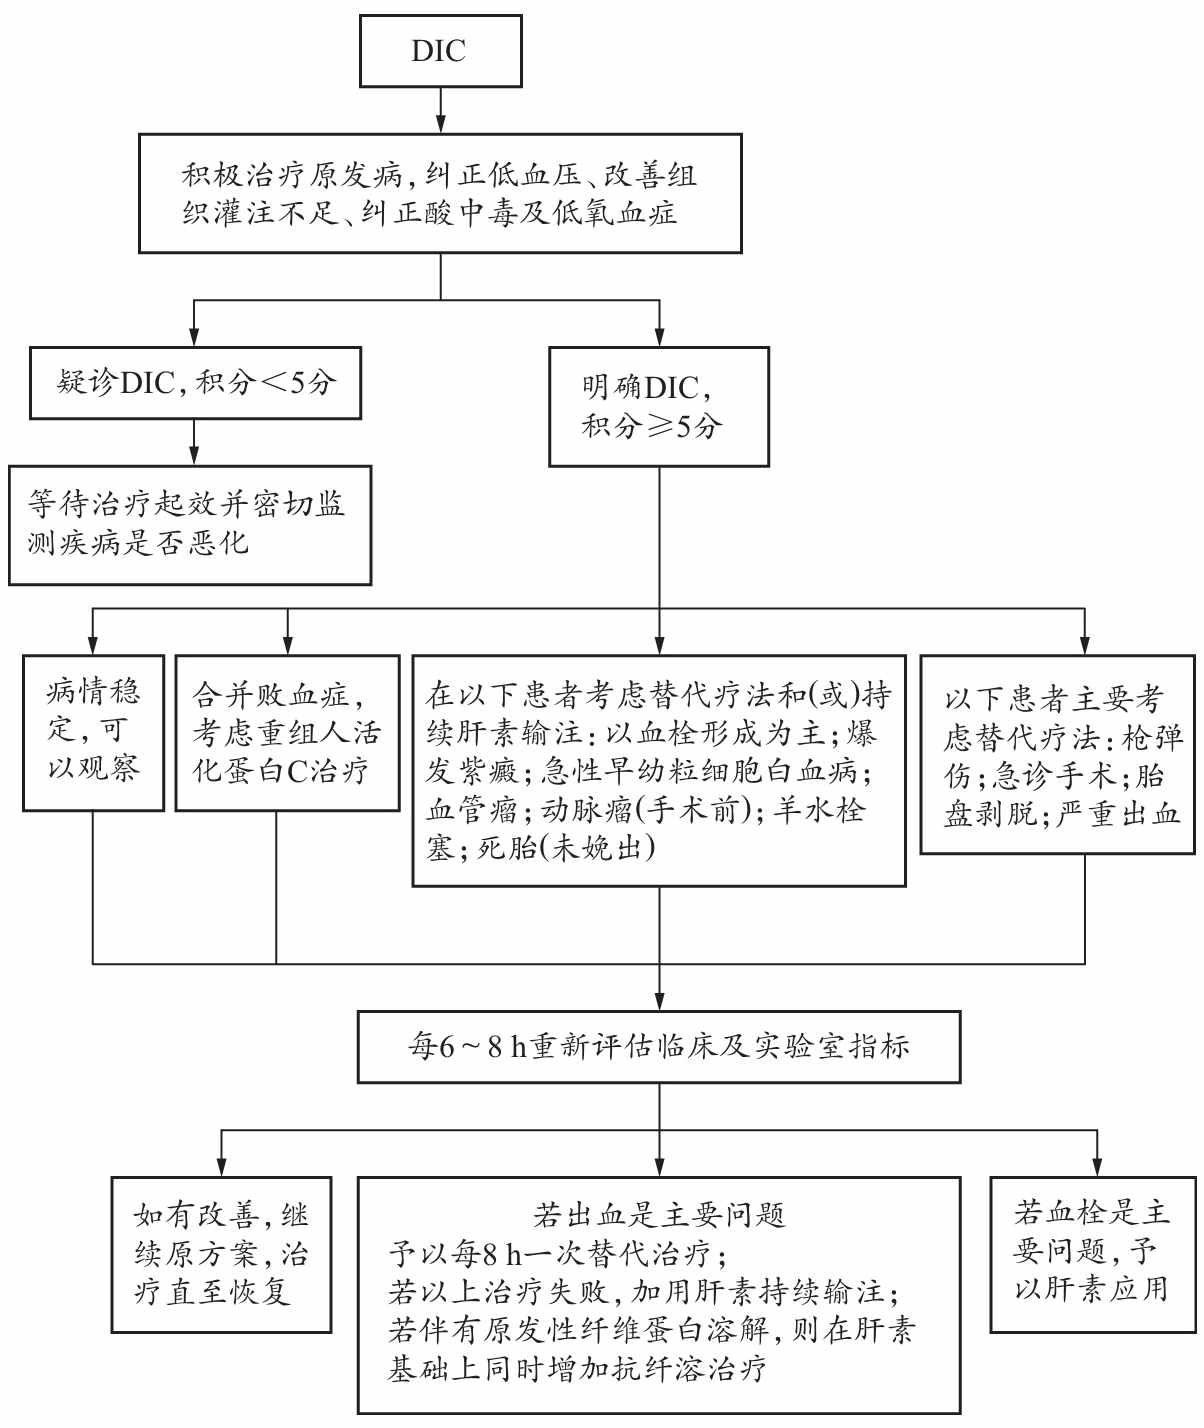
\includegraphics{./images/Image00171.jpg}
 \captionsetup{justification=centering}
 \caption{弥散性血管内凝血的治疗程序}
 \label{fig5-5-3}
  \end{figure} 

【治疗方案】

1. 一般治疗 及时有效的去除病因和诱因,治疗原发病是处理DIC的关键。

2. 药物治疗

(1)抗凝治疗:普通肝素和低分子量肝素(LMWH)。普通肝素用法:急性DIC时,首剂50~100U/kg,皮下注射,然后25~50U/kg,皮下注射,每6~8小时1次,根据凝血检查结果调整剂量;也可以应用5~15U/(kg·h),持续静脉滴注3~5日,每6小时用量不超过5000~7500U。慢性DIC和部分亚急性DIC时,予肝素钠200U/(kg·d),分3~4次皮下注射,每疗程8日。用于预防DIC时,可予肝素钠50U/(kg·d),分3~4次皮下注射,连续5~8日。

1)应用普通肝素的实验室监测指标:活化部分凝血活酶时间(APTT)使其延长并维持在正常值(40±5秒)的1.5~2倍,平均60~80秒。

2)低分子量肝素(LMWH)由于低分子量肝素对于FⅩ的抑制作用大于对凝血酶的抑制(约为4∶1),因此临床上出血的副作用较普通肝素显著降低,成为临床抗凝的主要制剂之一。LMWH抗Ⅹa活性与其抗凝能力密切相关,而抗凝血酶活性与治疗相关性出血并发症有关。虽然常规抗凝使用LMWH时无需监测APTT,但是由于DIC患者往往合并严重的凝血异常和血小板减少,因此对于DIC患者使用LMWH时,仍然推荐监测血浆APTT,标准同普通肝素。低分子量肝素:用于预防DIC时,50~100U/(kg·d),分2次皮下注射,连续5~10日;用于治疗DIC时,予200U/(kg·d),分2次皮下注射,连续5~8日。

3)新型抗凝药物:目前有多种新型抗凝制剂进入临床,包括AT-Ⅲ、重组人活化蛋白C(APC),重组可溶性TM、TFPI以及组织因子制剂等,但是由于缺乏大规模的三期临床试验验证疗效,因此临床尚未广泛使用。

(2)替代治疗:DIC中后期发生明显纤溶亢进时,机体由于大量血小板和凝血因子被消耗而产生严重的出血现象,因此替代治疗是中后期DIC治疗的重要措施之一。临床应用指征包括有明显的活动性出血、需手术治疗、FIB<1.0g/L、血小板数<50×10$^{9}$
/L的患者。

常用的替代治疗包括:

1)血小板悬液:当血小板数<30×10$^{9}$
/L时,为预防颅脑、肺部等重要器官出血,可预防性输注0.2U/kg;如伴明显出血,应使血小板数\textgreater{}50×10$^{9}$
/L。

2)FFP:含有生理需要的各种凝血因子及抗纤溶酶、AT-Ⅲ。所含的血小板及凝血因子浓度比新鲜全血高1倍。1ml/kg的FFP可使血液中凝血因子浓度升高1\%~2\%。

3)冷沉淀物:含有较多的纤维蛋白原、因子Ⅷ、vWF,尤其纤维蛋白原含量为新鲜血浆的5~10倍,适用于纤维蛋白原有明显降低的患者。但目前对于DIC患者是否需要预防性输注冷沉淀物仍然存在争论。

4)纤维蛋白原制剂:每1g纤维蛋白原可升高血浆纤维蛋白原浓度0.25g/L,因其半衰期长,96~144小时,血浆FIB恢复1.0g/L以上且无明显纤溶亢进者,一般无需重复使用。

(3)抗血小板:一般仅用于早期血液高凝状态(血栓前状态)、轻型DIC病因可迅速去除者或高度怀疑DIC而尚未肯定诊断的患者,作为DIC的辅助性治疗。

(4)纤溶抑制剂:仅适用于DIC病因已经去除或基本控制,并有明显纤溶亢进的临床及实验室证据,已行充分有效的抗凝和替代治疗,出血仍难以控制;DIC后期,血管内凝血已停止,纤溶亢进已成为再发性或延迟性出血的主要病理生理过程时,可谨慎使用抗纤溶药物。DIC早、中期或进行性DIC者禁用,有尿路出血的患者禁用纤溶抑制剂。常用的纤溶抑制剂有:止血芳酸(PAMBA)、止血环酸、6-氨基己酸(EABA)、抑肽酶等。如止血芳酸(PAMBA)0.4~0.8g/d,静脉滴注或止血环酸0.5~1.5g/d,静脉滴注。

(5)溶栓治疗:DIC患者一般无需溶栓治疗,但当机体出现明显微血栓所致的顽固性休克和重要脏器功能衰竭时,使用包括肝素在内的各种治疗无效时,可谨慎试用纤溶激活剂。常用的溶栓药物有链激酶、尿激酶及组织纤溶酶原激活剂(t-PA),其中t-PA对纤维蛋白具有高度的亲和性,其对纤溶酶原的激活在纤维蛋白表面进行,而对循环中的纤溶酶原及凝血因子无影响,故安全性较好,无明显副作用。

(6)糖皮质激素:适用于基础疾病需要用其治疗者,如溶血反应、变态反应性疾病;感染中毒性休克合并DIC,在积极抗感染基础上或已行抗感染有效者;伴有肾上腺皮质功能不全者。可应用氢化可的松100~300mg/d或地塞米松5~10mg/d,分1~2次静脉滴注。

【疗效观察与随访】

1.
观察指标 出血情况、血压变化、休克、脏器功能不全、血小板计数、纤维蛋白原含量及其他凝血象和FDP等检测。

2.
治愈标准 出血、休克、脏器功能不全等DIC表现消失,低血压、瘀斑等体征消失,相关检测指标恢复正常,病情稳定1周以上。

3.
随访 对DIC患者,重要生命指征应当每4小时检查1次,DIC实验室指标应每8小时复查1次,从而动态判断患者对治疗反应,及时调整治疗措施。DIC预后判断取决于原发疾病严重程度,DIC失代偿情况以及机体重要脏器的功能和代偿障碍程度。注意病情观察,避免致病因素。

【治疗经验与解析】

1.
DIC治疗最为重要的就是积极治疗和去除原发疾病,只有在原发疾病得到较好控制的前提下,DIC才会逐渐好转。

2.
替代治疗必须在病因治疗和充分抗凝治疗的基础上进行。尤其在DIC早期,如未行抗凝治疗而单纯补充血小板和凝血因子,往往有可能加重病情。
